\chapter{Kombinationen aus \textit{halt} und \textit{eben}}
\label{chapter:hue}
\section{Die Einzelpartikeln \textit{halt} und \textit{eben} in der Literatur}
\label{sec:hueinliteratur}
M.E. lassen sich in der Literatur zu den Einzelpartikeln \textit{halt} und \textit{eben} zwei generel\-le Ansichten unterscheiden: Die eine vertritt die Idee, dass die Bedeutung der beiden MPn identisch ist und der Unterschied zwischen ihnen in ihrer regional verschiedenen Verwendung liegt. Die andere geht davon aus, dass die Bedeutung zwar ähnlich ist, es aber auch Unterschiede gibt. Ich schließe mich der letzteren Ansicht an, wenngleich man anerkennen muss, dass es früher regionale Unterschiede gegeben hat. Da der Aspekt der regionalen Unterschiede dem Thema anhaftet und es (wie wir in Abschnitt~\ref{sec:anlit} sehen werden) auch Aussagen über die Kombination von \textit{halt} und \textit{eben} vor diesem Hintergrund gibt, möchte ich im folgenden Abschnitt einige Annahmen zu dem Thema regionaler Varianten skizzieren.

\subsection{Regionale Varianten}
\label{sec:regio}
Es gibt ältere Untersuchungen, die zu zeigen behaupten, dass es regionale Unterschiede zwischen dem \textit{halt}- und \textit{eben}-Gebrauch im deutschsprachigen Raum gegeben hat. Die meines Wissens erste Beobachtung dieser Art geht zurück auf \citet{Eichhoff1978} im \textit{Wortatlas der deutschen Umgangssprache}. Es handelt sich hierbei um eine Erhebung (vor allem im Lexembereich), die die Absicht verfolgte, regionale Verwendungsunterschiede in Deutschland, Österreich und der Schweiz zu erfassen. In Form der Frage in (\ref{538}) waren auch \textit{halt} und \textit{eben} Teil dieser Untersuchung.

\begin{exe}
	\ex\label{538} Frage 113\\
    Setzt man \textit{halt} oder \textit{eben} oder einen anderen Ausdruck in einem Satz wie: \glqq Der Zug fährt erst in einer Stunde, da muß ich .......... so lange warten?\grqq{} Wenn ja, bitte setzen Sie ein.
\hfill\hbox{\citet[31]{Eichhoff1978}}    
\end{exe}
Die Ergebnisse werden in \citet{Eichhoff1978} jeweils durch Karten der Art in Abbildung \ref{Abbildung 1} präsentiert.

\begin{figure}[h]
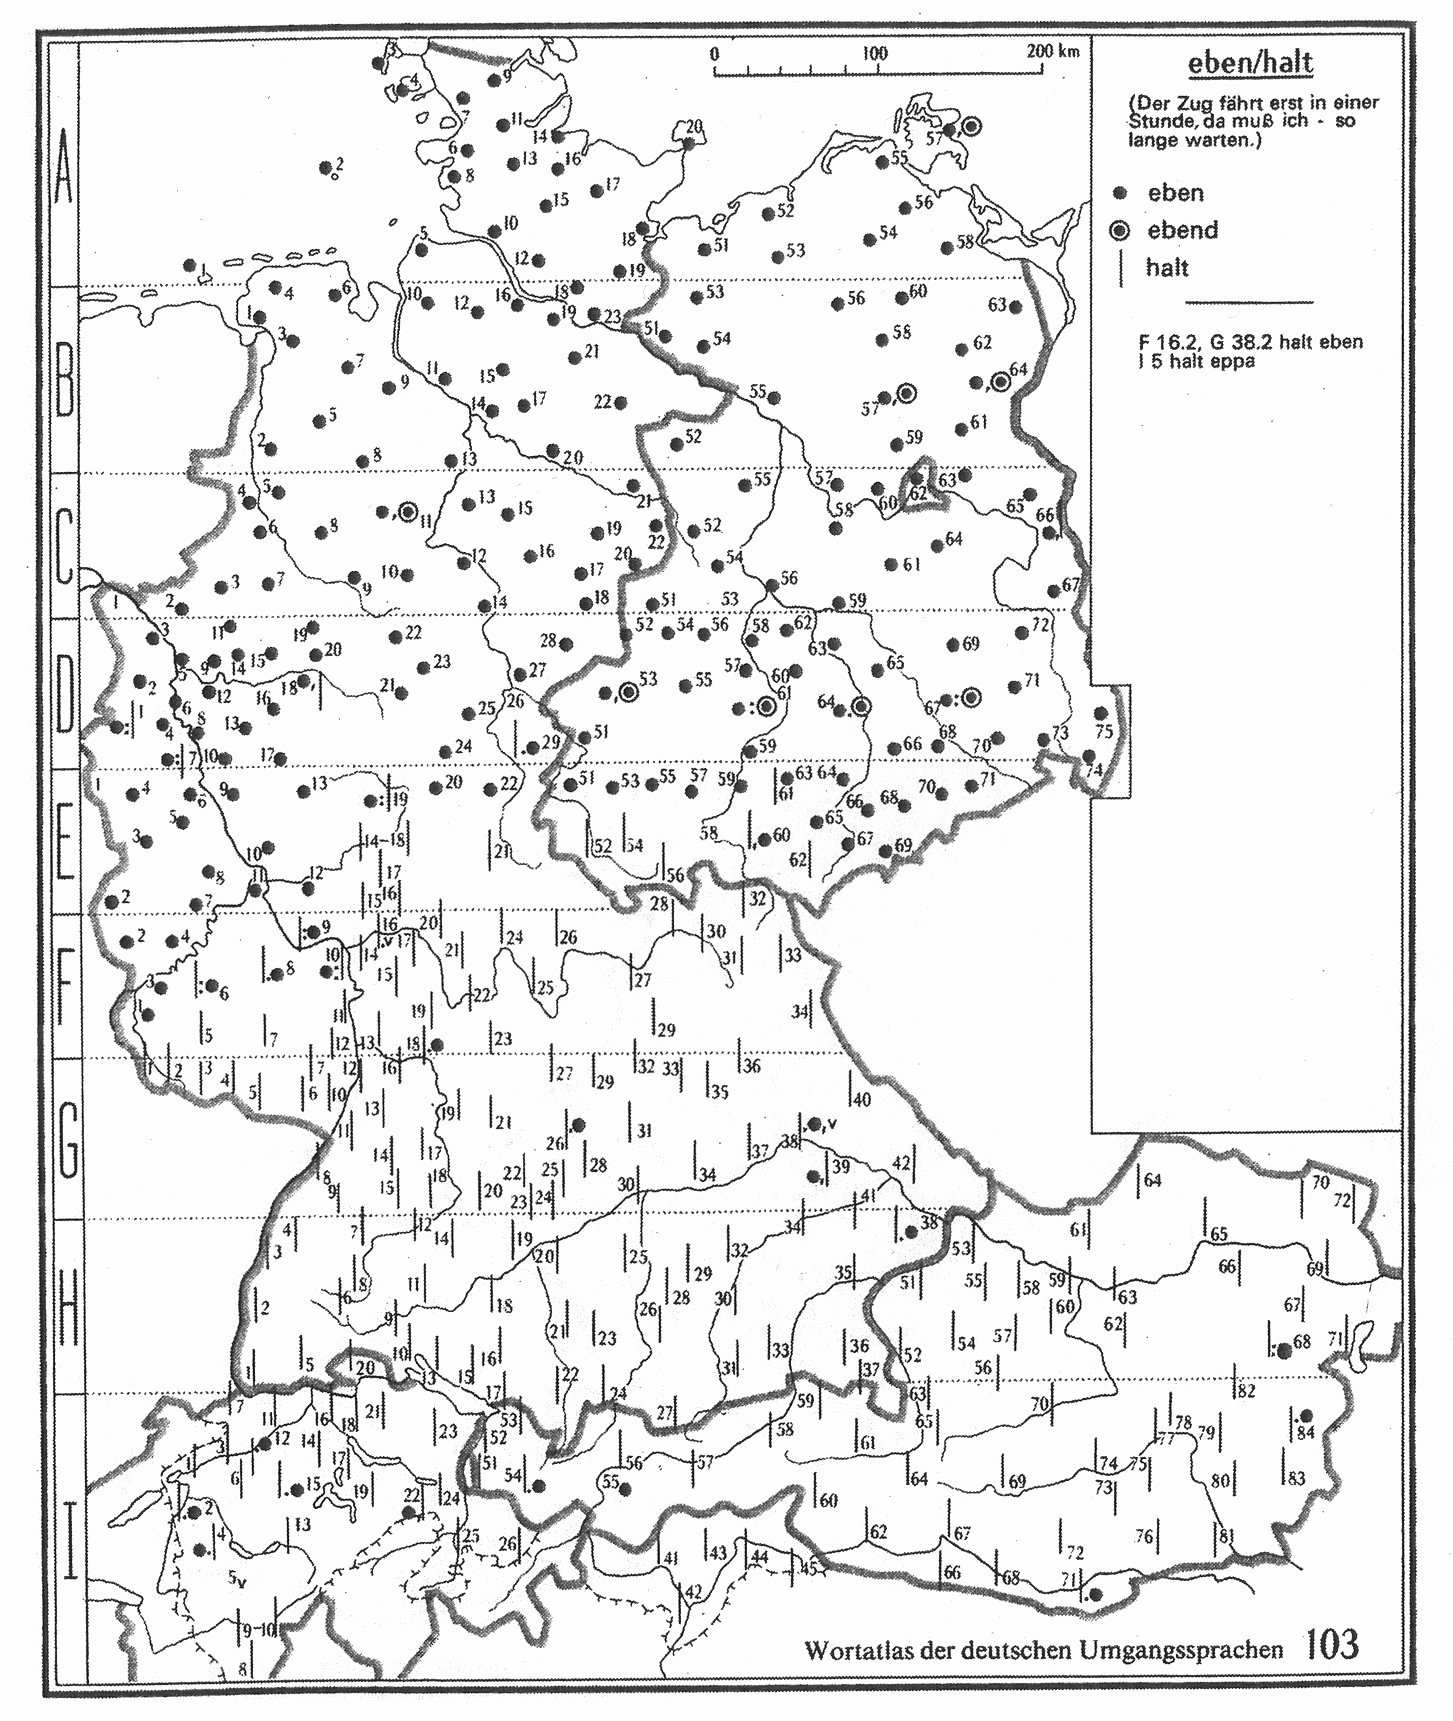
\includegraphics[width=0.7\textwidth]{he1.png}
\caption{Abbildung 1}
\label{Abbildung 1}
\hbox{}\hfill\hbox{\citet[103]{Eichhoff1978}}
\end{figure}	
\noindent
Man sieht hier eine relativ klare Trennung mit \textit{eben} in der oberen Landeshälfte und \textit{halt} in der unteren. Die Grenze verläuft nördlich der Main-Linie. Wenn andere Autoren diese Ergebnisse zusammenfassen, heißt es für die Verteilung in Deutschland, dass \textit{eben} im Norden und \textit{halt} im Süden des Landes auftritt (vgl. z.B. \citealt[212]{Dittmar2000}). Allerdings sieht man an \ref{Abbildung 1} auch, dass \textit{eben} im Süden durchaus vertreten ist, während \textit{halt} nicht im Norden auftritt.

Im Hinblick auf meine eigenen Datenerhebungen, die ich in Abschnitt~\ref{sec:spu} vorstellen werde, ist zu bedenken, dass Eichhoffs Erhebung in den 70er Jahren durchgeführt wurde (1971–1978). D.h. die damaligen Testanten sind heutzutage mindestens 60 Jahre alt (vgl. auch \citealt[2]{Elspass2005}, der hier 2005 von der Eltern- und Großelterngeneration seiner Studenten ausgeht). 

\citet{Elspass2005} berichtet von einer Nacherhebung im Stile von \citet{Eichhoff1978} in Form einer Onlinebefragung, die 2002 stattgefunden hat. Diese Untersuchung ergab die Karte in \ref{Abbildung 2}.

\begin{figure}[h]
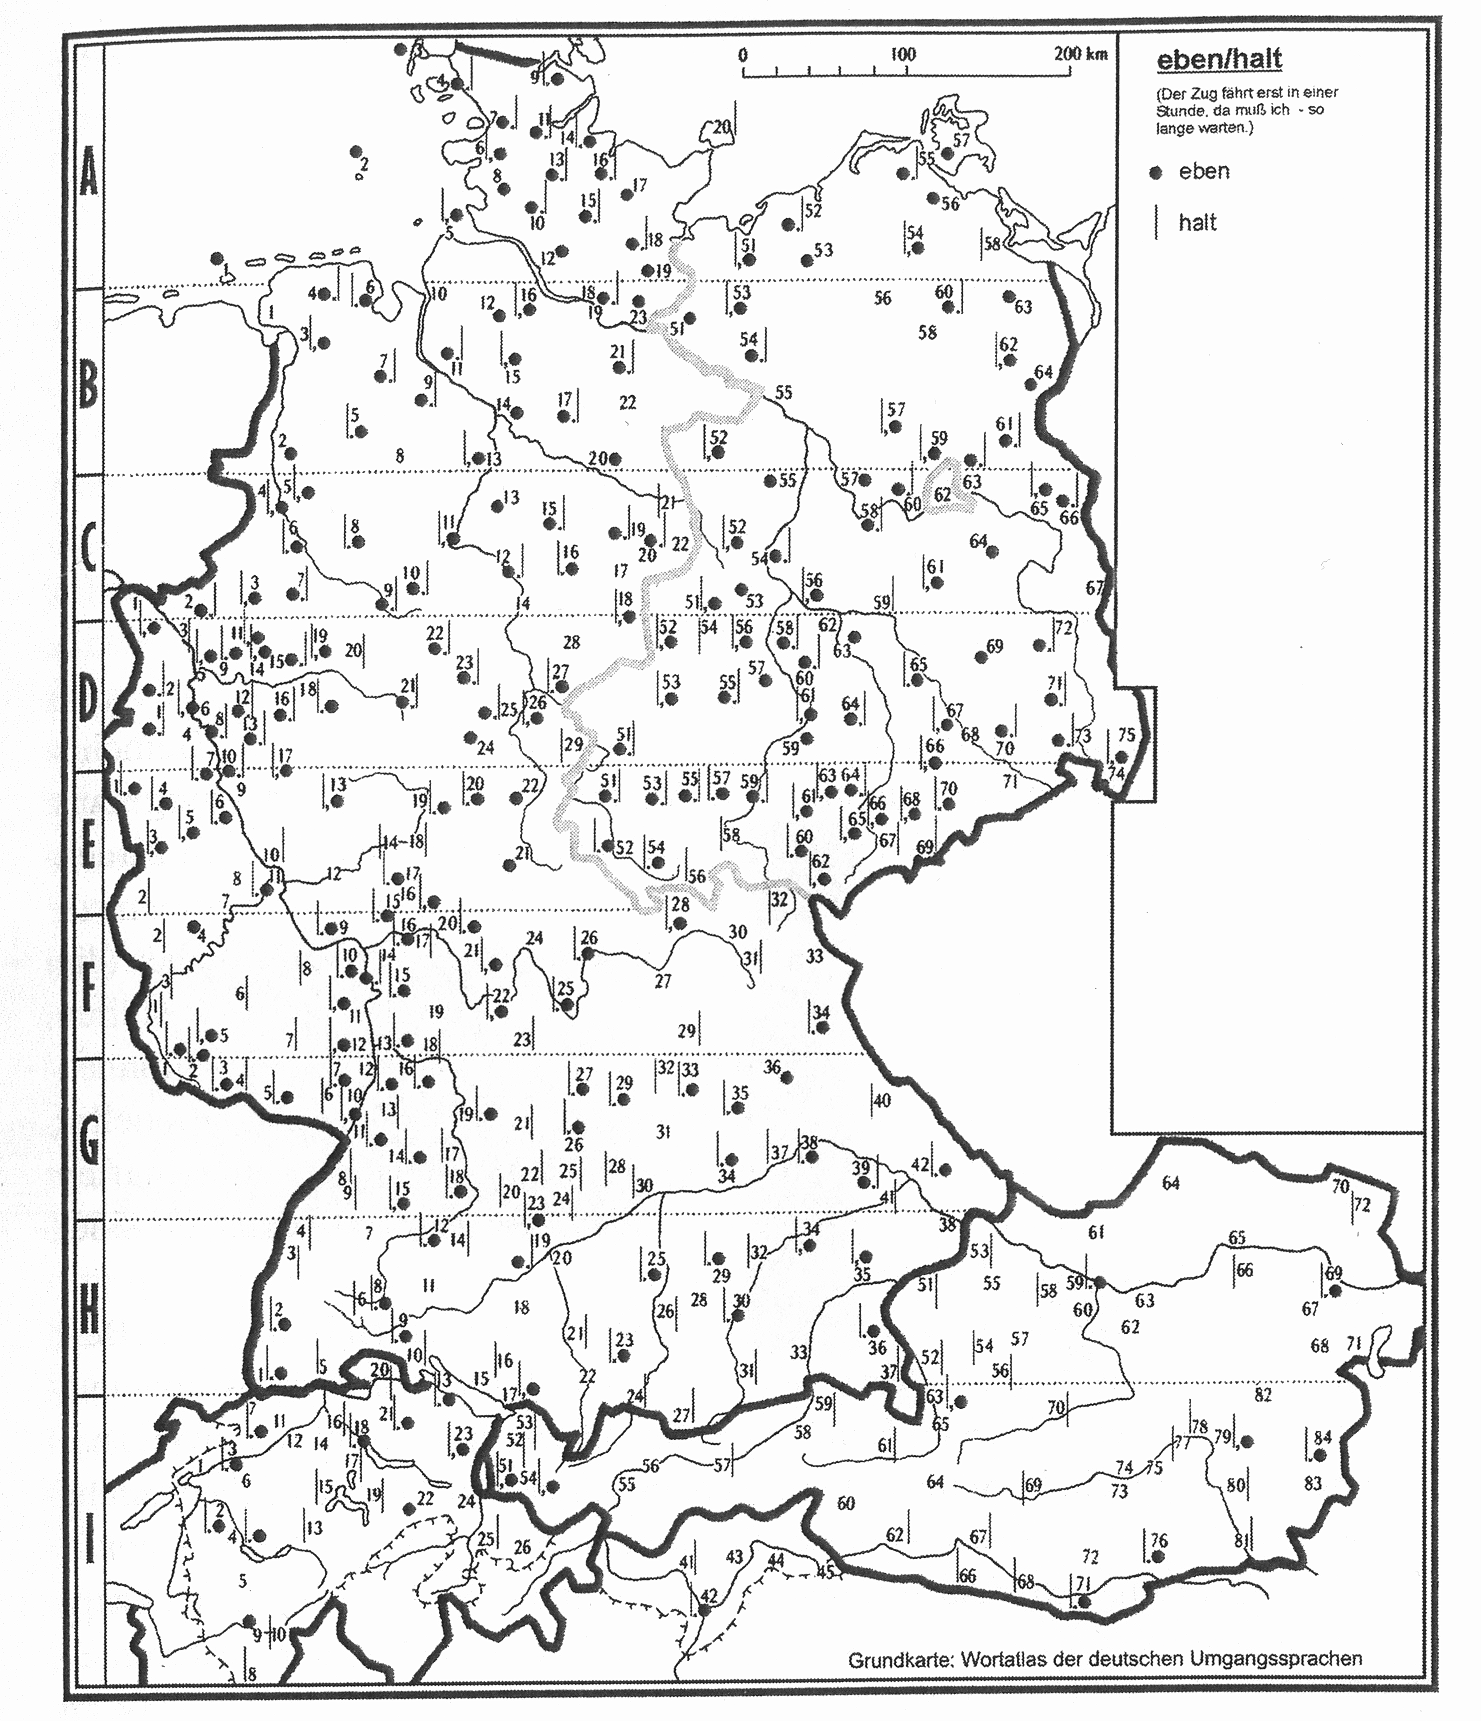
\includegraphics[width=0.7\textwidth]{he2.png}
\caption{Abbildung 2}
\label{Abbildung 2}
\hbox{}\hfill\hbox{\citet[51]{Elspass2005}}
\end{figure}
\noindent
Sie zeigt, dass sich die \textit{halt}-Verwendung in den Norden ausgeweitet hat, sowie dass \textit{eben} (wenn auch weniger) auch in anderen Gebieten auftritt.

Aus diesen Untersuchungen hat man abgeleitet, dass man es bei der Verwendung von \textit{halt} und \textit{eben} mit einem Nord-Süd-Gefälle zu tun hatte, das sich aber abgebaut zu haben scheint. Im Süden Deutschlands (bzw. in der Schweiz und Österreich) existieren \textit{halt} und \textit{eben} bereits zur Zeit der ersten Untersuchungen nebeneinander (wenngleich \textit{halt} nach \ref{Abbildung 1} zu überwiegen scheint $[$s.u. weiteres dazu$]$). Im Norden gab es Zeiten, in denen nur \textit{eben} gebräuchlich war; \textit{halt} hat aber Eingang in den Sprachgebrauch dort gefunden. Für das Gegenwartsdeutsche ist somit davon auszugehen, dass die beiden MPn im gesamten Sprachgebiet nebeneinander existieren. Dies schreiben sogar auch schon Autoren, die in den 80er Jahren auf die erste Untersuchung von Eichhoff blicken (z.B. \citealt[78]{Hartog1982}, \citealt[97]{Dahl1988}, \citealt[124]{Thurmair1989}; vgl. auch \citealt[93]{Autenrieth2002}). Die Etablierung des \textit{halt}-Gebrauchs in der oberen Landeshälfte scheint also in den 80er Jahren eingetreten zu sein.

Ähnliche Verteilungsunterschiede wurden auch für die West-Ost-Achse ange\-nommen. \citet{Protze1997} berichtet von einer Untersuchung aus der zweiten Hälfte der 70er Jahre bis 1980. Es handelt sich um Umfragen wie bei \citet{Eichhoff1977}; (\citeyear{Eichhoff1978}) die in 296 Städten der ehemaligen DDR durchgeführt wurden. Die \textit{eben}/\textit{halt}-Verteilungen, die sich auf der Basis des Testsatzes in (\ref{539}) ergaben, sind in der Karte in \ref{Abbildung 3} dargestellt.

\begin{figure}[h]
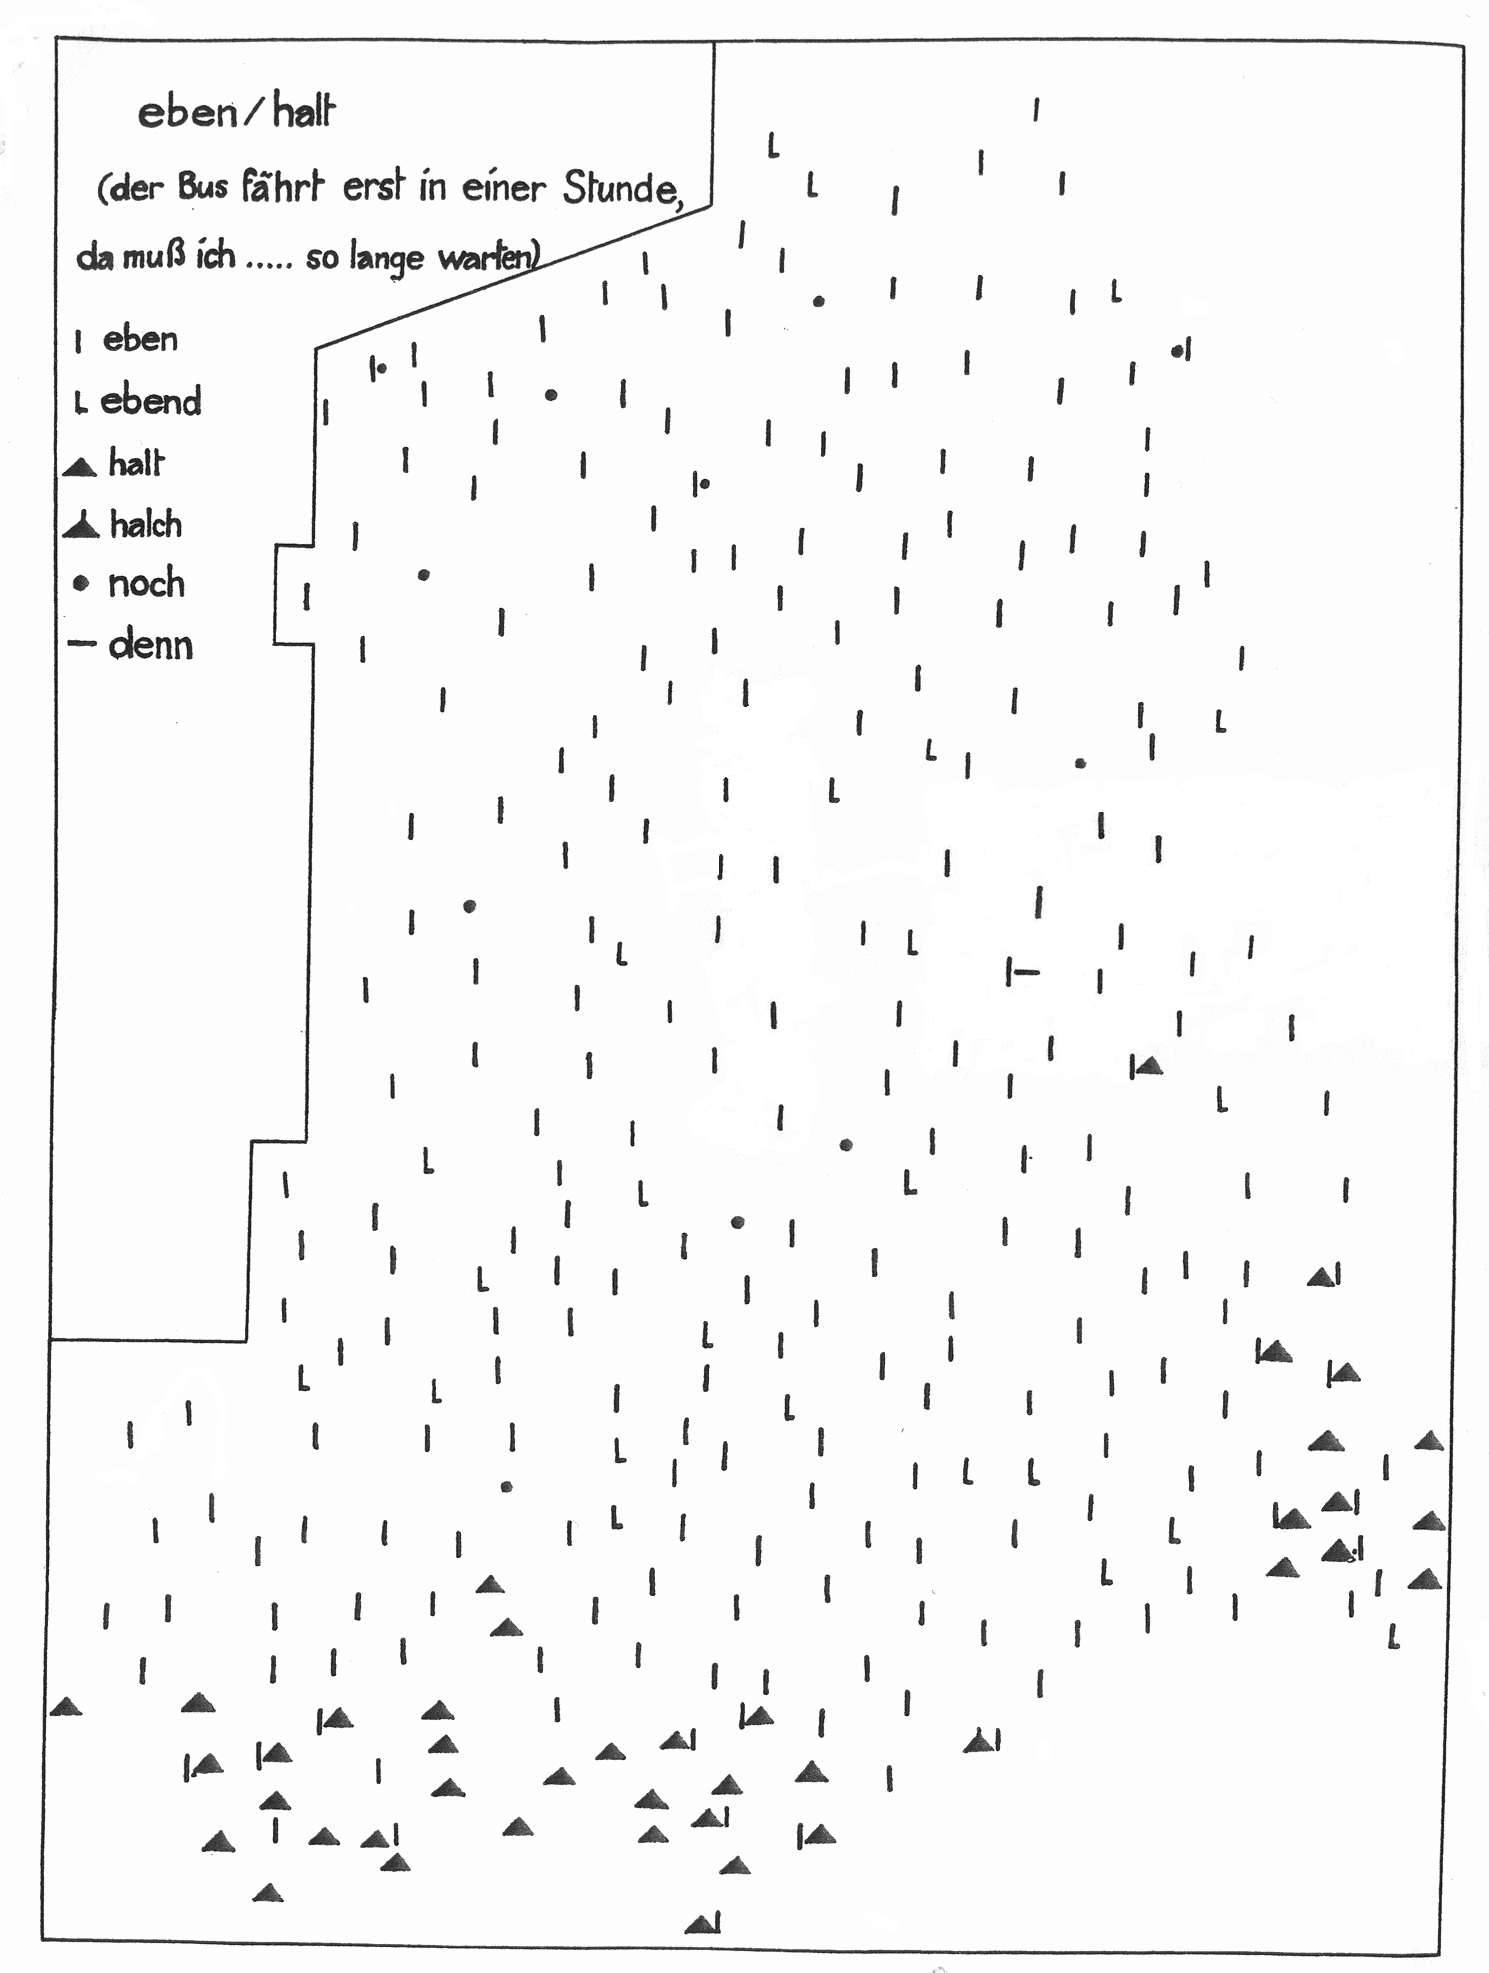
\includegraphics[width=0.5\textwidth]{he3.png}
\caption{Abbildung 3}
\label{Abbildung 3}
\hbox{}\hfill\hbox{\citet[266]{Protze1997}}
\end{figure}

\begin{exe}
	\ex\label{539} 
    Der Bus fährt erst in einer Stunde; da muß ich ... so lange warten. 
    \newline		
	\hbox{}\hfill\hbox{\citet[167]{Protze1997}}    
\end{exe}
Man sieht, dass in den neuen Bundesländern fast flächendeckend \textit{eben} verwendet wurde. Ausnahmen sind Südthüringen, das Vogtland (Südsachsen) und die Oberlausitz (Nord-Ost-Sachsen), wo \textit{halt} als gebräuchlichste Form genannt wurde.

Eine spätere Untersuchung zur unterschiedlichen Verteilung von \textit{halt} und \textit{eben} in Ost- und Westdeutschland findet sich in \citet{Dittmar2000}. Er beschäftigt sich mit den Auswirkungen von Mauerfall und Wiedervereinigung auf den Sprachgebrauch in den neuen Bundesländern. Die Datenbasis sind Interviews in Ost- und Westberlin zwischen 1993 und 1996, in denen die Befragten von ihren persönlichen Erfahrungen mit dem 09.11.1989, der Zeit danach sowie den Auswirkungen der Ereignisse auf ihre aktuelle Situation berichten. Der zentraler Punkt in \citet[213]{Dittmar2000} ist, dass die Verwendung von \textit{halt} vs. \textit{eben} einen soziolinguistischen Grund hat, in dem Sinne, dass \textit{halt} als sozialprestigeträchtig angesehen worden sei. Prinzipiell hätten die Westberliner in den Interviews häufiger \textit{halt} verwendet als die Ostberliner (s.u.). Dazu habe die \textit{halt}-Verwendung nach der \glq Wende \grq {} in Ost-Berlin und den neuen Bundesländern zugenommen. Evidenz für den hohen sozialen Status des \textit{halt}-Gebrauchs und die (daraus resultierende) Anpassung der östlichen an die westliche Sprachgemeinschaft geben metalinguistische Äußerungen wie die folgenden aus \citet[230]{Dittmar2000}.
\begin{exe}
	\ex\label{540} 
		\begin{tabular}[t]{ll} 
 		B & jo also mir' ich zucke auch zusammen eh wenn mit das \textbf{halt} raus-   \tabularnewline
 		 & rutscht;   \tabularnewline
 		I & warum? \tabularnewline
 		B & eh weil ich natürlich ganz genau weiß dieses \textbf{halt} is son marker, den' \tabularnewline
 		& den man eh bewusst setzen kann dass man \textbf{eben} sich integriert oder \tabularnewline
 		& oder dass es \textbf{eben} einfach dass es übernommen wird. \tabularnewline
 		I & wohin? \tabularnewline
 		B &	na in ein' in eine sprachgemeinschaft west;	
  		\end{tabular}				
\end{exe}																	
Dittmar gibt Häufigkeiten für jeden Sprecher zum Gebrauch von \textit{halt} und \textit{eben} in diesen Interviews an. In der Tabelle in (\ref{541}) lässt sich ablesen, dass sowohl die West- als auch die Ostberliner insgesamt häufiger \textit{eben} als \textit{halt} verwenden und dass dieses Gefälle bei den Ostberlinern außerdem stärker ausgeprägt war als bei den Westberlinern.

\begin{exe}
	\ex\label{541} 
		\begin{tabular}[t]{|l|l|l:cx{1pt}l|} 
		\hline
 		& \textit{\textbf{eben}} & \textit{\textbf{ebent}} & \textit{\textbf{eben}} & \textit{\textbf{halt}}   \tabularnewline
 		\hline
 		& & & (\textbf{gesamt}) & \tabularnewline
 		\hline
 		\textbf{31 Ostberliner} & 245 & 372 & 617 & 204 \tabularnewline
 		\hline
 		\textbf{25 Westberliner} & 213 & 96 & 309 & 161 \tabularnewline
 		\hline
  		\end{tabular}			
\end{exe}	
 		\hfill\hbox {\citet[221]{Dittmar2000}}\\
Dieser Eindruck bestätigt sich auch, wenn man die Verwendung bei den einzelnen Sprechern betrachtet. Von den 31 Ostberlinern verwenden 17, also mehr als die Hälfte, \textit{halt} gar nicht. Es gibt nur fünf Sprecher, die häufiger \textit{halt} als \textit{eben} gebrauchen, und lediglich drei, die sowohl \textit{eben} als auch \textit{halt} etwa gleich häufig verwenden. Unter den 25 Westberlinern befinden sich acht Sprecher (ca. ein Drittel), die \textit{halt} gar nicht äußern, fünf verwenden \textit{halt} häufiger als \textit{eben} und bei sechs weiteren Sprechern finden \textit{halt} und \textit{eben} etwa gleich häufig Verwendung (vgl. die Daten in \citealt[121-122]{Dittmar2000}).

Fasst man die Ergebnisse der hier skizzierten Untersuchungen zusammen, lässt sich – bis in die 70er Jahre rückblickend – sagen, dass \textit{halt} und \textit{eben} einmal regional verteilt waren: Das Süddeutsche kennt seit dieser Zeit sowohl \textit{halt} als auch \textit{eben}, das Nord- und Ostdeutsche verwendete \textit{eben} (mit einigen \textit{halt}-Flecken in Ostdeutschland). Dazu ist eine Bewegung von \textit{halt} von Süden nach Norden und von Westen nach Osten zu verzeichnen. Für das heutige Deutsch ist davon auszugehen, dass im gesamten deutschen Sprachgebiet \textit{halt} und \textit{eben} nebeneinander existieren.

\subsection{Zur Validität der dialektalen Erhebungen}
\label{sec:val}
Bei den hier skizzierten dialektalen Annahmen zu \textit{halt} und \textit{eben} handelt es sich um Aspekte, die sich bei dieser Thematik etabliert haben und die deshalb immer wieder in Arbeiten angeführt werden. Gerade deshalb halte ich es für wichtig, auch auf einige Kritikpunkte und fragliche Basen von Aussagen hinzuweisen, die z.T. auch bereits in anderen Arbeiten angeführt worden sind. Sie betreffen die Art der Fragestellung, die Auswertung und Darstellung der Ergebnisse, die Auswahl der Testsätze sowie die Repräsentativität der Ergebnisse.

Beispielsweise kritisiert \citet[16-17]{Elspass2005} mit \citet[174-178]{Hentschel1986} die Fragestellung von \citet{Eichhoff1978}, der danach fragte, ob \textit{halt}, \textit{eben} oder ein anderer Ausdruck in (\ref{542a}) verwendet werde.

\begin{exe}
	\ex\label{542a} 
 Der Zug fährt erst in einer Stunde, da muß ich .......... so lange warten.
\end{exe}																
Da es im Süddeutschen auch dialektale Formen gibt (wie \textit{ebe}, \textit{eaba}), ist es \citet[174]{Hentschel1986} zufolge unplausibel, dass der Gebrauch von \textit{halt} derart überwiegen soll. Sie nimmt an, dass \textit{halt} im Süden als mundartlicher gilt. Da die Testanten wussten, dass es sich um eine dialektale Erhebung handelt und dass \textit{halt} im Norddeutschen bzw. generell im Standarddeutschen unüblich ist, hätten sie sich (da sie sich für eine Form entscheiden mussten) für \textit{halt} entschieden, obwohl sie \textit{eben} gleichermaßen kannten. Unter dieser Sicht wären also die Art der Abfrage und die Umstände, unter denen sie stattfand, mit dafür verantwortlich, dass \textit{eben} auf der Karte in \ref{Abbildung 2} im süddeutschen Raum unterrepräsentiert zu sein scheint. Neben dem Bewusstsein um den dialektalen Status von \textit{halt}, führt \citet[176]{Hentschel1986} ebenfalls die Möglichkeit an, dass die Befragten sich für \textit{halt} entschieden, weil es positivere Konnotationen (wie \textit{weich}, \textit{warm}) aufweise. Um derartige mögliche Störfaktoren zu umgehen, beabsichtigte \citet{Elspass2005} eine Fragestellung, die die Testanten nicht zur Auswahl einer der beiden Formen zwang. Seine Formulierung lautete deshalb: \glqq Setzt man \textit{halt} oder \textit{eben}, beides oder einen anderen Ausdruck ...?\grqq{}  (\citealt[17, Fn 41]{Elspass2005} 17). Doch wie er selbst bemerkt, ist diese Version nicht eindeutig, da er mit \textit{beides} nicht auf die Nennung der Kombination der beiden MPn abzielen wollte (d.h. \textit{halt eben} oder \textit{eben halt}), sondern auf die Gleichwertigkeit der beiden Formen. Auch diese Formulierung ist nicht vollständig geglückt.

Wie die Art der Befragung bzw. die anschließende Aufarbeitung in Form der Karten Ergebnisse beeinflussen kann, zeigt auch die neueste Untersuchung zur Thematik von Elspaß \& Möller (2012) (unter http://www.atlas-alltagssprache.de/\\runde-9/). Betrachtet man die Karte in Abbildung \ref{Abbildung 4}, gewinnt man den Eindruck, \textit{eben} werde in Süddeutschland, Österreich und der Schweiz überhaupt nicht verwendet.
\begin{figure}[h]
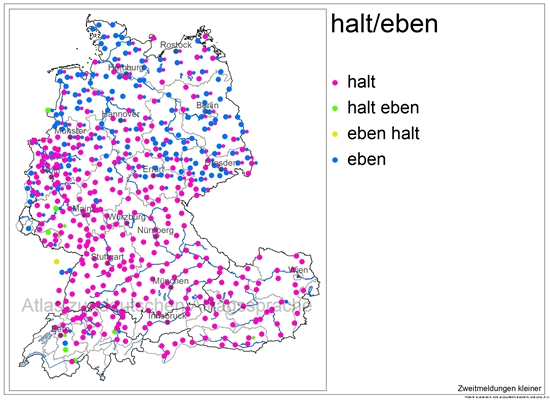
\includegraphics[width=0.7\textwidth]{he4.png}
\caption{Abbildung 4}
\label{Abbildung 4}
\hbox{}\hfill\hbox{(http://www.atlas-alltagssprache.de/halt-eben/)}
\hbox{}\hfill\hbox{(eingesehen am 05.05.2014)}
\end{figure}
\noindent																                       										
Dies verwundert, zumal dies in keiner Weise den Ergebnissen/Darstellungen der älteren Untersuchungen (weder \citealt{Eichhoff1978} noch \citealt{Elspass2005}) entspricht. Die Lösung dieses überraschenden Ergebnisses präsentieren die Autoren selbst:			
\begin{quotation}														                       										Zur Kartierung: Bei verschiedenen Antworten aus ein und demselben Ort ist die häufiger genannte Variante kartiert, in vielen Karten daneben auch (kleiner) die seltener genannte Variante, sofern sie mehr als 35\% der Nennungen ausmacht. Bei gleich häufiger Nennung musste nach dem Zufalls\-prinzip entschieden werden, welche Variante als Erst- bzw. Zweitvariante kartiert wurde. In Karten, bei denen die Wiedergabe der Zweitvarianten vor allem zur Verunklarung der regionalen Unterschiede geführt hätte, wurde der Übersichtlichkeit zuliebe darauf verzichtet. Insofern erscheinen die Unterschiede hier – gegenüber dem tatsächlichen \glqq durchschnittlichen\grqq{} Gebrauch – etwas stärker betont; dies ergibt sich aber auch schon allein aus der Art der Befragung.
\hfill\hbox{(eingesehen am 05.05.2014)}
\newline
\hbox{}\hfill\hbox{(http://www.atlas-alltagssprache.de/halt-eben)}
\end{quotation}
Wieder ist also deutlich zu sehen, dass das Ergebnis (diesmal vornehmlich durch die Art der Auswertung) verzerrt, und zwar in diesem Fall überzeichnet, wird.

Einen weiteren Aspekt gilt es in der Darstellung aus \citet{Dittmar2000} zu berücksichtigen. Er weist selbst darauf hin, dass seine Ergebnisse nur bedingt aussagekräftig sind, da einerseits die Informantenzahl verschieden (25 West- vs. 31 Ostberliner) und andererseits die Interviewausschnitte unterschiedlich lang waren (vgl. \citealt[222]{Dittmar2000}). Vor diesem Kritikpunkt ist Dittmars Ergebnis, dass mehr Westberliner \textit{halt} überhaupt benutzen, allerdings auch umso bedeutender, da die Interviews mit den Ostberlinern sogar länger sind und sie somit mehr Möglichkeiten hatten, \textit{halt} zu verwenden (wenn sie es überhaupt verwenden) (vgl. \citealt[222]{Dittmar2000}).

Ein letzter Aspekt, der in den Untersuchungen von Eichhoff, Elspaß und Protze nicht genügend Beachtung findet, ist die Frage, ob in dem einen (!) vorgegebenen Testitem tatsächlich \textit{halt} und \textit{eben} gleichermaßen verwendet werden können. Ich möchte meine konkreten Bedenken auf Abschnitt~\ref{sec:spu} verschieben, um unter Bezug auf meine Bedeutungsmodellierung präziser argumentieren zu können. An dieser Stelle sei aber bereits angemerkt, dass der regionale Charakter (insbesondere bei prinzipieller Bekanntheit beider Formen) wohl nur nachweisbar ist, wenn die beiden MPn in der vorliegenden Äußerung tatsächlich beide gleichermaßen plausibel auftreten können. Im Rahmen ihrer Analyse der Interpretation von \textit{halt} und \textit{eben} bezweifelt auch schon \citet[174]{Hentschel1986} dies in Bezug auf Eichhoffs Testsatz. Nach der Autorin ist \textit{halt} emotionaler konnotiert als \textit{eben} und der Kontext in (\ref{542a}) lege diese Lesart nahe.

\subsection{Die Bedeutung von \textit{halt} und \textit{eben}}
\label{sec:bedhe}
Wenn Autoren annehmen, dass es die zwei Formen \textit{halt} und \textit{eben} deshalb gibt, weil sie regional verteilt sind, geht diese Sicht damit einher, dass sie ihre Bedeutung und Verwendung für identisch halten (vgl. z.B. \citealt[10]{Becker1978}, \citealt[358]{Luetten1977}, \citealt[81]{Bublitz1978}, \citealt[202]{Karagjosova2004}). Es wird dann eine Bedeutung für \textit{eben} angegeben, die auf \textit{halt} gleichermaßen zutreffen soll. Wenige Autoren beschäftigen sich hingegen mit der Bedeutung von \textit{halt} und betrachten es in Differenz zu \textit{eben}. Die Bedeutung, die von ersteren Autoren sowohl für \textit{halt} als auch für \textit{eben} angesetzt wird, ist dann in der Regel diejenige, die Autoren, die sich für einen Unterschied zwischen den beiden Partikeln aussprechen, für \textit{eben} formulieren.

\subsubsection{Gemeinsamkeiten}
Die Illokutionstypen, in denen \textit{halt} und \textit{eben} auftreten können, sind Assertionen \is{Assertion} und \is{Direktiv} Direktive.\footnote{Die beiden Partikeln können auch in verschiedenen Nebensatztypen auftreten, vor allem \textit{halt} scheint hier
sehr frei verwendet werden zu können (z.B. Kausalsätze, Konditionalsätze, Temporalsätze, Instrumentalsätze $[$zu einem Überblick vgl. \citealt[202-203]{Hentschel1986}$]$). Ich gehe auf die Nebensatzverwendungen an dieser Stelle nicht ein, betrachte in Abschnitt~\ref{sec:rs} allerdings ihr Auftreten in Relativsätzen sehr detailliert.}

\begin{exe}
	\ex\label{542} Assertion\\
	A: Peter sieht sehr schlecht aus. (= q)\\
	B: Er war \textbf{eben}/\textbf{halt} lange krank gewesen. (= p)		
\end{exe}	

\begin{exe}
	\ex\label{543} Direktiv\\
	A: Ich schaffe es nicht bis morgen! (= q)\\
	B: Arbeite eben/halt schneller! (= p)	
	\hfill\hbox{\citet[340/215]{Karagjosova2004}} 	
\end{exe}				    
Die klassischen Merkmale, die in Beschreibungen dieser zwei Partikeln genannt werden (vgl. auch \citealt[150-152]{Mueller2016a}; \citeyear[165-169]{Mueller2016b}, \citeyear[239-243]{Mueller2017a}), sind zum einen die \textit{Rückorientierung} von \textit{eben}/\textit{halt}-Äußerungen und zum anderen der Aspekt der \textit{Kategorizität}. Die Eigenschaft der Rückorientierung (vgl. z.B. \citealt[98, 224]{Dahl1988}, \citealt[120, 125-126]{Thurmair1989}, \citealt[340]{Karagjosova2003}; \citeyear[208]{Karagjosova2004}) zeigt sich generell darin, dass diese MP-Äußerungen immer Reaktionen auf eine vorausgehende Äußerung oder Situation sind. Wie in Abschnitt~\ref{sec:zugang} in Kapitel~\ref{chapter:hintergrund} erläutert, sind MPn prinzipiell reaktiver Natur. Diese Eigenschaft trifft auf \textit{halt} und \textit{eben} aber umso mehr zu, da die Bedingung bzw. das Begründende vorerwähnt sein muss. Sie können nicht redeeinleitend verwendet werden und eignen sich nicht zum Themenwechsel. Konkreter wird für diese Relation angenommen, dass die MP-Äußerung und eine andere Äußerung in einem kausalen Verhältnis \is{kausale Relation} zueinander stehen oder eine Bedingungs-Folge-Relation \is{Bedingungs-Folge-Relation} vorliegt (vgl. z.B. \citealt[40]{Weydt1969}, \citealt[101, 288 Fn 60, 125]{Dahl1988}, \citealt[121]{Helbig1990}, \citealt[67]{Koenig1997}). 

In (\ref{542}) beispielsweise ist das Kranksein die Begründung für das schlechte Aussehen. Die MP-Äußerung gibt hier den Grund für den Inhalt der vorausgehenden Äußerung an (vgl. (\ref{544})).

\begin{exe}
	\ex\label{544} Weil er lange krank gewesen ist (= p), sieht Peter schlecht aus (= q).		
\end{exe}
Mit dieser Funktion der \textit{eben}/\textit{halt}-Äußerung ist gut verträglich, dass einer solchen Äußerung gerne eine Frage nach dem Grund vorweggeht (vgl. (\ref{545}), (\ref{546}) (vgl. \citealt[121]{Thurmair1989})).
\begin{exe}
	\ex\label{545} 
	Hans: Warum sind nur die Frauen so hinter dir her?\\
	Peter: Ich bin \textbf{eben} unwiderstehlich.
	\hfill\hbox{\citet[121]{Thurmair1989}} 	
\end{exe}	

\begin{exe}
	\ex\label{546} 
	Warum bist du denn so fad?\\
	Ich bin \textbf{halt} krank.	
	\hfill\hbox{\citet[312]{Schlieben-Lange1979}} 	
\end{exe}	
Eine Äußerung ohne Partikel ist hier situativ unangemessen und das Auftreten einer kausalen Konjunktion ist in diesem Fall notwendig (vgl. (\ref{547})).

\begin{exe}
	\ex\label{547} 
	Hans: Warum sind nur die Frauen so hinter dir her?\\
	Peter: ?Ich bin unwiderstehlich./Weil ich unwiderstehlich bin.	
	\newline
	\hbox{}\hfill\hbox{\citet[121]{Thurmair1989}} 	
\end{exe}
Bei den \glq Begründungen\grq {} muss es sich dabei nicht um tatsächliche Begründungen handeln. In (\ref{548}) und (\ref{549}) liegen keine oder nur sehr oberflächliche Begründungen vor (vgl. \citealt[322]{Troemel-Ploetz1979}).

\begin{exe}
	\ex\label{548} 
	Wieso muss man denn hier fünf Fragebögen ausfüllen? – Das ist \textbf{eben} so.	
	\newline
	\hbox{}\hfill\hbox{\citet[312]{Schlieben-Lange1979}} 	
\end{exe}	
\begin{exe}
	\ex\label{549} 
	Warum esst ihr denn mit Stäbchen? – Das gefällt uns \textbf{eben}.
	\newline
	\hbox{}\hfill\hbox{\citet[322]{Troemel-Ploetz1979}} 	
\end{exe}																	              
Ein Beispiel für eine Bedingungs-Folge-Relation findet sich in (\ref{550}).

\begin{exe}
	\ex\label{550} 
	Evi: Du, das ist ganz blöd heute, ich hab noch so wahnsinnig viel zu tun. 
	\newline
	\hbox{}\hfill\hbox{(= q)}\\
	Pit: Gut, komm ich \textbf{halt}/\textbf{eben} morgen. (= p) So dringend ist es ja nicht.
	\newline
	\hbox{}\hfill\hbox{nach \citet[122]{Thurmair1989}} 	
\end{exe}

\begin{exe}
	\ex\label{551} 
	\glq Wenn du so viel zu tun hast (= q), dann komme ich morgen (= p).\grq {} 	
\end{exe}
Assertive Fälle können sowohl den Grund (vgl. (\ref{542})) als auch (wie in (\ref{550})) die Folge angeben. In Direktiven scheint mir der MP-Teilsatz immer die Folge auszumachen (vgl. (\ref{543}) und (\ref{552})).

\begin{exe}
	\ex\label{552} 
	Wenn du es nicht bis morgen schaffst (= q), musst du schneller arbeiten. 
	\newline
	\hbox{}\hfill\hbox{(= p)} 	
\end{exe}
Ein anderes Merkmal, das bei der Charakterisierung von \textit{eben} (und ggf. auch \textit{halt}) angeführt wird, ist das der \textit{Kategorizität}. 

Bei \citet[120-121]{Helbig1990} und \citet[340]{Karagjosova2003} heißt es über \textit{halt} und \textit{eben}, der Sachverhalt werde als \textit{unabänderlich}, \textit{kategorisch} und \textit{Thema beendend} ausgegeben. \citet[80/83]{Autenrieth2002} spricht von \textit{Absolutheit} und \textit{Kategorizität}. \citet[120]{Thurmair1989} schreibt, der Sachverhalt sei \textit{evident} (zu \textit{eben}). In Direktiven entspricht dies dem Verhältnis, dass die Handlung, zu der aufgefordert wird, \textit{offensichtlich} ist und die \textit{einzig mögliche Lösung des Problems} darstellt (vgl. \citealt[122]{Thurmair1989}, vgl. auch \citealt[169]{Hentschel1986}). Wie für alle mit MPn erreichten Effekte gilt auch hier, dass die Bedeutungsmomente \textit{Evidenz} und \textit{Faktum} auch nur vorgegeben sein können. \citet[320-323]{Troemel-Ploetz1979} nimmt für \textit{eben} an, die MP gebe die Proposition als \textit{generell gültig} und als \textit{Faktum} aus. Der Hörer könne die Annahme nicht in Frage stellen oder ihr widersprechen. Weitere Diskussionen würden sich erübrigen. Die Aussage werde als \textit{axiomatisch} dargestellt und die Behauptung somit \textit{immunisiert}. Auch die Auffassung von \citet[130]{Diewald1997} zu \textit{eben}, die Proposition sei \glqq bereits gegeben und aktuell wiederholt\grqq{} fügt sich in dieses Bild ein. \citet{Autenrieth2002} weist anhand von Beispielen der Art in (\ref{553}) darauf hin, dass die Charakterisierung \textit{unabänderlich} ggf. auch zu stark ausfalle, da auf solche Äußerungen eher verwandte, aber schwächere Bedeutungs\-zuschreibungen wie \textit{unspektakulär}, \textit{unproblematisch} und \textit{gewöhnlich} zutreffen würden.

\begin{exe}
	\ex\label{553} 
	(S zeigt Foto)\\
	Und auf DIEsem Foto ist Beates Kuchen dann \textbf{halt}/\textbf{eben} fertig und steht auf dem Tisch.		
	\hfill\hbox{nach \citet[99]{Autenrieth2002}} 
\end{exe}
Es ist auch darauf hingewiesen worden, dass sich die Bedeutungseffekte \textit{Evidenz} und \textit{Kategorizität} ebenfalls auf die Relation und nicht (nur) auf die Proposition der MP-Äußerung beziehen können (vgl. \citealt[99]{Dahl1988}). In (\ref{554}) wird nach Dahls Argumentation (zu \textit{eben} und \textit{halt}) nicht der Sachverhalt, dass der Nachbar Choleriker ist, als kategorisch/axiomatisch ausgegeben, sondern die Relation zwi\-schen den Propositionen (der Nachbar macht Krach und der Nachbar ist Choleriker).

\begin{exe}
	\ex\label{554} 
	A: Unser Nachbar hat heute wieder Krach gemacht.\\
	B: Er ist \textbf{eben} ein Choleriker.		
	\hfill\hbox{nach \citet[98]{Dahl1988}} 
\end{exe}
In (\ref{555}) ist der Zusammenhang bekannt:
\begin{exe}
	\ex\label{555} 
	Wenn jemand Choleriker ist, wird es bei ihm auch manchmal laut.
\end{exe}
Dahl nimmt dazu an, die \textit{eben}-Äußerung wirke \textit{abqualifizierend} (\citeyear[100]{Dahl1988}), in dem Sinne, dass B die Berechtigung der vorausgehenden Äußerung bestreitet. B widerspricht den Erwartungen, die A mit seiner Äußerung ausdrückt. Im Falle einer Assertion wie in (\ref{554}) ist dies die Annahme, dass er B etwas mitteilt, das wissenswert ist. Diese Erwartung wird in (\ref{554}) gestört, weil die Proposition aus As Äußerung ableitbar ist. Parallele Verhältnisse liegen auch in Direktiven wie in (\ref{556}) vor.
\begin{exe}
	\ex\label{556} 
	A: Mein Zahn tut mir weh.\\
	B: Dann geh \textbf{eben} zum Zahnarzt!
	\hfill\hbox{nach \citet[101]{Dahl1988}} 
\end{exe}
A müsste hier selbst zum Schluss der \textit{eben}-Äußerung kommen, da der Zusammenhang in (\ref{557}) bekannt ist.
\begin{exe}
	\ex\label{557} 
	Wenn dein Zahn weh tut, musst du zum Zahnarzt gehen.
\end{exe}
Es besteht kein Grund zum Klagen für A und die Mitteilung von A ist für die Eröffnung eines Problemlösungsszenarios irrelevant. Auch hier bestreitet B die Berechtigung des vorweggehenden Sprechaktes.

Diese Überlegungen stammen aus \citet[98-101]{Dahl1988} und werden in \citet[340]{Karagjosova2003}; (\citeyear[202-220]{Karagjosova2004}) übernommen, um die Bedeutung von \textit{eben} und \textit{halt} in einem formalen Diskursmodell zu erfassen. Da ich auf ihre Bedeutungszuschreibung in Abschnitt~\ref{sec:modellierung} zurückgreifen werde, seien ihre Annahmen an dieser Stelle bereits angeführt.

Auf der Basis der beiden Kriterien a) Rückorientierung und b) Kategorizität fasst die Autorin den Beitrag von \textit{eben} und \textit{halt} folgendermaßen auf: Zum einen ist die Proposition der MP-Äußerung bekannt. Dies kann p oder q sein (s.u.). Zum anderen ist unter den Diskurspartnern die Inferenzrelation p $>$ q (\glq Normalerweise, wenn p, dann q.\grq {}) bekannt. p $>$ q hat in \citet{Asher1991}, auf die sich Karagjosova hier bezieht, den Status \is{defeasible rule} einer \textit{defeasible rule}. Fungiert die \textit{eben}/\textit{halt}-Äußerung als Begründung der vorweggehenden Äußerung wie in (\ref{558}), ist p bekannt sowie die Inferenzrelation p $>$ q.
\begin{exe}
	\ex\label{558} 
	A: Unser Nachbar hat heute wieder Krach gemacht. (= q)\\
	B: Er ist \textbf{eben} ein Choleriker. (= p)
\end{exe}
Über \textit{modus ponens} \is{modus ponens} unter Beteiligung dieser (pragmatischen) Inferenzrelation, an dem nor\-malerweise ein \underline{logischer} Zusammenhang zwischen p und q beteiligt ist, ist abzuleiten, dass auch q bekannt ist (\textit{deafisible modus ponens} \is{deafisible modus ponens} in \citealt[387]{Asher1991}). 

Stellt die MP-Äußerung die Folge in einem Bedingungs-Folge-Gefüge dar wie in (\ref{559}), dreht sich die Inferenzrelation um. D.h. die Relation q $>$ p ist bekannt, ebenso die Proposition p.\footnote{Alternativ bleibt die Inferenzrelation p $>$ q und die MP bezieht sich auf q (und nicht p).}

\begin{exe}
	\ex\label{559} 
	A: Ich schaffe es nicht bis morgen. (= q)\\
	B: Arbeite \textbf{eben}/\textbf{halt} schneller! (= p)
\end{exe}	
Nach As Äußerung sind A und B sich hinsichtlich q einig. (A ist von q aufgrund seiner Äußerung überzeugt, B gibt einen Rat unter den Umständen von q, was auf seine Akzeptanz von q schließen lässt.) Ebenfalls bekannt ist der Zusammenhang zwischen q und p (\glq Wenn du etwas nicht bis zum nächsten Tag schaffst, musst du schneller arbeiten.\grq {}). Wenn q und q $>$ p bekannt ist, ist auch klar, dass zu p geraten wird.

Karagjosova setzt den hier beschriebenen Effekt sowohl für \textit{halt} als auch für \textit{eben} an. Wie eingangs angeführt, gibt es allerdings auch Autoren, die in ihrer Charakterisierung einen Unterschied zwischen den beiden Partikeln machen.

\subsubsection{Unterschiede}
\label{sec:untersch}
\citet[124]{Thurmair1989} geht davon aus, dass die beiden MPn zwar eine ähnliche Bedeutung haben, es sich aber nicht um Synonyme handelt. Auch \citet[254]{Dahl1988} schreibt schon, \glqq daß es sich eher um funktionale Ähnlichkeit als Äquivalenz\grqq{}  handelt. Eines der Argumente für diese Annahme ist bei \citet{Thurmair1989}, dass \textit{eben} und \textit{halt} nicht beliebig austauschbar sind. So gibt es Kontexte, in denen \textit{eben} im Gegensatz zu \textit{halt} nicht gut stehen kann (vgl. (\ref{5600}) und (\ref{561})).\footnote{Ein Gutachter weist korrekterweise darauf hin, dass ein Beispiel wie (\ref{5600}) zeigt, dass die beteiligte Begründung nicht einer vorher explizit genannten Proposition gelten muss, sondern eine \textit{halt}-/\textit{eben}-Äußerung sich auch auf eine Implikatur der Vorgängeräußerung beziehen kann. In (\ref{5600}) werde nicht die Proposition dass der Adressat seine Freunde mitbringen kann begründet, sondern der durch \textit{schon} ausgedrückte Vorbehalt gegenüber weiteren Gästen.}

\begin{exe}
	\ex\label{5600} Du kannst deine Freunde schon mitbringen.
		\begin{xlist}	
			\ex\label{560a} Wir haben \textbf{halt} kein Bier mehr.
			\ex\label{560b} *Wir haben \textbf{eben} kein Bier mehr.
		\end{xlist}
\end{exe}

\begin{exe}
	\ex\label{560} Monika will Hans um einen Gefallen bitten, zögert aber, ihn anzurufen. Nach einiger Zeit sagt ihre Freundin.
		\begin{xlist}	
			\ex\label{560a} Jetzt ruf den Hans \textbf{halt} an!
			\ex\label{560b} *Jetzt ruf den Hans \textbf{eben} an!
			\hfill\hbox {\citet[124]{Thurmair1989}}
		\end{xlist}
\end{exe}
Umgekehrt sind ihrer Ansicht nach schwieriger Fälle zu finden, in denen \textit{eben} angemessen ist und \textit{halt} unpassend erscheint. Thurmair gibt die Beispiele in (\ref{561}) und (\ref{562}).

\begin{exe}
	\ex\label{561} 
		\begin{xlist}	
			\ex\label{561a} Der Wal ist \textbf{eben} ein Säugetier.
			\ex\label{561b} ?Der Wal ist \textbf{halt} ein Säugetier.
		\end{xlist}
\end{exe}
\begin{exe}
	\ex\label{562} 
		\begin{xlist}	
			\ex\label{562a} Der Krieg ist \textbf{eben} unmoralisch.
			\ex\label{562b} ?Der Krieg ist \textbf{halt} unmoralisch.
			\hfill\hbox {\citet[124]{Thurmair1989}}
		\end{xlist}
\end{exe}
Und auch wenn beide Partikeln in einem Kontext prinzipiell stehen können (vgl. (\ref{563}), (\ref{564})), geht das Auftreten der ein oder anderen Partikel der Autorin zufolge mit einem Interpretationsunterschied einher.

\begin{exe}
	\ex\label{563} 
		\begin{xlist}	
			\ex\label{563a} Männer sind \textbf{eben} so.
			\ex\label{563b} Männer sind \textbf{halt} so.
		\end{xlist}
\end{exe}
\begin{exe}
	\ex\label{564} Ich hab dich doch gewarnt. 
		\begin{xlist}	
			\ex\label{564a} Horrorvideos sind \textbf{eben} grausam.	
			\ex\label{564b} Horrorvideos sind \textbf{halt} grausam.
			\hfill\hbox {\citet[124]{Thurmair1989}}
		\end{xlist}
\end{exe}
Eine \textit{halt}-Äußerung wirke im Vergleich zu einer \textit{eben}-Äußerung abgeschwächter und weniger apodiktisch (vgl. \citealt[125]{Thurmair1989}, vgl. auch schon \citealt[309]{Schlieben-Lange1979}). Wie oben erläutert, zeigen \textit{halt} und \textit{eben} hinsichtlich des Kriteriums des Rückbezugs dasselbe Verhalten. Im Falle von \textit{halt} ist der Sachverhalt (bzw. die Relation) nicht evident/kategorisch/die einzige Möglichkeit, sondern nur plausibel. Die \textit{halt}-Äußerung ist eine plausible Erklärung/Begründung für den Vorgängerbeitrag oder eine plausible Folge aus diesem. Im Falle einer \textit{halt}-Begründung/Erklärung sind alternative Begründungen zugelassen. Der Sprecher vertritt lediglich die von ihm präsentierte Erklärung. Insgesamt wirken \textit{halt}-Assertionen somit abgeschwächter im Vergleich zu \textit{eben}-Assertionen. \textit{Halt}-Auffor\-derungen, \is{Aufforderung} die die Folge aus dem zuvor gesagten darstellen, sind schwächer als \textit{eben}-Aufforderungen. Sie präsentieren nicht apodiktisch die einzig denkbare Lösung, sondern es handelt sich aus Sprechersicht um eine plausible Lösung für das Problem aus dem Vorgängerbeitrag (vgl. \citealt[125-126]{Thurmair1989}, vgl. auch \citealt[316]{Schlieben-Lange1979}, \citealt[74-75]{Hartog1982}, \citealt[235]{Meibauer1994}, \citealt[312]{Rost-Roth1998}, \citealt[98]{Autenrieth2002}).

Unter der Annahme dieses Unterschieds in der Interpretation von \textit{eben}- und \textit{halt}-Äußerungen leitet \citet{Thurmair1989} die Beispiele aus (\ref{560}) und (\ref{561}), in denen die beiden MPn situativ nicht gleichermaßen angemessen sind, auf die folgende Art ab: Sie argumentiert, dass \textit{eben} dann inakzeptabel ist, wenn Alternativen relevant sind und anerkannt werden. In Beispielen der Art in (\ref{560}) und (\ref{561}) stellt der Sachverhalt der MP-Äußerung eine plausible Begründung dar, der Sprecher bzw. der Adressat handelt aber nicht danach. In (\ref{560}) ist es beispielsweise plausibel für den Sprecher, dass, wenn man kein Bier mehr hat, man nicht weitere Gäste einlädt. Dies scheint aber nicht der einzige Zusammenhang zu sein: Wenn dies der einzige denkbare Zusammenhang wäre, könnte er die Freunde schließlich nicht zulassen. Ist die MP-Äußerung die Folge wie im Falle der Aufforderung in (\ref{561}), handelt es sich bei der Handlung, zu der geraten wird, um eine plausible, aber wiederum nicht einzig mögliche Lösung. Den Gesprächspartner anzurufen, ist \underline{eine} Möglichkeit, es ist aber nicht die einzige. Aus dem Kontext ist bekannt, dass der Vorschlag gerade nicht evident ist, da der Adressat genau diese Handlung nicht favorisiert (vgl. \citealt[127]{Thurmair1989}).

In Abschnitt~\ref{sec:modellierung} werde ich erläutern, wie sich diese Fälle in meine Bedeutung\-smodellierung fügen. Die entscheidende Erkenntnis von Thurmair an dieser Stelle, die es m.E. bei jeder Modellierung des Beitrags von \textit{halt}- und \textit{eben}-Äußerungen zu berücksichtigen gilt, ist, dass sich Beispiele finden lassen, in denen \textit{halt} stehen kann, in denen das Auftreten von \textit{eben} aber hingegen nicht angemessen ist. Es handelt sich um Situationen, in denen nicht von Evidenz/Kategorizität, sondern schwächer von Plausibilität auszugehen ist. Umgekehrt ist \textit{halt} dann nicht passend, wenn der ausgedrückte Sachverhalt evident ist. Es ist in diesem Fall nicht angemessen, Alternativen offen zu halten; \textit{halt} ist in diesem Sinne dann zu schwach. Es scheint äußerst unwahrscheinlich, dass nur der Sprecher davon ausgeht, dass der Wal ein Säugetier oder Krieg unmoralisch ist (vgl. (\ref{560}) und (\ref{561})). In Äußerungen dieser Art ist somit nur \textit{eben} zu verwenden. Die Fälle, in denen das Auftreten von \textit{halt} im Gegensatz zu \textit{eben} unangemessen ist, sind allerdings sehr selten (vgl. \citealt[128]{Thurmair1989}).

Die MP \textit{eben} lässt sich folglich in der Regel durch \textit{halt} ersetzen. Der umgekehrte Austausch ist hingegen nicht immer möglich (vgl. \citealt[128]{Thurmair1989}, \citealt[392]{Ickler1994}). Wenn \textit{eben} (mit Thurmair, s.o.) Evidenz anzeigt und \textit{halt} Plausibilität, sind die obigen Verhältnisse folgendermaßen zu erklären: Ein evidenter Sachverhalt ist auch plausibel, eine plausible Sachlage ist aber nicht notwendigerweise evident. In diesem Sinne schließt die Bedeutung von \textit{eben} die Bedeutung von \textit{halt} ein, der Beitrag von \textit{halt} schließt aber nicht den Beitrag von \textit{eben} ein (vgl. \citealt[128]{Thurmair1989}). Ich greife diese Zusammenhänge zu einem späteren Zeitpunkt der Betrachtung wieder auf. Sie sind zentral für meine Argumentation in Abschnitt~\ref{sec:impli}.

\section{Modellierung im Diskursmodell}
\label{sec:modellierung}
Ich bilde die Interpretation der MPn in dieser Arbeit ab, indem ich ihren Diskursbeitrag im Rahmen des formalen Diskursmodells aus \citet{Farkas2010} be\-schreibe. Im Falle von \textit{eben} und \textit{halt} baue ich dabei auf Annahmen und die Analyse von \citet{Karagjosova2003}; (\citeyear{Karagjosova2004}), die ebenfalls mit einem formalen Diskurs\-modell arbeitet. Im Gegensatz zu Karagjosova gehe ich allerdings von einem Unterschied zwischen \textit{eben} und \textit{halt} aus. 

\subsection{Direktive im Diskursmodell}
\label{sec:dirdm}
In der Form, wie von \citet{Farkas2010} entworfen, kann das Diskursmodell (vgl. Abschnitt~\ref{sec:diskursmodell}, Kapitel~\ref{chapter:hintergrund} für eine ausführliche Darstellung) nur Assertionen und E-Fragen erfassen. Da \textit{eben} und \textit{halt} auch in Direktiven \is{Direktiv} auftreten können, ist es nötig, das Modell zu erweitern, um auch diese Illokutionstypen im gleichen Rahmen behandeln zu können. Wenngleich Imperative noch nicht ausführlich aus der Perspektive ihres Diskurseffektes betrachtet worden sind, gibt es Autoren, die Diskursmodelle für diese Zwecke erweitert haben. Ich werde im Folgenden bei diesen Arbeiten Anleihen machen, ohne einem Ansatz konsequent zu folgen.\footnote{Dies gilt selbst für die Arbeit von \citet{Farkas2011}, die ihren eigenen Ansatz aus \citet{Farkas2010} ausbaut.} Der Hauptgrund für dieses Vorgehen ist, dass die Arbeiten – je nach behandeltem Phänomen – jeweils verschiedene Aspekte in ihre Modellierung aufnehmen und gleichzeitig andere ausklammern.

Bei \citet{Potts2003}, \citet{Portner2004}; (\citeyear{Portner2007}), \citet{Ninan2005}, \citet{Beyssade2006}, \citet{Farkas2011} (vgl. auch \citealt[211-215]{Roberts2004}) wird eine \textit{To-Do-Liste} \is{To-Do-Liste} eingeführt (vgl. auch schon das \textit{Plan Set} \is{Plan Set} bei \citet{Han1998}, um den Diskurseffekt von Direktiven aufzufangen. Die Etablierung dieser Komponente trägt der unkontroversen Annahme Rechnung, dass Direktive weniger an Wahrheitsbedingungen \is{Wahrheitsbedingungen}(und damit an Bekenntnisse zur beteiligten Proposition) gebunden sind, sondern vielmehr mit Erfüllensbedingungen \is{Erfüllensbedingungen} (und damit Vorhaben und Absichten) assoziiert werden.

Hinsichtlich der konkreten Ausbuchstabierungen dieser To-Do-Liste gibt es zwischen den Ansätzen zwar durchaus Abweichungen, die Grundidee lässt sich allerdings derart fassen, dass diese Komponente die Absicht des jeweiligen Diskurs\-teilnehmers beinhaltet, einen bestimmten Zustand hervorzubringen.\footnote{Die Arbeiten unterscheiden sich, je nachdem von welcher semantischen Natur die Inhalte der Liste sind. In Portners Arbeiten werden beispielsweise nicht \textit{Propositionen}, sondern \textit{Eigenschaften} in dieser Diskurskomponente gespeichert, während Han, Potts, Ninan und Farkas mit Propositionen arbeiten. Beyssade \& Marandin zufolge denotieren Imperative wieder anders \textit{outcomes}.}

Ich nehme an, dass, genauso wie es die Diskursbekenntnisse der einzelnen Gesprächsteilnehmer $\textrm{DC}_{\textrm{X}}$ gibt, jedem Diskurspartner X zusätzlich eine To-Do-Liste $\textrm{TDL}_{\textrm{X}}$ zugewiesen ist. Diese Liste beinhaltet Sachverhaltsbeschreibungen, deren Aktualisierung vom Inhaber der Liste abhängen. 

Wird im Kontext ein Direktiv geäußert, wird die ausgedrückte Proposition dieser Komponente hinzugefügt, sofern der Adressat keinen Einspruch einlegt.\footnote{\label{Fn6}Obwohl Autoren auf diesen Aspekt hin und wieder verweisen (vgl. z.B. \citealt[374]{Portner2007}, \citealt[214]{Roberts2004}), wird er m.E. nicht weiter beachtet. Dies erinnert an die früheren Charakterisierungen des Diskurseffektes von Assertionen, bei denen dem Adressaten die prinzi\-pielle Ablehnung zwar eingeräumt, aufgrund der Beschaffenheit der Diskursmodelle aber nie so recht ermöglicht wurde. Im Grunde müsste auch eine direktive Äußerung in dem Sinne zunächst als Vorschlag, die TDL zu erweitern, eingeführt werden können. Farkas selbst (\citeyear[323]{Farkas2011}) nimmt an, dass auch ein Imperativ auf den Tisch gelegt wird und das Gespräch in einen Zustand gelenkt wird, in dem p der TDL des Adressaten hinzugefügt wird. S.u. zu inwiefern ein Imperativ m.E. mit dem Tisch interagiert.}

Um diese Proposition notationell von anderen Propositionen abgrenzen zu können, setze ich ein Ausrufezeichen ! vor sie (vgl. \citealt[54-55, 59 Fn 27]{Beyssade2006}). Den Zusammenhang zwischen p und !p sehe ich mit den Autoren so, dass p wahr ist in einer Situation, in der !p erfüllt ist.\footnote{\label{Fn7}Man sieht hier am Beispiel meiner eigenen Modellierung, dass auch bei Autoren, die behaupten, die Elemente in TDL hätten den gleichen Status wie die Inhalte in $\textrm{DC}_{\textrm{X}}$ \glq durch die Hintertür\grq {} ein Unterschied eingeführt wird. M.E. tut sich nicht viel, ob man annimmt, dass die Komponenten sich nicht grundsätzlich unterscheiden, wohl aber die Elemente in den Mengen/Listen, oder ob man die Beschaffenheit der Komponenten für unterschiedlich hält und keine semantischen Unterschiede für die Objekte selbst postuliert. In TDL ist auch in meinem Ansatz schließlich !p enthalten und nicht p. Es führt m.E. kein Weg daran vorbei, einen Unterschied zwischen den wahrheitsbedingungsaffinen Assertionen und erfüllungsbedingungsnahen Direktiven abzubilden. Dieser Unterschied entsteht selbst bei \citet[323]{Farkas2011}, die betont, dass die Elemente in TDL bei ihr den parallelen Status zu Elementen in DC haben. In ihrem Fall tritt dieser Unterschied dadurch auf, dass sich in TDL$_{\textrm{B}}$ z.B. p befindet und sich der Autor des Direktivs (A) dann auch zu p bekennt (weil er davon ausgeht, dass der Adressat den Imperativ akzeptieren wird). In diesem Kontext schreibt sie aber: \glqq the author of the imperative [...] assumes that the future oriented proposition radical is true\grqq{}  (\citeyear[324]{Farkas2011}) Genau den gleichen Status hat p hier folglich auch nicht. Gleiches lässt sich ablesen aus ihrer Auffassung des Zusammenhangs zwischen p in TDL$_{\textrm{X}}$ und p in DC$_{X}$:  \glqq If a proposition p is an element of TODO$_{\textrm{X}}$ at a particular time t$_{1}$ in a conversation c, X is publicly committed to bringing about e$_{p}$, the minimal event that exemplifies p at some time t$_{n}$ that is subsequent to t$_{1}$. It follows that X is also publicly committed to the truth of p.\grqq{} }

Weist B den Direktiv nicht zurück, wird er als !p zum Teil seiner TDL der noch zur Realisierung stehenden Sachverhalte.

Wird ein Direktiv in den Kontext eingeführt, eröffnet sich m.E. auf dem Tisch auch die Frage, ob p Gültigkeit hat. p trifft zu, sobald !p realisiert wurde und p $\vee$ $\neg$p wird erst dann vom Tisch entfernt.

Äußert A \textit{Geh nach Hause!}, resultiert unter diesen Annahmen der Kontextzu\-stand in (\ref{565}) (s.u. zu Erweiterungen).

\newcolumntype{C}[1]{>{\centering}p{#1}}
\begin{exe}
\ex\label{565} K$_1$: A äußert Direktiv: Geh nach Hause! (= !p)\\[-0.6em]
\begin{tabular}[t]{|C{6em}|C{12em}|C{6em}|}
\hline
$\textrm{DC}_{\textrm{A}}$ & Tisch &  $\textrm{DC}_{\textrm{B}}$ \tabularnewline
\hline
{} & p $\vee$ $\neg$p & {}  \tabularnewline
\cline{1-1}\cline{3-3}
$\textrm{TDL}_{\textrm{A}}$ & {} & $\textrm{TDL}_{\textrm{B}}$  \tabularnewline
\cline{1-1}\cline{3-3}
{} & {} & {!p}  \tabularnewline
\hline
\multicolumn{3}{|l|}{cg s$_{1}$} \tabularnewline
\hline
\end{tabular}
\end{exe}
Die Annahme, dass die Äußerung von Direktiven einen Effekt auf den Tisch hat, mag etwas merkwürdig erscheinen (in \citealt[6]{Portner2004} und \citealt[60]{Beyssade2006} interagieren die Komponenten z.B. auch nicht). Insbesondere die Be\-trachtung von \textit{doch} in Imperativen in Abschnitt~\ref{sec:direktive} in Kapitel~\ref{chapter:dua} bietet allerdings Evidenz für diesen Effekt. Im Rahmen einer etwas anderen Diskursmodellierung wird diese Annahme auch in \citet{Gutzmann2011} motiviert. Die Autoren untersuchen den Diskurseffekt des \is{Verum Fokus} \textit{Verum-Fokus} (VF), der u.a. auftritt, wenn das finite Verb fokussiert wird. I.E. ist es der Beitrag verumfokussierter Äußerungen, die aktuell diskutierte Frage aus der Menge der \textit{Question under Discussion} \is{Question Under Discussion} (\textsc{qud}) (die als Komponente in anderen Diskursmodellen etablierter ist und den offenen Themen auf Farkas \& Bruce' \textit{Tisch} entspricht) zu entfernen. Es erfolgt letztlich die Instruktion/der Wunsch, die Diskussion um diesen Aspekt mit der angegebenen Lösung zu beenden (vgl. (\ref{566}) für die relevanten Charakterisierungen rund um die \textsc{qud}, vgl. \citealt[159-162]{Gutzmann2011} für Illustrationen dieses Effektes).

\begin{exe}
	\ex\label{566} Question under Discussion \is{Question Under Discussion}
		\begin{xlist}	
			\ex\label{566a} \textsc{qud}: A partially ordered set that specifies the currently discussable issues. If
	 		a question \textit{q} is \textsc{qud}, it is permissible to provide any information specific to q using (optionally) 			a short answer.
			\ex\label{566b} \textsc{qud} update: Put any question that arises from an utterance on \textsc{qud}.
			\ex\label{566c} \textsc{qud} downdate: When an answer a is uttered, remove all questions resolved by \textit{a} from 			\textsc{qud}.	
			\hfill\hbox {\citet[95]{Engdahl2006}}
		\end{xlist}
\end{exe}
Für eine adäquate Verwendung eines Satzes mit VF muss den beiden Autoren zufolge das Thema, zu dem die verumfokussierte Äußerung einen Beitrag leistet, bereits zur Debatte stehen, d.h. mit anderen Worten \textsc{qud} sein. Andernfalls könne ein verumfokussierter Satz nicht angemessen geäußert werden. Hieraus leiten sie z.B. die Inadäquatheit eines out-of-the-blue geäußerten Satzes mit VF ab. Interessant für die Integration von Direktiven in eine formale Beschreibung von Diskurs ist nun ihre Überlegung, dass auch ein VF-Imperativ bewirkt, dass die \textsc{qud} entfernt wird. Die Instruktion des \textit{Downdating} \is{Downdating} entlang von (\ref{566c}) setzt dann aber voraus, dass der Inhalt des Direktivs schon zur Diskussion steht. Ein Impe\-rativ mit VF ist u.a. akzeptabel, wenn die Anordnung bereits mehrfach gegeben wurde, wie in (\ref{567}).

\begin{exe}
	\ex\label{567}  
	A: John, please, take the chair.\\
	B: (No reaction)\\
	A: Honey, will you please take the chair?\\
	B: (No reaction)\\
	A: \textsc{nimm} dir endlich den Stuhl!
\hfill\hbox {\citet[163]{Gutzmann2011}}
\end{exe}
Sie nehmen deshalb an, dass nach der Äußerung eines Imperativs \is{Imperativ} wie in (\ref{568}) in der \textsc{qud} die Frage enthalten ist: \textit{Nimmt der Adressat den Stuhl oder nimmt er nicht den Stuhl?} (vgl. \citealt[163]{Gutzmann2011}).

\begin{exe}
	\ex\label{568}  
	Nimm den Stuhl!
\end{exe}
Sie gehen ferner davon aus, dass die Frage aus der \textsc{qud} genommen wird, sofern der Adressat mit \textit{Ja}. reagiert. M.E. kann das Thema aber erst als entschieden angesehen werden, wenn der Adressat den Sachverhalt tatsächlich realisiert hat. Da nach meiner Modellierung p wahr ist in einer Situation, in der !p realisiert ist, ist von der Wahrheit von p schließlich noch nicht auszugehen, wenn !p erfolg\-reich in der TDL verankert wird (vgl. auch \citealt[7]{Potts2003}).\footnote{Ist diese Überlegung plausibel, wäre zu überlegen, ob der Diskurseffekt des VF wirklich das Downdating ist, oder ob er nicht eher dem Adressaten die Möglichkeit des Widerspruchs nimmt und !p in dessen TDL verankert. Hierfür spricht auch die Paraphrase des Effektes von VF in Imperativen aus \citet[119]{Hoehle1992} (\textit{Mach es endlich wahr, dass p.}). Wie jeder Imperativ ist auch ein VF-Imperativ abhängig von seiner Realisierung.}

Wie in Fußnote \ref{Fn6} angeführt, legt \citet[323]{Farkas2011} den Direktiv (Imperativsatz + Denotat) auf den Tisch. Sie behandelt diesen Äußerungstyp somit parallel zu Assertionen wie in \citet{Farkas2010} entworfen. Ich habe ihre Modellierung in meiner Darstellung etwas abgewandelt, um das Verhältnis hervorzuheben, dass die Assertion von p die Frage eröffnet, ob p gilt. Da die Annahme bzw. Zurückweisung einer Assertion mit einem Bekenntnis des Adressaten zur ausgedrückten Proposition bzw. zur gleichen Proposition mit entgegengesetzter Polarität einhergeht, ergibt sich m.E. kein Unterschied zwischen der Zustimmung/Ablehnung der Assertion und der Aufnahme von p/$\neg$p in die Diskursbekenntnisse des Hörers bzw. der Entfernung des Deklarativsatzes plus seinem Denotat oder der Disjunktion p $\vee$ $\neg$p vom Tisch. 

Im Falle des Imperativsatzes \is{Imperativsatz} ergibt sich hier allerdings ein Unterschied. Wie oben beschrieben, argumentiere ich, dass sich durch die Äußerung eines Direktivs !p auf dem Tisch die Frage eröffnet, ob p gilt. Anders als bei der Assertion fällt die Akzeptanz des Direktivs hier aber nicht zusammen mit der Annahme von p. p entscheidet sich erst, wenn !p wahr gemacht worden ist. Möchte man die Möglichkeit der Zurückweisung des Direktivs auf dem Tisch abbilden, müsste man neben p $\vee$ $\neg$ p auf dem Tisch ablegen: Wird p zu einem Element von Bs TDL? (etwa p $\in$ $\textrm{TDL}^{\prime}_{\textrm{B}}$ $\vee$ $\neg$(p $\in$ $\textrm{TDL}^{\prime}_{\textrm{B}}$)). Akzeptiert B den Direktiv, nimmt er !p in seine TDL auf. Damit bekennt er sich nicht zu p, sondern zu der Tatsache, dass er p realisieren wird, d.h. dass !p Teil seiner TDL ist. Wenn !p auf Bs TDL steht, befindet sich folglich auch p $\in$ $\textrm{TDL}^{\prime}_{\textrm{B}}$ in $\textrm{DC}_{\textrm{B}}$. Ich denke, dass diese Überlegung letztlich die Motivation in \citet[223/324]{Farkas2011} war, die TDLen als Teilmengen der DC-Systeme anzusehen (vgl. auch schon Fußnote \ref{Fn7}):

\begin{quotation}
I assume that these lists are distinguished subsets of the discourse commitments of participants in the conversation. If a proposition p is an element of $\textrm{TODO}_{\textrm{X}}$ at a particular time $\textrm{t}_{1}$ in a conversation c, X is publicly committed to bringing about $\textrm{e}_{\textrm{p}}$, the minimal event that exemplifies p at some time $\textrm{t}_{\textrm{n}}$ that is subsequent to $\textrm{t}_{1}$. It follows that X is also publicly committed to the truth of p.\\
\newline
The propositional content of the sentence radical is also added to the discourse commitments of the author of the imperative since the author of the imperative assumes acceptance of the imperative by the addressee and therefore assumes that the future oriented proposition radical is true.
\end{quotation}
Angenommen der Sprecher des Imperativs bekennt sich im Zuge der Äußerung dazu, dass p Teil der TDL von B werden wird, kann nach Bs Annahme des Imperativs p $\in$ $\textrm{TDL}_{\textrm{B}}$ auch cg werden, da sich beide Diskursteilnehmer hinsichtlich dieses offenen Aspektes einig sind. Auf die Entscheidung p $\vee$ $\neg$p nimmt diese Kontextentwicklung aber gar keinen Einfluss. Bevor B !p nicht tatsächlich nach\-kommt, steht die Frage \textit{ob p} im Raum. p klärt sich somit erst, wenn B p realisiert hat und damit ein Bekenntnis zu p abgibt, das der andere Sprecher annehmen kann, z.B. wenn B wirklich geht und A die Handlung als solche akzeptiert. (\ref{569}) bis (\ref{571}) fassen die Kontexteffekte zusammen.

\newcolumntype{C}[1]{>{\centering}p{#1}}
\begin{exe}
\ex\label{569} K$_1$: Kontextzustand vor Äußerung des Direktivs\\[-1em]
\begin{tabular}[t]{|C{6em}|C{12em}|C{6em}|}
\hline
$\textrm{DC}_{\textrm{A}}$ & Tisch &  $\textrm{DC}_{\textrm{B}}$ \tabularnewline
\hline
{} & {} & {}  \tabularnewline
\cline{1-1}\cline{3-3}
$\textrm{TDL}_{\textrm{A}}$ & {} & $\textrm{TDL}_{\textrm{B}}$  \tabularnewline
\cline{1-1}\cline{3-3}
{} & {} & {}  \tabularnewline
\hline
\multicolumn{3}{|l|}{cg s$_{1}$} \tabularnewline
\hline
\end{tabular}
\end{exe}

\newcolumntype{C}[1]{>{\centering}p{#1}}
\begin{exe}
\ex\label{570} K$_2$: Kontextzustand nach Äußerung des Direktivs:\\ A: Geh nach Hause! (!p)\footnote{Streng genommen geht es darum, dass !p ein Element der \underline{aktualisierten} TDL wird, d.h. der TDL des Folgekontextzustands.}\\[-1em]
\begin{tabular}[t]{|C{6em}|C{12em}|C{6em}|}
\hline
$\textrm{DC}_{\textrm{A}}$ & Tisch &  $\textrm{DC}_{\textrm{B}}$ \tabularnewline
\hline
!p $\in$ $\textrm{TDL}_{\textrm{B}}$ & !p $\in$ $\textrm{TDL}_{\textrm{B}}$ $\vee$ $\neg$(!p $\in$ $\textrm{TDL}_{\textrm{B}}$)\\ p $\vee$ $\neg$p & {}  \tabularnewline
\cline{1-1}\cline{3-3}
$\textrm{TDL}_{\textrm{A}}$ & {} & $\textrm{TDL}_{\textrm{B}}$  \tabularnewline
\cline{1-1}\cline{3-3}
{} & {} & {}  \tabularnewline
\hline
\multicolumn{3}{|l|}{cg s$_{2}$ = s$_{1}$} \tabularnewline
\hline
\end{tabular}
\end{exe}
\pagebreak
\newcolumntype{C}[1]{>{\centering}p{#1}}
\begin{exe}
	\ex\label{571} Akzeptanz des Direktivs durch B\\[-1.75em]
		\begin{xlist}	
			\ex\label{571a} Teil 1\\[-1em]
			\begin{tabular}[t]{|C{6em}|C{12em}|C{6em}|}
			\hline
			$\textrm{DC}_{\textrm{A}}$ & Tisch &  $\textrm{DC}_{\textrm{B}}$ \tabularnewline
			\hline
			!p $\in$ $\textrm{TDL}_{\textrm{B}}$ & !p $\in$ $\textrm{TDL}_{\textrm{B}}$ $\vee$ $\neg$(!p $\in$ $\textrm{TDL}					_{\textrm{B}}$) {} & !p $\in$ $\textrm{TDL}_{\textrm{B}}$  \tabularnewline
			\cline{1-1}\cline{3-3}
			$\textrm{TDL}_{\textrm{A}}$ & p $\vee$ $\neg$p & $\textrm{TDL}_{\textrm{B}}$  \tabularnewline
			\cline{1-1}\cline{3-3}
			{} & {} & !p  \tabularnewline
			\hline
			\multicolumn{3}{|l|}{cg s$_{3}$ = s$_{2}$} \tabularnewline
			\hline
			\end{tabular}

			\ex\label{571b} Teil 2\\[-1em]
			\begin{tabular}[t]{|C{6em}|C{12em}|C{6em}|}
			\hline
			$\textrm{DC}_{\textrm{A}}$ & Tisch &  $\textrm{DC}_{\textrm{B}}$ \tabularnewline
			\hline
			{}  & p $\vee$ $\neg$p & {}  \tabularnewline
			\cline{1-1}\cline{3-3}
			$\textrm{TDL}_{\textrm{A}}$ & {} & $\textrm{TDL}_{\textrm{B}}$  \tabularnewline
			\cline{1-1}\cline{3-3}
			{} & {} & !p  \tabularnewline
			\hline
			\multicolumn{3}{|l|}{cg s$_{4}$ = $\lbrace \textrm{s}_{2} \cup \lbrace \textrm{!p} \in \textrm{TDL}_{\textrm{B}} 					\rbrace \rbrace$}		
			\tabularnewline
			\hline
			\end{tabular}	
		\end{xlist}
\end{exe}
Lehnt B den Direktiv ab, fügt er !$\neg$p in seine TDL ein (vgl. \citealt[325]{Farkas2011}). Die beiden Diskursteilnehmer können sich in diesem Fall hinsichtlich \textit{p $\in$ $\textrm{TDL}_{\textrm{B}}$}? nicht einigen.

Meine Modellierung bildet die Intuitionen aus den beiden Ansätzen (\citealt{Gutzmann2011} und \citealt{Farkas2011}) ab, die hinsichtlich des Diskurseffektes von Direktiven mehr beisteuern als die Komponente der TDL überhaupt einzuführen. Sie fängt gleichzeitig den Aspekt auf, den ich an beiden kritisiere, nämlich dass man zwischen der Frage, ob der Adressat den Direktiv akzeptiert, und der Frage, ob die im Direktiv enthaltene Proposition wahr ist, trennen sollte.

Die Erweiterung des Diskursmodells um die Komponente TDL erlaubt es mir also, sowohl den Einfluss von Assertionen als auch Direktiven auf den Kontext innerhalb desselben Modells abzubilden.\footnote{Sicherlich bleiben einige beteiligte Aspekte unberücksichtigt bei einer solchen Integration der Komponente der TDL in das Modell aus \citet{Farkas2010}. Insbesondere in \citet{Portner2007} findet sich eine formale Modellierung dieser Diskurskomponente. Er formuliert beispielsweise auch die Interaktion der TDLen mit dem cg und nimmt je nach Illokution unterschiedlich \glqq gefärbte\grqq{} TDLen an. Auch in \citet{Farkas2011} wird dieser Aspekt integriert und die Autorin spezifiziert (u.a. zu diesem Zweck) in den Imperativen weiter \textit{source} und \textit{dependent} nach \citet{Gunlogson2008}. Meine Absicht ist an dieser Stelle, den Diskurseffekt von Direktiven (vor allem in Kontrast zum Effekt von Assertionen) im Rahmen der hier vertretenen Modellierung von Diskursveränderungen zu beschreiben und nicht eine ausgefeilte Imperativsemantik abzubilden. Je nach untersuchtem Phänomen spielen die obigen Aspekte (und vermutlich auch einige weitere) ggf. eine Rolle.}

Abschnitt~\ref{sec:kontexte} diskutiert nun, inwiefern sich MP-lose Assertionen und Direktive von \textit{eben}/\textit{halt}-Assertionen und \textit{eben}/\textit{halt}-Direktiven unterscheiden.

\subsection{\textit{halt}-/\textit{eben}-Äußerungen und ihre Kontextzustände}
\label{sec:kontexte}
Meine Analyse von \textit{eben}- und \textit{halt}-Äußerungen baut auf den oben bereits angeführten Annahmen von \citet{Karagjosova2003}; (\citeyear{Karagjosova2004}) auf, die ebenfalls eine Modellierung in einem formalen Diskursmodell vorgeschlagen hat (vgl. auch \citealt[152-159]{Mueller2016a}). Für die Autorin leisten die beiden MPn einen identi\-schen Beitrag. Ich werde anders für einen Unterschied argumentieren und unter Bezug auf die in Abschnitt~\ref{sec:untersch} erläuterten deskriptiven Aspekte Differenzierungen ihres jeweiligen Diskurseffektes modellieren.

Die Kontextsituation, in der eine \textit{eben}-Äußerung wie in (\ref{572}) gemacht wird, modelliert \citet[208]{Karagjosova2004} derart, dass die \textit{eben}-Proposition (p) sowie die Inferenzrelation p $>$ q (\glq Wenn man lange krank war, sieht man schlecht aus.\grq {}) den Diskursteilnehmern bewusst bekannt ist, weshalb über den \textit{Modus Ponens} \is{modus ponens} auf der Basis von a) \textit{bekannt ist p} und b) \textit{bekannt ist p $>$ q} die Bekanntheit von q abzuleiten ist.\footnote{Wenn man es ganz genau nimmt, müsste man annehmen, dass die beiden im Dialog auftretenden Propositionen konkrete Instantiierungen des eigentlich generischen Zusammenhangs der Inferenzrelation sind. Ich vernachlässige diesen Aspekt im Folgenden aber ebenfalls. In den meisten Fällen ist die Inferenzrelation tatsächlich allgemeinerer Natur als die im Dialog beteiligten Propositionen.
}

\begin{exe}
	\ex\label{572} \textit{eben}-Begründung/Erklärung\\
	B: Peter sieht schlecht aus. (= q)\\
	A: Er war \textbf{eben} lange krank. (= p)	
\end{exe}
Im Kontext vor der \textit{eben}-Äußerung (vgl. (\ref{573})) ist die Inferenzrelation p $>$ q (\glq Wenn man lange krank war, sieht man schlecht aus.\grq {}) Teil des cg\footnote{Ein Gutachter wirft die Frage auf, warum eine derartige Relation nicht auch bei der Modellierung von \textit{doch} im cg angenommen wird. In Abschnitt~\ref{sec:doch1} habe ich gezeigt, dass die Offenheit des Themas auf verschiedene Arten zustandekommen kann. Es muss nicht eine Implikatur beteiligt sein. Im Fall von \textit{eben} ist eine derartige Relation m.E. aber immer beteiligt. Es wäre für meine Begriffe nicht korrekt, die Relation im cg zum Teil der Kontextanforderung (und somit inhärenten Bedeutung) einer \textit{doch}-Äußerung zu machen.} und in Bs Bekenntnissystem ist p (= er war lange krank) verankert. Dies sind die Füllungen der Komponenten wie sie von der MP verlangt werden. B assertiert q, wodurch er ein öffentliches Diskursbekenntnis zu q macht und auf dem Tisch die Frage eröffnet wird, ob q, d.h. dort liegt nach Bs Äußerung die Disjunktion q $\vee$ $\neg$q. 
\pagebreak
\newcolumntype{C}[1]{>{\centering}p{#1}}
\begin{exe}
	\ex\label{573} Kontext vor der \textit{eben}-Äußerung: B: \textit{Peter sieht schlecht aus.} (= q)\\[-1em]
 		\begin{tabular}[t]{|C{6em}|C{6em}|C{6em}|} 
 		\hline 	
   		$\textrm{DC}_{\textrm{A}}$ & {Tisch} & \textbf{$\textrm{DC}_{\textrm{B}}$} \tabularnewline
  		\hline
   		{} & q $\vee$ $\neg$q & \textbf{q}\\\textbf{p} \tabularnewline
  		\hline      
   		\multicolumn{3}{|l|}{\textbf{cg s$_{1}$ = $\lbrace$p $>$ q$\rbrace$}} \tabularnewline   
  		 \hline
 		\end{tabular}
\end{exe}
Vor dem Hintergrund dieses Kontextzustands äußert A p (= er war lange krank). Dadurch macht A ein öffentliches Diskursbekenntnis zu p und legt p (zunächst mit seiner Alternative) auf den Tisch (vgl. (\ref{574a})). Da B bereits ein Diskursbe\-kenntnis zu p hat (das gebraucht wird, um den Inhalt der Assertion von A zu einem cg-Inhalt zu machen), gelangt p direkt in den cg (vgl. (\ref{574b}). Dieses Verhältnis entspricht dem Beitrag von \textit{ja} (vgl. Abschnitt~\ref{sec:ja}). Da im cg ein pragmatischer Zusammenhang zwischen p und q besteht, ist qua Modus Ponens \is{modus ponens} auch q cg. A hat folglich auch ein Bekenntnis zu q, denn der cg ist eine Teilmenge der individuellen Diskursbekenntnisse der Gesprächsteilnehmer. D.h. es ist nicht möglich, dass sich Propositionen im cg befinden, aber nicht in den individuellen Bekenntnismengen.

Diese Verhältnisse bedeuten, q hat sowieso Gültigkeit und B hätte dies auch wissen können. Schließlich sind p und p $>$ q unter seinen Bekenntnissen. Da keine Themen mehr zur Verhandlung stehen, ist der Tisch leer und ebenso leeren sich die Diskursbekenntnissysteme von A und B (vgl. (\ref{574c})).

\newcolumntype{C}[1]{>{\centering}p{#1}}
\begin{exe}
	\ex\label{574} Kontext nach der \textit{eben}-Äußerung: A: \textit{Er war \textbf{eben} lange krank.} (= p)\\[-1.75em]
		\begin{xlist}	
			\ex\label{574a} Teil 1\\[-1em]
			\begin{tabular}[t]{|C{6em}|C{12em}|C{6em}|}
			\hline
			$\textrm{DC}_{\textrm{A}}$ & Tisch &  $\textrm{DC}_{\textrm{B}}$ \tabularnewline
			\hline
			p\\q  & p $\vee$ $\neg$p\\q $\vee$ $\neg$q & p\\q  \tabularnewline
			\cline{1-1}\cline{3-3}
			\hline
			\multicolumn{3}{|l|}{cg s$_{2}$ = s$_{1}$}		
			\tabularnewline
			\hline
			\end{tabular}	

			\ex\label{574b} Teil 2\\[-1em]
			\begin{tabular}[t]{|C{6em}|C{12em}|C{6em}|}
			\hline
			$\textrm{DC}_{\textrm{A}}$ & Tisch &  $\textrm{DC}_{\textrm{B}}$ \tabularnewline
			\hline
			q  & q $\vee$ $\neg$q & q  \tabularnewline
			\cline{1-1}\cline{3-3}
			\hline
			\multicolumn{3}{|l|}{cg $\textrm{s}_{3} = \lbrace \textrm{s}_{2} \cup \lbrace \textrm{p} \rbrace \rbrace$}		
			\tabularnewline
			\hline
			\end{tabular}
			
			\ex\label{574c} Teil 3\\[-1em]
			\begin{tabular}[t]{|C{6em}|C{12em}|C{6em}|}
			\hline
			$\textrm{DC}_{\textrm{A}}$ & Tisch &  $\textrm{DC}_{\textrm{B}}$ \tabularnewline
			\hline
			{} & {} & {}  \tabularnewline
			\cline{1-1}\cline{3-3}
			\hline
			\multicolumn{3}{|l|}{cg s$_{4}$ = $\lbrace$ p $>$ q, p, q$\rbrace$}		
			\tabularnewline
			\hline
			\end{tabular}			
		\end{xlist}
\end{exe}
(\ref{575}) und (\ref{576}) fassen den diskursiven Effekt der \textit{eben}-Assertion zusammen.
\pagebreak
\newcolumntype{C}[1]{>{\centering}p{#1}}
\begin{exe}
	\ex\label{575} Kontext vor der \textit{eben}-Äußerung\\[-1em]
			\begin{tabular}[t]{|C{6em}|C{12em}|C{6em}|}
			\hline
			$\textrm{DC}_{\textrm{A}}$ & Tisch &  $\textrm{DC}_{\textrm{B}}$ \tabularnewline
			\hline
			{} & {} & p \tabularnewline
			(q) & {} & (q)  \tabularnewline
			\hline
			\multicolumn{3}{|l|}{cg s$_{1}$ = $\lbrace$p $>$ q$\rbrace$}		
			\tabularnewline
			\hline
			\end{tabular}	
\end{exe}

\newcolumntype{C}[1]{>{\centering}p{#1}}
\begin{exe}
	\ex\label{576} Kontext nach der \textit{eben}-Äußerung\\[-1em]
			\begin{tabular}[t]{|C{6em}|C{12em}|C{6em}|}
			\hline
			$\textrm{DC}_{\textrm{A}}$ & Tisch &  $\textrm{DC}_{\textrm{B}}$ \tabularnewline
			\hline
			{}  & {} & {}  \tabularnewline
			\hline
			\multicolumn{3}{|l|}{cg s$_{2}$ = $\lbrace$s$_{1}$ $\cup$ $\lbrace$p$\rbrace\rbrace$}		
			\tabularnewline
			\hline
			\end{tabular}	
\end{exe}
Diese Modellierung erfasst die Eigenschaften, die ich in Abschnitt~\ref{sec:bedhe} deskriptiv angeführt habe. Der Aspekt der Rückorientierung wird durch die Inferenzrelation, an der eine andere Proposition beteiligt ist, aufgefangen.

In monologischen Kontexten (vgl. (\ref{578})), ist q Teil von $\textrm{DC}_{\textrm{A}}$, in dialogischen (vgl. (\ref{572})) von $\textrm{DC}_{\textrm{B}}$. 

\begin{exe}
	\ex\label{578} 						
	\glqq Um mich ausleben zu können, wie ich es will, bleibt mir nichts anderes übrig, als
 	das Alleinsein. (= q) Es ist eben so, daß Nähe mich tötet. (= p)\grqq{} 	
 	\newline
	\hbox{}\hfill\hbox {\citet[100]{Dahl1988}}	
 \end{exe}
Denkbar ist ebenfalls, dass q bereits im cg enthalten ist. In (\ref{579}), wobei es sich um einen ganz typischen Kontext für eine \textit{eben}-Assertion handelt, ist q durch die \textit{wieso}-Frage präsupponiert \is{Präsupposition} und somit Teil des cg.	Unter diesen Umständen befindet sich q sowohl in $\textrm{DC}_{\textrm{A}}$ als auch $\textrm{DC}_{\textrm{B}}$.

\begin{exe}
	\ex\label{579} 						
	B: Wieso braucht denn dein Mann immer so lang zum Abspülen?\\
	A: Er kann sich \textbf{eben} nicht konzentrieren.	
 	\hfill\hbox {\citet[322]{Troemel-Ploetz1979}}	
 \end{exe}
Die minimale Anforderung ist somit, dass q mindestens in einem der beiden DC-Systeme enthalten ist. Um welches es sich handelt, ist abhängig von der konkreten Dialogsituation.\footnote{Dieser Aspekt wird in (\ref{575}) durch die runden Klammern angezeigt.}

Die konkrete Art der Relation ist hier ein kausaler Zusammenhang. Urteile wie \textit{kategorisch}, \textit{absolut}, \textit{Thema beendend}, \textit{widerspruchslos}, \textit{evident} und \textit{wiederholt} in Bezug auf die \textit{eben}-Proposition bzw. die Relation p $>$ q ergeben sich dadurch, dass p und p $>$ q cg sind bzw. cg werden.\footnote{Man kann sich sicherlich auch fragen, ob die Inferenzrelation – genauso wie p – im Zuge der \textit{eben}-Assertion erst zum Teil des cg werden kann und dies nicht schon im Vorgängerkontext ist. Ich denke, dies ist prinzipiell möglich. In diesem Fall würde auch die Relation p $>$ q mit ihrer Alternative (dass sie nicht besteht: $\neg$(p $>$ q)) auf den Tisch gelegt und würde aufgrund des vorweggenommenen Hörerbekenntnisses zum Teil des cg werden. Diese Modellierung würde an meiner weiteren Argumentation auch nichts ändern. Es handelt sich bei der beteiligten Inferenzrelation in der Regel aber tatsächlich um stereotype Zusammenhänge, die deshalb als Teil des cg angesehen werden können. Und dies unterscheidet sie vom Status der Proposition p, die durchaus erst durch die \textit{eben}-Assertion zum Bestand des cg werden kann. Dies spiegelt sich auch in Beispieldialogen wider. Die Durchsicht der in der Literatur angeführten Beispiele führt mich zu der Ansicht, dass p vor der MP-Äußerung ggf. durchaus noch nicht cg ist, weil p vom Sprecher entweder akkommodiert wird oder einfach noch keine Einigkeit hinsichtlich dieser Proposition hergestellt worden ist, dass dies aber nicht in gleicher Weise für die Relation p $>$ q gilt. Es scheint mir beispielsweise nur schwer vorstellbar, dass ein Diskurs derart verläuft, dass der Hörer in einem bestimmten Stadium ein Bekenntnis zu p $>$ q äußert, dieser Aspekt aber im Kontext offen bleibt, und der Diskurspartner im späteren Verlauf eine \textit{eben}-Äußerung macht, durch die die Relation p $>$ q zu einem cg-Inhalt wird. Analoges halte ich aber für durchaus plausibel in Bezug auf p allein.}

Ebenfalls erfasst wird der von \citet{Dahl1988} geäußerte Eindruck, die vorweggehende Äußerung werde vom Sprecher der MP-Äußerung abgewertet: Da q cg ist bzw. cg wird, handelt es sich bei dieser Proposition nicht um einen Inhalt, den B mit seiner Assertion als neue und zur Verhandlung stehende Information in den Diskurs einführen kann (vgl. auch \citealt[340-341]{Karagjosova2003}; \citeyear[208-209]{Karagjosova2004}).

Aus der Modellierung, bei der \textit{eben} p zum Teil des cg macht bzw. p aus dem cg hervorholt, sind auch die Ergebnisse aus \citet[185]{Hentschel1986} zu emotionalen/ex\-pressiven Konnotationen von \textit{eben} abzuleiten (vgl. auch \citealt[125, Fn 47]{Thurmair1989}). Ihr zufolge assoziiert man mit \textit{eben} Adjektive wie \textit{hart}, \textit{klar}, \textit{stark}, \textit{aktiv}, \textit{selbstbewusst} und \textit{egoistisch}. Dies sind Eigenschaften, die zutreffend sind, wenn ein Sachverhalt als Teil des cg ausgegeben wird und deshalb nicht weiter zur Verhandlung steht.\\

\noindent
Die Modellierung der bei einer \textit{halt}-Äußerung (vgl. (\ref{580})) beteiligten Effekte ist meiner Auffassung nach leicht anders. Genau diese Änderung fängt aber die in Abschnitt~\ref{sec:untersch} beschriebenen unterschiedlichen Interpretationen auf, die ebenfalls nur leicht vom Beitrag der MP \textit{eben} abweichen.

\begin{exe}
	\ex\label{580} \textit{halt}-Begründung/Erklärung\\					
	B: Peter sieht schlecht aus. (= q)\\
	A: Er war \textbf{halt} lange krank. (= p)	
\end{exe}
(\ref{581}) zeigt, wie ich die Diskurskomponenten im Kontextzustand vor der \textit{halt}-Äußerung in (\ref{580}) gefüllt sehe.
\pagebreak
\newcolumntype{C}[1]{>{\centering}p{#1}}
\begin{exe}
	\ex\label{581} Kontext vor der \textit{halt}-Äußerung\\[-1em]
			\begin{tabular}[t]{|C{6em}|C{12em}|C{6em}|}
			\hline
			\textbf{$\textrm{DC}_{\textrm{A}}$} & Tisch &  \textbf{$\textrm{DC}_{\textrm{B}}$}\tabularnewline
			\hline
			\textbf{p $>$ q} & & \tabularnewline
			& q $\vee$ $\neg$q & \textbf{q}  \tabularnewline	
			\hline
			\multicolumn{3}{|l|}{cg s$_{1}$}		
			\tabularnewline
			\hline
			\end{tabular}	
\end{exe}
Im Bekenntnissystem von A ist die Inferenzrelation p $>$ q (\glq Wenn man lange krank war, sieht man normalerweise schlecht aus.\grq {}) enthalten. D.h. ich nehme an, dass es sich bei der Inferenzrelation anders als bei \textit{eben} nicht um einen Inhalt handelt, über den sich Sprecher und Hörer einig sind (zur Evidenz für diese Annahme s.u.). Die Relation ist deshalb nicht Teil des cg. Ich argumentiere dafür, dass sie nur dem Sprecher der MP-Äußerung zugeschrieben werden können muss. Ebenfalls ist p nicht im System von B verankert, so dass p von A im Zuge der MP-Äußerung erstmals in den Kontext eingeführt wird. Aufgrund von Bs vorweggehender Assertion mit propositionalem Gehalt q in der konkreten Dialogsituation in (\ref{580}), hat B im Kontext vor der MP-Äußerung hier ein öffentliches Diskursbekenntnis zu q. Durch die Assertion wird q auf den Tisch gelegt und seine Alternative öffnet sich.

Der Effekt von As sich anschließender \textit{halt}-Äußerung (mit p = er war lange krank) ist, dass p zu einem öffentlichen Diskursbekenntnis von A wird und p ($\vee$ $\neg$p) auf den Tisch gelangt (vgl. (\ref{582a})).

Wenn A p assertiert, führt dies mit sich, dass für A gilt, dass auch q der Fall ist. Aus As Sicht ist klar, dass Peter schlecht aussieht, weil er lange krank war. A bekennt sich folglich zu p und zu q, weil A q aus p und p $>$ q schlussfolgert. Diesen Zusammenhang hält aber (anders als bei \textit{eben}) nur A für gegeben, für B werden keine Entscheidungen mitgetroffen. 

Die Proposition q wird hier aber cg, da B ebenfalls ein Bekenntnis zu q hat. Dass q sowieso Gültigkeit hat, gilt hier allerdings nur für die Ansichten von A, d.h. es handelt sich in As Augen um keine Neuigkeit, dass Peter schlecht aussieht. Das Thema p $\vee$ $\neg$p (war Peter lange krank oder war er es nicht) ist folglich weiterhin offen (vgl. (\ref{582b})). A geht zwar von p aus, es gibt aber keinen Grund zur Annahme, dass B p auch annehmen muss.

\newcolumntype{C}[1]{>{\centering}p{#1}}
\begin{exe}
	\ex\label{582} Kontext nach der \textit{halt}-Assertion\\[-1.75em]
		\begin{xlist}
		\ex\label{582a} Teil 1\\[-1em]
			\begin{tabular}[t]{|C{6em}|C{12em}|C{6em}|}
			\hline
			$\textrm{DC}_{\textrm{A}}$ & Tisch & $\textrm{DC}_{\textrm{B}}$ \tabularnewline
			\hline
			p $>$ q & & \tabularnewline
			p & p $\vee$ $\neg$p & \tabularnewline
			q & p $\vee$ $\neg$q & q \tabularnewline
			\hline
			\multicolumn{3}{|l|}{cg s$_{2}$ = s$_{1}$}		
			\tabularnewline
			\hline
			\end{tabular}	
			
		\ex\label{582b} Teil 2\\[-1em]
			\begin{tabular}[t]{|C{6em}|C{12em}|C{6em}|}
			\hline
			$\textrm{DC}_{\textrm{A}}$ & Tisch & $\textrm{DC}_{\textrm{B}}$ \tabularnewline
			\hline
			p & p $\vee$ $\neg$p & \tabularnewline
			p $>$ q &  & \tabularnewline
			\hline
			\multicolumn{3}{|l|}{cg s$_{3}$ = $\lbrace$s$_{2}$ $\cup$ $\lbrace$q$\rbrace\rbrace$}		
			\tabularnewline
			\hline
			\end{tabular}		
		\end{xlist}
\end{exe}
Mit diesem Verhältnis geht der Effekt einher, dass der Informativitätswert \is{Informativität} von Bs Äußerung (die die Proposition q enthält) nicht – wie im Falle der \textit{eben}-Äußerung – derart herabgestuft wird. Wie oben illustriert, drückt A dort aus, dass auch für B q sowieso gelten sollte, weil p und p $>$ q im cg enthalten sind. Im Kontext einer \textit{halt}-Äußerung ist q für den Sprecher abzuleiten, nicht aber für B. Meine Füllung der Diskurskomponenten im Kontext einer \textit{halt}-Assertion erfasst somit, warum \textit{halt}-Äußerungen weniger harsch, schwächer und eher angreifbar etc. wirken (s.o.). Hier fügen sich auch die von \citet[193]{Hentschel1986} angenommenen Konnotationen wie \textit{warm}, \textit{herzlich}, \textit{persönlich}, \textit{anteilnehmend} ein. \textit{Halt}-Äußerungen sind sprecherorientierter und beziehen sich unaufdringlicher als \textit{eben}-Äußerungen allein auf die Annahmen des Sprechers. (\ref{583}) und (\ref{584}) fassen den \textit{halt}-Beitrag in den Diskurskomponenten zusammen.

\newcolumntype{C}[1]{>{\centering}p{#1}}
\begin{exe}
	\ex\label{583} Kontext vor der \textit{halt}-Assertion\\[-1em]
			\begin{tabular}[t]{|C{6em}|C{12em}|C{6em}|}
			\hline
			$\textrm{DC}_{\textrm{A}}$ & Tisch &  $\textrm{DC}_{\textrm{B}}$ \tabularnewline
			\hline
			p $>$ q & & \tabularnewline
			(q) & & (q) \tabularnewline
			\hline
			\multicolumn{3}{|l|}{cg s$_{1}$}		
			\tabularnewline
			\hline
			\end{tabular}	
\end{exe}

\newcolumntype{C}[1]{>{\centering}p{#1}}
\begin{exe}
	\ex\label{584} Kontext nach der \textit{halt}-Assertion\\[-1em]
			\begin{tabular}[t]{|C{6em}|C{12em}|C{6em}|}
			\hline
			$\textrm{DC}_{\textrm{A}}$ & Tisch &  $\textrm{DC}_{\textrm{B}}$ \tabularnewline
			\hline
			p $>$ q & p $\vee$ $\neg$p & \tabularnewline
			p & &  \tabularnewline
			q & & \tabularnewline
			\hline
			\multicolumn{3}{|l|}{cg s$_{2}$ = s$_{1}$}		
			\tabularnewline
			\hline
			\end{tabular}	
\end{exe}
Wie im Fall von \textit{eben} kann die für den (kausalen) Rückverweis notwendige Proposition q in DC$_{\textrm{A}}$, DC$_{B}$ oder im cg enthalten sein. Hinsichtlich der Verankerung dieser Proposition unterscheiden sich \textit{halt} und \textit{eben} folglich nicht. Aufgrund der unterschiedlichen Füllung der anderen Systeme, gelangt q allerdings in verschiedene Komponenten. Ist q Teil von DC$_{A}$ (in monologischen Fällen $[$vgl. (\ref{585})$]$, ist q nach der \textit{halt}-Äußerung lediglich in DC$_{A}$).

\begin{exe}
	\ex\label{585}
	Es war nur ein Rappel, meint der Doktor, nicht das Herz. (=q) Sie ist \textbf{halt} wetterfühlig (= p), und die senile 				Demenz wird auch schuld sein.  
	\newline
	\hbox{}\hfill\hbox {\citet[125]{Thurmair1989}}
\end{exe}	
Liegt ein dialogischer Kontext vor wie in (\ref{580}), ist q in DC$_{\textrm{B}}$ enthalten und wird im Zuge der \textit{halt}-Assertion cg. Aufgrund des Implikationsverhältnisses \is{Implikation} zwischen cg und DC$_{A/B}$ ist q dann aber auch auf jeden Fall unter As Bekenntnissen.

Die leichten Interpretationsunterschiede zwischen \textit{halt}- und \textit{eben}-Äußerungen (vgl. Abschnitt~\ref{sec:untersch}) fange ich dadurch auf, dass \textit{halt}-Äußerungen ihre Proposition \is{Assertion} \underline{assertieren}, während \textit{eben}-Äußerungen \is{Präsupposition} sie \underline{präsupponieren}. Im Falle von \textit{halt} macht der Sprecher ein Bekenntnis zu p und eröffnet damit das Thema. Mit \textit{eben} greift er auf eine bekannte Proposition zurück bzw. bewirkt die Aufnahme von p in den cg. Der Zusammenhang zwischen p und q ist dazu im einen Fall (bei \textit{eben}) geteiltes Wissen im cg, im anderen (bei \textit{halt}) allein Annahme des Spre\-chers. Das Kriterium, das die beiden MP-Äußerungen teilen (Rückbezug und (hier) Begründung/Erklärung), trifft auf \textit{halt} in meiner Modellierung genauso zu wie auf \textit{eben} (s.o.). Die Inferenzrelation \is{Inferenzrelation} p $>$ q ist schließlich jeweils gleichermaßen beteiligt, sie ist nur in einer anderen Komponente verankert. 

Wie schon in Kapitel~\ref{chapter:jud} in Abschnitt~\ref{sec:inkdm} erläutert, handelt es sich bei der Mo\-dellierung des Beitrags der MPn um einen \textit{bedeutungsminimalistischen} \is{Bedeutungsminimalismus/-maximalismus} Zugang, d.h. intendiert ist die denkbar restriktivste Füllung der Diskurskomponenten, die des\-halb auf alle \textit{halt}/\textit{eben}-Verwendungen zutrifft. Wie anhand der Abbildung der Beispiele in diesem Modell oben zu sehen war, werden die Komponenten in konkreten Äußerungssituationen natürlich ggf. weiter gefüllt. Die Annahme ist aber, dass die Füllungen aus (\ref{575}) und (\ref{576}) bzw. (\ref{583}) und (\ref{584}) immer beteiligt sind, während die übrigen diskursiven Verhältnisse ggf. auch variieren können. Ich würde deshalb beispielsweise auch nicht \textit{halt}-Verwendungen prinzipiell aus\-schließen, in denen die Relation zwischen p und q im cg enthalten ist. Dies ist in (\ref{586}) beispielsweise denkbar. Meiner Analyse nach genügt es allerdings, dass sie Teil der Sprecherbekenntnisse ist.	

\begin{exe}
	\ex\label{586} Du kannst deine Freunde schon mitbringen.
		\begin{xlist}	
			\ex\label{586a} Wir haben \textbf{halt} kein Bier mehr.
			\ex\label{586b} *Wir haben \textbf{eben} kein Bier mehr. 
		\end{xlist}
\end{exe}
Obwohl die \textit{eben}-Äußerung, bei der meiner Analyse nach p $>$ q im cg sein muss, unangemessen ist, kann hier dennoch Einigkeit zwischen den Diskursteilnehmern darüber bestehen, dass man keine weiteren Gäste einlädt, wenn kein Bier mehr da ist. In (\ref{586}) ergibt sich die Differenz zwischen der \textit{eben}- und der \textit{halt}-Verwendung dadurch, dass p (= wir haben kein Bier mehr) beim Gesprächspartner (aufgrund seiner Frage nach dem Mitbringen weiterer Gäste) nicht als bekannt angenommen werden kann. D.h. p wird vom Sprecher assertiert \is{Assertion} und kann aufgrund des Kontextes nicht plausibel präsupponiert \is{Präsupposition} sein bzw. dem Hörer als Bekenntnis zugeschrieben werden.

Die bisher in diesem Abschnitt besprochenen Fälle waren Beispiele, in denen die MP-Äußerung als Begründung/Erklärung fungiert. M.E. lassen sich unter Annahme der gleichen Diskurseffekte von \textit{eben} und \textit{halt} auch Beispiele erfassen, in denen die MP-Äußerungen die Folge in einem Bedingungs-Folge-Gefüge \is{Bedingungs-Folge-Gefüge} darstellen.

Folge ist die \textit{eben}-Äußerung z.B. in (\ref{587}).

\begin{exe}
	\ex\label{587} \textit{eben}-Folge\\
	B: Ich schaffe es nicht bis morgen! (= q)\\
	A: Arbeite \textbf{eben} schneller! (= !p)
\end{exe}	
Genauso wie im Falle der \textit{eben}-Begründung ist die Inferenzrelation q $>$ !p im Kontext vor der \textit{eben}-Äußerung Teil des cg (vgl. (\ref{588a})). B hat ein Bekenntnis zu q, weshalb sich auf dem Tisch die Frage eröffnet, ob von q auszugehen ist. Da q $>$ !p im cg ist und B sich zu q bekennt, folgt qua \is{modus ponens} Modus Ponens, dass auch !p auf Bs To-Do-Liste stehen sollte. In DC$_{\textrm{B}}$ ist deshalb auch das Bekenntnis enthalten, dass p in TDL$_{\textrm{B}}$ verankert ist. Sofern A q nicht ablehnt (und damit bestätigt) (vgl. (\ref{588b})), wird q in den cg aufgenommen (vgl. (\ref{588c})) und das Thema wird vom Tisch entfernt. A und B sind sich einig, dass das Problem besteht, dass B seine Arbeit nicht bis zum nächsten Tag fertig stellen wird.

\newcolumntype{C}[1]{>{\centering}p{#1}}
\begin{exe}
	\ex\label{588} Kontext vor der \textit{eben}-Äußerung: B: \textit{Ich schaffe es nicht bis morgen!} (= q)\\[-1.75em]
	\begin{xlist}
		\ex\label{588a} Teil 1\\[-1em]
			\begin{tabular}[t]{|C{6em}|C{12em}|C{6em}|}
			\hline
			$\textrm{DC}_{\textrm{A}}$ & Tisch &  \textbf{$\textrm{DC}_{\textrm{B}}$} \tabularnewline
			\hline
			{} & q $\vee$ $\neg$q & \textbf{q}\\!p $\in$ TDL$_{\textrm{B}}$  \tabularnewline
			\cline{1-1}\cline{3-3}
			$\textrm{TDL}_{\textrm{A}}$ & p $\vee$ $\neg$p & \textbf{$\textrm{TDL}_{\textrm{B}}$}  \tabularnewline
			\cline{1-1}\cline{3-3}
			{} & {} & {\textbf{!p}}  \tabularnewline
			\hline
			\multicolumn{3}{|l|}{\textbf{cg s$_{1}$ = $\lbrace$q $>$ !p$\rbrace$}} \tabularnewline
			\hline
			\end{tabular}

	\ex\label{588b} Teil 2\\[-1em]
			\begin{tabular}[t]{|C{6em}|C{12em}|C{6em}|}
			\hline
			$\textrm{DC}_{\textrm{A}}$ & Tisch &  $\textrm{DC}_{\textrm{B}}$ \tabularnewline
			\hline
			q & q $\vee$ $\neg$q & q\\!p $\in$ TDL$_{\textrm{B}}$  \tabularnewline
			\cline{1-1}\cline{3-3}
			$\textrm{TDL}_{\textrm{A}}$ & p $\vee$ $\neg$p & $\textrm{TDL}_{\textrm{B}}$  \tabularnewline
			\cline{1-1}\cline{3-3}
			{} & {} & !p  \tabularnewline
			\hline
			\multicolumn{3}{|l|}{cg s$_{2}$ = s$_{1}$} \tabularnewline
			\hline
			\end{tabular}

	\ex\label{588c} Teil 3\\[-1em]
			\begin{tabular}[t]{|C{6em}|C{12em}|C{6em}|}
			\hline
			$\textrm{DC}_{\textrm{A}}$ & Tisch &  $\textrm{DC}_{\textrm{B}}$ \tabularnewline
			\hline
			{} & {} & !p $\in$ TDL$_{\textrm{B}}$  \tabularnewline
			\cline{1-1}\cline{3-3}
			$\textrm{TDL}_{\textrm{A}}$ & p $\vee$ $\neg$p & $\textrm{TDL}_{\textrm{B}}$  \tabularnewline
			\cline{1-1}\cline{3-3}
			{} & {} & !p  \tabularnewline
			\hline
			\multicolumn{3}{|l|}{cg s$_{3}$ = $\lbrace$s$_{2}$ $\cup$ $\lbrace$q$\rbrace\rbrace$} \tabularnewline
			\hline
			\end{tabular}
\end{xlist}		
\end{exe}
Vor diesem Hintergrund äußert A den Direktiv !p und führt damit eine zu realisierende Proposition in den Kontext ein, die sich bereits auf der TDL von B befindet. A fordert B zu einer Handlung auf, die B sowieso vorhaben sollte zu tun. Da !p bereits in TDL$_{\textrm{B}}$ enthalten ist, besteht für B keine Möglichkeit der Ablehnung (vgl. (\ref{589a})). Da B ebenfalls bereits ein Bekenntnis dazu hat, dass !p auf seiner TDL steht, kann dieses Thema, das A mit seiner Äußerung des Direktivs eröffnet, auch direkt (d.h. ohne Bestätigung durch B abzuwarten) dem cg hinzugefügt werden.

\newcolumntype{C}[1]{>{\centering}p{#1}}
\begin{exe}
	\ex\label{589} Kontext nach der \textit{eben}-Äußerung: A: \textit{Arbeite \textbf{eben} schneller!} (= !p)\\[-1.75em]
	\begin{xlist}
		\ex\label{589a} Teil 1\\[-1em]
			\begin{tabular}[t]{|C{6em}|C{12em}|C{6em}|}
			\hline
			$\textrm{DC}_{\textrm{A}}$ & Tisch &  $\textrm{DC}_{\textrm{B}}$ \tabularnewline
			\hline
			!p $\in$ TDL$_{\textrm{B}}$ & p $\vee$ $\neg$p & !p $\in$ TDL$_{\textrm{B}}$  \tabularnewline
			\cline{1-1}\cline{3-3}
			$\textrm{TDL}_{\textrm{A}}$ & !p $\in$ TDL$_{\textrm{B}}$ $\vee$ $\neg$(!p $\in$ TDL$_{\textrm{B}}$) & $\textrm{TDL}_{\textrm{B}}$  \tabularnewline
			\cline{1-1}\cline{3-3}
			{} & {} & !p  \tabularnewline
			\hline
			\multicolumn{3}{|l|}{cg s$_{4}$ = $\lbrace$ q $>$ !p, q, !p $\in$ TDL$_{\textrm{B}}$ $\rbrace$} \tabularnewline
			\hline
			\end{tabular}
	\ex\label{588b} Teil 2\\[-1em]
			\begin{tabular}[t]{|C{6em}|C{12em}|C{6em}|}
			\hline
			$\textrm{DC}_{\textrm{A}}$ & Tisch &  $\textrm{DC}_{\textrm{B}}$ \tabularnewline
			\hline
			{} & p $\vee$ $\neg$p & {}  \tabularnewline
			\cline{1-1}\cline{3-3}
			$\textrm{TDL}_{\textrm{A}}$ & {} & $\textrm{TDL}_{\textrm{B}}$  \tabularnewline
			\cline{1-1}\cline{3-3}
			{} & {} & !p  \tabularnewline
			\hline
			\multicolumn{3}{|l|}{cg s$_{5}$ = s$_{4}$} \tabularnewline
			\hline
			\end{tabular}
\end{xlist}		
\end{exe}
Dass p zu tun ist, um sein Problem zu lösen, sollte B folglich selber wissen, sobald er q äußert. Er müsste dies schließlich selber ableiten können auf der Basis von q $>$ !p und seinem Anliegen q. Mit Ausnahme der Beteiligung einer neuen Diskurskomponente unterscheidet meine \textit{eben}-Modellierung folglich nicht zwi\-schen den beteiligten \is{Illokutionstyp} Illokutionstypen. 

Der entscheidende Unterschied ist, dass im \textit{eben}-Direktiv die Realisierung von !p durch B noch aussteht. Im Falle der \textit{eben}-Assertion gelangt p in den cg.\\

\noindent
Das Pendant zum monologischen Fall der \textit{ebe}n- (und auch \textit{halt}-)Assertion scheint es mir beim Direktiv nicht zu geben. Beispiele wie in (\ref{590}) sind ganz typisch in der Literatur.

\begin{exe}
	\ex\label{590} 
		\begin{xlist}	
			\ex\label{590a} B: Es sind keine sauberen Tassen mehr da.\\
							A: Dann nimm \textbf{eben} ein Glas.
			\ex\label{590b} B: Mein Zahn tut mir weh.\\
							A: Dann geh \textbf{eben} zum Zahnarzt.
			\ex\label{590c} B: Die Wohnzimmertür quietscht schrecklich.\\
							A: Dann öl sie \textbf{eben}!
			\hfill\hbox {\citet[105/101/101]{Dahl1988}}
		\end{xlist}
\end{exe}
Beispiele wie in (\ref{591}) sind denkbar. Die konditionalen Nebensätze nehmen hier ebenfalls Bezug auf ein zuvor vermitteltes (ggf. auch vom Adressaten geäußertes) Verhalten, Geschehen oder auf einen Umstand des Adressaten und werden nicht allein als Annahme des Sprechers gelesen.
\begin{exe}
	\ex\label{591} 
		\begin{xlist}	
			\ex\label{591a} Arbeite \textbf{eben} schneller! (wenn es nicht anders geht)
			\ex\label{591b} Dann steh \textbf{eben} etwas früher auf! (wenn du mehr schaffen willst)
			\ex\label{591c} Bleib \textbf{eben} zu Hause! (wenn du dich nicht wohl fühlst)
			\hfill\hbox {\citet[122]{Helbig1990}}
		\end{xlist}
\end{exe}
Zu diesem Eindruck passen auch die Beschreibungen zu \textit{eben}-Aufforderungen aus \citet[121]{Helbig1990}: \glqq die Handlung (zu der aufgefordert wird) $[$ergibt$]$ sich als (einzig mögliche) Konsequenz aus dem vorhergehenden Geschehen\grqq{}  und \citet[169]{Hentschel1986}: \glqq $[$es wird$]$ eine Handlung gekennzeichnet, die sich als einzig mögliche Konsequenz aus dem vorangegangen verbalen oder situativen Kontext ergibt\grqq{}. Plausiblerweise ist dieses Geschehen, das der \textit{eben}-Äußerung vorweggeht, Teil der Wahrnehmung dessen, an den der Direktiv gerichtet ist. Ich nehme deshalb an, dass q im Kontext vor dem \textit{ebe}n-Direktiv minimal unter Bs Bekenntnissen ist. Ein Szenario, in dem sich q nur unter As Bekenntnissen befindet und A den Direktiv an den Diskurspartner richtet, scheint eher abwegig. Ein Argument für diese Annahme lässt sich auch aus der konkreten Illokution der \textit{eben}-Direktive ableiten: \citet[102]{Dahl1988} und \citet[122]{Thurmair1989} zufolge handelt es sich weniger um Befehle \is{Befehl} denn um (rechthaberische/besserwisserische) \is{Ratschlag} Ratschläge. Ratschlag setzt ein Problem voraus, das auf Seiten des Adressaten vorhanden ist oder als existent vorausgesetzt wird (vgl. z.B. \citealt[186]{Rolf1997}: \glqq  Beim Erteilen eines Ratschlags präsupponiert der Sprecher, daß der Hörer ein technisch-praktisches oder moralisch-praktisches Problem hat $[$...$]$\grqq{} (vgl. ähnlich auch \citealt[409]{Hindelang1978}; \citeyear[59]{Hindelang2010}).

Wieder ist natürlich nicht ausgeschlossen, dass p bereits cg ist (vgl. (\ref{592}) und (\ref{593})).

\begin{exe}
	\ex\label{592}
	B: Es sind \textbf{\textit{ja}} gar keine sauberen Tassen mehr da.\\
	A: Dann nimm \textbf{eben} ein Glas!  
	\hfill\hbox {nach \citet[105]{Dahl1988}}
\end{exe}

\begin{exe}
	\ex\label{593}
	B: \textbf{\textit{Du weißt}}, dass ich heute morgen schon wieder die S-Bahn verpasst habe.\\
	A: Steh \textbf{eben} morgen früher auf!	  
	\hfill\hbox {nach \citet[122]{Thurmair1989}}
\end{exe}			
Die Eindrücke von \textit{Vorwurf}, \textit{Rechthaberei} und \textit{einzig möglicher Problemlösung}, die in deskriptiven Beschreibungen angeführt worden sind (s.o.), fängt man mit dieser Analyse auf, weil die Gesprächsteilnehmer sich einig sind, dass im Falle von q !p anstehen sollte und sie sich darüber hinaus auch hinsichtlich q einig sind/werden.\\
\newline
Wie im deskriptiven Teil angeführt, kann die Folgeinterpretation auch bei einer Assertion auftreten (vgl. (\ref{594})).
\begin{exe}
	\ex\label{594}
	B: Du, das ist ganz blöd heute, ich hab noch so wahnsinnig viel zu tun.
	\newline
	\hbox{}\hfill\hbox{(= q)} \\
	A: Gut, komm ich \textbf{eben} morgen. (= p)
	\hfill\hbox {\citet[121]{Thurmair1989}}
\end{exe}
Vor der \textit{eben}-Äußerung assertiert B q, wodurch sich q $\vee$ $\neg$q auf dem Tisch eröffnet.\footnote{Hier zeigt sich auch, dass es Inhalte gibt, die vermutlich nur schlecht ein Thema auf dem Tisch eröffnen. Bei q handelt es sich schließlich um einen Inhalt, der nur schwer zurückgewiesen werden könnte von A.} Da im cg eine Relation der Art enthalten ist, dass man Besuche verschiebt, wenn der Gastgeber keine Zeit hat, vertritt B auch p (vgl. (\ref{595a})). Im Zuge dessen, dass A mit seiner kommenden Äußerung auf den Umstand q reagiert, akzeptiert er ihn (vgl. (\ref{595b})).

\newcolumntype{C}[1]{>{\centering}p{#1}}
\begin{exe}
	\ex\label{595} Kontext vor einer \textit{eben}-Assertion (Folge)\\[-1.75em]
		\begin{xlist}	
			\ex\label{595a} Teil 1\\[-1em]
			\begin{tabular}[t]{|C{6em}|C{12em}|C{6em}|}
			\hline
			$\textrm{DC}_{\textrm{A}}$ & Tisch &  \textbf{$\textrm{DC}_{\textrm{B}}$} \tabularnewline
			\hline
			{}  & q $\vee$ $\neg$q & \textbf{q}  \tabularnewline
			{} & {} & p \tabularnewline
			\hline
			\multicolumn{3}{|l|}{cg s$_{1}$ = $\lbrace$q $>$ p$\rbrace$}		
			\tabularnewline
			\hline
			\end{tabular}	

			\ex\label{595b} Teil 2\\[-1em]
			\begin{tabular}[t]{|C{6em}|C{12em}|C{6em}|}
			\hline
			$\textrm{DC}_{\textrm{A}}$ & Tisch &  $\textrm{DC}_{\textrm{B}}$ \tabularnewline
			\hline
			q  & q $\vee$ $\neg$q & q  \tabularnewline
			{} & {} & p \tabularnewline
			\hline
			\multicolumn{3}{|l|}{cg $\textrm{s}_{2} = \lbrace \textrm{s}_{1} \cup \lbrace \textrm{q} \rbrace \rbrace$}		
			\tabularnewline
			\hline
			\end{tabular}			
		\end{xlist}
\end{exe}
Die \textit{eben}-Äußerung kann q nun als kategorisch ausgeben, weil A und B p ableiten können, da beide von q $>$ p und von p ausgehen. A legt p folglich auf den Tisch und entfernt das Thema sofort, weil das Hörerbekenntnis vorweggenommen (hier bereits cg) ist (vgl. (\ref{596})).

\newcolumntype{C}[1]{>{\centering}p{#1}}
\begin{exe}
	\ex\label{596} Kontext nach der \textit{eben}-Assertion (Folge)\\[-1.75em]
		\begin{xlist}	
			\ex\label{596a} Teil 1\\[-1em]
			\begin{tabular}[t]{|C{6em}|C{12em}|C{6em}|}
			\hline
			$\textrm{DC}_{\textrm{A}}$ & Tisch &  $\textrm{DC}_{\textrm{B}}$ \tabularnewline
			\hline
			p  & p $\vee$ $\neg$p & p  \tabularnewline
			\hline
			\multicolumn{3}{|l|}{cg s$_{3}$ = $\lbrace$q, q $>$ p, p$\rbrace$}		
			\tabularnewline
			\hline
			\end{tabular}	

			\ex\label{596b} Teil 2\\[-1em]
			\begin{tabular}[t]{|C{6em}|C{12em}|C{6em}|}
			\hline
			$\textrm{DC}_{\textrm{A}}$ & Tisch &  $\textrm{DC}_{\textrm{B}}$ \tabularnewline
			\hline
			{} & {} & {}  \tabularnewline
			\hline
			\multicolumn{3}{|l|}{cg $\textrm{s}_{4} = \textrm{s}_{3}$}		
			\tabularnewline
			\hline
			\end{tabular}			
		\end{xlist}
\end{exe}
Hier führt B q ein und A akzeptiert q. Es wäre genauso denkbar, dass hinsichtlich q bereits Einigkeit besteht. Ein Szenario, in dem A q assertiert und es sich nicht um Inhalt handelt, für den Bs Zustimmung (ggf. stillschweigend) angenommen wird, erscheint mir merkwürdig. Auffallend ist, dass im Falle der assertiven \textit{eben}- (und auch \textit{halt}-)Folge Handlungsvorschläge/-entscheidungen des Sprechers ausgedrückt werden. Es handelt sich somit um sprachliche Handlungen, die in die Nähe von \textit{Promissiv} \is{Promissiva} rücken (vgl. \citealt{Pak2008} zum Koreanischen). Möglicherweise wäre es deshalb plausibler, in diesen Fällen die To-Do-Liste des Sprechers zu aktualisieren und nicht seine Diskursbekenntnisse (vgl. \citealt[5, 11-12]{Portner2004}, \citealt[55]{Beyssade2006}). Es handelt sich bei den nicht-direktiven Folgen durchweg um Vorhaben des Sprechers, von Sprecher und Adressat (ähnlich Hortativen \is{Hortativ} $[$vgl. (\ref{597})$]$) oder auch um modalisierte Handlungsanweisungen an den Adressaten (vgl. (\ref{598})).

\begin{exe}
	\ex\label{597} 
		Macht nichts, (wenn die letzte U-Bahn schon weg ist,) nehmen wir \textbf{eben} ein Taxi.
		\hfill\hbox{\citet[169]{Hentschel1986}}	
\end{exe}

\begin{exe}
	\ex\label{598} 
		(A kommt völlig verkatert an den Frühstückstisch; B sagt zu ihm:\\
		Du darfst \textbf{eben} nicht so viel trinken.
			\hfill\hbox {\citet[287, Fn 55]{Dahl1988}}
\end{exe}			
Die assertiven \textit{eben}/\textit{halt}-Folgen ähneln den direktiven \textit{eben}-/\textit{halt}-Folgen mehr als den assertiven \textit{eben}-/\textit{halt}-Begründungen.	

Wie (\ref{599}), (\ref{600}) und (\ref{601}) im Vergleich zeigen, liegen in allen drei Fällen im Kontext vor der \textit{eben}-Äußerung parallele Verhältnisse vor.

\begin{exe}
	\ex\label{599} Kontext vor der \textit{eben}-Assertion (Begründung) (eben(p))\\[-1em]	
			\begin{tabular}[t]{|C{6em}|C{12em}|C{6em}|}
			\hline
			$\textrm{DC}_{\textrm{A}}$ & Tisch &  $\textrm{DC}_{\textrm{B}}$ \tabularnewline
			\hline
			(q) & {} & (q)  \tabularnewline
			{} & {} & p \tabularnewline
			\hline
			\multicolumn{3}{|l|}{cg s$_{1}$ = $\lbrace$p $>$ q$\rbrace$}		
			\tabularnewline
			\hline
			\end{tabular}	
\end{exe}

\begin{exe}
	\ex\label{600} Kontext vor der \textit{eben}-Assertion (Folge) (eben(p))\\[-1em]	
			\begin{tabular}[t]{|C{6em}|C{12em}|C{6em}|}
			\hline
			$\textrm{DC}_{\textrm{A}}$ & Tisch &  $\textrm{DC}_{\textrm{B}}$ \tabularnewline
			\hline
			{}  & {} & q  \tabularnewline
			{} & {} & p \tabularnewline
			\hline
			\multicolumn{3}{|l|}{cg s$_{1}$ = $\lbrace$q $>$ p$\rbrace$}		
			\tabularnewline
			\hline
			\end{tabular}	
\end{exe}

\newcolumntype{C}[1]{>{\centering}p{#1}}
\begin{exe}
\ex\label{601} Kontext vor einem \textit{eben}-Direktiv (Folge) (eben(p))\\[-1em]
\begin{tabular}[t]{|C{6em}|C{12em}|C{6em}|}
\hline
$\textrm{DC}_{\textrm{A}}$ & Tisch &  $\textrm{DC}_{\textrm{B}}$ \tabularnewline
\hline
{} & {} & q  \tabularnewline
\cline{1-1}\cline{3-3}
$\textrm{TDL}_{\textrm{A}}$ & {} & $\textrm{TDL}_{\textrm{B}}$  \tabularnewline
\cline{1-1}\cline{3-3}
{} & {} & !p  \tabularnewline
\hline
\multicolumn{3}{|l|}{cg s$_{1}$ = $\lbrace$q $>$ !p$\rbrace$} \tabularnewline
\hline
\end{tabular}
\end{exe}
Die Inferenzrelation ist jeweils Teil des cg. Die Proposition der \textit{eben}-Äußerung ist im relevanten System des Hörers bereits vor der MP-Äußerung verankert bzw. !p in DC$_{\textrm{B}}$ $[$(\ref{601})$]$). Die Proposition q der Vorgängeräußerung ist mindestens in DC$_{\textrm{B}}$ enthalten. Die Ausnahme sind monologische Begründungsfälle, in denen q auch allein ein Sprecherbekenntnis sein kann.
	
Parallel zu den \textit{halt}-Begründungen unterscheidet sich auch meine Modellierung der \textit{halt}-Folge (vgl. (\ref{602})) im Diskurs nur leicht von der Charakterisierung der \textit{eben}-Folge.

\begin{exe}
	\ex\label{602} \textit{halt}-Folge\\
	B: Ich schaffe es nicht bis morgen! (= q)\\
	A: Arbeite \textbf{halt} schneller! (= !p)		
\end{exe}
Im Kontext vor der \textit{halt}-Äußerung ist die Inferenzrelation q $>$ !p unter den Diskursbekenntnissen von A. Im konkreten Fall in (\ref{602}) hat B dazu ein Bekenntnis zu q, wodurch sich auf dem Tisch die Frage eröffnet, ob q im Kontext für die Beteiligten Gültigkeit hat. Widerspricht A nicht, gilt dies als Bestätigung von q und q wird somit in den cg aufgenommen. D.h. A und B sind sich einig darüber, dass es sich bei q um ein Problem von B handelt.
\pagebreak
\newcolumntype{C}[1]{>{\centering}p{#1}}
\begin{exe}
\ex\label{603} Kontext vor dem \textit{halt}-Direktiv (Folge)\\[-1.75em]
\begin{xlist}
\ex\label{603a} Teil 1\\[-1em]
\begin{tabular}[t]{|C{6em}|C{12em}|C{6em}|}
\hline
\textbf{$\textrm{DC}_{\textrm{A}}$} & Tisch &  \textbf{$\textrm{DC}_{\textrm{B}}$} \tabularnewline
\hline
\textbf{q $>$ !p} & q $\vee$ $\neg$q & \textbf{q}  \tabularnewline
\cline{1-1}\cline{3-3}
$\textrm{TDL}_{\textrm{A}}$ & {} & $\textrm{TDL}_{\textrm{B}}$  \tabularnewline
\cline{1-1}\cline{3-3}
{} & {} & {}  \tabularnewline
\hline
\multicolumn{3}{|l|}{cg s$_{1}$} \tabularnewline
\hline
\end{tabular}

\ex\label{603b} Teil 2\\[-1em]
\begin{tabular}[t]{|C{6em}|C{12em}|C{6em}|}
\hline
$\textrm{DC}_{\textrm{A}}$ & Tisch &  $\textrm{DC}_{\textrm{B}}$ \tabularnewline
\hline
q $>$ !p &  &   \tabularnewline
\cline{1-1}\cline{3-3}
$\textrm{TDL}_{\textrm{A}}$ & {} & $\textrm{TDL}_{\textrm{B}}$  \tabularnewline
\cline{1-1}\cline{3-3}
{} & {} & {}  \tabularnewline
\hline
\multicolumn{3}{|l|}{cg s$_{2}$ = $\lbrace$s$_{1}$ $\cup$ $\lbrace$q$\rbrace\rbrace$} \tabularnewline
\hline
\end{tabular}
\end{xlist}
\end{exe}
Im nächsten Schritt tätigt A den Direktiv !p und sofern B die Handlungsanweisung nicht zurückweist (vgl. (\ref{604a}) und (\ref{604b}), gelangt diese zu realisierende Proposition auf die TDL von B. Auf dem Tisch eröffnet sich somit die Frage, ob p gilt (vgl. (\ref{604c})).

\newcolumntype{C}[1]{>{\centering}p{#1}}
\begin{exe}
\ex\label{604} Kontext nach dem \textit{halt}-Direktiv (Folge)\\[-1.75em]
\begin{xlist}
\ex\label{604a} Teil 1\\[-1em]
\begin{tabular}[t]{|C{6em}|C{12em}|C{6em}|}
\hline
$\textrm{DC}_{\textrm{A}}$ & Tisch &  $\textrm{DC}_{\textrm{B}}$ \tabularnewline
\hline
q $>$ !p\\!p $\in$ TDL$_{\textrm{B}}$ & p $\vee$ $\neg$p\\!p $\in$ TDL$_{\textrm{B}}$ $\vee$ $\neg$(!p $\in$ TDL$_{\textrm{B}}$) & {}  \tabularnewline
\cline{1-1}\cline{3-3}
$\textrm{TDL}_{\textrm{A}}$ & {} & $\textrm{TDL}_{\textrm{B}}$  \tabularnewline
\cline{1-1}\cline{3-3}
{} & {} & {}  \tabularnewline
\hline
\multicolumn{3}{|l|}{cg s$_{3}$ = s$_{2}$} \tabularnewline
\hline
\end{tabular}

\ex\label{604b} Teil 2\\[-1em]
\begin{tabular}[t]{|C{6em}|C{12em}|C{6em}|}
\hline
$\textrm{DC}_{\textrm{A}}$ & Tisch &  $\textrm{DC}_{\textrm{B}}$ \tabularnewline
\hline
q $>$ !p\\!p $\in$ TDL$_{\textrm{B}}$ & p $\vee$ $\neg$p\\!p $\in$ TDL$_{\textrm{B}}$ $\vee$ $\neg$(!p $\in$ TDL$_{\textrm{B}}$) & {}\\!p $\in$ TDL$_{\textrm{B}}$  \tabularnewline
\cline{1-1}\cline{3-3}
$\textrm{TDL}_{\textrm{A}}$ & {} & $\textrm{TDL}_{\textrm{B}}$  \tabularnewline
\cline{1-1}\cline{3-3}
{} & {} & {!p}  \tabularnewline
\hline
\multicolumn{3}{|l|}{cg s$_{4}$ = s$_{3}$} \tabularnewline
\hline
\end{tabular}

\ex\label{604c} Teil 3\\[-1em]
\begin{tabular}[t]{|C{6em}|C{12em}|C{6em}|}
\hline
$\textrm{DC}_{\textrm{A}}$ & Tisch &  $\textrm{DC}_{\textrm{B}}$ \tabularnewline
\hline
q $>$ !p & p $\vee$ $\neg$p & {} \tabularnewline
\cline{1-1}\cline{3-3}
$\textrm{TDL}_{\textrm{A}}$ & {} & $\textrm{TDL}_{\textrm{B}}$  \tabularnewline
\cline{1-1}\cline{3-3}
{} & {} & {!p}  \tabularnewline
\hline
\multicolumn{3}{|l|}{cg s$_{5}$ = $\lbrace$s$_{4}$ $\cup$ $\lbrace$!p $\in$ TDL$_{\textrm{B}}\rbrace\rbrace$} \tabularnewline
\hline
\end{tabular}
\end{xlist}
\end{exe}
Unter Bezug auf (\ref{602}) bis (\ref{604}) ist es möglich, die Interpretationen zu erfassen, dass A eine \underline{mögliche} Lösung des Problems von B anbietet. Es handelt sich hierbei um eine Lösung, die A für plausibel hält, da A sowohl q $>$ !p als auch q annimmt. Es handelt sich bei !p aber (anders als im Fall von \textit{eben}) nicht um die einzige Lösung, weil q $>$ !p nicht im cg enthalten ist, d.h. B muss unter der Annahme von q nicht von sich aus auf !p kommen.

Aufgrund der gleichen Argumentation wie für \textit{eben}-Direktive scheint mir q stets mindestens unter den Diskursbekenntnissen von B zu sein. Die durch den Sprecher angebotene Lösung ist in seinen Augen plausibel, das entworfene Problem ist aber mindestens eines vom Adressaten als solches ausgegebenes.\\

\noindent
Ein Punkt, in dem sich die Beiträge von \textit{halt} und \textit{eben} nach meiner Modellierung voneinander unterscheiden, ist, dass sie den Eindruck widerspiegelt, dass Sprecher und Hörer sich im Falle von \textit{halt} hinsichtlich der Relation nicht einig sein müssen. Gute Evidenz für diesen Unterschied wären deshalb Kontexte, aus denen hervorgeht, dass die Diskurspartner tatsächlich entgegengesetzte Ansichten hinsichtlich dieser Relation vertreten. Für (\ref{605}) bietet sich eine solche Interpretation an.

\begin{exe}
	\ex\label{605} Monika will Hans um einen Gefallen bitten (= q), zögert aber, ihn anzurufen. Nach einiger Zeit sagt ihre 			Freundin
		\begin{xlist}	
			\ex\label{605a} Jetzt ruf den Hans \textbf{halt} an! (= !p)
			\ex\label{605b} \#Jetzt ruf den Hans \textbf{eben} an!
		\end{xlist}
\end{exe}
Wenngleich in diesem Beispiel Monika nicht explizit das Gegenteil hinsichtlich des Zusammenhangs \glq Wenn du jemanden um einen Gefallen bitten willst, ruf ihn an!\grq {} behauptet, ist aus der Kontextangabe, dass sie (anders als der Sprecher der \textit{halt}-Äußerung) zögert, Hans anzurufen, abzuleiten, dass sie gerade nicht für diese Relation einsteht. Andernfalls würde sie dieser Handlung schließlich nachkommen, um ihr Problem zu lösen. Da aus der Kontextinformation klar ist, dass Monika von q ausgeht, bietet sich als Erklärung der Differenz zwi\-schen (a) und (b) nicht die Ableitung an, die ich für Begründungsfälle wie in (\ref{606}) vorgeschlagen habe.

\begin{exe}
	\ex\label{606} 
		\begin{xlist}	
			\ex\label{606a} Wir haben \textbf{halt} kein Bier mehr.
			\ex\label{606b} \#Wir haben \textbf{eben} kein Bier mehr.
		\end{xlist}
\end{exe}
Dort habe ich angenommen, dass zwar Einigkeit hinsichtlich des Zusammenhangs der zwei beteiligten Propositionen bestehen kann (p $>$ q), dann jedoch nicht hinsichtlich p, was wiederum verhindert, dass der Schluss auf q für beide Partner zwingend wird. In (\ref{605}) vertritt B aber q, d.h. wenn A und B sich auch hinsichtlich q $>$ !p einig wären, müsste B !p ableiten können. A müsste folglich einen \textit{eben}-Direktiv, der genau darauf verweist, adäquat äußern können. Dies ist nicht der Fall und leicht zu erfassen, wenn q $>$ !p nicht cg sein kann, weil die Relation nur von A vertreten wird, der (anders als B) !p für einen angemessenen Vorschlag hält, um das Problem zu lösen.\\
\newline
Die Akzeptabilität der \textit{halt}-Äußerung und die Inakzeptabilität der \textit{eben}-Äußerung lassen sich unter Bezug auf die oben vorgeschlagene Charakterisierung der Kontextzustände in Dialogen wie in (\ref{605}) und (\ref{606}) folglich erklären. Gleiches gilt m.E. auch für die sehr seltenen Fälle, bei denen gegenüber (\ref{605}) und (\ref{606}) umgekehrte Verhältnisse vorliegen. Hierbei handelt es sich um Kontexte, in denen \textit{halt} im Gegensatz zu \textit{eben} unangemessen scheint (vgl. z.B. (\ref{607})).
	
\begin{exe}
	\ex\label{607} Du kannst deine Freunde schon mitbringen.
		\begin{xlist}	
			\ex\label{607a} Der Wal ist \textbf{eben} ein Säugetier.
			\ex\label{607b} ?Der Wal ist \textbf{halt} ein Säugetier.
		\end{xlist}
\end{exe}	
In Beispielen dieser Art ist der ausgedrückte Sachverhalt derart eindeutig, dass man ihn als Teil des cg ausgeben \underline{muss} und seine Assertion (und damit erstmalige Einführung in den Kontext) als eine zu schwache Behandlung im Diskurs anzunehmen ist. Da kein weiterer Kontext gegeben ist, lässt sich über die Relation, an der p teilhat, keine Aussage machen. In (\ref{608}) ist sie hingegen erkenntlich. Hier nehme ich an, dass \textit{halt} weniger angemessen ist als \textit{eben}, weil die Relation zwischen Goretex tragen und trocken bleiben derart bekannt ist, dass sie cg sein muss und es nicht ausreicht, diesen Zusammenhang allein als Sprecherannahme zu präsentieren.

\begin{exe}
	\ex\label{608} 
		Tim: Mensch, du bist ja ganz trocken! (= q)\\
		Hans: Das ist \textbf{eben} Goretex. vs. (?) Das ist \textbf{halt} Goretex. (= p)
		\newline
		\hbox{}\hfill\hbox{\citet[125]{Thurmair1989}}	
\end{exe}
Die Proposition p selbst (= das ist Goretex) scheint mir akkommodiert \is{Akkommodation} zu werden (d.h. ist vor der \textit{eben}-Äußerung in DC$_{\textrm{B}}$ verankert), da zumindest aus diesem Kontext heraus nicht ableitbar ist, dass der Hörer um die Beschaffenheit des Stoffes wissen muss.

Die Verhältnisse bei der assertiven \textit{halt}-Folge entsprechen denen unter Auftre\-ten von \textit{eben} in diesem Kontext. Der einzige Unterschied ist – wie bei den \textit{halt}- und \textit{eben}-Direktiven –, dass die Relation nur unter den Sprecherbekenntnissen ist. (\ref{609}) zeigt ein Beispiel.

\begin{exe}
	\ex\label{609} 
	\scriptsize
	Der Reim hätte gern den Mark angestellt aber auf ne (...) richtige Stelle und da hat sich . die Personalstelle 						quergelegt (...) Ja, und dann hab ich gesagt, dann geb ich \textbf{halt} dem Mark, bis die nächste Viertelstelle, die 				wär im 	März freigeworden, (...) Geb ich dem solang meine Viertelstelle. (BA, 64)
	\newline
	\hbox{}\hfill\hbox{\citet[125]{Thurmair1989}}
\end{exe}
Die \textit{halt}-Äußerung ist hier Teil eines Berichts. In der ursprünglichen Situation ist q (= Mark hat keine richtige Stelle) plausiblerweise im cg, d.h. die Beteiligten wissen um diesen Sachverhalt. Der Sprecher vertritt q $>$ p (mit p = ich gebe Mark meine Viertelstelle). Bei diesem Zusammenhang handelt es sich vermutlich nicht um eine etablierte Bedingungs-Folge-Relation, die prinzipiell oder am beteiligten Lehrstuhl als gesetzt anzusehen ist. Es ist vielmehr ein Zusammenhang, den der Sprecher individuell für sich sieht und sich deshalb auf der Basis von q für p entscheidet (vgl. (\ref{610})).\footnote{Auch bei p hat man es mit einem Inhalt zu tun, für den vielleicht gar nicht angenommen werden sollte, dass er zur Diskussion gestellt wird.}
\newcolumntype{C}[1]{>{\centering}p{#1}}
\begin{exe}
	\ex\label{610} Kontext nach der \textit{halt}-Assertion (Folge) (halt(p))\\[-1em]
 		\begin{tabular}[t]{|C{6em}|C{6em}|C{6em}|} 
 		\hline 	
   		$\textrm{DC}_{\textrm{A}}$ & {Tisch} & $\textrm{DC}_{\textrm{B}}$ \tabularnewline
  		\hline
   		{q $>$ p} & {} & {} \tabularnewline
   		p &  p $\vee$ $\neg$p & {} \tabularnewline
  		\hline      
   		\multicolumn{3}{|l|}{cg s$_{2}$ = $\lbrace$q $\rbrace$} \tabularnewline   
  		 \hline
 		\end{tabular}
\end{exe}
In (\ref{609}) befindet sich p zum Zeitpunkt der \textit{halt}-Äußerung bereits im cg. In (\ref{611}) führt der Sprecher der späteren \textit{halt}-Äußerung q selbst zunächst ein (die Bieringer kamen). 
			
\begin{exe}
	\ex\label{611} 
	\scriptsize
	Und dann kamen auch noch die Bieringer, plötzlich, vier Mann hoch. Da hab ich \textbf{halt} schnell noch einen Topf Nudeln 			gekocht und das Fleisch kleiner geschnitten. [...] 	
	\hfill\hbox {\citet[235]{Franck1980}}
\end{exe}			
Es ist jedoch nicht davon auszugehen, dass der Gesprächspartner q nicht zustimmen würde. Ich gehe deshalb auch für die assertive \textit{halt}-Folge davon aus, dass q mindestens in DC$_{\textrm{B}}$ enthalten ist.

Die erforderlichen Vorkontextzustände für eine sich anschließende \textit{halt}-Äuße\-rung unterscheiden sich zwischen Assertion und Direktiv bzw. Folge und Begründung somit unwesentlich (vgl. (\ref{612}), (\ref{613}) und (\ref{614})).

\newcolumntype{C}[1]{>{\centering}p{#1}}
\begin{exe}
	\ex\label{612} Kontext vor der \textit{halt}-Assertion (Begründung) (halt(p))\\[-1em]
 		\begin{tabular}[t]{|C{6em}|C{6em}|C{6em}|} 
 		\hline 	
   		$\textrm{DC}_{\textrm{A}}$ & {Tisch} & $\textrm{DC}_{\textrm{B}}$ \tabularnewline
  		\hline
  		(q) & {} & (q) \tabularnewline
   		{p $>$ q} & {} & {} \tabularnewline
  		\hline      
   		\multicolumn{3}{|l|}{cg s$_{1}$} \tabularnewline   
  		 \hline
 		\end{tabular}
\end{exe}

\newcolumntype{C}[1]{>{\centering}p{#1}}
\begin{exe}
	\ex\label{613} Kontext vor der \textit{halt}-Assertion (Folge) (halt(p))\\[-1em]
 		\begin{tabular}[t]{|C{6em}|C{6em}|C{6em}|} 
 		\hline 	
   		$\textrm{DC}_{\textrm{A}}$ & {Tisch} & $\textrm{DC}_{\textrm{B}}$ \tabularnewline
  		\hline
   		{q $>$ p} & {} & q \tabularnewline
  		\hline      
   		\multicolumn{3}{|l|}{cg s$_{1}$} \tabularnewline   
  		 \hline
 		\end{tabular}
\end{exe}

\newcolumntype{C}[1]{>{\centering}p{#1}}
\begin{exe}
\ex\label{614} Kontext vor einem \textit{halt}-Direktiv (Folge) (halt(p))\\[-1em]
\begin{tabular}[t]{|C{6em}|C{12em}|C{6em}|}
\hline
$\textrm{DC}_{\textrm{A}}$ & Tisch &  $\textrm{DC}_{\textrm{B}}$ \tabularnewline
\hline
q $>$ !p & {} & q  \tabularnewline
\cline{1-1}\cline{3-3}
$\textrm{TDL}_{\textrm{A}}$ & {} & $\textrm{TDL}_{\textrm{B}}$  \tabularnewline
\cline{1-1}\cline{3-3}
{} & {} & {}  \tabularnewline
\hline
\multicolumn{3}{|l|}{cg s$_{1}$} \tabularnewline
\hline
\end{tabular}
\end{exe}
Die Unterschiede, die sich einstellen, sind nicht auf verschiedene \textit{halt}-Beiträge, sondern auf die bei Begründung und Folge bzw. Assertion und Direktiv beteiligten Konstellationen zurückzuführen.

\section{Empirische Fragen zur Kombination von \textit{halt} und \textit{eben}}
\label{sec:empirie}
Für die Sequenzen aus diesen Einzelpartikeln gilt, dass prinzipiell beide denkbaren Kombinationen (\textit{eben halt} und \textit{halt eben}) mit Korpora einfach zu belegen sind (vgl. (\ref{615}) bis (\ref{618})).

\begin{exe}
	\ex\label{615} 
	\scriptsize
	2:1 vorne gegen neun Mann und einen Stürmer Jan Koller als Torhüter, zog es der Branchenführer vor, den Ball in den 				eigenen Reihen zu halten, statt für klare Verhältnisse zu sorgen. \textbf{In der Krise geht Vorsicht \underline{halt 				eben} über alles.}
	\hfill\hbox{(RHZ02/NOV.07350 Rhein-Zeitung, 11.11.2002)}
\end{exe}

\begin{exe}
	\ex\label{616} 
	\scriptsize
	\textbf{Wir kamen \underline{halt eben} eine Viertelstunde zu spät}, und wie wir reinkommen in die
 	Sch/ Klasse, da hat wohl schon der Lehrer die ersten Bänke das Pult zugemacht $[$...$]$. 	
 	\hfill\hbox{(OS$\minus\minus$\_E\_00067\_SE\_01\_T\_01)}
\end{exe}
	
\begin{exe}
	\ex\label{617} 
	\scriptsize
	Vorher ließ sich das Portal weder von meinem Rechner zu Hause aus, noch von meinem Rechner auf Arbeit öffnen. 						\textbf{So reibungslos wie dieses Forum funktioniert es \underline{eben halt} nicht.}
	\newline
	\hbox{}\hfill\hbox{(DECOW2012$-$00: 4616684)}
\end{exe}
											    		                			      			       
\begin{exe}
	\ex\label{618}
	\scriptsize 
	Ich bin entlassen worden, nicht? Und, äh, \textbf{da hat man \underline{eben halt} geguckt, wie man sich einmal 					vorläufig durchschlägt.}    
	\hfill\hbox{(ZW$\minus\minus$\_E\_00587\_SE\_01\_T\_01)}                         	
\end{exe}	
Auch in der Literatur finden sich zwar Beispiele für beide Abfolgen, es herrscht aber keine Einigkeit, wie mit der Varianz der Reihung umzugehen ist. Vielmehr ergeben sich aus den (wie im Folgenden gezeigt werden wird) sich widersprechenden Annahmen diverse empirische Fragen, wie z.B.: Wird eine (und wenn ja welche) Abfolge bevorzugt? Wie kommt die Varianz überhaupt zustande (d.h. gibt es z.B. regionale Gründe oder spielt der Satzmodus eine Rolle)? (vgl. auch \citealt[144-165]{Mueller2016b}; \citeyear[233-238]{Mueller2017a}).

\subsection{Annahmen in der Literatur}
\label{sec:anlit}
In einigen Arbeiten liest man, der Satzmodus \is{Satzmodus} sei ausschlaggebend für das Auftreten der ein oder anderen Abfolge. In \citet[1542-1543]{Zifonun1997} heißt es z.B., die Partikelfolge im \glqq Aussagemodus\grqq{} \is{Aussagemodus} sei \textit{eben halt}, im \is{Aufforderungsmodus}  \glqq Aufforderungsmodus\grqq{} \textit{halt eben}. An anderer Stelle liest man hingegen, sowohl im Aussage- als auch im Aufforderungsmodus sei die Reihung \textit{halt eben} (vgl. \citealt[908-909]{Zifonun1997}). \citet[227/230/234]{Dahl1988} wiederum geht davon aus, dass in \glqq Konstativsätzen\grqq{} \textit{halt eben} uneingeschränkt zulässig sei (\textit{eben halt} erhält ein Fragezeichen), während in \glqq Imperativsätzen\grqq{} die Wahl zwischen \textit{halt eben} und \textit{eben halt} bestehe. Er schreibt dazu: \glqq erstaunlicherweise sind \textit{eben halt} in Imperativsätzen eher akzeptabel als in Konstativsätzen\grqq{} (\citealt[250]{Dahl1988}). Diese wenigen miteinander inkompatiblen Aussagen lassen den Leser verwundert zurück und es ergibt sich die zunächst einmal empirisch zu klärende Frage, ob das Auftreten der Ordnungen \textit{halt eben} und \textit{eben halt} durch den je\-weiligen Satzmodus bzw. Illokutionstyp bedingt ist. Die Klärung dieser Frage ist im Rahmen dieser Arbeit ein zentraler Punkt. Ich beabsichtige eine Ableitung der Abfolgebeschränkungen von MPn basierend auf dem diskurssemantischen Beitrag der MP-Äußerung. Sollte es sich ergeben, dass der Illokutionstyp Einfluss auf die Sequenzierung von \textit{halt} und \textit{eben} nimmt, wäre dies ein Aspekt, den es in der Analyse zu berücksichtigen gilt.

Es gibt wenige Aussagen über die beiden Abfolgen \textit{halt eben} und \textit{eben halt} auf der Basis authentischer Daten. \citet[257, Fn 32]{Thurmair1989} hat in ihrem Korpus nur Treffer für \textit{halt eben}. Die Reihung \textit{eben halt} ist ihr zufolge in diesem Korpus nicht belegt und ihr auch nicht geläufig. Sie verweist auf \textit{eben halt}-Treffer bei \citet[256]{Hentschel1986}, die die Autorin in einem Diskurs vermehrt von einem Sprecher gehört hat. In \citet[78]{Hartog1982} finden sich zwei authenti\-sche Belege für \textit{eben halt} und auch \citet[310]{Rost-Roth1998} führt ein solches Beispiel an. \citet[221]{Dittmar2000} findet in seinem Korpus (vgl. Abschnitt~\ref{sec:regio}) überwiegend \textit{eben halt}. In den Interviews der 31 Ostberliner fallen 13 x \textit{eben halt} und kein \textit{halt eben}. Die 25 Westberliner verwenden 17 x \textit{eben halt} und 8 x \textit{halt eben}. \citet[468]{Braber2010} finden in dem von ihnen durchsuchten Korpus 23 Tref\-fer für \textit{eben halt} und einen für \textit{halt eben}. Es handelt sich bei \textit{eben halt} in ihrer Untersuchung um die zweit häufigst auftretende Zweierkombination (23 aus 286 Kombinationen). Bei den von Braber \& McLelland untersuchten Daten handelt es sich um die gleichen Daten wie bei Dittmar.\footnote{ Mir ist nicht ganz klar, wieso beide Studien nicht zu identischen Frequenzangaben gelangen. Ich gehe davon aus, dass \citet{Braber2010} nur ein Teil der ursprünglichen Daten von \citet{Dittmar2000} zur Verfügung stand.} Das Ergebnis verwundert demnach nicht. 

Auch diese Ergebnisse veranlassen nicht zu einer Generalisierung. Die Tatsache, dass \citet{Thurmair1989}, die nur \textit{halt eben} findet, Korpora des Bairischen benutzt und \citet[224]{Dittmar2000} (und somit auch \citealt{Braber2010}) in seinen Berliner Interviews überwiegend \textit{eben halt} nachweist, veranlasst \citet[17, Fn 41]{Elspass2005} zu der Aussage, diese Verhältnisse sprächen dafür, dass man es mit einem regionalen Unterschied zu tun habe. Er erläutert nicht näher, wie der Zusammenhang zwischen der (einmal vorherrschenden) Verteilung der Einzelpartikeln und der (seiner Ansicht nach) regionalen Verteilung der Kombination aussehen soll. Möchte man dieser Ansicht folgen, scheint es so zu sein, dass \textit{halt eben} da zu finden ist, wo einmal \textit{halt} überwog (Süddeutschland). Und \textit{eben halt} ist dort zu finden, wo einmal vorwiegend \textit{eben} bekannt war (Ostdeutschland). Plausiblerweise wäre Letzteres dann auch für den Norden Deutschlands anzunehmen.

Wenngleich die Annahme regionaler Unterschiede eine naheliegende Erklärung für die unterschiedlichen Korpusrechercheergebnisse zu sein scheint, möchte ich in Bezug auf die Ergebnisse aus \citet{Dittmar2000} einige Bedenken äußern. Zum einen ist der Unterschied von 13 (\textit{eben halt}) : 0 (\textit{halt eben}) (31 Ostberliner) und 17 (\textit{eben halt}) : 8 (\textit{halt eben}) (25 Westberliner) nur im ersten Fall statistisch signifikant. Die Abfolgen \textit{halt eben} und \textit{eben halt} treten nur bei den Ostberlinern überzufällig häufig auf ($\chi^{2}$(1, n = 13) = 11,077, p $<$ 0,001, V = 0,92). Der Unterschied von 17:8 ist nicht statistisch signifikant ($\chi^{2}$(1, n = 25) = 2,56, p = 0,1096). Meine späteren Korpusuntersuchungen werden zeigen, dass in vielen Fällen bei diesem Phänomen eher mit Tendenzen und höchstens kleineren statistischen Effekten zu rechnen ist. Dies ist deshalb nicht mein Hauptkritikpunkt. Zum anderen verteilen sich die auftretenden Kombinationen allerdings auch auf sehr wenige Sprecher. Der Übersicht auf Seite 221 lässt sich entnehmen, dass von den 31 Ost\-berlinern nur drei Sprecher die Kombination \textit{eben halt} verwenden, wobei von den 13 Treffern 11 auf einen dieser drei Sprecher zurückgehen (11–1–1). Bei den 25 Westberlinern verteilen sich die 17 \textit{eben halt}-Treffer auf nur zwei Sprecher, von denen einer 15x die Kombination verwendet. Die \textit{halt eben}-Belege gehen auch nur auf zwei Sprecher zurück (2–6). Man sollte mit Annahmen wie von \citet{Elspass2005} auf dieser Datenbasis folglich vorsichtig sein, da es genau genommen nur sieben Sprecher unter den 46 interviewten Berlinern gibt, die überhaupt eine Kombination aus \textit{halt} und \textit{eben} verwenden. Nur zwei dieser Sprecher benutzen die Sequenzen dazu mit einer gewissen Häufigkeit. Aus dieser Datenlage auf regionale Unterschiede zu schließen halte ich für etwas gewagt. Ich werde diese prinzipielle Überlegung allerdings dennoch am Rande in meine eigenen Untersuchungen bzw. ihre Auswertung einfließen lassen (vgl. Abschnitt~\ref{sec:spu}).

Eine letzte Annahme, die in der Literatur gemacht wird, ist, MP-Kombinationen als Fehlleistungen einzustufen. \citet[96]{Autenrieth2002} vertritt die Ansicht, keines der Beispiele von Thurmair sei \glqq wirklich\grqq{} akzeptabel . Die Autorin schreibt: \glqq Vielmehr scheint es sich um für die gesprochene Sprache typische \glq Fehlleistungen\grq {} zu handeln, die auf mangelnde Planung der Rede von Seiten des Sprechers zurückzuführen sind.\grqq{} Für diese Annahme spreche auch gerade, dass sich beide Abfolgen finden lassen, weil bei \glqq regelhaften MP-Kombinationen [...] die Reihenfolge [...] stets dieselbe\grqq{} sei.

Dieser Blick auf Annahmen, die in anderen Arbeiten zu Kombinationen aus \textit{halt} und \textit{eben} gemacht werden, zeigt einerseits, dass sich diese Ansichten widersprechen (spezifische Satzmodus-/Illokutionstypenverteilung, Relevanz der Be\-lege vs. Fehlleistung) bzw. andererseits, dass eine haltbare empirische Generalisierung zum Verhältnis von \textit{halt eben} und \textit{eben halt} bisher nicht vorliegt (Korpusrecher\-chen mit entgegengesetzten Ergebnissen). 

Um diese Fragen einer Lösung näher zu bringen, habe ich sowohl Korpusrecherchen durchgeführt (vgl. Abschnitt~\ref{sec:häufko}) als auch Sprecherurteile erhoben (vgl. die Abschnitt~\ref{sec:spu} und \ref{sec:stressclash}). Das Ziel dieser Untersuchungen soll eine empirisch valide Generalisierung über die beiden Kombinationen aus \textit{halt} und \textit{eben} sowie ihr Verhältnis zueinander sein, auf der Basis derer dann eine grammatiktheoretische Ableitung entwickelt werden kann.

\subsection{Häufigkeiten in Korpora}
\label{sec:häufko}
Um die auf der Basis bestehender Ansätze nicht zu beantwortenden Fragen anzugehen, habe ich anhand der größten mir zugänglichen Korpora das Verhältnis von \textit{halt eben}- und \textit{eben halt}-Äußerungen bestimmt, mit dem Ziel, zu sehen, ob die beiden Kombinationen gleichermaßen verwendet werden oder ob ein Häufigkeitsgefälle zu beobachten ist (vgl. auch \citealt[148-155]{Mueller2016b}; \citeyear[233-235]{Mueller2017a}). Im Einzelnen handelt es sich um das DeReKo, die DGD2 sowie das DECOW2012. Das DeReKo ist das größte zugängliche Korpus geschriebener Daten des Deutschen, DGD2 enthält die größte Menge gesprochener Daten, DECOW2012 ist ein Web\-korpus, das mit 8 Mio. Tokens die größte Datenmenge aufweist, die mir zum Zeitpunkt meiner Untersuchung zugänglich ist. DeReKo und DGD2 erfassen hier\-bei traditionellere Daten, während DECOW mit Webdaten zusätzlich einen neueren Datentyp in die Betrachtung einbezieht. Man sollte an dieser Stelle allerdings auch bedenken, dass gerade das DeReKo zwar medial schriftlich ist, die Daten konzeptionell aber auch durchaus mündlich einzustufen sind (z.B. Protokolle von Parlamentsreden, Zitate aus Interviews, Diskussionen aus Wikipedia). Nach Sichtung aller Belege und Aussortierung aller Fälle, in denen \textit{halt} und \textit{eben} nicht als MPn auftreten, liegen in den drei Korpora die Verteilungen in (\ref{619}) vor.

\begin{exe}
	\ex\label{619} Häufigkeiten \textit{halt eben}/\textit{eben halt} in allen Korpora\\[-1em]
     \begin{tabular}[t]{|l|l|l|}
     \hline
     & \textit{halt eben} & \textit{eben halt}\\
     \hline
     DeReKo & 715 & 117\\
     \hline
     DGD2 & 63 & 10\\
     \hline
     DECOW2012 & 7328 & 2291\\
     \hline
     \end{tabular}
\end{exe}
Der Unterschied zwischen den Häufigkeiten der beiden Abfolgen ist innerhalb der Korpora jeweils hochsignifikant (p $<$ 0,001) und es liegen in allen drei Fällen starke Effekte vor.\footnote{DeReKo: $\chi^2$(1, n = 832) = 429,81, p $<$ 0,001, V = 0,719\\
DGD2: $\chi^2$(1, n = 73) = 38,48, p $<$ 0,001, V = 0,726\\
DECOW2012: $\chi^2$(1, n = 9619) = 2637,63, p $<$ 0,001, V = 0,524} In allen drei Korpora findet man folglich klare Häufigkeits\-unterschiede: \textit{halt eben} ist jeweils deutlich häufiger belegt als \textit{eben halt}. Für die Daten, für die Informationen über die Herkunft der Sprecher verfügbar sind (dies betrifft Teile der gesprochenen Daten) habe ich entsprechende Aufschlüsselungen vorgenommen. Genauso habe ich die Zeitungen den deutschsprachigen Ländern zugeordnet (Deutschland, Österreich, Schweiz) und innerhalb Deutschlands Untergruppen mit Nord-/Ost-/Süd- und Westdeutschland eröffnet. Die Ergebnisse der Häufigkeitsunterschiede liefern mir keinen Grund, anzunehmen, dass es regionale Unterschiede in der Verteilung gibt. Die Tabelle in (\ref{620}) zeigt hier die Frequenzen für die Zeitungen, sortiert nach Ländern. In den Fällen, in denen genügend Daten vorliegen, dass statistische Auswertungen möglich sind (\glqq -\grqq{} zeigt hier an, wenn dies nicht gegeben ist), sind die Unterschiede (mit einer Ausnahme im Falle der \textit{Nürnberger Nachrichten}, in der aber auch sehr wenige Daten vorliegen) signifikant und die Effektstärken hoch.
\pagebreak
\begin{exe}
	\ex\label{620} Häufigkeiten \textit{halt eben} und \textit{eben halt} in DeReKo (Zeitungen)\\[-0.5em]
	\scriptsize
     \begin{tabular}[t]{|l|l|l|l|}
     \hline
	 Zeitungen & \textit{halt eben} & \textit{eben halt} &  \\
	 \hline
	 St. Galler Tagblatt & 112 & 5 & $\chi^2$(1, n = 117) = 97,855, p $<$ 0,001, V = 0,915\\
	 \hline
	 Die Südostschweiz & 49 &3 & $\chi^2$(1, n = 52) = 40,692, p $<$ 0,001, V = 0,885\\
	 \hline
	 Zürcher Tageszeitung & 20 & 2 & $\chi^2$(1, n = 22) = 13,136, p $<$ 0,001, V = 0,773\\
	 \hdashline
	 \textbf{Gesamt Schweiz} & \textbf{181} & \textbf{1}0 & $\chi^2$(1, n = 191) = 153,094, p $<$ 0,001, V = 0,895\\
	 \hline\hline
	 Vorarlberger Nachrichten & 14 & 1 & $\chi^2$(1, n = 15) = 9,6, p $<$ 0,01, V = 0,8\\
	 \hline
	 Kleine Zeitung & 1 & 1 & -\\
	 \hline
	 Die Presse & 6 & 1 & -\\
	 \hline
	 Tiroler Tageszeitung & 5 & 1 & -\\
	 \hline
	 Salzburger Nachrichten & 4 & - & - \\
	 \hline
	 Neue Kronen-Zeitung & 8 & - & -\\
	 \hline
	 Niederösterreichische Nachrichten & 6 & 1 & -\\
	 \hdashline
	 \textbf{Gesamt Österreich} & \textbf{44} & \textbf{5} & $\chi^2$(1, n = 49) = 31,041, p $<$ 0,001, V = 0,796\\
	 \hline\hline
	 Nürnberger Nachrichten & 8 & 5 & ns\\
	 \hline
	 Nürnberger Zeitung & 7 & - & -\\
	 \hline
	 Mannheimer Morgen & 17 & 2 & $\chi^2$(1, n = 19) = 10,316, p $<$ 0,01, V = 0,737\\
	 \hline
	 Frankfurter Rundschau & 6 & 1 & -\\
	 \hline
	 Rhein-Zeitung & 195 & 10 & $\chi^2$(1, n = 205) = 166,95, p $<$ 0,001, V = 0,902\\
	 \hline
	 Hannoversche Allgemeine & 1 & - & -\\
	 \hline
	 Braunschweiger Zeitung & 4 & 6 & -\\
	 \hline
	 Berliner Morgenpost & 1 & 1 & -\\
	 \hline
	 Hamburger Morgenpost & 1 & 1 & -\\
	 \hdashline
	 \textbf{Gesamt Deutschland} & \textbf{240} & \textbf{26} & $\chi^2$(1, n = 266) = 172,17, p $<$ 0,001, V = 0,805\\
	 \hline\hline
     \end{tabular}
\end{exe}
Die Zeitungen dürfen dabei wohl als standardsprachlich gelten (wenngleich eine Definition von \textit{Standardsprache} \is{Standardsprache} sicherlich auch nicht ohne Probleme ist), wes\-halb es vielleicht merkwürdig erscheint, aus Zeitungsdaten regionale Unterschiede ableiten zu wollen. Die Betrachtung beansprucht nicht, eine explizite dialektale/regiolektale Studie zu sein. Meine Überlegung ist, dass, wenn gewisse Ausdrücke in bestimmten Gebieten gar nicht bekannt wären,  auch davon auszugehen ist, dass sie nicht in entsprechenden Zeitungen auftreten (abgesehen von direkten Zitaten z.B.). Würde man bei der Durchsicht der Belege feststellen, dass \textit{halt eben} nur in südlichen und ggf. westlichen Zeitungen zu finden ist, während in allen nördlichen und östlichen Zeitungen \textit{eben halt} verwendet wird, hätte ich dies (mit aller Vorsicht) als Hinweis auf eine etwaige regionale Verteilung ge\-wertet, die man weiter verfolgen könnte.

Neben den Zeitungen aus dem DeReKo habe ich fünf westdeutsche und sechs nördlichere Zeitungen auf die Kombinationen hin durchsucht, da man in (\ref{620}) sieht, dass generell mehr Treffer für die Kombinationen aus südlichen Zeitungen stammen. Das Ergebnis sind 82 x \textit{halt eben} : 19 x \textit{eben halt} bei den westdeutschen Zeitungen und 22:11 bei den nördlicheren Zeitungen\footnote{Die Auswahl der Zeitungen habe ich auf der Basis praktischer Kriterien vorgenommen. Es sind Zeitungen, die im Internet frei zugänglich sind und die eine Stringsuche erlauben. Ich bin mir dessen bewusst, dass es weitere norddeutsche Zeitungen gibt, die ggf. auch besser geeignet sind.} (vgl. (\ref{621}) und (\ref{622}) für eine detailliertere Übersicht). 

\begin{exe}
	\ex\label{621}Häufigkeiten \textit{halt eben} und \textit{eben halt} westdeutsche Zeitungen\\[-0.6em]
	\scriptsize
     \begin{tabular}[t]{|l|l|l|l|}
     \hline
	 \textbf{Zeitungen (West)} & \textit{halt eben} & \textit{eben halt} & {} \\
	 \hline
	 Westdeutsche Zeitung & 5 & 2 & -\\
	 \hline
	 Westdeutsche Allgemeine Zeitung & 43 & 9 & $\chi^2$(1, n = 52) = 22,231, p $<$ 0,001, V = 0,654\\
	 \hline
	 Rheinische Post & 22 & 7 & $\chi^2$(1, n = 28) = 6,759, p $<$ 0,01, V = 0,483\\
	 \hline
	 Ruhrnachrichten & 5 & 1 & -\\
	 \hline
	 Kölner Stadtanzeiger & 11 & 2 & $\chi^2$(1, n = 13) = 4,923, p $<$ 0,05, V = 0,615\\
	 \hline
	 \textbf{West gesamt} & \textbf{82} & \textbf{19} & $\chi^2$(1, n = 101) = 39,30, p $<$ 0,001, V = 0,624\\
	 \hline 
     \end{tabular}
\end{exe}

\begin{exe}
	\ex\label{622}Häufigkeiten \textit{halt eben} und \textit{eben halt} norddeutsche Zeitungen\\[-0.6em]
	\scriptsize
     \begin{tabular}[t]{|l|l|l|l|}
     \hline
	 \textbf{Zeitungen (Nord)} & \textit{halt eben} & \textit{eben halt} & {} \\
	 \hline
	 Hamburger Morgenpost & 4 & 1 & -\\
	 \hline
	 Weser Kurier & 1 & 1 & -\\
	 \hline
	 Münsterländer Volkszeitung & 9 & 5 & ns\\
	 \hline
	 Münstersche Zeitung & 5 & 1 & -\\
	 \hline
	 Schleswig-Holsteinischer Zeitungsverlag & 1 & 3 & -\\
	 \hline
	 Hannoversche Allgemeine & 2 & 0 & -\\
	 \hline 
	 \textbf{Nord gesamt} & \textbf{22} & \textbf{11} & ns\\
	 \hline
     \end{tabular}
\end{exe}
Man sieht, dass auch hier das prinzipielle Verhältnis der \textit{halt eben}-Ordnung zur Sequenz \textit{eben halt} bestehen bleibt. Es scheint mir allerdings, als würden Kombinationen aus \textit{eben} und \textit{halt} in norddeutschen Zeitungen generell weniger verwendet werden. Das obige Verhältnis von 22:11 (das nicht signifikant ist) deutet auch darauf hin, dass das Gefälle zwischen den beiden Sequenzen möglicherweise weniger groß ist; wobei mir für diese Zeitungen auch die geringsten Datenmengen vorliegen. Es ist aber definitiv nicht so, dass sich das Verhältnis der beiden Kombinationen zueinander etwa umdreht.

Eine positive Aussage hinsichtlich möglicher regionaler Verteilungen bleibt auf dieser Datenbasis schwierig (s. auch oben). Sie wird dadurch erschwert, dass im DeReKo insgesamt eine deutlich größere Anzahl von Treffern in südliche Gebiete fällt (süddeutsche, österreichische, Schweizer Zeitungen). Meine Absicht ist es nicht, explizit gegen die regionale Annahme zu argumentieren. Es stellt sich mir lediglich die Frage, ob es sich hierbei um einen Aspekt handelt, den es zu berücksichtigen gilt – zumal es auch nicht wirklich empirische Evidenz \underline{für} diese Annahme gibt. Auch wenn die Unterschiede bei den nord-/ostdeutschen Zeitungen nicht derart deutlich sind, sehe ich sie nicht als Grund an, von der Annahme abzuweichen, die prinzipiell über das DeReKo abzuleiten ist, dass \textit{halt eben} deutlich häufiger auftritt als \textit{eben halt}.

Auch bei den gesprochenen Daten sind insgesamt mehr Treffer in südlichen Varietäten zu verzeichnen. Es sind allerdings auch westdeutsche Daten sowie ostdeutsche Dialekte vertreten. Und es ist nicht so, dass die \textit{eben halt}-Fälle, die auftreten, explizit nur von nord- und/oder ostdeutschen Sprechern produziert werden. (\ref{623}) zeigt die Verteilungen auch für diese Daten in der Übersicht. Sofern bekannt, habe ich in den Fußnoten den Aufnahmeort angegeben.\footnote{Drei Treffer aus dem Teilkorpus \glqq Biographische und Reiseerzählungen\grqq{} (1 x \textit{halt eben}, 2 x \textit{eben halt}) habe ich aufgrund der Korpusbeschreibung (\glqq überwiegend junge Frauen und Männer aus Ostdeutschland, Polen und der Tschechoslowakei\grqq{}) nicht in die Auswertung genommen, da mir nicht genügend Informationen vorliegen, um sagen zu können, ob der Beleg einem deutschen Sprecher zuzuschreiben ist.}

\begin{exe}
	\ex\label{623}Häufigkeiten \textit{halt eben} und \textit{eben halt} gesprochene Daten (DGD2)\\[-0.6em]
	\scriptsize
     \begin{tabular}[t]{|l|l|l|l|}
     \hline
	 \textbf{Korpora} & \textit{halt eben} & \textit{eben halt} & {} \\
	 \hline
	 \textbf{FOLK} (2006–2011) & 6\footnotemark & - & -\\
	 \hline
	 \textbf{elizitierte Konfliktgespräche}  & 4 & - & -\\
	 (1988–1990) & & & \\
	 \hline
	 \textbf{Deutsche Mundarten: ehemalige}  & 19\footnotemark & 1\footnotemark & $\chi^2$(1, n = 20) = 14,45, p $<$ 0,001, \\
	 \textbf{deutsche Ostgebiete} (1962–1965)\footnotemark & & & V = 0,85\\
	 \hline
	 \textbf{Dialogstrukturen} (1960–1977)\footnotemark & 2 & 1 & -\\
	 \hline
	 \textbf{Pfefferkorpus} (1961)\footnotemark & 2 & - & -\\
	 \hline
	 \textbf{Grundstrukturen:}  & - & 3\footnotemark & -\\
	 \textbf{Freiburger Korpus} (1969–1974)\footnotemark & & & \\
	 \hline
	 \textbf{Zwirner Korpus} & 28 & 5 & $\chi^2$(1, n = 33) = 14,67, p $<$ 0,001, \\
	 (1955–1972)\footnotemark & & & V = 0,667\\
	 \hline
	 \textbf{Elizitierte Konfliktgespräche}  & 2 & - & -\\
	 (1988–1990) & & &\\
	 \hline
	 \textbf{gesprochen gesamt} & \textbf{63} & \textbf{10} & $\chi^2$(1, n = 73) = 38,48, p $<$ 0,001,\\
	 & & & V = 0,726\\
	 \hline
     \end{tabular}
     \footnotetext[19]{alemannisch: 3 (Baden-Württemberg, Bayern), obersächsisch: 2 (Sachsen), rheinfränkisch: 1 (Hessen, 			 Baden-Württemberg, Saarland, Rheinland-Pfalz, Bayern)}
     \footnotetext[20] {\glqq Sprecher ost- und südostdeutscher Dialekte, die den Sprachstand von 1945 repräsentieren\grqq{}  		(Korpusinformation unter: http://dgd.ids-mannheim.de)}
     \footnotetext[21] {Die regionalen Angaben beziehen sich auf den Wohnort der Befragten zum Zeitpunkt der Befragung. Von 			 Interesse war bei der Erhebung, dass es sich bei den Sprechern um Bewohner der ehemaligen deutschen Ostgebiete 				handelte (Territorien östlich der Oder-Neiße-Linie, die seit nach dem 2. Weltkrieg zu Polen und Russland gehören). 				Nordrhein-Westfalen: 7, Bayern: 9, Hessen: 2, Schleswig-Holstein: 1}
     \footnotetext[22] {Bayern: 1}    
     \footnotetext[23] {\glqq Sprecher der Standardsprache bzw. standardnahen Sprache\grqq{}(Korpusbeschreibung auf \underline http://dgd.ids-mannheim.de)}
     \footnotetext[24] {Bayern (Nürnberg, München): 2}
     \footnotetext[25] {\glqq Sprecher der Standardsprache bzw. standardnahen Sprache\grqq{} (Korpusbeschreibung auf http://dgd.ids-mannheim.de)}
 	 \footnotetext[26] {Bayern: 4:1, Rheinland-Pfalz: 3:2, Baden-Württemberg: 16:1, Nordrhein-Westfalen: 3:1, Schleswig-				  Holstein: 2:0, Hessen: 1:0}
     \footnotetext[27] {Baden-Württemberg (Freiburg): 2}
\end{exe}
Für erwähnenswert halte ich im Zuge dieser Korpusuntersuchung auch, dass im DeReKo ein deutlich größerer Anteil der \textit{eben halt}-Vorkommen (76 aus 117 $[$ $\approx$ 65\%$]$) als der \textit{halt eben}-Vorkommen (249 aus 715 $[$ $\approx$ 35\%$]$) aus den Webdaten stammen, die Teil des DeReKo sind.\footnote{Ich möchte an dieser Stelle generell den Aspekt hervorheben, dass das DeReKo mit Wikipedia-Diskussionen Webdaten enthält. Das Korpus wird im Vergleich zu speziellen Webkorpora oder gar Google-Recherchen als seriöser angesehen. Wir sehen hier aber, dass auch in diesen Daten ein großer Anteil der MP-Kombinationen auf den Webdatentyp zurückgeht.} (\ref{624}) zeigt die Verhältnisse der beiden Abfolgen nach Auftreten in Zeitungen und in den Wikipedia-Diskussionen.

\begin{exe}
	\ex\label{624} Verteilungen in DeReKo\\[-1em]
     \begin{tabular}[t]{|l|l|l|}
     \hline
     DeReKo & \textit{halt eben} & \textit{eben halt}\\
     \hline
     Wikipedia & 249 & 76\\
     \hline
     Zeitungen & 466 & 41\\
     \hline
     \end{tabular}
\end{exe}
Der Unterschied zwischen den Häufigkeiten von \textit{halt eben} und \textit{eben halt} ist je\-weils statistisch signifikant und von hohen Effektstärken begleitet.\footnote{$\chi^2$(1, n = 325) = 92,09, p $<$ 0,001, V = 0,532), $\chi^2$(1, n = 507) = 356,26, p $<$ 0,001, V = 0,838} Dennoch sieht man, dass das Verhältnis der zwei Abfolgen zueinander in den Wikipedia-Daten ungefähr 77\%-23\% beträgt, während es in den Zeitungsdaten bei 92\%-8\% liegt.\footnote{$\chi^2$(1, n = 832) = 38,35, p $<$ 0,001, V = 0,215} Wenngleich auch möglicherweise nicht verwunderlich, liefern die Frequenzen einen Hinweis darauf, dass der Unterschied zwischen den zwei Abfolgen für das normorientiertere Medium noch größer ist.

(\ref{625}) zeigt erneut die Verteilungen der zwei Kombinationen innerhalb der Webdaten, die in DECOW2012 enthalten sind.\footnote{96 \textit{halt eben}-Belege habe ich nicht in die Darstellung der Verteilung aufgenommen. Es handelt sich hierbei um eine sehr extreme Verwendung durch ein und denselben Sprecher in einem Transkript eines Gespräches.}

\begin{exe}
	\ex\label{625} Verteilungen in DECOW2012\\[-1em]
     \begin{tabular}[t]{|l|l|l|}
     \hline
     & \textit{halt eben} & \textit{eben halt}\\
     \hline
     DECOW2012 & 7328 & 2291\\
     \hline
     \end{tabular}
\end{exe}
Bei den von mir durchsuchten Korpora handelt es sich um die größten Korpora für geschriebene, gesprochene sowie als neueren Datentyp webbasierte Daten. Das Ergebnis der Untersuchung zu der Kombination aus \textit{halt} und \textit{eben} auf dieser weiten Datenbasis ist, dass die Abfolge \textit{halt eben} der Reihung \textit{eben halt} deutlich (und zwar auch in statistischem Sinne relevant) überwiegt. Die Untersuchung macht wenige positive Aussagen zur Frage der regionalen Verteilung. Unter den Treffern sind wenige norddeutsche Daten. Ob dies darauf zurückzuführen ist, dass schlicht wenige norddeutsche Daten in den Korpora vertreten sind oder ob die Struktur weniger verwendet wird, kann ich nicht klären. Auch da, wo norddeutsche Daten auftreten, stellt man nicht fest, dass sich die Verhältnisse völlig umdrehen. Dazu liegen auch westdeutsche Daten in größerer Anzahl vor, in denen \textit{halt eben} gleichermaßen wie in den südlicheren Daten überwiegt. Auch in den ostdeutschen Daten überwiegt \textit{halt eben}, obwohl in Ostdeutschland in den 70er/80er Jahren weitestgehend \textit{eben} verbreitet gewesen sein soll (vgl. Abschnitt~\ref{sec:regio}). Wenn die gesprochenen Daten (\textit{Deutsche Mundarten: ehemalige deutsche Ostgebiete}) den Stand des Ostdeutschen um 1945 widerspiegeln, sollte es sich erst recht um eine Zeit handeln, in der \textit{halt} in Ostdeutschland wenig verbreitet war. Deutlich wird m.E. auch, dass in den Gebieten, in denen \textit{eben} und \textit{halt} den in Abschnitt~\ref{sec:regio} skizzierten Untersuchungen zufolge schon seit den 70er/80er Jahren verwendet werden, \textit{halt eben} bevorzugt wird und die weniger auftretenden \textit{eben halt}-Treffer aber ebenfalls von süddeutschen Sprechen stammen. D.h. es verhält sich nicht so, dass die vereinzelten \textit{eben halt}-Folgen Einstreuungen nord- oder ostdeutscher Sprecher sind. Von Interesse wäre es sicherlich, entsprechend große Mengen aktueller nord- und ostdeutscher Daten auf diese Fragestellung hin zu untersuchen. 

Die Verteilung der beiden Abfolgen bleibt auch bestehen, wenn man dialektale Formen mit in die Suche aufnimmt. Ich habe in DeReKo und DGD2 Suchen durchgeführt für Kombinationen aus \textit{haut} (Westen der deutschsprachigen Schweiz), \textit{hait}, \textit{hoet}, \textit{hoit}, \textit{halter} (Österreich), \textit{halch} (Sachsen) bzw. \textit{halt} und \textit{ebent} (Ost-Berlin),\textit{ eem}, \textit{ebe} (Schweiz $[$gesprochen$]$), \textit{eaba} (Süddeutsch) bzw. \textit{eben} (zu den Formen und ihren Zuordnungen vgl. \citealt[167]{Protze1997}, \citealt[16]{Elspass2005}, \citealt[31]{Eichhoff1978}, Elspaß \& Möller 2012). In der DGD finden sich zwar Treffer für \textit{ebent} und \textit{ebe}, aber keine Kombination mit \textit{halt} oder einer ihrer Varianten. Das DeReKo liefert vier Treffer für \textit{halt ebe} im Schweizer Deutschen, d.h. die Trefferzahl würde sich unter Hinzunahme dieser Formen sogar noch etwas erhöhen.

Für regionale Unterschiede im Gebrauch der zwei MP-Kombinationen aus \textit{halt} und \textit{eben} lässt sich in den von mir untersuchten Korpora keine Evidenz finden, wenngleich die Untersuchung natürlich keine dialektale/regiolektale Untersuchung ersetzen kann und soll, sondern ich diese Anmerkung am Rande machen möchte, um die regionale Information der Daten zu nutzen. Über die be\-trachteten sehr großen Datenmengen leite ich ab, dass hinsichtlich des Gebrauchs der MP-Kombi\-nationen \textit{halt eben} unmarkierter ist als \textit{eben halt}. Die von \citet{Autenrieth2002} hervorgebrachte Einschätzung, es handle sich bei den Kombinationen prinzipiell um Fehlleistungen, nämlich Planungsfehler, möchte ich entschieden ablehnen. Die Kombinationen treten in allen drei Korpora in sehr großer Anzahl auf. Von einem sporadischen Gebrauch, den man dann ggf. mit solcherart Fehlplanung in gesprochener Sprache assoziieren könnte, kann hier m.E. nicht die Rede sein. Dazu treten die Abfolgen auch nicht ausschließlich in medial mündlicher Sprache auf. Man müsste sich auch fragen, wie man die deutlich häufigere Verwendung der Abfolge \textit{halt eben} gegenüber der Reihung \textit{eben halt} unter dieser Sicht erfassen wollte. D.h. man müsste sich fragen, warum die Planungsfehler präferiert durch die Sequenz \textit{halt eben} realisiert werden. Es scheint mir deshalb plausibler, davon auszugehen, dass die Kombinationen aus \textit{halt} und \textit{eben} im Sprachsystem ernstzunehmende Formen darstellen, die ein Sprecher zu Zwecken ganz bestimmter kommunikativer Absichten im Gespräch verwendet. Die in Abschnitt~\ref{sec:anlit} eröff\-nete Frage, ob das Auftreten der Ordnung \textit{halt eben} oder \textit{eben halt} durch den Satzmodus \is{Satzmodus} bzw. den Illokutionstyp \is{Illokutionstyp} bedingt ist, lässt sich auf der Basis dieser Daten nicht gut beantworten, da u.a. prinzipiell sehr wenige Direktive auftreten. Dazu müsste man sich überlegen, mit welchen Strukturen man diese vergleichen wollte, um etwaige Verteilungsunterschiede auszumachen. Da \textit{halt} und \textit{eben} nur in Assertionen und Direktiven auftreten können, sind alle non-direktiven Äußerungen somit erst einmal assertiv. Man könnte sich deshalb vorstellen, \textit{halt eben}-Direktive \textit{halt eben}-Assertionen und \textit{eben halt}-Direktive \textit{eben halt}-Assertio\-nen gegenüberzustellen und die Verteilung der beiden Verteilungen zu vergleichen. Allerdings finden sich aber auch viele Nebensätze, Ellipsen, lose Anschlüsse, Nachträge oder modalisierte Strukturen unter den Daten, für die man klären müsste, ob man sie den Direktiven wirklich gegenüberstellen möchte, da es zu ihnen kein direktives \glq Pendant\grq {} gibt. Selbst wenn man hier einen Weg fände, ist eine gute Bewertung der festzustellenden Verteilungen von \textit{halt eben} und \textit{eben halt} dann nur möglich, wenn man angeben kann, wie das Verhältnis von Direktiven und Assertionen im Korpus überhaupt aussieht. Es erscheint mir nahezu unmöglich, hier einen Wert zu ermitteln, der eine sehr gute (und deshalb erst brauchbare) Näherung darstellt (d.h. mit einer möglichst kleinen Streuung). Für die Frage nach einer etwaigen satzmodalen bzw. illokutionär ge\-steuerten Verteilung erscheinen mir Korpusuntersuchungen aus den oben angeführten Gründen ungeeignet.

Um weitere Evidenz für den Markiertheitsstatus von \textit{eben halt} zu finden sowie eine Antwort auf die Frage nach dem potenziellen Einfluss des Satzmodus/Illoku\-tionstyps auf die Abfolge geben zu können, habe ich Akzeptabilitätsurteile erhoben, deren Ergebnisse Gegenstand des folgenden Abschnitts sind.

\subsection{Sprecherurteile}
\label{sec:spu}
Durchgeführt wurden zunächst zwei verschiedene Akzeptabilitätsstudien, die jeweils Urteile für 48 Sätze am Ende kleinerer Kontexte eingeholt haben (vgl. auch \citealt[155-161]{Mueller2016b}; \citeyear[235-238]{Mueller2017a}). Die 48 Sätze setzen sich zusammen aus 12 Testsätzen und 36 Fillern (s.u.). Es handelt sich jeweils um Paarvergleiche, d.h. den Testanten wurden Minimalpaare vorgelegt und sie hatten die Auswahl zu treffen zwischen \glqq Satz a) ist besser als Satz b)\grqq{} und \glqq Satz b) ist besser als Satz a)\grqq{}. Die 12 Testsätze setzen sich zusammen aus sechs Assertionen ($[$-w$]$, V2-Deklarativsätze) bzw. sechs Direktiven (Imperativsätze), in denen die Abfolgen \textit{halt eben} und \textit{eben halt} gegenübergestellt werden, und sechs Testitems, die ein Phänomen untersuchen, das ich in Abschnitt~\ref{sec:verstimpli} einführen werde.

Sowohl in den Deklarativ- als auch in den Imperativsätzen habe ich versucht, zu garantieren, dass die Partikeln \textit{halt} und \textit{eben} gleichermaßen plausibel stehen können. Ist dies nicht gewährleistet, kann die Präferenz für die ein oder andere Abfolge auch leicht dadurch zustande kommen, dass die Einzelverwendung der jeweiligen MP präferiert ist.

Im Falle der Assertion kann der in der MP-Äußerung ausgedrückte Sachverhalt plausibel als schon bekannte Information ausgegeben werden (\textit{eben}), er ist aber nicht explizit vorerwähnt (andernfalls wäre \textit{halt} ggf. unangemessen). D.h. p kann präsupponiert sein (\textit{eben}), es kann aber auch ebenso plausibel assertiert sein (\textit{halt}). Der Zusammenhang zwischen den zwei Propositionen p und q könnte prinzipiell im cg stehen (\textit{eben}), er ist aber nicht derart beschaffen, dass er dort stehen muss, d.h. es kann sich auch um zwei Sachverhalte handeln, die nur der Sprecher als zusammenhängend ansieht (\textit{halt}). 

Dazu wird die temporale Lesart von \textit{eben} dadurch ausgeschlossen, dass jeweils Sachverhalte ausgedrückt werden, die nicht ausschließlich temporär vorliegen können, sondern vielmehr inhärent anhaften. (\ref{626}) zeigt die Testsätze.

\begin{exe}
	\ex\label{626} 
	 Er ist \textbf{halt eben}/\textbf{eben halt} Maurer/Brite/Moslem/Waage/Schwabe/Kölner.
\end{exe}
Sternzeichen, Nationalitäten, Berufe, Religionen oder Herkunft gelten in der Regel nicht nur für eine überschaubare Zeit oder einen Moment \glqq kurz einmal\grqq{} oder \glqq gerade eben\grqq{}, d.h. \textit{eben} kann in (\ref{626}) nicht als temporales Adverb gelesen werden. Um den Zusammenhang p $>$ q in die Situation einzufügen, habe ich Stereotype in die Kontexte eingebaut, wie \glqq Schwaben sind sparsam\grqq{}, \glqq Menschen mit dem Sternzeichen Waage lieben die Gerechtigkeit\grqq{} oder \glqq Kölner feiern Karneval\grqq{}. Strukturell sind die Testsätze alle gleich aufgebaut (vgl. (\ref{627})).

\begin{exe}
	\ex\label{627} 
	 \textit{Er} $\plus$ \textit{ist} $\plus$ \textit{halt eben}/\textit{eben halt} $\plus$ nackte NP (zweisilbig, erste Silbe akzentuiert).
\end{exe}	
Ebenso sind die vorweggehenden Kontexte gleich beschaffen, indem der Gesprächs\-partner nach dem Grund für eine Eigenschaft fragt. Der Testsatz ist die Antwort auf diese Frage. (\ref{628}) und (\ref{629}) sind Beispiele für zwei Testitems.

\begin{exe}
	\ex\label{628} 
	 A5 Geiz\\
	Kathrin: Warum ist Andreas eigentlich immer so sparsam?\\
	Daniel: \underline{Er ist halt eben Schwabe.}/\underline{Er ist eben halt Schwabe.}
\end{exe}	

\begin{exe}
	\ex\label{629} 
	A1 Umbauarbeiten\\
	Fritz: Warum will Herr Dicke die Wand im Esszimmer eigentlich selber versetzen?\\
	Phillip: \underline{Er ist halt eben Maurer.}/\underline{Er ist eben halt Maurer.}
\end{exe}	
Die MP-Äußerung enthält p, der Sachverhalt q wird durch die Vorgangsfrage eingeführt. D.h. in (\ref{629}) z.B. gelten die konkreten Verhältnisse in (\ref{630}).

\begin{exe}
	\ex\label{630} 
	p = dass er Maurer ist\\
	Inferenzrelation: Wenn er Maurer ist (p), versetzt er die Wand im eigenen Esszimmer plausiblerweise selber (q). $[$p $>$q		$]$
\end{exe}
Fritz könnte prinzipiell wissen, welchen Beruf Herr Dicke ausübt ($\rightarrow$ \textit{eben}), diese Information ist aber auch nicht vorerwähnt und kann demzufolge neu assertiert werden ($\rightarrow$ \textit{halt}). Der Zusammenhang zwischen p und q ist denkbar, d.h. er kann durchaus im cg sein ($\rightarrow$ \textit{eben}), es muss aber auch nicht zwingend Einigkeit über ihn bestehen. Natürlich erledigen nicht alle Berufsgruppen Dinge, die sie tun können, selbst. 

Bei den Fillern handelt es sich zur Hälfte um grammatische Phänomene und zur Hälfte um \is{Kohärenzrelation} Kohärenzrelationen. Unter die 18 grammatischen Phänomene aus Syntax, Semantik und Pragmatik fallen z.B. die Selektion von verschiedenen Komplementsätzen, Korrelate, Tempora in Imperativen und die Wortstellung in Adverbialsätzen. In acht Fällen liegen deutliche Unterschiede vor, in sieben Fällen leichtere Unterschiede, in drei Fällen sind beide der gegenübergestellten Sätze gleich gut bzw. schlecht. In den übrigen 18 Fillersätzen liegen temporale bzw. kausale Kohärenzrelationen zwischen zwei Teilsätzen vor, die Auswirkungen auf die Abfolge der Sätze nehmen sollten. In fünf Fällen liegt kein Unterschied zwischen den zwei Sätzen vor. Der Grund für die Aufnahme der 18 Filler, die nicht im engeren Sinne grammatische Phänomene betreffen, wird deutlich, wenn in Abschnitt~\ref{sec:verstimpli} das mit den weiteren sechs Testitems untersuchte Phäno\-men in die Diskussion eingeführt wird.

Es gab acht verschiedene Versionen des Tests, in denen jeweils dieselben 12 Testitems zur Bewertung standen. Vier dieser acht Versionen wurden zudem in zwei verschiedenen Randomisierungen dargeboten. In diesen 12 resultierenden Varianten sind die Antworten a) und b) sowohl bei den Testsätzen als auch den Fillern ausbalanciert und wechseln zwischen den Tests.

Genauso wie in den Deklarativsätzen habe ich auch in den Imperativen die temporale Lesart von \textit{eben} dadurch möglichst ausgeschlossen, dass der Gesprächs\-partner im Beitrag vor der MP-Äußerung ein Problem ausdrückt, das fortwährend besteht. D.h. etwas ist \textit{immer}, \textit{seit Langem}, \textit{morgens}, \textit{jedes Mal} der Fall. Der Sprecher gibt daraufhin mit der MP-Äußerung einen Rat, was der Diskurspartner zur Lösung des Problems tun soll. Da das vorweggehende Problem als sich wiederholend oder andauernd beschrieben wird, scheint mir \textit{eben} nicht als temporales Adverb \is{Temporaladverb} interpretiert werden zu können. (\ref{631}) und (\ref{632}) sind Beispiele für Testitems.

\begin{exe}
	\ex\label{631} 
	C1 Probe\\
	Ferdinand: Ich komme jedes Mal zu spät zur Orchesterprobe.\\
	Wolfgang: \underline{Dann lauf halt eben früher los!}/\underline{Dann lauf eben halt früher los!}
\end{exe}

\begin{exe}
	\ex\label{632} 
	C4 Schulnöte\\
	Peter: Ich bin schon immer der schlechteste Schüler der Klasse.\\
	Astrid: \underline{Dann pass halt eben besser auf!}/\underline{Dann pass eben halt besser auf!}
\end{exe}
Die Struktur der zu bewertenden Sätze ist auch hier immer dieselbe (vgl. (\ref{633})).

\begin{exe}
	\ex\label{633} 
	\textit{Dann} $\plus$ finites Verb im Imperativ (einsilbig) $\plus$ \textit{halt eben}/\textit{eben halt} $\plus$ Adverb 		(zweisilbig, endet auf \{-er\}) $\plus$ Verbpartikel (einsilbig)!
\end{exe}
Ein inhaltliches Kriterium, das sicherstellen soll, dass \textit{halt} und \textit{eben} gleichermaßen verwendet werden können, ist, dass es Alternativen zu der vom Sprecher geratenen Handlung geben kann (\textit{halt}), dass die Lösung, die der Sprecher empfiehlt, aber eine naheliegende ist, auf die der Adressat auch selber hätte kommen können (\textit{eben}). In (\ref{632}) z.B. ist für den Hörer zwar einfach einzusehen, dass früheres Loslaufen (= !p) das erwünschte Resultat bringen kann, es sind aber auch alternative Zusammenhänge wie schnelleres Laufen, mit Rad/Bus/Bahn fahren oder einen anderen Weg nehmen denkbar, um das Problem des Zuspätkommens (= q) zu beseitigen. D.h. der Hörer muss mit dem Sprecher der MP-Äußerung nicht darin übereinstimmen, dass genau dieser Zusammenhang vorliegt und er deshalb früher loslaufen sollte (\textit{halt}).

Wie schon in Abschnitt~\ref{sec:val} angesprochen bin ich der Meinung, dass dieser Aspekt in den einzigen Testitems der dialektalen Erhebungen von \citet{Eichhoff1978}, \citet{Elspass2005} und \citet{Protze1997} bei der Untersuchung des Auftretens der Einzelpartikeln nicht genügend berücksichtigt worden ist. M.E. handelt es sich bei dem Satz in (\ref{634}), der in allen Studien verwendet wurde, um einen Kontext, in dem eher \textit{halt} verwendet wird.

\begin{exe}
	\ex\label{634} 
	Der Zug fährt erst in einer Stunde, da muß ich \hrulefill \ so lange warten.
\end{exe}
Diese Intuition teilt auch schon \citet[174]{Hentschel1986} unter Bezug auf die Konnotationen, die sie \textit{halt} und \textit{eben} zuschreibt (vgl. Abschnitt~\ref{sec:untersch}). Sie nimmt an, \textit{halt} sei emotionaler konnotiert als \textit{eben} und der Kontext in (\ref{634}) lege eine entsprechend emotionale Verbindung zum Geschehen nahe. Im Rahmen meiner Analyse von \textit{halt} und \textit{eben} ist \textit{halt} sprecherorientierter als \textit{eben}, weil es Bezug nimmt auf einen Zusammenhang, den der Sprecher als bestehend annimmt, über den sich die Dialogpartner (anders als im Falle von \textit{eben}) aber nicht einig sein müssen. Gilt es für einen Sprecher wie in (\ref{634}), sein \underline{eigenes} Problem zu lösen, und ist aus dem Kontext heraus nicht einmal ersichtlich, dass ein weiterer Gesprächs\-partner beteiligt ist, mit dem er einen cg teilt, scheint es mir naheliegender, \textit{halt} zu verwenden. Die Partikel \textit{eben} ist natürlich zulässig (der Zusammenhang ist ja tatsächlich recht offensichtlich), sie scheint mir aber dispräferiert zu sein. Die überwiegenden \textit{halt}-Nennungen im südlichen Sprachraum (trotz Bekanntheit von \textit{eben}) können folglich auch ein Reflex dieses hinsichtlich des \textit{halt}- und \textit{eben}-Gebrauchs nicht neutralen Kontextes sein. Kannten die Sprecher im Norden und Osten tatsächlich nur \textit{eben}, war dies für sie natürlich die einzig denkbare Nennung.

In die Auswertung von Test 1 (\textit{halt eben}-/\textit{eben halt}-Assertionen) \is{Assertion} sind die Bewertungen von 29 deutschen Muttersprachlern, bei denen es sich um Studierende an der Universität Bielefeld im WS 2013/2014 handelte (23 Germanistik-Studieren\-de, 6 Linguistik-Studierende), eingegangen.\footnote{Aus der Wertung ausgeschlossen wurden die Bögen von vier ausländischen Studierenden.} Alle Testanten waren naiv gegenüber dem getesteten Phänomen. Die Daten in Test 2 (\textit{halt eben}-/\textit{eben halt}-Direktive) stammen von 32 deutschen Muttersprachlern (ebenfalls Germanistik-Studierende im WS 2013/2014 an der Universität Bielefeld).\footnote{Auch hier mussten vier weitere Bögen von ausländischen Studierenden aus der Wertung ausgeschlossen werden.} \footnote{Ich bedanke mich bei Sandra Pappert und Jens Michaelis, dass sie den Fragebogen in ihren Kursen haben bearbeiten lassen sowie den Teilnehmern meiner eigenen Veranstaltungen im WS 2013/2014.} 

Aufgrund der Diskussion um dialektale Unterschiede bei der Verwendung von \textit{halt} und \textit{eben} sowie ihrem kombinierten Gebrauch sind die demografischen Anga\-ben bei dieser Untersuchung interessant. Es handelt sich bei den Testanten um relativ junge Menschen, die in Test 1 19 bis 32 Jahre ($\diameter 26$) und in Test 2 zwi\-schen 18 und 33 Jahre ($\diameter 23$) alt sind. Abgefragt wurden der Geburts\-ort, der Ort der Schulzeit sowie der aktuelle Wohnort. Letzterer war bei allen Teilnehmern Bielefeld oder die nähere (Pendel)umgebung, d.h. das nördliche Ruhrgebiet, Ost\-westfalen oder das südliche Niedersachsen. Als Kriterium für die sprachliche Verankerung der Sprecher diente der Wohnort der Schulzeit, da sie dort die längste Zeit ihres Lebens verbracht haben dürften. Entsprechend der Datenpunkte bei \citet{Eichhoff1978} stammen die Testanten so gut wie ausschließlich aus Be\-reich C und der Mitte bzw. dem Norden aus Bereich D. D.h. die Sprecher sind nach dem Kriterium des Ortes der Schulzeit im nördlichen Nordrhein-Westfalen und im südlichen Niedersachsen zu verorten. Diese Zuordnungen würden sich auch in den wenigsten Fällen verändern, wenn man als Kriterium den Geburts\-ort ansetzen würde. In Test 1 fallen 86\% der Sprecher in Bereich C, 14\% in den mittleren und nördlichen Bereich von D. In Test 2 sind 80\% dem Bereich C, 10\% dem nördlichen D und drei Sprecher anderen Gebieten zuzuordnen (1 x E, 1 x A, 1 x H).

Ich halte diese Angaben von daher für interessant, als dass die Teilnehmer dieser Studie ihrer Herkunft nach in den Bereich fallen, der ursprünglich einmal eine Gegend war, in der \textit{eben} verwendet wurde und \textit{halt} als ungebräuchlich oder sogar unbekannt galt. Wenn es (wie \citealt[17, Fn 41]{Elspass2005} spekuliert) so sein sollte, dass auch die zwei auffindbaren Abfolgen von \textit{halt} und \textit{eben} regional verteilt sind, würde es sich bei meinen Testanten um Sprecher handeln, für die gelten müsste, dass sie die Reihung \textit{eben halt} bevorzugen.\footnote{Wie bereits erwähnt, behauptet Elspaß dies nicht explizit, weil er für die genaue Gestalt des Zusammenhangs von Herkunft und Partikelgebrauch keinen Vorschlag macht. Die Zuordnung von \textit{eben halt} \& Nord/Ost sowie \textit{halt eben} \& Süd/West ist lediglich meine plausible Weiterführung seiner Annahme, basierend auf den zwei Studien, die regional verschiedene Daten zur Diskussion beisteuern (\citealt{Thurmair1989}: \textit{halt eben} $[$Bairisch$]$, \citealt{Dittmar2000}: \textit{eben halt} $[$Berlinerisch$]$).}

Für die Häufigkeitsverteilungen bei der Wahl zwischen den \textit{halt eben}- und \textit{eben halt}-Assertionen (Test 1) ergibt sich für jedes der sechs Testitems eine deutliche Bevorzugung der Abfolge \textit{halt eben} (vgl. (\ref{635})).
\pagebreak
\begin{exe}
\renewcommand{\arraystretch}{1.75}
\ex\label{635} Ergebnisse Häufigkeiten \emph{halt eben} \& \emph{eben halt} in Assertionen\\[-0.6em]
\scriptsize
\begin{tabular}[t]{|l|l|p{25em}|}
\hline 
\multicolumn{2}{|l|}{\textbf{\textit{Maurer}}}& \multirow{3}{25em}{\textbf{Umbauarbeiten}\newline Fritz: Warum will Herr Dicke die Wand im Esszimmer eigentlich selber versetzen?\newline Phillip:  \underline{Er ist halt eben Maurer.}/\underline{Er ist eben halt Maurer.}}\\
\cline{1-2}
\emph{halt eben}& \emph{eben halt} & {}\\
\cline{1-2}
24 & 4 & {}\\
\hline
\multicolumn{2}{|l|}{\textbf{\textit{Brite}}}& \multirow{3}{25em}{\textbf{Umgangsformen}\newline Verena: Warum ist dein neuer Freund eigentlich immer so höflich?\newline Sara: \underline{Er ist halt eben Brite.}/\underline{Er ist eben halt Brite.}}\\
\cline{1-2}
\emph{halt eben}& \emph{eben halt} & {}\\
\cline{1-2}
24 & 4 & {}\\
\hline
\multicolumn{2}{|l|}{\textbf{\textit{Moslem}}}& \multirow{3}{25em}{\textbf{Feierabendbier
}\newline Dolores: Warum kommt dein neuer Kollege eigentlich so selten mit in die Kneipe?\newline Sabrina: \underline{Er ist halt eben Moslem.}/\underline{Er ist eben halt Moslem.}}\\
\cline{1-2}
\emph{halt eben}& \emph{eben halt} & {}\\
\cline{1-2}
22 & 5 & {}\\
\hline
\multicolumn{2}{|l|}{\textbf{\textit{Waage}}}& \multirow{3}{25em}{\textbf{Sternzeichen}\newline Günther: Warum setzt sich Peter eigentlich immer so für Gerechtigkeit ein? \newline
Martin: \underline{Er ist halt eben Waage.}/\underline{Er ist eben halt Waage.}}\\
\cline{1-2}
\emph{halt eben}& \emph{eben halt} & {}\\
\cline{1-2}
25 & 3 & {}\\
\hline
\multicolumn{2}{|l|}{\textbf{\textit{Schwabe}}}& \multirow{3}{25em}{\textbf{Geiz
}\newline Kathrin: Warum ist Andreas eigentlich immer so sparsam? \newline
Daniel: \underline{Er ist halt eben Schwabe.}/\underline{Er ist eben halt Schwabe.}}\\
\cline{1-2}
\emph{halt eben}& \emph{eben halt} & {}\\
\cline{1-2}
22 & 6 & {}\\
\hline
\multicolumn{2}{|l|}{\textbf{\textit{Kölner}}}& \multirow{3}{25em}{\textbf{Interessen
}\newline Ralf: Warum liebt dein neuer Nachbar eigentlich den Karneval so 
sehr, obwohl das doch in Ostwestfalen kaum wen interessiert? \newline	
Martina: \underline{Er ist halt eben Kölner.}/\underline{Er ist eben halt Kölner.}}\\
\cline{1-2}
\emph{halt eben}& \emph{eben halt} & {}\\
\cline{1-2}
21 & 7 & {}\\
\hline
\end{tabular}
\end{exe}
Es wurde ein log-lineares gemischtes Modell gerechnet (\citealt{Baayen2008}) mit Abfolge als abhängiger Variable und Teilnehmern und Items als Zufallsvariablen (N = 167, log-Likelihood = $\minus$64,83). Das signifikante Interzept ($\beta$ = 2,750, SE = 0,543, Wald z = 5,07, p $<$ 0,001) zeigt, dass signifikant häufiger \textit{halt eben} als \textit{eben halt} verwendet wird.\footnote{Ich danke Sandra Pappert für ihre Hilfe mit der statistischen Auswertung der Experimente.}

Test 2, in dem \textit{halt eben}- und \textit{eben halt}-Direktive \is{Direktiv} die sechs Testitems ausmachen, entwirft das gleiche Bild: Auch in Direktiven ziehen die Sprecher die Abfolge \textit{halt eben} der Abfolge \textit{eben halt} deutlich vor (vgl. (\ref{636})).
\pagebreak
\begin{exe}
\renewcommand{\arraystretch}{1.75}
\ex\label{636} Ergebnisse Häufigkeiten \emph{halt eben} \& \emph{eben halt} in Direktiven\\[-0.6em]
\scriptsize
\begin{tabular}[t]{|l|l|p{30em}|}
\hline
\multicolumn{2}{|l|}{\textbf{\textit{fahr ab}}}& \multirow{3}{28em}{\textbf{Arbeitsbeginn}\newline Susanne: Ich bin jeden Tag immer viel zu früh im Büro.\newline Daniela: \underline{Dann fahr halt eben später ab!}/\underline{Dann fahr eben halt später ab!}}\\
\cline{1-2}
\emph{halt eben}& \emph{eben halt} & {}\\
\cline{1-2}
31 & 0 & {}\\
\hline
\multicolumn{2}{|l|}{\textbf{\textit{pass auf}}}& \multirow{3}{28em}{\textbf{Schulnöte}\newline Peter: Ich bin schon immer der schlechteste Schüler der Klasse. \newline Astrid: \underline{Dann pass halt eben besser auf!}/\underline{Dann pass eben halt besser auf!}}\\
\cline{1-2}
\emph{halt eben}& \emph{eben halt} & {}\\
\cline{1-2}
29 & 2 & {}\\
\hline
\multicolumn{2}{|l|}{\textbf{\textit{geh hin}}}& \multirow{3}{28em}{\textbf{Wissenslücken
}\newline Agnes: Ich verpasse schon seit Langem viel zu viel Stoff an der Uni.\newline
Caroline: \underline{Dann geh halt eben öfter hin!}/\underline{Dann geh eben halt öfter hin!}}\\
\cline{1-2}
\emph{halt eben}& \emph{eben halt} & {}\\
\cline{1-2}
28 & 3 & {}\\
\hline
\multicolumn{2}{|l|}{\textbf{\textit{schlag zu}}}& \multirow{3}{28em}{\textbf{Boxsport}\newline Bastian: Ich verliere andauernd, wirklich jeden meiner Kämpfe. \newline Julius: \underline{Dann schlag halt eben schneller zu!}/\underline{Dann schlag eben halt schneller zu!}}\\
\cline{1-2}
\emph{halt eben}& \emph{eben halt} & {}\\
\cline{1-2}
28 & 3 & {}\\
\hline
\multicolumn{2}{|l|}{\textbf{\textit{lauf los}}}& \multirow{3}{28em}{\textbf{Probe
}\newline Ferdinand: Ich komme jedes Mal zu spät zur Orchesterprobe. \newline Wolfgang: \underline{Dann lauf halt eben früher los!}/\underline{Dann lauf eben halt früher los!}}\\
\cline{1-2}
\emph{halt eben}& \emph{eben halt} & {}\\
\cline{1-2}
31 & 1 & {}\\
\hline
\multicolumn{2}{|l|}{\textbf{\textit{greif durch}}}& \multirow{3}{28em}{\textbf{Verhaltensprobleme
}\newline Tanja: Unser Hund macht ständig, was er will, d.h. bellt mich an, springt mich an, schnappt nach mir. \newline
Nils: \underline{Dann greif halt eben härter durch!}/\underline{Dann greif eben halt härter durch!}}\\
\cline{1-2}
\emph{halt eben}& \emph{eben halt} & {}\\
\cline{1-2}
30 & 2 & {}\\
\hline
\end{tabular}
\end{exe}
Auch hier wurde (wie bei Test 1) ein log-lineares gemischtes Modell gerechnet mit Abfolge als abhängiger Variable und Teilnehmern und Items als Zufallsvariablen (N = 188, log-Likelihood = $\minus$39,97). Das signifikante Interzept ($\beta$ = 3,931, SE = 0,561, Wald z = 7,00, p $<$ 0,001) zeigt, dass signifikant häufiger \textit{halt eben} als \textit{eben halt} verwendet wird.

Es zeigt sich, dass sich die Ergebnisse beider Experimente völlig konform zu den Korpusdaten verhalten: Die Abfolge \textit{halt eben} wird der Anordnung \textit{eben halt} gegenüber sowohl in Assertionen als auch Direktiven deutlich präferiert. Da beide Satzmodi, in denen \textit{halt} und \textit{eben} prinzipiell kombiniert auftreten können, in Bezug auf die präferierte Anordnung der beiden MPn gestestet wurden und beide Tests das gleiche Ergebnis produzieren, lässt sich folglich keine Evidenz für die in Abschnitt~\ref{sec:anlit} genannten Annahmen aus der Literatur anführen, dass der Satzmodus Einfluss auf die Abfolge der beiden MPn nimmt. D.h. weder die Annahme aus \citet[1542-1543]{Zifonun1997}, \textit{eben halt} stehe im Aussage- und \textit{halt eben} im Aufforderungsmodus, noch der Eindruck aus \citet[230]{Dahl1988}, dass in Imperativen die Wahl zwischen \textit{halt eben} und \textit{eben halt} bestehe, lässt sich nachweisen.

In einem weiteren Experiment (Experiment 4)\footnote{Ich beziehe mich mit der Nummerierung der Experimente auf ihren Zeitpunkt der Durchführung. Deshalb ist das in Abschnitt~\ref{sec:stressclash} beschriebene Experiment Nr. 3.} haben 64 deutsche Muttersprachler je sechs \textit{halt eben}- vs. \textit{eben halt}-Assertionen und -Direktive im glei\-chen Design bewertet (plus 36 Filler). Wenngleich die separate Betrachtung von Assertionen und Direktiven nicht für einen Einfluss des Satzmodus zu sprechen scheint, lässt sich dies aus den beiden Studien als Ergebnis nur schwer ableiten, da jeweils andere Sprecher die beiden Satzkontexte bewertet haben, d.h. dieser Aspekt ging nicht als Bedingung in die Tests ein. Dies ist aber in diesem weiteren Experiment der Fall.

Die Items, Strukturierung der Testbögen und die ausbalancierte Verteilung der Antworten auf die Möglichkeiten a) und b) in den Items und Fillern wurde aus den ersten beiden Tests übernommen (s.o.). Es gab acht verschiedene Testzusammensetzungen. Von
diesen Versionen wurden vier zusätzlich in zwei Randomisie\-rungen dargeboten (in Bezug
auf die Anordnung der Blöcke und Items innerhalb eines Blockes). Insgesamt lagen somit
12 Varianten vor. Bei den Testteilnehmern handelt es sich um Germanistik-Studierende der Universität Bielefeld im SoSe 2015, die gegenüber dem Phänomen naiv waren. Ihr Durchschnittsalter betrug 22 Jahre (von 19 bis 33) und auch die regionale Herkunft entsprach der Zusammensetzung aus den ersten beiden Studien: 81\% sind in Bereich C der Eichhoff'schen Einteilung zur Schule gegangen, 23\% in D (davon 60\% nördliches D), je ein Sprecher stammt aus E und B. Ein Sprecher hat lediglich die Angabe \glqq NRW\grqq{} gemacht. (\ref{637}) zeigt die Ergebnisse in der Übersicht.

\begin{exe}
        \ex\label{637} Häufigkeiten \textit{halt eben} vs. \textit{eben halt} in Assertionen und Direktiven\\[-1em]
    \begin{tabular}[t]{|l|l|l|l|}
    \hline
    \multicolumn{2}{|l|}{\textbf{Assertionen}} & \multicolumn{2}{l|}{\textbf{Direktive}}\\
    \hline
    Maurer & 58:6 & fahr später ab & 58:6\\
    \hline
    Brite & 55:9 & pass besser auf & 58:6\\
    \hline
    Moslem & 55:9 & geh öfter hin & 55:9\\
    \hline
    Waage & 57:7 & schlag schneller zu & 56:8\\
    \hline
    Schwabe & 59:5 & lauf früher los & 58:6\\
    \hline
    Kölner & 56:7 & greif härter durch & 56:8\\
    \hline
    \end{tabular}
\end{exe}
Es wurde eine log-lineares gemischtes Modell gerechnet (\citealt{Baayen2008}) mit Abfolge als abhängiger Variable, Satzmodus als Effekt-kodierte unabhängige Variable und Teilnehmern und Items als Zufallsvariablen mit dem Faktor Satzmodus in der Steigung (\citealt{Barr2013}) (N = 767, log-Likelihood = $\minus$227.9). Das signifikante Interzept ($\beta$ = 3,227, SE = 0,304, Wald z = 10,61, p $<$ 0,001) zeigt, dass signifikant häufiger \textit{halt eben} als \textit{eben halt} verwendet wird. Es findet sich keine Evidenz für einen Einfluss des Satzmodus ($\beta$ = 0,109, SE = 0,143, Wald z = 0,76, p = 0,45).

Wenngleich ich mit diesen zwei Experimenten keine dialektale Umfrage beabsichtige, kann ich – genauso wie im Zuge der Betrachtung von Korpusdaten – auch hier keinen Hinweis darauf finden, dass die Wahl der einen oder anderen Reihung dialektal bedingt ist. Unter der logischen Weiterführung der unspezifischen Aussage von \citet{Elspass2005} müssten Sprecher derjenigen Gebiete, in denen \textit{eben} überwog, zur Abfolge \textit{eben halt} tendieren (Nord- und Ostdeutschland), während Sprecher aus Gegenden, in denen \textit{halt} gebräuchlicher war, sich für \textit{halt eben} entscheiden müssten (Süddeutschland). Die befragten Testanten haben die längste Zeit ihres Lebens in einem Teil Deutschlands verbracht, der der Karte aus \citet{Eichhoff1978} zufolge zum \textit{eben}-Gebiet gehört (C, nördliches D).

Diese Sprecher entscheiden sich aber bei der direkten Wahl zwischen \textit{halt eben} und \textit{eben halt} sehr deutlich für \textit{halt eben}, was – wenn an der dialektalen Verteilung der Kombination etwas dran wäre – dem genau entgegengesetzten Verhalten entspräche.\\

\noindent
Auf der Basis der Korpusbetrachtung sowie dieser drei Befragungen gehe ich deshalb davon aus, dass im heutigen Deutsch beide Abfolgen von \textit{halt} und \textit{eben} in Kombination existieren und verwendet werden. In den Korpusdaten tritt \textit{eben halt} auch in großen Zahlen und nicht nur sporadisch auf. Die Häufigkeiten für die Sequenz \textit{halt eben} übersteigen die Anzahl der \textit{eben halt}-Auftretensweisen deutlich. Testanten präferieren die Kombination \textit{halt eben} sowohl in Assertionen als auch Direktiven im direkten Vergleich mit \textit{eben halt} (in Kontexten, in denen beide MPn in Isolation gleichermaßen stehen können) klar, wobei kein Einfluss des Satzkontextes festzustellen ist. Ich gehe deshalb in meiner weiteren Argumentation davon aus, dass es zwischen den beiden Abfolgen einen Markiertheits\-unterschied gibt. Die Abfolge \textit{halt eben} ist dabei die unmarkierte und \textit{eben halt} die markierte Reihung.

Die Frage, die ich in den folgenden Abschnitten deshalb zu beantworten beabsichtige, ist: Wie motiviert sich dieser Markiertheitsunterschied, d.h. was macht \textit{halt eben} zu der unmarkierten und \textit{eben halt} zu der markierten Ordnung? Wie schon in Kapitel~\ref{chapter:jud} für die Kombinationen aus \textit{ja} und \textit{doch} angenommen, leite ich auch hier den Markiertheitsunterschied aus der diskursiven Interpretation der ein oder anderen Sequenz heraus ab.

\section{Interpretation der Kombination}
\label{sec:interpretationkombi}
Voraussetzung für eine Ableitung des Markiertheitsunterschiedes zwischen \textit{halt eben} und \textit{eben halt}, die auf die Interpretation der MP-Äußerung Bezug nimmt, ist die Klärung der Frage, wie eine Äußerung, in der sowohl \textit{halt} als auch \textit{eben} auftreten, überhaupt zu interpretieren ist (vgl. auch \citealt[159-161]{Mueller2016a}; \citeyear[169-172]{Mueller2016b}; \citeyear[243-244]{Mueller2017a}). Die zentrale Frage ist dabei, ob/wie die Skopoi, die die MPn jeweils über die beteiligte Proposition nehmen, miteinander interagieren. Angenommen, man sagt, dass die Einzelpartikeln in (\ref{638}) Skopus über die Proposition p (= dass Peter krank ist) nehmen, ergeben sich für das kombinierte Auftreten der beiden MPn in (\ref{639}) die vier möglichen Skopusverhältnisse in (\ref{640}) und (\ref{641}).

\begin{exe}
	\ex\label{638} 
		\begin{xlist}	
			\ex\label{638a} Peter ist \textbf{halt} krank. $[$halt(p)$]$
			\ex\label{638b} Peter ist \textbf{eben} krank. $[$eben(p)$]$
		\end{xlist}
\end{exe}

\begin{exe}
\ex\label{639}
	Peter ist \textbf{halt eben}/\textbf{eben halt} krank.
\end{exe}

\begin{exe}
	\ex\label{640} Verschiedener Skopus\\[-1em]
		\begin{xlist}	
			\ex\label{640a} halt(eben(p))
			\ex\label{640b} eben(halt(p))
		\end{xlist}
\end{exe}

\begin{exe}
	\ex\label{641} Gleicher Skopus\\[-1em]
		\begin{xlist}	
			\ex\label{641a} halt(p) \& eben(p)
			\ex\label{641b} eben(p) \& halt(p)
		\end{xlist}
\end{exe}
In diese offene Debatte lässt sich nur Klärung bringen, indem man eine Beschreibung der Einzelpartikeln vorschlägt, die es erlaubt, die Möglichkeiten in (\ref{639}) und (\ref{640}) gleichermaßen abzubilden. 

(\ref{642}) bis (\ref{647}) zeigen die Füllungen der Diskurskomponenten in \textit{eben}-/\textit{halt}-Äußerungen, wie ich für sie in Abschnitt~\ref{sec:kontexte} argumentiert habe.

\begin{exe}
	\ex\label{642} Kontext vor der \textit{eben}-Assertion (Begründung)\\[-1em]	
			\begin{tabular}[t]{|C{6em}|C{12em}|C{6em}|}
			\hline
			$\textrm{DC}_{\textrm{A}}$ & Tisch &  $\textrm{DC}_{\textrm{B}}$ \tabularnewline
			\hline
			{} & {} & p \tabularnewline
			(q) & {} & (q)  \tabularnewline
			\hline
			\multicolumn{3}{|l|}{cg s$_{1}$ = $\lbrace$p $>$ q$\rbrace$}		
			\tabularnewline
			\hline
			\end{tabular}	
\end{exe}
\pagebreak
\begin{exe}
	\ex\label{643} Kontext vor der \textit{eben}-Assertion (Folge)\\[-1em]	
			\begin{tabular}[t]{|C{6em}|C{12em}|C{6em}|}
			\hline
			$\textrm{DC}_{\textrm{A}}$ & Tisch &  $\textrm{DC}_{\textrm{B}}$ \tabularnewline
			\hline
			{}  & {} & q  \tabularnewline
			{} & {} & p \tabularnewline
			\hline
			\multicolumn{3}{|l|}{cg s$_{1}$ = $\lbrace$q $>$ p$\rbrace$}		
			\tabularnewline
			\hline
			\end{tabular}	
\end{exe}

\newcolumntype{C}[1]{>{\centering}p{#1}}
\begin{exe}
\ex\label{644} Kontext vor dem \textit{eben}-Direktiv (Folge)\\[-1em]
\begin{tabular}[t]{|C{6em}|C{12em}|C{6em}|}
\hline
$\textrm{DC}_{\textrm{A}}$ & Tisch &  $\textrm{DC}_{\textrm{B}}$ \tabularnewline
\hline
{} & {} & q  \tabularnewline
\cline{1-1}\cline{3-3}
$\textrm{TDL}_{\textrm{A}}$ & {} & $\textrm{TDL}_{\textrm{B}}$  \tabularnewline
\cline{1-1}\cline{3-3}
{} & {} & !p  \tabularnewline
\hline
\multicolumn{3}{|l|}{cg s$_{1}$ = $\lbrace$q $>$ !p$\rbrace$} \tabularnewline
\hline
\end{tabular}
\end{exe}

\newcolumntype{C}[1]{>{\centering}p{#1}}
\begin{exe}
	\ex\label{645} Kontext vor der \textit{halt}-Assertion (Begründung)\\[-1em]
 		\begin{tabular}[t]{|C{6em}|C{6em}|C{6em}|} 
 		\hline 	
   		$\textrm{DC}_{\textrm{A}}$ & {Tisch} & $\textrm{DC}_{\textrm{B}}$ \tabularnewline
  		\hline
  		{p $>$ q} & {} & {} \tabularnewline
  		(q) & {} & (q) \tabularnewline
  		\hline      
   		\multicolumn{3}{|l|}{cg s$_{1}$} \tabularnewline   
  		 \hline
 		\end{tabular}
\end{exe}

\newcolumntype{C}[1]{>{\centering}p{#1}}
\begin{exe}
	\ex\label{646} Kontext vor der \textit{halt}-Assertion (Folge)\\[-1em]
 		\begin{tabular}[t]{|C{6em}|C{6em}|C{6em}|} 
 		\hline 	
   		$\textrm{DC}_{\textrm{A}}$ & {Tisch} & $\textrm{DC}_{\textrm{B}}$ \tabularnewline
  		\hline
   		{q $>$ p} & {} & q \tabularnewline
  		\hline      
   		\multicolumn{3}{|l|}{cg s$_{1}$} \tabularnewline   
  		 \hline
 		\end{tabular}
\end{exe}

\newcolumntype{C}[1]{>{\centering}p{#1}}
	\begin{exe}
	\ex\label{647} Kontext vor dem \textit{halt}-Direktiv (Folge)\\[-1em]
	\begin{tabular}[t]{|C{6em}|C{12em}|C{6em}|}
	\hline
	$\textrm{DC}_{\textrm{A}}$ & Tisch &  $\textrm{DC}_{\textrm{B}}$ \tabularnewline
	\hline
	q $>$ !p & {} & q  \tabularnewline
	\cline{1-1}\cline{3-3}
	$\textrm{TDL}_{\textrm{A}}$ & {} & $\textrm{TDL}_{\textrm{B}}$  \tabularnewline
	\cline{1-1}\cline{3-3}
	{} & {} & {}  \tabularnewline
	\hline
	\multicolumn{3}{|l|}{cg s$_{1}$} \tabularnewline
	\hline
	\end{tabular}
	\end{exe}
Basierend auf den Beschreibungen in (\ref{642}) bis (\ref{644}) und (\ref{645}) bis (\ref{647}) für die Einzelpartikeln ergeben sich für die vier Möglichkeiten aus (\ref{640}) und (\ref{641}) die vier konkreten Modellierungen in (\ref{648}) bis (\ref{650}).

Nimmt \textit{halt} in der Kombination aus \textit{halt} und \textit{eben} Skopus über \textit{eben}, resultieren (\ref{648a}), (\ref{648b}) bzw. (\ref{648c}).
\pagebreak
\begin{exe}
	\ex\label{648} \textit{halt} $>$ \textit{eben}: Kontextzustand vor der Äußerung\\[-1em]	
	\begin{xlist}
		\ex\label{648a} Assertion (Begründung) (halt(eben(p))\\[-1em]
			\begin{tabular}[t]{|C{8em}|C{8em}|C{8em}|}
			\hline
			$\textrm{DC}_{\textrm{A}}$ & Tisch &  $\textrm{DC}_{\textrm{B}}$ \tabularnewline
			\hline
			(q $\in$ $\textrm{DC}_{\textrm{A/B}}$ \& p $\in$ $\textrm{DC}_{\textrm{B}}$ \& cg = $\lbrace$p $>$ q$\rbrace$) $>$ 				q & {} & {} \tabularnewline
			{} & {} & {} \tabularnewline	
			(q) & {} & (q)  \tabularnewline			
			\hline
			\multicolumn{3}{|l|}{cg s$_{1}$}		
			\tabularnewline
			\hline
			\end{tabular}	
		\ex\label{648b} Assertion (Folge) (halt(eben(p))\\[-1em]
			\begin{tabular}[t]{|C{8em}|C{8em}|C{8em}|}
			\hline
			$\textrm{DC}_{\textrm{A}}$ & Tisch &  $\textrm{DC}_{\textrm{B}}$ \tabularnewline
			\hline
			q $>$ (cg = $\lbrace$q $>$ p$\rbrace$ \& q $\in$ $\textrm{DC}_{\textrm{B}}$ \& p $\in$ $\textrm{DC}_{\textrm{B}}				$) & {} & q
			\tabularnewline		
			\hline
			\multicolumn{3}{|l|}{cg s$_{1}$}		
			\tabularnewline
			\hline
			\end{tabular}	
			
		\ex\label{648c} Direktiv (halt(eben(p))\\[-1em]
		\begin{tabular}[t]{|C{8em}|C{8em}|C{8em}|}
		\hline
		$\textrm{DC}_{\textrm{A}}$ & Tisch &  $\textrm{DC}_{\textrm{B}}$ \tabularnewline
		\hline
		q $>$ !(cg = $\lbrace$q $>$ !p$\rbrace$ \& !p $\in$ $\textrm{TDL}_{\textrm{B}}$ \& q $\in$ $\textrm{DC}_{\textrm{B}}$) & 		{} & q \tabularnewline
		\cline{1-1}\cline{3-3}
		$\textrm{TDL}_{\textrm{A}}$ & {} & $\textrm{TDL}_{\textrm{B}}$  \tabularnewline
		\cline{1-1}\cline{3-3}
		{} & {} & {} \tabularnewline
		\hline
		\multicolumn{3}{|l|}{cg s$_{1}$} \tabularnewline
		\hline
		\end{tabular}			
\end{xlist}			
\end{exe}
Unter dieser Interpretation macht der Output von eben(p) den Input für halt(p) aus. D.h. erst appliziert \textit{eben} auf p und auf diesem Objekt appliziert \textit{halt}.

Die umgekehrten Skopusverhältnisse liegen in (\ref{649}) vor.

\begin{exe}
	\ex\label{649} \textit{eben} $>$ \textit{halt}: Kontextzustand vor der Äußerung\\[-1em]	
	\begin{xlist}
		\ex\label{649a} Assertion (Begründung) (eben(halt(p))\\[-1em]
			\begin{tabular}[t]{|C{8em}|C{8em}|C{8em}|}
			\hline
			$\textrm{DC}_{\textrm{A}}$ & Tisch &  $\textrm{DC}_{\textrm{B}}$ \tabularnewline
			\hline
			(q) & {} & (q) \tabularnewline
			{} & {} & q $\in$ $\textrm{DC}_{\textrm{A/B}}$ \tabularnewline
			{} & {} & (p $>$ q) $\in$ $\textrm{DC}_{\textrm{A}}$ \tabularnewline	
			\hline
			\multicolumn{3}{|l|}{cg s$_{1}$ = $\lbrace$((p $>$ q) $\in$ $\textrm{DC}_{\textrm{A}}$ \& q $\in$ $\textrm{DC}_{\textrm{A/B}}$) $>$ q$\rbrace$}		
			\tabularnewline
			\hline
			\end{tabular}	
\pagebreak			
		\ex\label{649b} Assertion (Folge) (eben(halt(p))\\[-1em]
			\begin{tabular}[t]{|C{8em}|C{8em}|C{8em}|}
			\hline
			$\textrm{DC}_{\textrm{A}}$ & Tisch &  $\textrm{DC}_{\textrm{B}}$ \tabularnewline
			\hline
			{} & {} & q \tabularnewline
			{} & {} & (q $>$ p) $\in$ $\textrm{DC}_{\textrm{A}}$ \tabularnewline
			{} & {} & q $\in$ $\textrm{DC}_{\textrm{B}}$ \tabularnewline				
			\hline
			\multicolumn{3}{|l|}{cg s$_{1}$ = $\lbrace$q $>$ ((q $>$ p) $\in$ $\textrm{DC}_{\textrm{A}}$ \& q $\in$ $						\textrm{DC}_{\textrm{B}}$}		
			\tabularnewline
			\hline
			\end{tabular}	
			
		\ex\label{649c} Direktiv (eben(halt(p))\\[-1em]
			\begin{tabular}[t]{|C{8em}|C{8em}|C{8em}|}
			\hline
			$\textrm{DC}_{\textrm{A}}$ & Tisch &  $\textrm{DC}_{\textrm{B}}$ \tabularnewline
			\hline
			{} & {} & q
			\tabularnewline
			\cline{1-1}\cline{3-3}
			$\textrm{TDL}_{\textrm{A}}$ & {} & $\textrm{TDL}_{\textrm{B}}$  \tabularnewline
			\cline{1-1}\cline{3-3}
			{} & {} & !((q $>$ !p) $\in$ $\textrm{DC}_{\textrm{A}}$ \& q $\in$ $\textrm{DC}_{\textrm{B}}$)		
			 \tabularnewline
			\hline
			\multicolumn{3}{|l|}{cg s$_{1}$ = $\lbrace$q $>$ !((q $>$ !p) $\in$ $\textrm{DC}_{\textrm{A}}$ \& q $\in$ $						\textrm{DC}_{\textrm{B}}$} \tabularnewline
			\hline
			\end{tabular}			
	\end{xlist}			
	\end{exe}
Nimmt \textit{eben} über \textit{halt} Skopus, handelt es sich bei halt(p) um die Eingabe für eben(p). 

Die Alternative zu der Interpretation, unter der die MPn in einem asymmetri\-schen Skopusverhältnis zueinander stehen, ist, dass sie den gleichen Skopus aufweisen. D.h. sie beziehen sich beide auf die in der Äußerung enthaltene Proposition. In diesem Fall resultieren die Verhältnisse in (\ref{650a}) bis (\ref{650c}).

\begin{exe}
	\ex\label{650} 1. halt \& 2. eben bzw. 1. eben \& 2. halt: Kontextzustand vor der Äußerung\\[-1em]	
	\begin{xlist}
		\ex\label{650a} Assertion (Begründung) (halt(p) \& eben(p)/eben(p) \& halt(p))\\[-1em]
			\begin{tabular}[t]{|C{8em}|C{8em}|C{8em}|}
			\hline
			$\textrm{DC}_{\textrm{A}}$ & Tisch &  $\textrm{DC}_{\textrm{B}}$ \tabularnewline
			\hline
			p $>$ q & {} & {} \tabularnewline
			(q) & {} & (q) \tabularnewline
			{} & & p \tabularnewline	
			\hline
			\multicolumn{3}{|l|}{cg s$_{1}$ = $\lbrace$p $>$ q$\rbrace$}		
			\tabularnewline
			\hline
			\end{tabular}	
			
		\ex\label{650b} Assertion (Folge) (halt(p) \& eben(p)/eben(p) \& halt(p))\\[-1em]
			\begin{tabular}[t]{|C{8em}|C{8em}|C{8em}|}
			\hline
			$\textrm{DC}_{\textrm{A}}$ & Tisch &  $\textrm{DC}_{\textrm{B}}$ \tabularnewline
			\hline
			q $>$ p & {} & q \tabularnewline
			{} & {} & p \tabularnewline
			\hline
			\multicolumn{3}{|l|}{cg s$_{1}$ = $\lbrace$p $>$ q$\rbrace$}		
			\tabularnewline
			\hline
			\end{tabular}	
\pagebreak			
		\ex\label{650c} Direktiv (halt(p) \& eben(p)/eben(p) \& halt(p)) \\[-1em]
			\begin{tabular}[t]{|C{8em}|C{8em}|C{8em}|}
			\hline
			$\textrm{DC}_{\textrm{A}}$ & Tisch &  $\textrm{DC}_{\textrm{B}}$ \tabularnewline
			\hline
			q $>$ !p & {} & {} \tabularnewline
			{} & {} & q \tabularnewline
			\cline{1-1}\cline{3-3}
			$\textrm{TDL}_{\textrm{A}}$ & {} & $\textrm{TDL}_{\textrm{B}}$  \tabularnewline
			\cline{1-1}\cline{3-3}
			{} & {} & !p	\tabularnewline
			\hline
			\multicolumn{3}{|l|}{cg s$_{1}$ = $\lbrace$q $>$ !p $\rbrace$} \tabularnewline
			\hline
			\end{tabular}			
	\end{xlist}			
	\end{exe}
Die Bedeutung ergibt sich in (\ref{650}) jeweils aus der additiven Verknüpfung des Bedeutungsbeitrags der Einzelpartikeln.

Wenn es sich bei (\ref{648}) bis (\ref{650}) um die vier möglichen Skopusverläufe in einer MP-Zweierkombination handelt, die auf der Basis der Einzelbeschreibungen von \textit{halt} und \textit{eben} in (\ref{642}) bis (\ref{647}) konkret ausbuchstabiert werden, stellt sich die Frage, welche dieser prinzipiellen Möglichkeiten für die Interpretation der Kombination aus \textit{halt} und \textit{eben} anzusetzen ist.

Ein prinzipielles Argument gegen eine der beiden Skopusinterpretationen ist, dass – wie wir gesehen haben – beide Abfolgen in relevanter Zahl belegt sind. (\ref{651}) bis (\ref{654}) zeigt erneut einige Beispiele.

\begin{exe}
	\ex\label{651} 
	Es kommen soooooo viele alte schöne Klinkerfassaden hinter dem alten DDR Putz 
	zum Vorschein, warum bei diesen Bauten nicht? Na, \textbf{weil diese Gebäude \underline{eben halt} keiner verputzt hat.}	
	\hfill\hbox {(DECOW2012-00: 13893583)}
\end{exe}	          	                              

\begin{exe}
	\ex\label{652} 
	Trotzdem soll es den Frühlings- und den Herbstmarkt auch in Zukunft geben, waren sich Lach und Matthews einig. 					\textbf{Entscheidend sei \underline{eben halt} das Wetter}, und deshalb gelte das Prinzip Hoffnung.      
	\newline
	\hbox{}\hfill\hbox {(Braunschweiger Zeitung, 08.04.2006)}
\end{exe}			

\begin{exe}
	\ex\label{653} 
	Mir hat sie gefallen und ich glaube auch, \textbf{dass das Outfit da \underline{halt eben} kein \glqq Bühnenoutfit\grqq{} war}, ganz einfach.  
	\hfill\hbox {(DECOW2012-02: 408756250)}
\end{exe}

\begin{exe}
	\ex\label{654} 
	Eishockey. So brutal kann Sport sein, oder wie sich der Uzwiler Coach Roger Bader ausdrückte:  \textbf{So ist 					\underline{halt eben} der Sport.}    
	\newline
	\hbox{}\hfill\hbox {(St. Galler Tagblatt, 20.10.2008)}
\end{exe}	                             
Möchte man für diese Interpretation der Kombination eine Skopuslesart ansetzen und dazu davon ausgehen (wie ich es in dieser Arbeit verfolge), dass die Interpretation der MP-Kombination mit der Abfolge der MPn in der Kombination zusammenhängt, müsste man plausiblerweise davon ausgehen, dass die zwei Ordnungen von \textit{halt} und \textit{eben} jeweils mit einer anderen Skopusinterpretation einhergehen. M.E. ist für die situativ angemessene Äußerung von (\ref{651}) bis (\ref{654}) aber nicht von verschiedenen Vorgängerkontexten auszugehen, wie sie durch (\ref{640}) bzw. (\ref{641}) im Rahmen meiner Modellierung beschrieben werden. Es scheint mir nicht der Fall zu sein, dass für \textit{halt eben}- und \textit{eben halt}-Äußerungen unterschiedliche Bedeutungen im Sinne von verschiedenen Skopusverhältnissen anzunehmen sind. Da sich unter anderem Skopus die Bezüge aber verändern, wäre dies eine Konsequenz aus der Zuschreibung der Skopusbedeutung. 

Betrachtet man die beiden Skopuslesarten im Detail, gewinnt man den Eindruck, dass diese im Falle der Direktive zu nahezu unsinnigen Interpretationen führen. 
	                    
Es fällt schwer, eine Diskurssituation zu konstruieren, in der der Sprecher annimmt, dass aus q normalerweise abzuleiten ist, dass der Adressat realisieren soll, dass q $>$ !p cg ist und dass !p eine Absicht des Hörers ist und dass q unter den Bekenntnissen des Hörers ist (vgl. (\ref{648c})).

Es mutet ebenfalls etwas merkwürdig an, dass für den Diskurspartner u.a. die Handlung aussteht, q $>$ !p zu einem Diskursbekenntnis des Sprechers zu machen (vgl. (\ref{649c})).

Auch frage ich mich, welches Szenario dazu führen soll, dass A annimmt, dass aus q normalerweise folgt, dass q $>$ p cg ist und q und p unter Bs Bekenntnissen sind (vgl. (\ref{650b})), oder dass Einigkeit besteht, dass aus q normalerweise folgt, dass die Inferenzrelation unter As Bekenntnissen ist und B von q ausgeht (vgl. (\ref{649b})).

Im Falle der begründenden Assertionen scheint mir die Interpretation, in der das \textit{halt} das \textit{eben} in seinen Skopus nimmt, zwar nicht zutreffend, aber doch weniger abwegig als die soeben angeführten Lesarten. Man könnte sich prinzi\-piell vorstellen, dass der Sprecher annimmt, dass wenn p $>$ q cg ist und der Hörer von p und q ausgeht, er auch normalerweise von q ausgeht (vgl. (\ref{648a})). Im monologischen Fall (wenn der Sprecher selbst von q ausgeht), bestünde die Relation trivialerweise.

Die durch (\ref{649a}) beschriebene Situation scheint allerdings ebenfalls wenig plausibel. Der Diskurspartner kann natürlich annehmen, dass der Sprecher einen Zusammenhang zwischen p und q sieht. Ich frage mich aber, aufgrund welcher Verhältnisse der cg eine Relation enthalten soll zwischen der Annahme des Sprechers, dass p und q zusammenhängen, und q.

Kurz gefasst, ich halte die konkreten Interpretationen aus (\ref{648}) und (\ref{649}) (neben dem prinzipiellen Argument des Auftretens beider Abfolgen) nicht für zutreffend. Da ich zudem nicht davon ausgehe, dass sich die Interpretation der MP-Kombinationen je nach Illokutionstyp unterscheidet (und deshalb begründende Assertionen das Skopusverhältnis widerspiegeln könnten, während auf Direktive die additive Lesart zutrifft), scheiden alle vier Skopuslesarten aus. Per Aus\-schlussverfahren würde nur die additive Lesart übrig bleiben. M.E. lässt sich für diesen Argumentationsschritt auch  positive Evidenz anführen.

Die Beschreibungen von Autoren hinsichtlich ihrer Auffassung zum Verständnis der Kombination scheint mir deutlich für die Interpretation unter gleichem Skopus zu sprechen. \citet[257]{Thurmair1989} schreibt beispielsweise: \glqq In dieser Kombination wird durch \textit{halt} der durch \textit{eben} angezeigte kategorische Charakter der Aussage zurückgenommen.\grqq{} Wenn \textit{halt} die axiomatische Wirkung von \textit{eben} entkräftet, sollten beide Partikeln den gleichen Bezugsbereich aufweisen. Der Einschätzung von Thurmair recht nahe kommt der Eindruck der Interpretation der Kombination von \citet[226]{Dittmar2000}. Er schreibt, dass \glqq das an \textit{eben} angehängte \textit{halt} $[$...$]$ offenbar die Härte von eben ab$[$schwächt$]$\grqq{}. Der Autor äußert sich nicht explizit zur \is{Skopus} Skopusfrage. Seine Beschreibung lässt sich aber vor dem Hintergrund der Möglichkeiten nur auffangen, wenn man davon ausgeht, dass die beiden MPn den gleichen Bezugsbereich haben. Andere konkrete Aussagen zur Interpretation dieser MP-Kombination sind meines Wissens in der Literatur nicht gemacht worden.

Unter Bezug auf diese beiden Zitate schließe ich mich für den folgenden Verlauf meiner Argumentation Thurmair an, die annimmt, dass die beiden MPn in der Sequenz den Beitrag leisten, den sie auch in Isolation jeweils alleine besteuern.  D.h. ich gehe von einer additiven Verknüpfung entlang von (\ref{650}) aus.

Treten in einer Äußerung sowohl \textit{halt} als auch \textit{eben} auf, wird folglich sowohl Plausibilität als auch Kategorizität ausgedrückt. Der Sprecher bringt zum Ausdruck, dass er selbst q annimmt (bzw. p/!p) aufgrund des auf seiner Seite vorausgesetzten Zusammenhangs zwischen p und q bzw. q und p/!p. Ebenfalls zeigt er an, dass er den Inhalt der MP-Äußerung als bekannt voraussetzt, genauso wie den Zusammenhang zwischen p und q bzw. q und p/!p. Sowohl er als auch beide Diskurspartner vertreten seines Erachtens nach p, p $>$ q/q $>$ p/!p und somit auch q, p bzw. !p. 

Meiner Argumentation nach gibt es im Sinne der Skopusverhältnisse keinen Bedeutungsunterschied zwischen den beiden Abfolgen \textit{halt eben} und \textit{eben halt}. Die Frage, die es im Folgenden zu klären gilt, ist deshalb, wie bei prinzipiell glei\-cher Bedeutung der beiden Abfolgen der Markiertheitsunterschied mit dem unmarkierten \textit{halt eben} und dem markierten \textit{eben halt} zustandekommt (vgl. auch \citealt[162-164]{Mueller2016a}; \citeyear[169-177]{Mueller2016b}; \citeyear[244-248]{Mueller2017a}).

\section{Erklärung der (un)markierten Abfolge}
\label{sec:erklärunghe}
\subsection{Implikation}
\label{sec:impli}
In Abschnitt~\ref{sec:untersch} habe ich mit \citet{Thurmair1989} illustriert, dass es Kontexte gibt, in denen \textit{eben} situativ weniger angemessen ist als \textit{halt}. Hingegen lassen sich nur sehr wenige Kontexte finden, in denen das umgekehrte Verhältnis vorliegt. 

Es lässt sich folglich annehmen, dass man \textit{eben} in der Regel durch \textit{halt} ersetzen kann, andersherum \textit{halt} aber nicht in jedem Kontext durch \textit{eben} (vgl. \citealt[128]{Thurmair1989}, \citealt[392]{Ickler1994}).

Wie in Abschnitt~\ref{sec:bedhe} erläutert, geht Thurmair von der folgenden Bedeutungszu\-weisung aus: \textit{eben} zeigt ihr zufolge Evidenz, \textit{halt} Plausibilität an. Die zu beobachtenden Ersetzbarkeiten erklärt sie, indem sie annimmt, dass Evidentes stets auch plausibel ist. Aufgrund dessen lässt sich \textit{eben} ($\rightarrow$ evident) immer auch durch \textit{halt} ($\rightarrow$ plausibel) austauschen. Das, was als plausibel ausgegeben wird, muss aber nicht notwendigerweise auch evident sein. Deshalb ist es nicht stets möglich, \textit{halt} durch \textit{eben} zu ersetzen. D.h. die Bedeutung von \textit{eben} schließt die Bedeutung von \textit{halt} ein, die Bedeutung von \textit{halt} schließt aber nicht die Bedeutung von \textit{eben} ein. Es besteht also zwischen den Bedeutungen von \textit{eben} und \textit{halt} ein Im\-plikationsverhältnis \is{Implikation}: Die Bedeutung von \textit{eben} impliziert die Bedeutung von \textit{halt}. Dieses Verhältnis, das Thurmair auf der Basis ihrer deskriptiven Erfassung der MPn \textit{eben} und \textit{halt} beschreibt, sollte aus allen Bedeutungsbeschreibungen der beiden Partikeln resultieren. 

Wie ich im Folgenden zeigen werde, bildet auch meine Modellierung im formalen Diskursmodell nach \citet{Farkas2010} dieses Verhältnis ab. Dazu möchte ich betrachten, in welchen Komponenten p/!p und p $>$ q bzw. q $>$ p/!p vor und nach einer \textit{halt}- bzw. \textit{eben}-Äußerung enthalten sind.  

Bei einer \textit{halt}-Äußerung ist p $>$ q (bzw. q $>$ p/!p) Teil von DC$_{\textrm{A}}$. Nach der \textit{halt}-Äußerung ist p in DC$_{\textrm{A}}$ (bzw. !p in TDL$_{\textrm{B}}$) (vgl. (\ref{655})).
\pagebreak
\begin{exe}
        \ex\label{655} \textit{halt}\\[-0.4em]
    \begin{tabular}[t]{lll}
    & \underline{vor der MP-Äußerung} & \underline{nach der MP-Äußerung}\\
    a. & Assertion - Begründung & {}\\
    {} & i. p $>$ q in DC$_{\textrm{A}}$ & i. p in DC$_{\textrm{A}}$\\
	{} & ii. q in DC$_{\textrm{A/B}}$ & ii. q ggf. in cg\\
	{} & {} & {}\\
	b. & Assertion - Folge & {}\\
	{} & i. q $>$ p in DC$_{\textrm{A}}$ & i. p in DC$_{\textrm{A}}$\\
	{} & ii. q in DC$_{\textrm{B}}$ & ii. q in cg\\
	{} & {} & {}\\
	c. & Direktiv & {}\\
	{} & i. q $>$ !p in DC$_{\textrm{A}}$ & a. !p in TDL$_{\textrm{B}}$\\
	{} & ii. q in DC$_{\textrm{B}}$ & ii. q in cg\\
    \end{tabular}
\end{exe}
Für eine \textit{eben}-Äußerung habe ich in Abschnitt~\ref{sec:kontexte} angenommen, dass entscheidenderweise im Kontextzustand vor der Äußerung p $>$ q (bzw. q $>$ p/!p) im cg ist und dass p in DC$_{\textrm{B}}$ (bzw. !p in TDL$_{\textrm{B}}$) enthalten ist. Nach der \textit{eben}-Äußerung ist p im cg (bzw. !p in TDL$_{\textrm{B}}$).

\begin{exe}
        \ex\label{656} \textit{eben}\\[-0.5em]
    \begin{tabular}[t]{lll}
    & \underline{vor der MP-Äußerung} & \underline{nach der MP-Äußerung}\\
    a. & Assertion - Begründung & {}\\
    {} & i. p $>$ q in cg & i. p in cg\\
	{} & ii. p in DC$_{\textrm{B}}$ & ii. q in cg\\
	{} & iii. q in DC$_{\textrm{A/B}}$ & {}\\	
	{} & {} & {}\\
	b. & Assertion - Folge & {}\\
	{} & i. q $>$ p in cg & i. q in cg\\
	{} & ii. q in DC$_{\textrm{B}}$ & ii. p in cg\\
	{} & p in DC$_{\textrm{B}}$ & {}\\
	{} & {} & {}\\
	c. & Direktiv & {}\\
	{} & i. q $>$ !p in cg & q in cg\\
	{} & ii. q in DC$_{\textrm{B}}$ & {}\\
	{} & iii. !p in TDL$_{\textrm{B}}$\\
    \end{tabular}
\end{exe}
Im Falle der \textit{eben}-Begründung ist p $>$ q im cg, p wird cg, während bei der \textit{halt}-Begründung p $>$ q in DC$_{\textrm{A}}$ ist und p Teil von DC$_{\textrm{A}}$ wird. Da der cg die DC-Systeme impliziert (es kann nichts im cg sein, das nicht auch in den DC-Systemen ist), bildet meine Modellierung das Implikationsverhältnis zwischen \textit{eben} und \textit{halt}, das Thurmair mit den Beschreibungen \textit{evident} und \textit{plausibel} erfasst, ebenfalls ab. 

Dies gilt genauso für die Diskursmodellierung, wenn \textit{eben} und \textit{halt} in Direktiven auftreten. Beim \textit{eben}-Direktiv ist nach meiner Analyse q $>$ !p im cg, !p steht bereits auf Bs TDL. Beim \textit{halt}-Direktiv ist q $>$ !p Teil von DC$_{\textrm{A}}$ und !p wird zum Bestandteil der TDL von B. 

Da sowohl in \textit{halt}- als auch \textit{eben}-Assertionen (Begründungen) q mindestens in DC$_{\textrm{A/B}}$ sein muss bzw. in assertiven Folgen und Direktiven p in DC$_{\textrm{B}}$ enthalten ist, nehmen diese Füllungen keinen Einfluss auf das Implikationsverhältnis. 

Da der cg-Inhalt q $>$ !p gleichzeitig auch DC$_{\textrm{A}}$-Inhalt ist und in beiden Fällen !p schließlich auf TDL$_{\textrm{B}}$ steht, wird das Implikationsverhältnis abgebildet.
	
Und schließlich ergeben sich die parallelen Verhältnisse auch für assertive Folgen: Im Falle von \textit{halt} ist die Inferenzrelation nur unter As Bekenntnissen, während sie bei \textit{eben} im cg ist. q wird im Zuge der \textit{halt}-Äußerung zu einem Bekenntnis von A, wohingegen es in der \textit{eben}-Äußerung ein cg-Inhalt wird. Hinsichtlich des vorausgesetzten q bei B unterscheiden sich assertive \textit{halt}- und \textit{eben}-Folgen nicht. q wird im Dialog cg.

Aus meiner Modellierung des Diskursbeitrags von \textit{halt}- und \textit{eben}-Äußerungen folgt somit ebenso wie im Rahmen von Thurmairs deskriptiver Erfassung, dass die Bedeutung von \textit{eben} die Bedeutung von \textit{halt} impliziert. 

Auf der Basis dieser Implikationsrelation kann auch die Beobachtung, dass es wenige Kontexte gibt, in denen \textit{eben} nicht durch \textit{halt} ersetzt werden kann, m.E. eine natürliche Erklärung finden: Da das \textit{eben} das \textit{halt} impliziert, kann man annehmen, dass die beiden Partikeln sich skalar anordnen lassen, wobei \textit{eben} das stärkere Element ist (vgl. (\ref{657})).

\begin{exe}
        \ex\label{657} 
          \begin{tabular}[t]{ccc}
   		 \multicolumn{3}{c}{eben}\\
         & $\vert$ & \\
        \multicolumn{3}{c}{halt}
    	\end{tabular}
\end{exe}
Aufgrund des Implikationsverhältnisses kann \textit{halt} normalerweise in jedem Kontext auftreten, in dem auch \textit{eben} stehen kann. Es lässt sich annehmen, dass die Verwendung von \textit{halt} eine konversationelle (skalare) Implikatur \is{konversationelle Implikatur} auslöst: Die Auswahl des schwächeren Elementes auf der Skala implikatiert die Negation des stärkeren. Skalare Implikaturen basieren üblicherweise auf derartigen Implikationsskalen.

Wird \textit{halt} in einem Kontext wie (\ref{658}) verwendet, führt dies zu der unangemessenen Lesart, dass es nur plausibel (und nicht fakt/evident etc.) ist, dass der Wal ein Säugetier ist.
\pagebreak
\begin{exe}
	\ex\label{658} 
		\begin{xlist}	
			\ex\label{658a} Der Wal ist \textbf{eben} ein Säugetier.
			\ex\label{658b} ?Der Wal ist \textbf{halt} ein Säugetier.
		\end{xlist}
\end{exe}
Wenn \textit{halt} und \textit{eben} kombiniert werden, treten folglich zwei Elemente auf, von denen das eine der Implikationsauslöser ist und das andere eben diese ausgelöste Implikation repräsentiert.

In der Abfolge \textit{halt eben} steht somit erst das Element, das die Implikation darstellt und anschließend das Element, das die Implikation auslöst. In der Abfolge \textit{eben halt} tritt zunächst das Element auf, das die Implikation auslöst, es folgt das Element mit dem implizierten Inhalt.

\subsection{Verstärkung von Implikationen}
\label{sec:verstimpli}
Unabhängig von der Beschäftigung mit der Kombination von MPn gibt es Annahmen zur relativen Abfolge von Elementen, die Implikationen mitbringen, und dem durch sie implizierten Inhalt. Das hier relevante Phänomen ist die \textit{Verstärkung von Implikationen} \is{Implikationsverstärkung (reinforcement of entailments)}(\textit{reinforcement of entailments}). Schon früh haben Autoren formuliert, dass man implizierte \is{Implikation} (und auch präsupponierte) \is{Präsupposition} Inhalte nicht \textit{verstärken} kann. Derartige Inhalte zu verstärken heißt, nach Einführung des Elementes, das die Implikation \is{Implikation} (bzw. Präsupposition) \is{Präsupposition} auslöst, den Inhalt genau dieses Schlusses overt festzustellen. Aus diesem Grund sind die Sätze in (\ref{659}) bis (\ref{661}) markiert.

\begin{exe}
	\ex\label{659} 
	??The King of France is bald, and there is a King of France.
\end{exe}
\vspace{-0.65cm}
\begin{exe}
	\ex\label{660} 
	John ??knew/??regretted//It’s considered ??odd that Mary left, and indeed she did.
\end{exe}
\vspace{-0.65cm}
\begin{exe}
	\ex\label{661} 
	??Even John left, and one wouldn’t have expected it. 
	\hfill\hbox {\citet[64/64/66]{Horn1976}}
\end{exe}											         
Sie weisen die Präsuppositionen in (\ref{662}) bis (\ref{664}) auf.

\begin{exe}
	\ex\label{662} 
	\textbf{\textit{der}} König von Frankreich $>>$ es gibt einen König von Frankreich
\end{exe}
\vspace{-0.65cm}
\begin{exe}
	\ex\label{663} 
	Hans \textbf{\textit{weiß}}/\textbf{\textit{bedauert}}/es wird \textbf{\textit{für komisch gehalten}}, dass Maria gegangen ist. $>>$ Maria ist gegangen.
\end{exe}
\vspace{-0.65cm}
\begin{exe}
	\ex\label{664} 
	\textbf{\textit{Sogar}} Hans ist gegangen. $>>$ Man erwartet nicht, dass Hans gegangen ist.
\end{exe}
Der definite Artikel löst eine Existenzpräsupposition \is{Existenzpräsupposition} aus. Die faktiven Matrixverben \is{Faktivität} setzen die Wahrheit ihres Komplementsatzes voraus. Und die Fokuspartikel \is{Fokuspartikel} \textit{sogar} führt die Erwartungspräsupposition \is{Erwartungspräsupposition} ein, dass der Sachverhalt als unerwartet gilt. Tritt zuerst der Präsuppositionsauslöser in der Struktur auf und wird anschließend die Präsupposition genannt, resultieren markierte Äußerungen. (\ref{665}) bis (\ref{667}) zeigen parallele Fälle unter Beteiligung von Implikationen.

\begin{exe}
	\ex\label{665} 
	John$_{\textrm{i}}$ ??managed to leave, and (indeed) he$_{\textrm{i}}$ left.
\end{exe}
\vspace{-0.65cm}
\begin{exe}
	\ex\label{566} 
	John ??killed Alvin, and Alvin died.
\end{exe}
\vspace{-0.65cm}
\begin{exe}
	\ex\label{667} 
	??John$_{\textrm{i}}$ left too, and he$_{\textrm{i}}$ did.
	\hfill\hbox {\citet[64/64/66]{Horn1976}}
\end{exe}						
Die Ausdrücke \textit{schaffen}, \textit{umbringen} sowie \textit{auch} sind hier für die implizierten Inhalte verantwortlich (vgl. (\ref{668}) bis (\ref{670})).

\begin{exe}
	\ex\label{668} 
	Hans hat es geschafft, zu gehen. $\rightarrow$ Hans ist gegangen.
\end{exe}
\vspace{-0.65cm}
\begin{exe}
	\ex\label{669} 
	Hans hat Alvin umgebracht. $\rightarrow$ Alvin ist gestorben.
\end{exe}
\vspace{-0.65cm}
\begin{exe}
	\ex\label{670} 
	Hans ist auch gegangen. $\rightarrow$ Hans ist gegangen.
\end{exe}
Und genauso wie in (\ref{659}) bis (\ref{661}) sind die Sätze degradiert, wenn der implizierte Inhalt auf das Element, das die Implikation einführt, folgt.

Diese Beobachtung hat \citet{Horn1976} in einer Beschränkung festgehalten, die besagt, dass das zweite Konjunkt einer Koordination nicht redundant sein darf (vgl. (\ref{671})).

\begin{exe}
	\ex\label{671} 
	The second conjunct Q of a conjunction \textit{P and Q must} assert some propositional content which does not logically 		follow from the first conjunct P (i.e. P \& Q is anamalous if P $\vdash$ Q or \textit{a fortiori}, if P $>>$ Q).	
	\hfill\hbox {\citet[65]{Horn1976}}
\end{exe}	
Implikationen lassen sich folglich nicht verstärken. Dies führt mit sich, dass implizierte Information nicht nach dem Implikationsauslöser eingeführt werden kann. 

Nach meiner Bedeutungszuschreibung an das kombinierte Auftreten von \textit{eben} und \textit{halt} in Abschnitt~\ref{sec:interpretationkombi} ergibt sich die Bedeutung der MP-Kombination additiv aus dem Beitrag der beiden Einzelpartikeln. D.h. die Bedeutungen von \textit{eben} und \textit{halt} werden koordiniert, wenn natürlich auch gerade nicht durch eine Konjunktion – eine Art der Verknüpfung, die für MPn grundsätzlich ausgeschlossen ist. Dazu habe ich in Abschnitt~\ref{sec:impli} gezeigt, dass sich im Rahmen meiner Mo\-dellierung des Diskursbeitrags von \textit{halt} und \textit{eben} die (auch schon von \citealt{Thurmair1989}) gemachte Annahme widerspiegelt, dass die Bedeutung von \textit{eben} die Bedeutung von \textit{halt} impliziert.

Die Abfolge \textit{eben halt} ist m.E. nun deshalb markiert, weil der Sprecher die Informationen, die er mitteilen möchte, auf redundantem \is{Redundanz} Wege vermittelt. Wie in den Beispielen von \citet{Horn1976} führt dies nicht zu harter Ungrammatikalität, präferiert werden aber in jedem Fall die non-redundanten Fälle. (\ref{672}) bis (\ref{675}) zeigen, dass die umgekehrte Sequenzierung von impliziertem Inhalt und Implikationsauslöser völlig unproblematisch ist.

\begin{exe}
	\ex\label{672} 
	Hans ist gegangen, Hans hat es geschafft zu gehen.
\end{exe}
\vspace{-0.65cm}
\begin{exe}
	\ex\label{673} 
	Alvin ist gestorben, Hans hat Alvin umgebracht.
\end{exe}
\vspace{-0.65cm}	
\begin{exe}
	\ex\label{674} 
	Es gibt einen König von Frankreich und der König von Frankreich ist kahlköpfig.
\end{exe}
\vspace{-0.65cm}
\begin{exe}
	\ex\label{675} 
	Maria ist gegangen und Hans wusste/bedauerte/fand es komisch, dass Maria gegangen ist.
\end{exe}
Diese Äußerungen sind in keiner Weise markiert, was darauf zurückzuführen ist, dass die Informationen non-redundant präsentiert werden. Es liegt hier eine Informations\underline{zunahme} (vs. Informations\underline{abnahme} \is{Informationszunahme/-abnahme} in (\ref{659}) bis (\ref{661}) und (\ref{665}) bis (\ref{667})) vor.

Da im Falle der Abfolge implizierter Inhalt $>$ Implikationsauslöser eine Informationszunahme erfolgt, ist auch die MP-Abfolge \textit{halt eben} problemlos möglich. Das \textit{halt} steuert den implizierten Inhalt bei, \textit{eben} führt die Implikation in die Struktur ein. Auch für die MPn in dieser MP-Kombination argumentiere ich folg\-lich, dass sich ihre Abfolge aus der Interpretation der MP-Sequenz motivieren lässt. Die Grundannahme ist somit auch hier, dass Form und Funktion zusammenhängen. Das Kriterium der Motiviertheit der Abfolge ist das der Informati\-onszunahme bzw. -abnahme, von der man die non-redundante Variante, d.h. die Zunahme, bevorzugt. Meine Annahme ist, dass die Präferenz gegenüber dieser Darstellung der Sachverhalte den Präferenzen entspricht, die Sprecher im Falle von Kohärenzrelationen \is{Kohärenzrelation} aufweisen. In Beispielen wie in (\ref{676}) und (\ref{677}) bevorzugen Sprecher auch dann die Abfolge von Sachverhalten, die den temporalen bzw. kausalen Zusammenhang abbilden, wenn kein Konnektor auftritt, der diese Interpretation einführt.

\begin{exe}
	\ex\label{676} 
	Maren öffnet das Fenster und der Blumentopf fällt herunter.\\
	vs.\\
	\#Der Blumentopf fällt herunter und Maren öffnet das Fenster.
\end{exe}

\begin{exe}
	\ex\label{677} 
	Paula bringt die Kleine um 8 Uhr morgens in den Kindergarten, sie holt sie um 4 Uhr nachmittags ab.\\
	vs.\\
	\#Paula holt die Kleine um 4 Uhr nachmittags ab, sie bringt sie um 8 Uhr morgens in den Kindergarten.
\end{exe}
Das Ergebnis der Sprecherurteile in Abschnitt~\ref{sec:spu} war, dass die Abfolge \textit{halt eben} in Direktiven genauso bevorzugt wird wie in Assertionen. Das Kriterium der Informationszunahme ist derart allgemein, dass es gleichermaßen auf Assertionen und Direktive angewendet werden kann. Egal, ob eine Aufforderung oder eine Mitteilung gemacht wird, bevorzugt wird die non-redundante Version dieser sprachlichen Handlung. Auch in (\ref{678}), wo zwischen \textit{kaltem Bier} und \textit{Bier} ein Implikationsverhältnis besteht, ist die Version, in der die Information (von Bier zu kaltem Bier) zunimmt (vgl. (\ref{678a})) völlig akzeptabel, während (\ref{678b}), wo die Implikation verstärkt wird, als markiert einzustufen ist.
	
\begin{exe}
	\ex\label{678} 
		\begin{xlist}	
			\ex\label{678a} Hol das Bier aus dem Keller, hol das kalte Bier aus dem Keller!
			\ex\label{678b} \#Hol das kalte Bier aus dem Keller, hol das Bier aus dem Keller!
		\end{xlist}
\end{exe}
D.h. anders als bei meiner Ableitung der (un)markierten Abfolgen von \textit{ja} und \textit{doch} in ihren kombinierten Vorkommensweisen, nimmt das Kriterium, das ich für den Zusammenhang  von Form (Abfolge) und Funktion (Interpretation) verantwortlich mache, nicht Bezug auf einen bestimmten Illokutionstyp. Da sich die Kombinationen aus \textit{halt} und \textit{eben} in Assertionen und Direktiven gleich verhalten (vgl. Abschnitt~\ref{sec:spu}), kann die Abfolgebeschränkung plausiblerweise auch nicht auf spezielle Eigenschaften eines bestimmten Sprechaktes eingehen, sondern muss von allgemeinerer Natur sein. Bei der Informationszunahme bzw. -abnahme \is{Informationszunahme/-abnahme} handelt es sich um ein entsprechend abstraktes Kriterium.\\

\noindent
Wie in Abschnitt~\ref{sec:spu} beschrieben, präferieren Sprecher im direkten Vergleich sowohl in Direktiven als auch Assertionen \textit{halt eben} gegenüber \textit{eben halt}. Ziel der beiden Experimente aus Abschnitt~\ref{sec:spu} war es ebenfalls, zu überprüfen, ob sich die auf Horn zurückgehenden Annahmen, wie formuliert in seiner Beschränkung in (\ref{671}), auch in Sprecherurteilen niederschlagen. 

Sollten Sprecher Unterschiede entlang dieser Bedingung u.U. gar nicht bemerken, könnte man auch meine Erklärung für die Präferenz von \textit{halt eben} gegen\-über \textit{eben halt} in Zweifel ziehen.
		
\subsection{Informationszunahme vs. -abnahme im Experiment}
Neben den sechs Testitems zu \textit{halt eben}-/\textit{eben halt}-Assertionen (Experiment 1) bzw. \textit{halt eben}-/\textit{eben halt}-Direktiven (Experiment 2) enthielten beide Experimente deshalb auch jeweils sechs Testitems, in denen die Zu- bzw. Abnahme \is{Informationszunahme/-abnahme} an Information bewertet werden sollte. Teil dieser Sätze sind jeweils Ober- und Unterbegriffe wie z.B. \textit{Haustier} und \textit{Hamster}, \textit{Werkzeug} und \textit{Hammer} oder \textit{Spielzeug} und \textit{Teddy}, wobei der Unterbegriff den Oberbegriff impliziert. 
	
Die Sätze, die zur Bewertung gestellt wurden, sind in allen Items in einen pa\-rallelen Kontext eingebettet. Vorweg geht ein Einwand des ersten Sprechers, der vom zweiten Sprecher abgelehnt wird. Es folgt der Testsatz, der stets dem formalen Muster in (\ref{679}) entspricht.

\begin{exe}
	\ex\label{679} 
	Name (einsilbig) $+$ finites Verb (einsilbig) $+$ NP (\textit{ein} $+$ Kompositum) $[$erstes Nomen akzentuiert$]$, \textit{er} $+$ gleiches finites Verb $+$ NP (\textit{einen} $+$ Nomen) $[$zweisilbig, erste Silbe akzentuiert$]$
\end{exe}
(\ref{680}) und (\ref{681}) zeigen zwei Beispiele für Testitems.

\begin{exe}
	\ex\label{680}
	\begin{tabular}[t]{ll}
	\multicolumn{2}{l} {B2 Renovierungsarbeiten} \tabularnewline
	\multicolumn{2}{l} {Lisa: Dirk ist schon wieder weg. Und wir können die Arbeit machen.} \tabularnewline
	Sabine: Nein, nein. & \underline{Dirk holt ein Werkzeug, er holt einen Hammer.} \tabularnewline
	{} & \underline{Dirk holt einen Hammer, er holt ein Werkzeug.}
    \end{tabular}
\end{exe}

\begin{exe}
	\ex\label{681}
	\begin{tabular}[t]{ll}
	\multicolumn{2}{l} {B6 Am Messestand} \tabularnewline
	\multicolumn{2}{l} {Julia: Für manche Objekte scheint sich keiner zu interessieren. Arndt} 					
	\tabularnewline
	\multicolumn{2}{l} {hat nichts zu tun.} 					
	\tabularnewline
	Thorsten: Nein, nein. & \underline{Arndt zeigt ein Sportboot, er zeigt einen Achter.} \tabularnewline
	{} & \underline{Arndt zeigt einen Achter, er zeigt ein Sportboot.}
    \end{tabular}
\end{exe}
Da die Hälfte der Testitems dieses Phänomen betraf, das nicht i.e.S. auf eine grammatische Fragestellung Bezug nimmt, thematisierte die Hälfte der Filleritems (d.h. 18 Items) Kohärenzrelationen \is{Kohärenzrelation} der Art in (\ref{676}) und (\ref{677}).

Die Ergebnisse beider Experimente (getestet wurden jeweils die gleichen Sätze) sind sehr deutlich (vgl. (\ref{682}) und (\ref{683})).

\begin{exe}
	\ex\label{682} Ergebnisse\\[-1em]
	\begin{tabular}[t]{|l|l|l|}
	\hline
	\textbf{Item} & Exp 1 & Exp 2 \\
	\hline
	Fahrzeug/Trecker & 28:0 & 32:0\\
	\hline
	Werkzeug/Hammer & 28:1 & 26:4\\
	\hline
	Spielzeug/Teddy & 26:3 & 30:2\\
	\hline
	Haustier/Hamster & 25:1 & 31:1\\
	\hline
	Schriftstück/Ausweis & 24:5 & 27:5\\
	\hline
	Sportboot/Achter & 21:7 & 28:4\\
	\hline
    \end{tabular}
\end{exe}
Zur statistischen Auswertung wurde (ebenfalls $[$s.o.$]$) jeweils ein log-lineares gemischtes Modell gerechnet (\citealt{Baayen2008}) mit Informationszunahme bzw. -abnahme als abhängiger Variable und Teilnehmern und Items als Zufallsvariablen (N = 169, log-Likelihood = $\minus$53,25 $[$Experiment 1$]$) bzw. (N = 190, log-Likelihood = $\minus$51,15 $[$Experiment 2$]$). Das signifikante Interzept ($\beta$ =  2,659 , SE = 0,483, Wald z = 5,50, p $<$ 0,001) bzw. ($\beta$ =  3,433, SE = 0,518, Wald z = 6,63, p $<$ 0,001) zeigt, dass signifikant häufiger die Sequenzierung unter Beteiligung der Informationszunahme als der Informationsabnahme verwendet wird.

Die Ergebnisse demonstrieren, dass die Fälle, die gegen Horns Prinzip in (\ref{671}) verstoßen, in Sprecherurteilen im direkten Vergleich tatsächlich schlechter abschneiden als ihre non-redundante Variante.

Die Redundanzbedingung \is{Redundanzbedingung} schlägt sich in Sprecherurteilen nieder und zwar unabhängig davon, ob die dispräferierte Implikationsverstärkung in der MP-Abfolge oder in Ober-/Unterbegriffen abgebildet wird.

In Bezug auf die Bewertungen der Sätze, die die Ober-/Unterordnungen beinhalten, halte ich es für erwähnenswert, dass je nach Prototypizität \is{Prototypizität} des Unterbegriffes in der Klasse der Oberbegriffe die Entscheidung zwischen den zwei Urteilsmöglichkeiten ggf. unterschiedlich deutlich ausfällt. D.h. ein Hamster ist z.B. mit Sicherheit ein prototypischeres Exemplar eines Haustieres, als ein Ausweis es für die Menge der Schriftstücke ist. Bzw. die auftretenden Oberbegriffe eröffnen nicht alle gleichermaßen typische Ober-/Unterordnungen. Fahr\-zeuge stellen hierbei z.B. eine prototypischere Klasse von Elementen dar als Sportboote. Dieser Nebeneffekt ist sicherlich nicht unerwartet, er bietet aber auch schöne Evidenz für die Sensitivität von Sprechern gegenüber dem untersuchten Phänomen. Abhängig davon, wie deutlich sie den Verstoß gegen das Redundanzprinzip wahr\-nehmen, fallen auch ihre Präferenzen unterschiedlich stark ge\-genüber der redundanten und non-redundanten Darstellung der Information aus. In Test 1 schneiden die Zuordnungen \textit{Schriftstück} und \textit{Ausweis} sowie \textit{Sportboot} und \textit{Achter} und in Test 2 ebenfalls \textit{Schriftstück} und \textit{Ausweis} im Vergleich zu ty\-pischeren Verbindungen von \textit{Haustier} und \textit{Hamster} oder \textit{Fahrzeug} und \textit{Trecker} am schlech\-testen ab (wenn\-gleich der Unterschied natürlich immer noch sehr deutlich ist) (vgl. (\ref{682})).\footnote{Warum in Test 2 das Paar \textit{Hammer} $\rightarrow$ \textit{Werkzeug} verhältnismäßig schlecht abschneidet, kann ich mir nicht erklären.}

\subsection{Interpretation oder Rhythmus? - Der Ausschluss von \textit{stress clash}}
\label{sec:stressclash}
Als Evidenz für die Annahme, dass \textit{halt eben} die unmarkierte und \textit{eben halt} die markierte Abfolge der beiden MPn darstellt, dient in meiner Argumentation das frequentere Auftreten der ersten gegenüber der zweiten Anordnung sowie die in Abschnitt~\ref{sec:spu} beschriebenen Ergebnisse zweier Akzeptabilitätsstudien. (\ref{683}) und (\ref{684}) zeigen erneut je ein Testitem aus den beiden Experimenten.

\begin{exe}
	\ex\label{683} Umgangsformen\\
	Verena: Warum ist dein neuer Freund eigentlich immer so höflich?\\
	Sara: \underline{Er ist halt eben Brite.}/\underline{Er ist eben halt Brite.}
\end{exe}

\begin{exe}
	\ex\label{684} Arbeitsbeginn\\
	Susanne: Ich bin jeden Tag immer viel zu früh im Büro.\\
	Daniela: \underline{Dann fahr halt eben später ab!}/\underline{Dann fahr eben halt später ab!}
\end{exe}
Wie in Abschnitt~\ref{sec:verstimpli} ausgeführt, mache ich einen interpretatorischen Unterschied zwischen den beiden Abfolgen für die Markiertheit von \textit{eben halt} verantwortlich. Einen (potenziellen) Einwand, den man gegenüber dieser Ausdeutung der sich in den Experimenten zeigenden deutlichen Präferenz der Sprecher gegenüber \textit{halt eben} anführen kann, ist, dass die Testsätze zwar strukturell pa\-rallel konstruiert wurden, dass die \textit{halt eben}- und \textit{eben halt}-Versionen aber rhythmisch jeweils nicht identisch sind. Dies ist bei ansonsten vorliegender segmentaler Identität auch nicht zu erreichen, wenn die beiden Partikeln eine unterschiedliche Sil\-benanzahl aufweisen und die erste Silbe von \textit{eben} zudem Wortakzent \is{Wortakzent} trägt. Wie (a) und (b) in (\ref{685}) und (\ref{686}) zeigen, liegen folglich jeweils unterschiedliche Akzentmuster vor. (\textit{u} steht für eine unakzentuierte, / für eine akzentuierte Silbe.)

\begin{exe}
	\ex\label{685} 
	\begin{xlist} 
	\ex\label{685a}
	\begin{tabular}[t]{lllllll}
	u & / & u & / & u & / & u\\
	Er & ist & halt & e & ben & Bri & te.
    \end{tabular}
    \ex\label{685b}
	\begin{tabular}[t]{lllllll}
	u & / & / & u & u & / & u\\
	Er & ist & e & ben & halt & Bri & te.
    \end{tabular}
\end{xlist}    
\end{exe}

\begin{exe}
	\ex\label{686} 
	\begin{xlist} 
	\ex\label{686a}
	\begin{tabular}[t]{llllllll}
	u & / & u & / & u & / & u & /\\
	Dann & fahr & halt & e & ben & spä & ter & ab!
    \end{tabular}
    \ex\label{686b}
	\begin{tabular}[t]{llllllll}
	u & / & / & u & u & / & u & /\\
	Dann & fahr & e & ben & halt & spä & ter & ab!
    \end{tabular}
\end{xlist}    
\end{exe}			
Eine bekannte Annahme in der Phonetik und Phonologie ist, dass Sprachen eine Präferenz gegenüber rhythmischer Alternation, d.h. des Wechsels akzentuierter und unakzentuierter Silben zeigen (vgl. z.B. \citealt[1]{Wagner2002}, \citealt[141]{Gussenhoven2004}, \citealt[18-24]{Schlueter2005}, \citealt[332]{Bohn2011}). Ein viel untersuchtes Phänomen vor diesem Hintergrund ist der sogenannte \textit{Ak\-zentzusammenstoß} (\textit{stress clash}) zusammen mit den Strategien, die Sprachen einsetzen, um ihn zu umgehen. Solche (potenziellen) Zusammenstöße können im Deutschen auf Wort- und Phrasenebene auftreten (vgl. (\ref{687}) und (\ref{688})) und werden dadurch vermieden, dass der Akzent entweder verschoben wird oder Deakzentuierung einer der Silben eintritt. (Je niedriger die Zahl, desto stärker der Akzent.)
\pagebreak
\begin{exe}
	\ex\label{687} 
	\begin{xlist} 
	\ex\label{687a}
	\begin{tabular}[t]{ll}
	1 & 2 \\
	an & ziehen
    \end{tabular}
    \ex\label{687b}
	\begin{tabular}[t]{llll}
	{} & 1 & 3 & 2 \\
	den & Rock & an & ziehen
    \end{tabular}
\end{xlist}    
\end{exe}

\begin{exe}
	\ex\label{688} 
	\begin{xlist} 
	\ex\label{688a}
	\begin{tabular}[t]{ll}
	1 & 2 \\
	Hoch & deutsch
    \end{tabular}
    \ex\label{688b}
	\begin{tabular}[t]{lll}
	1 & 3 & 2 \\
	Alt & hoch & deutsch
    \end{tabular}
    \newline
    \hbox{}\hfill\hbox {\citet[1]{Wagner2002}}
\end{xlist}    
\end{exe}
In Isolation ist die erste Silbe von \textit{anziehen} stärker akzentuiert als die zweite Silbe. Tritt es in der Phrase in (\ref{687b}) auf, wird hingegen die zweite Silbe von \textit{anziehen} stärker akzentuiert als die erste. Würde diese Strategie nicht eingesetzt, käme es zu einem Akzentzusammenstoß \is{Akzentzusammenstoß (stress clash)}der Akzente von \textit{Rock} und \textit{an}. Genauso verändert sich die Gewichtung der Akzente von (\ref{688a}) zu (\ref{688b}). Zwischen \textit{alt} und \textit{hoch} würde es zu einem Zusammenstoß der Akzente kommen. Dies führt dazu, dass \textit{hoch} in (\ref{688b}) weniger und \textit{deutsch} stärker akzentuiert ist als in (\ref{688a}) (vgl.  zu Beispielen im Französischen \citealt{Mazzola1992}, zum Englischen \citealt{Vogel1995}, zum Niederländischen \citealt[141]{Gussenhoven2004} und zum Katalanischen \citealt{Prieto2010}). Wir sehen, dass Sprecher Strategien anwenden, um zwei aufeinander folgende akzentuierte Silben in der Akzentstruktur zu vermeiden.

Die \textit{halt eben}- und \textit{eben halt}-Testsätze (vgl. (a) und (b) in (\ref{685}) und (\ref{686})) unterscheiden sich nun in sofern rhythmisch voneinander, als dass in (a) das präferierte akzentalternierende Muster vorliegt, während es in (b) zwischen dem finiten Verb und der ersten Silbe von \textit{eben} zu einem Akzentzusammenstoß kommt. Aufgrund dieser Beschaffenheit der Testsätze ist folglich nicht auszu\-schließen, dass die \textit{halt eben}-Sätze allein aufgrund ihres präferierten Rhythmus gegenüber den \textit{eben halt}-Sätzen besser abgeschnitten haben.\footnote{Diesen Hinweis sowie die Anregung, den Faktor auf die Art wie unten beschrieben in ein Experiment einzubauen, verdanke ich Ralf Vogel.} In \citet[32-33]{Franck1980} findet sich ein Hinweis darauf, dass MPn an sich auch mit prosodischen Verhältnissen interagieren können bzw. ihr Auftreten aufgrund solcher sogar bedingt ist. Mir ist allerdings kein Autor bekannt, der sich für eine Erklärung der MP-Reihungen über rhythmische Regeln ausspricht. Dies ist vermutlich darauf zurückzuführen, dass MPn in der Regel einsilbig und unbetont sind und sich deshalb bei verschiedenen Abfolgen hinsichtlich des prosodischen Faktors der Akzentuierung kein Unterschied einstellen kann. 

Um diesen möglichen intervenierenden Faktor auszuschließen, habe ich des\-halb ein drittes Experiment zur Abfolge von \textit{halt} und \textit{eben} durchgeführt (vgl. auch \citealt[161-165]{Mueller2016b}). Der Aspekt des Akzentzusammenstoßes \is{Akzentzusammenstoß} wurde derart in das Experiment aufgenommen, dass in den Testsätzen neben der Abfolge auch der NP-Typ variiert. Da die Subjekte in den Sätzen in Experiment 1 jeweils durch einsilbige Personalpronomen realisiert wurden, die – außer in bestimmten Fokuskontexten – stets unakzentuiert sind, führt dies dazu, dass das finite Verb akzentuiert wird. Um den stress clash zwischen dem finiten Verb und \textit{eben} zu vermeiden, gilt es, die Akzentuierung des finiten Verbs zu verhindern. Um dies zu erreichen, machen einsilbige Eigennamen die Subjekte aus (wie z.B. in (\ref{689})).

\begin{exe}
	\ex\label{689}
	\begin{tabular}[t]{llllllll}
	\multicolumn{8}{l} {Umgangsformen} \tabularnewline
	\multicolumn{8}{l} {Verena: Warum ist dein neuer Freund eigentlich immer so höflich?} \tabularnewline
	Sara: & / & u & u & / & u & / & u\\
	{} & Tom & ist & halt & e & ben & Bri & te.\\
	{} & / & u & / & u & u & / & u\\
	{} & Tom & ist & e & ben & halt & Bri & te.
    \end{tabular}
\end{exe}
Bevorzugen die Testanten auch dann die \textit{halt eben}-Variante, wenn kein Akzentzu\-sammenstoß \is{Akzentzusammenstoß} auftritt, kann der Einfluss dieses prosodischen Faktors (zumindest unter der von mir gewählten Kodierung) ausgeschlossen werden und weiterhin an einer auf der Interpretation der beiden Abfolgen basierenden Erklärung festgehalten werden.

Anstatt der sechs Testitems aus Experiment 1 bewertet jeder Testant in diesem dritten Experiment drei dieser Items mit dem NP-Typ \glq Pronomen\grq {} und drei (andere) mit dem NP-Typ \glq Eigenname\grq {}.


\begin{exe}
	\ex\label{690} Testitems pro Testant \textit{halt eben} vs. \textit{eben halt}\\[-1em]	
	\begin{tabular}[t]{|l|l|}
	\hline
	Pronomen & Eigenname\\
	\hline
	3 & 3\\
	\hline
    \end{tabular}
\end{exe}
Ebenfalls waren erneut die gleichen sechs Testitems zur Informationszunahme und -abnahme Teil des Experiments sowie die gleichen 36 Filler. Die Aufgabe bestand wiederum darin, zu entscheiden, ob Satz a) besser ist als Satz b) oder ob Satz b) besser ist als Satz a). Es gab acht verschiedene Versionen des Tests, in denen die Antworten a) und b) sowohl bei den Testsätzen als auch den Fillern ausbalanciert sind und zwischen den Tests wechseln.

In die Auswertung genommen wurden die Bewertungen von 61 deutschen Muttersprachlern\footnote{Ausgeschlossen habe ich die Bewertungen von acht ausländischen Studierenden.}, bei denen es sich um Germanistikstudierende an der Universität Bielefeld (31) sowie der Universität Göttingen (30) im WS 2013/14 handelte.\footnote{Ich bedanke mich herzlich bei Beate Lingnau, Sören Olhus und Jeanine Wein, dass sie die Bögen in ihren Kursen haben bearbeiten lassen.} Die Testanten waren zwischen 19 und 38 Jahre ($\diameter 24$) alt. Die Herkunft der Sprecher lässt sich entlang der Datenpunkte von \citet{Eichhoff1978} folgendermaßen verorten: 93\% der Sprecher stammen aus der oberen Landeshälfte (A – Mitte/Norden D), wobei der größte Teil (56\%) aus Bereich C stammt (dazu: 14xD, 7xB, 4xA). Die übrigen 7\% haben ihre Schulzeit in den Bereichen E (2x), F (1x) und G (1x) verbracht. Diese Informationen sind von daher relevant, als dass es sich wiederum (wie in den Experimenten 1, 2 und 4) um Sprecher handelt, die aus Gegenden stammen, für die man (früher) angenommen hat, dass dort der Gebrauch von \textit{eben} vorherrschend war. Damit hängt zusammen, dass dort nach Elspaß' Spekulation (\citeyear[17, Fn 41]{Elspass2005}) auch die Sequenz \textit{eben halt} zu verankern sein müsste.

Die Entscheidung zwischen der Abfolge \textit{halt eben} und \textit{eben halt} fällt bei jedem Testitem sowohl mit dem NP Typ \glq Eigenname\grq {} (kein Akzentzusammenstoß bei \textit{eben halt}) als auch mit dem NP-Typ \glq Pronomen\grq {}  (Akzentzusammenstoß bei \textit{eben halt}) deutlich zugunsten der Abfolge \textit{halt eben} aus (vgl. (\ref{691})).

\begin{exe}
	\ex\label{691} Häufigkeit Experiment 3 alle Testitems\\[-1em]
	\begin{tabular}[t]{|l|l|cx{1pt}l|l|l|}
	\hline
	{} & \multicolumn{2}{l|}{\textbf{Eigenname}} & \multicolumn{2}{l|}{\textbf{Pronomen}}\\
	\hline
	{} & \textit{halt eben} & \textit{eben halt} & \textit{halt eben} & \textit{eben halt}\\
	\hline
	Waage & 29 & 3 & 26 & 3\\
	\hline
	Schwabe & 26 & 3 & 28 & 4\\
	\hline
	Kölner & 28 & 4 & 26 & 3\\
	\hline
	Maurer & 27 & 5 & 24 & 5\\
	\hline
	Brite & 26 & 3 & 26 & 5\\
	\hline
	Moslem & 25 & 4 & 28 & 3\\
	\hline
    \end{tabular}
\end{exe}
Es wurde ein log-lineares gemischtes Modell gerechnet (\citealt{Baayen2008}) mit Abfolge als abhängiger Variable, NP-Typ als Effekt-kodierte unabhängige Variable und Testanten und Items als Zufallsvariablen mit dem Faktor NP-Typ in der Steigung (\citealt{Barr2013}) (N = 364, log-Likelihood = $\minus$129,9). Das signifikante Interzept ($\beta$ = 2,518, SE = 0,252, Wald z = 9,97, p $<$ 0,001) zeigt, dass signifikant häufiger \textit{halt eben} als \textit{eben halt} verwendet wird. Es findet sich keine Evidenz für einen Einfluss des NP-Typs ($\beta$ = 0,079, SE = 0,178, Wald z = 0,45, p = 0,66).\footnote{Die Verteilungen der Antworten bei den übrigen sechs Testitems zur Informationszunahme bzw. -abnahme entsprechen den Ergebnissen aus Experiment 1, 2 und 4. (i) fasst die Ergebnisse zusammen.
\begin{exe}
	\ex\label{692} Informationszunahme/-abnahme in Experiment 3\\[-1em]
	\begin{tabular}[t]{|l|l|}
	\hline
	Item & Ergebnis\\
	\hline
	Fahrzeug/Trecker & 56:3\\
	\hline
	Werkzeug/Hammer & 55:6\\
	\hline
	Spielzeug/Teddy & 54:7\\
	\hline
	Haustier/Hamster & 59:2\\
	\hline
	Schriftstück/Ausweis & 48:12\\
	\hline
	Sportboot/Achter & 50:9\\
	\hline
    \end{tabular}
\end{exe}
Es wurde erneut ein log-lineares gemischtes Modell gerechnet (\citealt{Baayen2008}) mit Informationszunahme bzw. -abnahme als abhängiger Variable und Teilnehmern und Items als Zufallsvariablen (N = 361, log-Likelihood = $\minus$119,5). Das signifikante Interzept ($\beta$ = 2,568, SE = 0,301, Wald z = 8,54, p $<$ 0,001) zeigt, dass signifikant häufiger die Sequenzierung unter Beteiligung der Informationszunahme als der Informationsabnahme verwendet wird.}

Da der Akzentzusammenstoß in meinen Testsätzen folglich nicht auf die Bewertung der Testsätze durch die Sprecher Einfluss zu nehmen scheint, möchte ich an meiner in Abschnitt~\ref{sec:verstimpli} ausgeführten Auffassung und Analyse festhalten, dass sich der Markiertheitsunterschied zwischen \textit{halt eben} und \textit{eben halt} unter Bezug auf die Interpretation, genauer den Diskurseffekt, der MP-Äußerungen ableiten lässt. 

\setcounter{equation}{0}
\section{Gibt es Gebrauchsunterschiede von \textit{halt eben} und \textit{eben halt}?}
\label{sec:gebrauchheeh}
Eine Frage, die sich aus der Auffassung, dass das Vorkommen von \textit{halt eben} und \textit{eben halt} ein Markiertheitsphänomen ist, ergibt, ist, unter welchen Umständen \textit{eben halt} von Sprechern gebraucht wird. Trotz seiner Markiertheit tritt die umgekehrte Abfolge schließlich durchaus auf. Sie macht in den drei untersuchten Korpora (vgl. (\ref{693})) ca. 1/7 bzw. 1/3 der Kombinationen aus. Von einem spora\-dischen Gebrauch kann nicht die Rede sein (vgl. auch schon Abschnitt~\ref{sec:häufko}). 

\begin{exe}
	\ex\label{693} Häufigkeiten \textit{halt eben}/\textit{eben halt} in allen Korpora\\[-1em]
	\begin{tabular}[t]{|l|l|l|}
	\hline
	{} & \textit{halt eben} & \textit{eben halt}\\
	\hline
	DeReKo & 715 & 117\\
	\hline
	DGD2 & 63 & 10\\
	\hline
	DECOW2012 & 7328 & 2291\\
	\hline
    \end{tabular}
\end{exe}
Es stellt sich die Frage nach Verwendungsunterschieden. Aus der Sicht meiner Annahme, dass es sich bei den zwei Vorkommensweisen um einen Markiertheits\-unterschied handelt, wäre die Feststellung unterschiedlicher Gebrauchsbedingungen auch wünschenswert. In diesem Fall ließe sich sagen, dass \textit{eben halt} aus bestimmten Kontexten ausgeschlossen ist bzw. auf bestimmte Kontexte beschränkt ist, während die unmarkierte Struktur eine weitere Verwendung hat. Noch wünschenswerter wäre es, wenn sich im Rahmen meiner Ableitung über das Konzept der Implikationsverstärkung eine Erklärung für die Kontexte anbieten würde, in denen \textit{eben halt} (nicht) auftritt.

\subsection{Kontexte für Implikationsverstärkung}
Interessanterweise gibt \citet{Horn1991} Kontexte an, in denen trotz Vorliegen der Situation aus der Redundanzbedingung die Äußerungen völlig akzeptabel sind. Diese Fälle werden im Folgenden charakterisiert (vgl. Abschnitt~\ref{sec:kontrast}). Wenn\-gleich der Schluss für die Argumentation meiner Arbeit sein wird, dass genau diese Kontexte nicht mit den MPn in Verbindung gebracht werden können (vgl. Abschnitt~\ref{sec:disk}), so dienen sie dennoch dem Fortschritt der Argumentation. Zeigen sie doch, dass es ein lohnenswerter Zugang ist, über zulässige Kontexte für die Implikationsverstärkung nachzudenken. Wie diese genau aussehen können, thematisiert der Folgeabschnitt~\ref{sec:weiterekon}.

\subsubsection{Rhetorischer Kontrast}
\label{sec:kontrast}
\citet{Horn1991} führt Sätze wie in (\ref{694}) als Beispiele für unmarkierte Strukturen mit redundantem zweiten Konjunkt an.

\begin{exe}
	\ex\label{694} 
		\begin{xlist}	
			\ex\label{694a} It’s odd that dogs eat cheese, but they do (eat cheese).
			\ex\label{694b} Only Hercules can lift this rock, but he can (lift it).	
			\ex\label{694c} The milk train doesn’t stop here anymore, but it used to.
			\hfill\hbox {\citet[322]{Horn1991}}
		\end{xlist}
\end{exe}	
In (\ref{695}) liegen jeweils Präsuppositionen \is{Präsupposition} vor (die auch die meisten Beispiele ausmachen $[$aber s.u. für Implikationen$]$). Horns Punkt ist, dass die Verstärkung der Präsupposition zulässig ist, wenn das zweite Konjunkt durch \textit{but} angefügt wird und nicht durch \textit{and}. Die ansonsten parallel konstruierten Fälle in (\ref{695}) sind – wie der Redundanzbedingung \is{Redundanzbedingung} nach zu erwarten – markiert.
\begin{exe}
	\ex\label{695} 
		\begin{xlist}	
			\ex\label{695a} \#It’s odd that dogs eat cheese, and they do.
			\ex\label{695b} \#The king of France is bald and there is one.	
			\hfill\hbox {\citet[318/321]{Horn1991}}
		\end{xlist}
\end{exe}						
(\ref{696}) und (\ref{697}) zeigen Beispiele unter Beteiligung von implizierter Information.
\begin{exe}
	\ex\label{696} 
	While she was dying, and I knew she was dying, I wrote my best book. I wrote it in agony, but I wrote it. 		
	\hfill\hbox {(Zitat Raymond Chandler)}
	\newline
	\hbox{}\hfill\hbox {\citet[322,Fn 12]{Horn1991}}	
\end{exe}
\begin{exe}
	\ex\label{697} 
	Tony Fernandez, the Blue Jays' outstanding shortstop, has been playing with stretched ligaments in his left knee, but he 		has been playing.
	\newline
	\hbox{}\hfill\hbox {(N.Y. Times 9/10/87, B14)}
	\newline
	\hbox{}\hfill\hbox {\citet[327]{Horn1991}}	
\end{exe}
Horn zufolge weisen diese Sätze ein Bedeutungsmoment von einem Zugeständnis zu P auf. Das Zugeständnis zu P ist der erste Satzteil, der den Schluss auslöst (in (\ref{698}) fett markiert), auf den die Bestätigung von Q folgt. Die Bestätigung von Q ist der zweite Teil des Satzes, der die Präsupposition darstellt (in (\ref{698}) unterstrichen).
\begin{exe}
	\ex\label{698} 
	\begin{tabular}[t]{cc}
	\textbf{It's odd that dogs eat cheese}, & but \underline{they do (eat cheese)}.\\
	P & Q
    \end{tabular}
\end{exe}
Q kann logisch aus P folgen, kontrastiert aber mit ihm. Oftmals seien die beiden Konjunkte dann Argumente für verschiedene Schlüsse (vgl. \citeyear[325]{Horn1991}). Mit dieser Lesart kompatibel sei das Auftreten adversativer Adverbiale wie \textit{nonetheless}, \textit{just the same}, \textit{be that as it may} oder \textit{despite (that)} in Q.

Warum genau das Vorliegen eines Kontrastes (Horn spricht von einer \textit{rhetori\-schen Kontrastrelation}) \is{rhetorische Kontrastrelation} dazu führt, dass diese Abfolgen sinnvoll werden, lässt sich seinen Ausführungen nicht so recht entnehmen. Man könnte seine Beispiele so ausdeuten, dass sich die Redundanz auflöst, wenn beide Konjunkte zum Inhalt verschiedener Argumentationen beitragen. Unter diesen Umständen leisten sie ihren Beitrag gar nicht beide hinsichtlich des gleichen Aspektes. Wenngleich ich die Kontexte, die Horn anführt, für einschlägig halte, würde der Ansatz m.E. an Attraktivität gewinnen, wenn sich zeigen ließe, \underline{warum} durch diesen speziellen Kontext, diese Absichten etc. diese – eigentlich markierte – Abfolge möglich wird.

\subsubsection{Diskussion}
\label{sec:disk}
Die Sätze aus \citet{Horn1991} werden weitestgehend konzessiv interpretiert. Schon \citet[227-232]{Ward1985} hat angenommen, dass die Komponente \glq Unerwartet\-heit\grq {} beteiligt ist. Horn schreibt allerdings, seine Bedingung sei weiter; Unerwartet\-heit (und auch  \glq Überraschung\grq {} bei Ward) sei nicht durchweg beteiligt. M.E. erfasst man auf diese Art aber die meisten Fälle und gewinnt einen Aspekt, unter Bezug auf den sich die Zulässigkeit der Abfolge Implikationsauslöser $>$ Implikation er\-klären lässt.

In \citet[2293]{Zifonun1997} wird das konzessive Verhältnis folgendermaßen definiert: \glqq $[$...$]$ eine Koinzidenz, die nach einer angenommenen Regularität eigentlich hätte eintreten müssen, $[$ist$]$ entgegen den Erwartungen nicht eingetreten $[$...$]$\grqq{}.

Meiner Meinung nach interpretiert man die Beispiele in (\ref{696}) und (\ref{697}) im Sinne von: \glq Wenn man ein Buch unter Qualen schreibt, schreibt man es nicht wirklich.\grq {} (weil ein Buch zu schreiben normalerweise nicht mit Qualen verbunden ist) und \glq Wenn man mit gedehnten Bändern spielt, spielt man nicht richtig/wirklich.\grq {} (weil Fußballspielen i.d.R. nicht mit gedehnten Bändern geschieht). Wider Erwarten hat derjenige aber geschrieben bzw. gespielt.

Das Konzessive verursacht somit die Lesart des Zugeständnisses: \glq Er hat zwar mit gedehnten Bändern gespielt/unter Qualen geschrieben, aber dennoch...\grq {} . 

Der Grund für die Akzeptabilität von Strukturen der Art in (\ref{696}) und (\ref{697}) liegt dann weniger darin, dass motiviert ist, warum der Sprecher in diesen Fällen die implizierte Information nachliefert oder warum es ihm erlaubt ist, sie nachzulie\-fern (unter Qualen schreiben $\rightarrow$ schreiben), sondern darin, dass die Implikation hier nicht salient vorliegt. Es lässt sich nicht behaupten, dass die Implikation aufgelöst ist, da es sich um einen logischen Zusammenhang handelt, der auf der Wortbedeutung basiert. Salient ist aber gerade ein ganz anderer Zusammenhang, nämlich: Wenn man unter Qualen schreibt, ist das normalerweise kein Schreiben (unter Qualen schreiben $>$ kein Schreiben). Und von eben diesem Zusammenhang wird mit dem \textit{aber}-Satz abgewichen.

Nach Anführen der Horn-Beispiele für akzeptable verstärkte Implikationen bzw. Präsuppositionen und einem Abwägen der Rolle dieser Kontexte, stellt sich die Frage, wie diese Erkenntnisse für den von mir untersuchten Fall einer Implikationsverstärkung nutzbar gemacht werden können. MPn lassen sich aus unabhängigen Gründen natürlich nicht kontrastieren. Es scheint mir auch nur schwer vorstellbar, wie die Implikation zwischen \textit{eben} und \textit{halt} weniger salient gemacht werden könnte zugunsten eines kontextuell prominenten Zusammenhangs, bei dem auf den entgegengesetzten Bedeutungsbeitrag von \textit{halt} geschlossen wird. Ebenfalls scheidet die Möglichkeit aus, dass die beiden Partikeln an unterschiedli\-chen Argumentationen teilhaben. Gewinnbringend ist die Untersuchung von Horn aber insofern, als sich aus ihr für die weitere Argumentation die folgende prinzipiellere Überlegung ergibt, die Horn gar nicht nutzbar macht: Welche Grün\-de kann es geben, implizierte Information nach der sie Implizierenden anzuführen bzw. unter welchen Umständen ist die Darbietung von Information in dieser Abfolge erlaubt?

\subsubsection{Weitere Kontexte zulässiger Implikationsverstärkung: Die Dominanz des implizierten Inhalts}
Ein weiterer Aspekt, der für die Akzeptabilität der Abfolge Implikationsauslöser $>$ Implikation eine Rolle spielen kann, ist, wie dominant die Implikation selbst vorliegt. Implikationen lassen sich dieser Ansicht nach (erst recht) nicht verstärken, wenn der implizierte Inhalt einen hohen Mitteilungswert aufweist \is{Mitteilungswert}(vgl. auch \citealt[165-166]{Mueller2016a}).
	
Ich schließe mich im Folgenden der allgemeineren Vorstellung an, dass sich bei der durch eine Äußerung vermittelten Information prinzipiell ein gewichtiger und weniger gewichtiger Teil unterscheiden lässt und es sprachliche Mittel gibt, die dieser Kodierung dienen. Ich spreche im ersten Fall von \textit{Äußerungsteilen mit hohem Mitteilungswert} und im letzteren von \textit{geringerem Mitteilungswert}. Diese Überlegung wird in anderen Arbeiten unter Bezeichnungen wie \is{Reliefgebung} \textit{Reliefgebung}, \textit{Informationsvordergrund} \is{Informationsvordergrund/-hintergrund} und \textit{-hintergrund}(\citealt{Hartmann1984}), \textit{kommunikative Gewichtung} \is{kommunikative Gewichtung} (\citealt{Brandt1994}) oder \textit{kommunikatives Gewicht} (\citealt{Hoffmann2002, Hoffmann2003} vertreten (vgl. auch \citealt{Reis1993}). Unter hohem Mitteilungswert verstehe ich Haupt- und Vordergrundinformation, die der Sprecher dem Hörer mitzuteilen beabsichtigt. Es handelt sich deshalb i.d.R. um neue Information, die nicht für beide Diskursteilnehmer ableitbar ist und mit der der cg zudem in einem geraden Diskursverlauf angereichert werden soll. Geringerer Mitteilungswert stellt sich dann ein, wenn genau gegensätzliche Verhältnisse vorliegen (zu Beispielen s.u.).

(\ref{700}) ist im Gegensatz zu (\ref{699}) als markiert einzustufen, wenn mit der Äußerung des Satzes über beide Sachverhalte gleichermaßen informiert werden soll – wovon zunächst auszugehen ist, wenn man die plausible Annahme zugrunde legt, dass Assertionen \is{Assertion} im Standardfall einen hohen Mitteilungswert haben.

\begin{exe}
	\ex\label{699} 
	Kai hat ein Haustier gekauft, er hat einen Hamster gekauft.	
\end{exe}
\vspace{-0.65cm}
\begin{exe}
	\ex\label{700} 
	\#Kai hat einen Hamster gekauft, er hat ein Haustier gekauft.	
\end{exe}
Die Mitteilung des implizierten Inhalts nach Mitteilung des Implikationsauslösers ist  hingegen akzeptabel, wenn der zweite Satz beispielsweise im Sinne einer Erläuterung, einer Erklärung oder Klarstellung gelesen wird, die das Verständnis sichern oder vielleicht auch der Erinnerung dienen. Denkbar sind auch Verallgemeinerungen oder Wiederholungen (vgl. die Beispiele in (\ref{701}) bis (\ref{704})), die alle die Konstellation der Implikationsverstärkung aufweisen und für die keinerlei Akzeptabilitätsverlust anzunehmen ist.

\begin{exe}
	\ex\label{701} 
	Kai hat einen Hamster gekauft, \textbf{\textit{d.h.}/\textit{damit will ich sagen}/\textit{m.a.W.}} hat er ein Haustier 		gekauft.
\end{exe}
\vspace{-0.65cm}
\begin{exe}
	\ex\label{702} 
		\begin{xlist}	
			\ex\label{702a} Arndt zeigt einen Achter \textbf{(}Sportboot\textbf{)}.
			\ex\label{702b} Knut hält einen Ausweis \textbf{(}Schriftstück\textbf{)}.
		\end{xlist}
\end{exe}
\vspace{-0.65cm}
\begin{exe}
	\ex\label{703} 
	Dirk holt einen Hammer, einen Akkuschrauber, eine Wasserwaage, \textbf{\textit{allgemeiner}} Werkzeug.
\end{exe}
\vspace{-0.65cm}
\begin{exe}
	\ex\label{704} 
	Karl schenkt einen Teddy, \textbf{\textit{ja}} ein Spielzeug.
\end{exe}
Ohne die entsprechenden Einstufungen der Informationen (hier verdeutlicht durch die jeweiligen Funktionslexeme) gelten für diese Sätze die gleichen Abstufungen wie zwischen (\ref{699}) und (\ref{700}) (vgl. (\ref{705}) bis (\ref{708})).

\begin{exe}
	\ex\label{705} 
		\begin{xlist}	
			\ex\label{705a} Arndt zeigt ein Sportboot, er zeigt einen Achter.
			\ex\label{705b} \#Arndt zeigt einen Achter, er zeigt ein Sportboot.
		\end{xlist}
\end{exe}

\begin{exe}
	\ex\label{706} 
		\begin{xlist}	
			\ex\label{706a} Knut hält ein Schriftstück, er hält einen Ausweis.
			\ex\label{706b} \#Knut hält einen Ausweis, er hält ein Schriftstück.
		\end{xlist}
\end{exe}

\begin{exe}
	\ex\label{707} 
		\begin{xlist}	
			\ex\label{707a} Dirk holt ein Werkzeug, er holt einen Hammer.
			\ex\label{707b} \#Dirk holt einen Hammer, er holt ein Werkzeug.
		\end{xlist}
\end{exe}

\begin{exe}
	\ex\label{708} 
		\begin{xlist}	
			\ex\label{708a} Karl schenkt ein Spielzeug, er schenkt einen Teddy.
			\ex\label{708b} \#Karl schenkt einen Teddy, er schenkt ein Spielzeug.
		\end{xlist}
\end{exe}	
Mit der Implikationsverstärkung in (\ref{701}) bis (\ref{704}) gehen keine Akzeptabilitätseinbußen einher, da die implizierte Information hier aufgrund der ihr zugeschriebenen Funktion einen geringeren Mitteilungswert aufweist. Die genannten Funktionen wie Klarstellung, Erinnerung und Wiederholung sind dem eigentlichen Mitteilungsziel im Diskurs untergeordnet. Sie tragen nicht unmittelbar zu einem geraden Diskursverlauf bei, d.h. machen keine Hauptinformation aus im Zuge der Absicht, das bewusst geteilte Wissen zu erweitern. Umgekehrt sind Implikationsverstärkungen erst recht ausgeschlossen, wenn die implizierte Information noch hervorgehoben wird. Funktionslexeme wie \textit{vor allem}, \textit{genauer}, \textit{insbesondere} oder \textit{z.B.} sind deshalb nicht zulässig.

\begin{exe}
	\ex\label{709} 
	\#Dirk holt einen Hammer, \textbf{\textit{insbesondere}} holt er ein Werkzeug.
\end{exe}
\vspace{-0.65cm}
\begin{exe}
	\ex\label{710} 
	\#Karl schenkt einen Teddy, \textbf{\textit{vor allem}} schenkt er ein Spielzeug.
\end{exe}
\vspace{-0.65cm}
\begin{exe}
	\ex\label{711} 
	\#Arndt zeigt einen Achter, \textbf{\textit{genauer}} zeigt er ein Sportboot.
\end{exe}
\vspace{-0.65cm}
\begin{exe}
	\ex\label{712} 
	\#Knut hält einen Ausweis, \textbf{\textit{z.B.}} hält er ein Schriftstück.
\end{exe}
Präzisierungen, Hervorhebungen und die Nennung von Beispielen scheinen direkt relevant und mitteilungswürdig im Zuge eines geraden Diskursverlaufs. Es handelt sich nicht um Information, bei der man Grund zur Annahme hätte, dass sie für beide Diskursteilnehmer etwa schon bekannt oder ableitbar sein müsste. Es sind Informationen, mit denen der cg erweitert werden soll (zu den hier angeführten Funktionen und den Funktionslexemen vgl. vor allem \citealt{Schindler1990} in einer Arbeit zu \is{Zusatz} \textit{Zusätzen}, vgl. auch \citealt{Auer1991}, \citealt{Freienstein2008}).

Es lässt sich folglich festhalten, dass wenn ein Implikationsauslöser und seine Implikation gemeinsam auftreten, die redundante Abfolge nicht zulässig ist, wenn die beiden Informationen als \glq gleich wichtig\grq {} präsentiert werden bzw. wenn die redundante Information gerade hervorgehoben wird. Ein hoher Mitteilungswert bzgl. der Implikation ist somit ausgeschlossen. Die Abfolge Implikationsauslöser $>$ Implikation führt hingegen zu keinen markierten Strukturen, wenn die Implikation nicht dominant ist, weil ihr Informationswert im Diskurs in gewissem Sinne zurückgestuft ist. Ein Kontext, in dem derartige ansonsten redundanten Äußerungen auch zulässig scheinen, sind appositive Relativsätze \is{appositiver Relativsatz} (aRSe) (vgl. (\ref{713})).
\begin{exe}
	\ex\label{713} 
	Kai hat einen Hamster gekauft, der bekanntlich ein Haustier ist.
\end{exe}
In restriktiven Relativsätzen \is{restriktiver Relativsatz} (rRSen) kann diese Information hingegen nicht vor\-kommen (vgl. (\ref{714})).
\begin{exe}
	\ex\label{714} 
	\#Kai hat einen Hamster gekauft, der ein Haustier ist.
\end{exe}
Sicherlich haben diese Verhältnisse ihre Ursache auch in den beteiligten Extensionen, aufgrund derer sich die Ausdrücke überhaupt implizieren, und sind nicht nur in den unterschiedlichen Informationsstatus zu suchen, die ich zuschreibe. Gleiches gilt auch für die oben angeführten Fälle.

Vorausgesetzt, dass es sich bei der in aRSen enthaltenen Information, die be\-kanntlich nicht der Identifikation des Referenten des Bezugsnomens dient und des\-halb i.d.R. auch weglassbar ist, ebenfalls um Hintergrundinformation handelt, deren Mitteilung somit nicht direkt relevant für die cg-Erweiterung ist, bietet sich für die Akzeptabilität von (\ref{713}) dieselbe Erklärung an wie für die anderen Fälle, denen ich weiter oben einen geringeren Mitteilungswert zugeschrieben habe. Die Implikation selbst erhält unter den vermittelten Inhalten nur geringes Gewicht. (\ref{714}) ist genauso wie (\ref{709}) bis (\ref{712}) markiert, weil rRSen – vor dem Hintergrund ihrer Rolle, notwendige Angaben für die Identifikation des Bezugselements beizusteuern, – ein hoher Mitteilungswert zukommt. Das durch die Implikationsverstärkung auftretende Missverhältnis tritt dann auch hier verschärft auf, da der Inhalt der Implikation als besonders mitteilungswürdige Information ausgegeben wird (zum Zusammenhang zwischen Restriktivität/Appositivität und Vorder-/Hintergrundinformation s. ausführlicher Abschnitt~\ref{sec:rs}).

Ermöglicht eine geringere Dominanz der implizierten Information die Abfolge Implikationsauslöser $>$ Implikation und somit die eigentlich ausgeschlossene Verstärkung der Implikation, ist es eine Überlegung wert, ob es eine Möglichkeit gibt, den Beitrag von \textit{halt} in den Hintergrund treten zu lassen und dadurch einen akzeptablen Kontext für die Abfolge \textit{eben halt} zu schaffen.

Ich bin der Meinung, dass dies möglich ist, da MPn je nach Äußerungstyp unterschiedliches Gewicht haben können. Die MP \textit{hal}t wurde in Abschnitt~\ref{sec:kontexte} mit informativen Assertionen assoziiert, \textit{eben} anders mit ableitbarer Information. Aus Perspektive der cg-Anreicherung lässt sich dies derart fassen, dass \textit{halt} mit Äußerungsteilen mit höherem Mitteilungswert verbunden ist als \textit{eben}, das gerade auf cg-Inhalt verweist bzw. auf Inhalt, den man als bekannt unterstellt/auf den man sich schon geeinigt hat/hinsichtlich dessen kein Widerspruch zu erwarten ist. Ich nehme weiter an, dass wenn \textit{halt} und \textit{eben} in Äußerungen mit hohem Mitteilungswert gemeinsam auftreten, \textit{halt} dominant ist, sowie dass \textit{halt} in Äußerungen mit geringerem Mitteilungswert weniger dominant ist. Daraus ergibt sich im Zusammenhang mit den obigen Ausführungen die Hypothese, dass die Abfolge \textit{eben halt} in Kontexten mit hohem Mitteilungswert tendenziell nicht verwendet wird, da unter diesen Umständen die (abweichende) Implikationsverstärkung aufgrund des hervorgehobenen implizierten Inhalts in verschärfter Form auftritt. Konkreter Testboden für diese Hypothese sind im folgenden Abschnitt Relativsätze, in denen die Verteilung der Einzelpartikeln und ihrer Kombinationen untersucht werden.

\subsection{Relativsätze}
\label{sec:rs}
\subsubsection{Interpretation von appositiven und restriktiven Relativsätzen}\is{appositiver Relativsatz} \is{restriktiver Relativsatz}
\label{sec:interrs}
In \citet[15]{Bluehdorn2007} wird der Unterschied zwischen den beiden RStypen folgendermaßen gefasst: 

\begin{quotation}
Ein restriktiver RS liefert Information, die für die Akkomodierung der Haupt\-satz-Proposition im Kontext unentbehrlich ist, während die durch einen nicht-restriktiven RS gelieferte Information über den für die Akkomodierung der Hauptsatz-Proposition erforderlichen Mindestbedarf hinausgeht.
\end{quotation}
Die klassische Definition von rRSen und aRSen (hier entlang von \citealt[193]{Schaffranietz1997} formuliert) ist, dass erstere die Referenz des Bezugselements bzw. seiner Klasse einschränken und aufgrund dessen der Identifikation des Bezugselements dienen, während letztere keine derartige Klasseneinschränkung vornehmen, sondern zusätzliche Information beisteuern, die zur Identifikation des Bezugselements nicht notwendig ist. Ähnliche Formulierungen finden sich in \citet[12-13]{Buscha1983}, \citet[268-272]{Eisenberg2004}, \citet[18, 32]{Birkner2008}, \citet[42]{Zifonun1997} und \citet[99-100]{Fritsch1990}.  Etwas anders fasst \citet[399]{Huddleston1984} die Unterscheidung auf: 

\begin{quotation}
The most general account, I believe, involves initially a distinction of thematic meaning: in the non-restrictive construction, the information encoded in the relative clause is presented as separate from, and secondary to, that encoded in the remainder of the superordinate clause. In the restrictive construction on the other hand, the information contained in the relative clause forms an integral part of the message conveyed by the larger construction.
\end{quotation}
Vergleichbar mit \citet{Bluehdorn2007} bezieht sich seine Definition weniger auf ein Verhältnis von Mengen zueinander bzw. die Bildung von Untermengen. Er hebt vielmehr den unterschiedlichen Informationsstatus der RSe hervor. \citet[85-86]{Abraham2012} bringt ähnlich rRSe mit Vorder– und aRSe mit Hintergrundinformation in Verbindung. Erstere fasst er als vordergrundierte Attribute, letztere als hintergrundierte Modifikatoren auf.

\begin{quotation}
Während die restriktiven Relativsätze etwas hervorheben, was in der Text- und Redeführung noch nicht zum gemeinsamen Rede- und Texthintergrund (\textit{common ground}) gehört, so beziehen sich die nichtrestriktiven Re\-lativsätze auch auf den Sprecher und Hörer gemeinsamen Wissensstand.
\end{quotation}
Eindeutige rRSe finden sich in (\ref{715}) und (\ref{716}).

\begin{exe}
	\ex\label{715} 
	Der \underline{\textbf{\textit{Mann}}}, \underline{\textit{\textbf{der über uns wohnt}}}, ist 88 Jahre alt.
\end{exe}
\vspace{-0.65cm}
\begin{exe}
\ex\label{716} 
	Er ist ein \underline{\textit{\textbf{Typ}}}, \underline{\textit{\textbf{der sich vieles anhört}}}, bevor er ungeduldig 			wird.
	\newline
	\hbox{}\hfill\hbox{\citet[15-16]{Bluehdorn2007}}	
\end{exe}	
Ohne die RSe wäre es nicht möglich, die intendierte Menge an Referenten auszumachen.
Eindeutig appositive Fälle zeigen (\ref{717}) und (\ref{718}).
\begin{exe}
	\ex\label{717} 
	\underline{\textit{\textbf{Der Vater meiner Frau}}}, \underline{\textit{\textbf{der über uns wohnt}}}, ist 88 Jahre alt.
\end{exe}
\vspace{-0.65cm}
\begin{exe}
\ex\label{718} 
	So eine Säge ist \underline{\textbf{\textbf{ein gefährliches Werkzeug}}}, \underline{\textbf{\textit{mit dem vor allem Kinder}}} 			\underline{\textit{\textbf{auf\-passen müssen}}}.	
	\hfill\hbox{\citet[17]{Bluehdorn2007}}	
\end{exe}	
Hier geht die durch den RS vermittelte Information über die Information hi\-naus, die benötigt wird, um das Bezugsnomen zu beschreiben. Die RSe führen zusätzliche Informationen ein, sie sind in der Identifikation der Referenten aber entbehrlich.

Freie RSe \is{freier Relativsatz} werden in vielen Arbeiten zu den rRSen gezählt (vgl. \citealt[831-832]{Heidolph1981}, \citealt[62, 66-67], \citealt[1036]{Duden2009}, \citealt[294]{Lehmann1984}, \citealt[47]{Staffeldt1987}). Es handelt sich hierbei um RSe ohne ein explizites Bezugs\-nomen (vgl. (\ref{719}) bis (\ref{721})).

\begin{exe}
	\ex\label{719} 
	Wer zuerst kommt, gewinnt.
	\hfill\hbox {\citet[16]{Birkner2008}}
\end{exe}
\vspace{-0.65cm}
\begin{exe}
	\ex\label{720} 
	Hans kocht, was ihm schmeckt.
\end{exe}

\begin{exe}
	\ex\label{721} 
	Hans kocht das, was ihm schmeckt.
	\hfill\hbox {\citet[62]{Rothweiler1993}}
\end{exe}
Freie RSe treten auch als Teil von so genannten Pseudo-Cleft-Sätzen \is{Pseudo-Cleft-Satz} auf, wie in (\ref{722}) bis (\ref{724}).

\begin{exe}
	\ex\label{722} 
	Was du machst, ist bloß die Soße. (= das, was du machst, ist...)
\end{exe}
\vspace{-0.65cm}
\begin{exe}
	\ex\label{723} 
	Was ich will, ist ein Pferd.
\end{exe}
\vspace{-0.65cm}
\begin{exe}
	\ex\label{724} 
	Was er fand, waren zwei Männer.
	\hfill\hbox {\citet[360]{Lehmann1984}}
\end{exe}
Ich fasse diese RSe als rRSe auf. Ich werde diese (nicht ganz klare) Zuordnung an späterer Stelle wieder aufgreifen. Bei (\ref{722}) bis (\ref{724}) handelt es sich um \is{kanonischer Pseudo-Cleft-Satz} \textit{kanonische Pseudo-Cleft-Sätze}. Nachgestellte Varianten der Art in (\ref{725}) bis (\ref{727}) sind \is{invertierter Pseudo-Cleft-Satz} \textit{invertierte Pseudo-Cleft-Sätze}. 

\begin{exe}
	\ex\label{725} 
	Die Soße ist was du machst.
\end{exe}
\vspace{-0.65cm}
\begin{exe}
	\ex\label{726} 
	Ein Pferd ist was ich will.
\end{exe}
\vspace{-0.65cm}
\begin{exe}
	\ex\label{727} 
	Zwei Männer waren was er fand.
\end{exe}	
Wie (\ref{728}) zeigt, gibt es derartige Strukturen auch unter Ellipse.

\begin{exe}
	\ex\label{728} 
	Was der Frau des Catchers so sehr gefällt: seine friedfertige, häusliche Art. 
	\newline
	\hbox{}\hfill\hbox{(ZM 7/73: 17), \citet[74]{Dyhr1978}}	
\end{exe}
Basierend auf diesem semantisch-pragmatischen Unterschied zwischen rRSen und aRSen vertrete ich im Folgenden, dass rRSe einen höheren Mitteilungswert vorweisen als aRSe – aus der Perspektive, dass sie in der Situation notwendige Information vermitteln und nicht eine Zusatzinformation darstellen, auf die an dieser Stelle prinzipiell auch verzichtet werden könnte (vgl. auch \citealt[166-167]{Mueller2016a}). Bei rRSen hat der Sprecher ein größeres Interesse, ihren Inhalt zu vermitteln als bei aRSen. Ohne dass die Information aus dem rRS cg wird, kann auch die Gesamtassertion nicht in den cg gelangen. Hier fügt sich die Auffassung von \citet[86]{Abraham2012} gut ein, dass rRSe Vorder- und aRSe Hintergrundinformation beisteuern: \glqq Die $[$...$]$ nichtrestriktiven Relativsätze setzen den gemeinsamen Redehintergrund, während $[...]$ die Restriktiva Vordergründiges kodieren.\grqq{}  

Es handelt sich hier sicherlich um eine lokale Version von hohem Mitteilungs\-wert, da i.d.R. für beide Typen von RSen angenommen wird, dass sie keine Hauptinformation für den Gesamtkontext beisteuern (vgl. \citealt[38-42]{Antomo2015}.\footnote{Ausnahmen sind hier nomenbezogene weiterführende RSe (auf die ich in Abschnitt~\ref{sec:nwrs} zurückkommen werde) und indefinite, spezifisch interpretierte rRSe (vgl. \citealt[41-42]{Antomo2015}).}) Sicherlich ist die Zuordnung von Restriktiva zu hohem Mitteilungswert und Appositiva zu einem niedrigen Mitteilungswert dazu eine Vereinfachung, da es Fälle gibt, die sich dieser Assoziationen entziehen. Es sind dies auch letztlich Fälle, die sich der Unterscheidung in restriktive und appositive RSe überhaupt entziehen. Es kann z.B. schwierig werden, redundante RSe in einer derartigen Klassifikation unterzubringen oder RSe, die sehr wenig informativ sind. Beispiele (aus \citealt[14/17/33]{Weinert2004}, vgl. auch \citeyear[28-38]{Weinert2004}) finden sich in (\ref{729}).

\begin{exe}
	\ex\label{729} 
		\begin{xlist}	
			\ex\label{729a} die Teilnehmer, die du hast
			\ex\label{729b} die Dinge, die ich gefunden habe
			\ex\label{729c} Jeder, der dagewesen ist, liebt es.
			\ex\label{729d} Es gibt so viele Bücher, die man lesen kann.
		\end{xlist}
\end{exe}	
In meinen Daten sind mir derartige redundante RSe nicht prominent aufgefallen, man sollte aber darauf verweisen, dass eine Kategorisierung entlang von \textit{restriktiv} und \textit{appositiv} nicht ohne Probleme ist. Nicht umsonst sind alternative RS-Klassifikationen vorgeschlagen worden (vgl. z.B. \citealt[301-302]{Fox1990}). Analog zu derartigen wenig informativen rRSen (wenn man sie denn als Restriktiva auffassen möchte), gibt es auf Seiten der aRSe auch informative Verwendungen (vgl. z.B. die Funktionen, die aRSe nach \citealt{Loetscher1998} haben können). Insbesondere sind hier auch \textit{nomenbezogene weiterführende RSe} \is{nomenbezogener weiterführender Relativsatz} (\textit{d}-wRSe in \citealt{Holler2005} zu nennen:

\begin{exe}
	\ex\label{730} 
	Die Kinder wollten ihre Lehrerin besuchen, \textbf{die aber nicht zu Hause war}.
	\newline
	\hbox{}\hfill\hbox{\citet[85]{Holler2005}}
\end{exe}
Diese RSe sind zwar appositiv, es wird für sie aber gerade angenommen, dass sie eine Fortführung des Gesamtdiskurses bewirken. In diesem Sinne wäre hier nicht davon auszugehen, dass sie Hintergrundinformation oder Nebensächliches ausdrücken. \citet[272-273]{Lehmann1984} spricht hier z.B. von einem \textit{kontinuativen RS}, der \glqq textsemantisch wie ein Hauptsatz\grqq{} (\glq und er brachte es zur Bibliothek\grq {}) $[$fungiert$]$, \glqq etwas zum übergeordneten Ziel des Textes bei$[$trägt$]$\grqq{}  und  \glqq den Dis\-kurs voran$[$bringt$]$\grqq{}. Auch \citet[70]{Brandt1990} hält derartige RSe für  \glqq kommunikativ gleichrangig mit einem Hauptsatz\grqq{}. Ich werde später auf Sätze dieser Art zurückkommen. Auch diese RSe haben in den Korpusdaten nur einen eher geringen Anteil. Für den Moment fallen sie unter die aRSe. Ich werde das Bild später differenzieren und etwaige Auswirkungen auf die Zählung untersuchen.

\subsubsection{Grammatische Eigenschaften}
In der Literatur zu RSen wird angenommen, dass bestimmte grammatische Merkmale Hinweise darauf geben, ob ein restriktiver oder appositiver RS vorliegt (zu einem Überblick der Kriterien vgl. \citealt[182-183]{Schaffranietz1997}, \citealt{Becker1978}, \citealt[25-40]{Holler2005}, \citealt[32-51]{Birkner2008}, \citealt[263-267]{Lehmann1984}, \citealt[62-69]{Zifonun2001}). Diese grammatischen Eigenschaften stellen somit eine Hilfe für die Entscheidung der Zuordnung zu einem der beiden RStypen dar. Gleichzeitig besteht hier aber ggf. auch die Gefahr der voreiligen Zuordnung (s.u.).

Zu diesen klassischerweise aufgezählten Merkmalen gehört z.B. der Skopus \is{Skopus} des Determinans: Ein rRS und sein Bezugsnomen \is{Bezugsnomen} stehen im Skopus des glei\-chen Determinans, während aRSe außerhalb des Skopus des Determinans stehen. Diese verschiedenen Bezüge werden auch mit unterschiedlichen syntaktischen Verkettungen in Verbindung gebracht. Im Falle eines rRSes bilden die NP und der RS zusammen die komplexe NP, die von D selegiert wird. Beim aRS bildet der RS mit der DP (D NP) zusammen eine komplexe DP. Personalpronomen der 1./2. Person, Eigennamen sowie definite und generische Bezugsnomen können nur durch aRSe angeschlossen werden. Auf Pronomen wie \textit{diese}, \textit{jene}, \textit{jeder}, \textit{keiner}, \textit{derjenige}, \textit{niemand}, \textit{jemand}, \textit{wer} oder \textit{was} können nur rRSe folgen. Glei\-ches gilt für prädikative Bezugsnomen. Ein weiteres Unterscheidungskriterium ist die Adjazenz \is{Adjazenz} zum Bezugsnomen: rRSe erlauben eine non-adjazente Position zum Bezugsnomen einfacher als aRSe. Prosodisch sollen rRSe \is{prosodische Inregration/Desintegration} integriert, aRSe desintegriert sein. Im restriktiven Fall bilden das Bezugselement und der RS eine Intonationseinheit ohne abfallenden Tonhöhenverlauf vor dem RS. Im appositiven Fall liegt vor dem RS eine Pause vor und der Tonhöhenverlauf fällt vor dem RS ab. Weiteres Material, das sich nur in den aRS einfügen lässt, sind die Ausdrücke \textit{übrigens} und \textit{bekanntlich}. Im Gegensatz zum rRS kann ein aRS in eine Satzkoordination aus dem Hauptsatz und dem aRS umgeformt werden.

\citet[22]{Bluehdorn2007} führt zu vielen dieser Kriterien Gegenbeispiele und Mo\-difikationen oder Relativierungen an. Er hält viele zu Recht nur für \glqq Tendenzen\grqq{} oder \glqq sogar Fiktionen\grqq{} (\citeyear[30]{Bluehdorn2007}). \citet[191]{Schaffranietz1997} zeigt auf, dass die intonatorischen Kriterien nicht derart verlässlich sind und Intonation und Interpretation durchaus nicht einhergehen können. Interessant für meine spätere Studie ist das Beispiel in (\ref{731}).

\begin{exe}
	\ex\label{731} 
	\underline{\textit{\textbf{Das}}}, \underline{\textbf{\textit{was Maria sagt}}}, leuchtet mir ein.
	\hfill\hbox {\citet[27]{Bluehdorn2007}}
\end{exe}										           
Blühdorn führt an diesem Beispiel vor, dass Restriktivität vs. Appositivität auch allein kontextabhängig entscheidbar sein kann: Ist der Referent von \textit{das} ohne den RS identifizierbar, liegt ein aRS vor. Ist dies nicht möglich, handelt es sich um einen rRS. Auch \citet[193-194]{Schaffranietz1997} weist darauf hin, dass der pragmatische Aspekt oftmals vernachlässigt wird. Es scheint folglich unbedingt notwen\-dig, RSe im Kontext zu betrachten, um eine möglichst zuverlässige Zuordnung zu erzielen. Die Betrachtung konkreter Beispiele wird zeigen, dass die Interpretation der Sätze im Kontext das verlässlichste Kriterium darstellt, um zwischen Restriktivität und Appositivität zu unterscheiden, wenngleich es – auf eine gewisse Art widersprüchlich – gleichzeitig auch das unsicherste der angeführten Kriterien ist, weil es der Interpretation (und damit am ehesten der Varianz) unterliegt.

Wie oben erläutert, haben rRSe meiner Argumentation nach in dem Sinne einen höheren Mitteilungswert als aRSe, weil sie Vordergrundinformation kodie\-ren. Meine Hypothese ist, dass \textit{halt} dominant ist, wenn \textit{halt} und \textit{eben} in dieser Umgebung auftreten, und dass \textit{eben halt} aus diesem Grund in rRSen weniger auftreten sollte als \textit{halt eben}. Der aRS sollte anders der Kontext sein, in dem \textit{eben halt} auftritt (wenn \textit{eben halt} im RS auftritt), weil der Mitteilungswert in diesem Äußerungsteil nicht hoch ist. Der aRS ist als Umgebung für \textit{eben halt} geeigneter, weil durch das wenig dominante \textit{halt} das Problem der verstärkten Implikation weniger deutlich auftritt, als wenn das \textit{halt} noch dominant ist, wie im rRS. Aus meiner Hypothese und meinem Modell heraus gibt es zudem keinen Grund, warum \textit{halt eben} auch eine Präferenz für den einen oder anderen RS haben sollte.

\subsubsection{Modalpartikeln in Relativsätzen} 
\label{sec:mpnrs}
Meine Hypothese zur unterschiedlichen Verteilung von \textit{halt eben} und \textit{eben halt} in den zwei RStypen setzt die (wie ich im Folgenden zeigen werde) kontroverse Annahme voraus, dass MPn überhaupt in diesen beiden Satzkontexten auftreten können. Diese wird in der gängigen Sicht sowohl in deskriptiven als auch theoretischen Arbeiten verneint.

Generell wird von vielen Autoren angenommen, dass MPn in rRSen nicht stehen können. Diese Verteilung wird oftmals sogar als Test verwendet, um zu argumentieren, dass ein RS appositiv ist (vgl. z.B. \citealt[3]{Becker1978}, \citealt[2007]{Zifonun1997}, \citealt[30]{Holler2005}). 

Werden RS-Kontexte für das (unmögliche) Auftreten von MPn angeführt, werden m.E. i.d.R. sehr eindeutig restriktive bzw. appositive RSe genannt, der Art in (\ref{732}) und (\ref{733}).

\begin{exe}
	\ex\label{732} 
		\begin{xlist}	
			\ex\label{732a} \underline{\textit{\textbf{Diese großen Autos}}}, die \textbf{doch} mehr als 20l Benzin 						verbrauchen, sind unpraktisch.
			\hfill\hbox {\citet[166]{Helbig1994}}
			\ex\label{732b} \underline{\textbf{\textit{Peter}}}, der \textbf{ja} sonst immer zu spät kommt, kam dieses Mal 					überraschenderweise pünktlich.		  
			\hfill\hbox {\citet[135]{Dahl1988}}
		\end{xlist}
\end{exe}
\vspace{-0.65cm}
\begin{exe}
	\ex\label{733} 
	\underline{\textit{\textbf{Diejenigen}}}, die \textbf{(*ja/*doch)} politisch interessiert sind, gehen auch zur Wahl.
	\newline
	\hbox{}\hfill\hbox{\citet[30]{Holler2005}}	
\end{exe}
Wenn MPn in \glq rRSen\grq {} auftreten, wird davon ausgegangen, dass diese zu aRSen uminterpretiert werden (vgl. (\ref{734}) und (\ref{735})).

\begin{exe}
	\ex\label{734} 
	\underline{\textit{\textbf{Autos}}}, die laut sind, sollten mit einer geschlossenen Motorkapsel versehen werden.
\end{exe}
\vspace{-0.65cm}
\begin{exe}
	\ex\label{735} 
	\underline{\textit{\textbf{Autos}}}, die \textbf{ja} laut sind, sollten mit einer geschlossenen Motorkapsel versehen werden.
	\hfill\hbox {\citet[151]{Hartmann1986}}
\end{exe}
Bei (\ref{734}) kann es sich prinzipiell um einen restriktiven (= diejenigen Autos, die laut sind) oder appositiven (= alle Autos) RS handeln. (\ref{735}) erlaubt allerdings nur noch die appositive Interpretation (= alle Autos). Bei dieser Generalisierung, dass MPn nur in appositiven RSen stehen können, handelt es sich einerseits um einen deskriptiven Befund, bei dem es vor allem ältere Arbeiten dann auch belassen. Andererseits gibt es aber auch neuere Betrachtungen (der letzten 10 Jahre), in denen dieser Aspekt zum Bestandteil theoretischer Arbeiten gemacht wurde.

Das (angenommene) beschränkte Auftreten von MPn in aRSen tritt auf in Diskussionen zu so genannten \textit{Wurzelphänomenen} \is{Wurzelphänomen} (vgl. auch schon Kapitel~\ref{chapter:jud}, Abschnitt~\ref{sec:eingkon}). Hierunter fallen Phänomene, die eigentlich auf Hauptsätze be\-schränkt sind, aber prinzipiell auch in Nebensätzen vorkommen können (z.B. Verbzweiteinbettung, Topikalisierung, VP-Voranstellung, Topikmarkierungen $[$vgl. \citealt{Heycock2005} für einen Überblick$]$). Die entscheidende Annahme bzw. Beobachtung ist, dass diese Phänomene nur in bestimmten Nebensätzen auftreten können. Dies sind – nach Ansicht der Literatur – Nebensätze, für die angenommen wird, dass ihnen – trotz ihrer syntaktischen Abhängigkeit – illokutiv eine gewisse Eigenständigkeit zukommt. Sie werden in den Arbeiten von \citet{Haegeman2002, Haegeman2004, Haegeman2006} \textit{periphere} Nebensätze \is{peripherer Nebensatz} (pNSe) genannt. Das \glq Pendant\grq {}, d.h. die Nebensätze, die keine zulässige Domäne für Wurzelphänomene ausmachen, sind \textit{zentrale} Nebensätze \is{zentraler Nebensatz}(zNSe). Diese Unterscheidung hat strukturelle Reflexe in der internen und externen Syntax solcher Nebensätze. ZNSe haben eine reduzierte Struktur; in den Arbeiten von und nach Haegeman fehlt ihnen die \is{Force-Projektion} \textit{Force-Projektion}, in der syntaktisch die Illokution venkert ist. PNSe weisen diese entspre\-chend auf. Auch sind die zNSe tiefer in der Struktur verkettet, während die pNSe eine losere Verknüpfung mit der übrigen Struktur eingehen.

Relativsätze spielen in dieser Diskussion insofern eine Rolle, als dass sie auch eine derartige Trennung zeigen: rRSe erlauben keine Wurzelphänomene, aRSe erlauben sie aber. Beispielsweise können sich Tag-Fragen \is{Tag-Fragen} auf aRSe, aber nicht auf rRSe beziehen (vgl. (\ref{736})).

\begin{exe}
	\ex\label{736} 
		\begin{xlist}	
			\ex\label{736a} I just ran into Susan, who was your roommate at Radcliffe, wasn’t she?
			\ex\label{736b} *I just ran into the girl who was your roommate ar Radcliffe, wasn’t she?
			\hfill\hbox{\citet[490]{Hooper1973}}
		\end{xlist}
\end{exe}
Es gibt Autoren (z.B. \citealt{Coniglio2011}, \citealt{Frey2011, Frey2012}, \citealt{Abraham2012}), die annehmen, dass MPn zu den Wurzelphänomenen zählen. In diesen Arbeiten wird deshalb entsprechend die Annahme vertreten, dass sie in aRSen (= pNSe), jedoch nicht in rRSen (= zNSe) stehen können.

Nimmt man an, dass MPn unter die Wurzelphänomene fallen und aufgrund dessen auf pNSe beschränkt sind, ist die Betrachtung von MPn in rRSen abgeschlos\-sen. Unter dieser Ansicht können MPn in diesem Kontext als Klasse nicht vorkommen. Es gibt allerdings auch Stimmen in der Literatur, die für den Ausschluss von einzelnen MPn Begründungen anführen. Hinzu kommt, dass Daten angeführt werden, in denen MPn durchaus auch in rRSen auftreten.

\citet[160]{Hentschel1986} hat sich wie folgt dazu geäußert, warum \textit{ja} nicht gut im rRS stehen kann (vgl. auch \citealt[107]{Hartmann1977}, \citealt[210]{Rinas2006}, \citealt[52]{Kwon2005}):

\begin{quotation}
Restriktive Relativsätze sind stets zugleich notwendige Relativsätze, da sie ein Attribut enthalten, mit dessen Hilfe das Beziehungswort erst wirklich identifiziert werden kann. $[...]$ Informationen, die zur Identifizierung des vom Sprecher Gemeinten unabdingbar notwendig sind, können aber nicht gleichzeitig als \glq bekannt\grq {} markiert werden.
\end{quotation}
Vor diesem Hintergrund spricht nichts dagegen, dass derartige Information als aus Sprechersicht plausibel oder klar ausgegeben wird, die Begründung für einen anderen Sachverhalt ist oder aus einer anderen (gegebenen) Information folgt und deshalb als (für beide Diskurspartner) ableitbar ausgegeben wird. Es scheint mir somit nichts dagegen zu sprechen, dass \textit{halt} im rRS auftritt. Da \textit{eben} (im Gegensatz zu \textit{ja}) mehr als den Bedeutungsanteil \glq Bekanntheit\grq {} transportiert (nämlich Begründung/Folge, Ableitbarkeit), trifft die obige Erklärung zum Ausschluss von \textit{ja} auch auf diese Partikel nicht direkt zu. Ich halte es auch für keinen Zufall, dass in den Beispielen, die in der Literatur angeführt werden, fast ausschließlich \textit{ja} auftritt. Ein Grund dafür ist sicherlich, dass diese MP sehr viel und ausführlich untersucht worden ist. Vermutlich liegt dieser Umstand aber auch darin begründet, dass genau diese MP im rRS einfach nicht stehen kann. Weitere Forschung müsste hier zeigen, inwiefern diese Beschränkung für MPn als Klasse Gültigkeit hat. Für die Argumentation meiner Arbeit ist an dieser Stelle wichtig, dass in der Literatur auch Beispiele angeführt werden, in denen MPn in rRSen auftreten (vgl. (\ref{737}) bis (\ref{739})).

\begin{exe}
	\ex\label{737} 
	(?)\underline{\textbf{\textit{Die von euch}}}, \underline{{\textit{\textbf{die}} \textbf{JA} \textit{\textbf{keinen Ärger wollen}}}}, kommen am besten gar \\nicht erst mit zur Demo.
	\hfill\hbox {\citet[202]{Hentschel1986}}
\end{exe}

\begin{exe}
	\ex\label{738} 
	Es muß anerkannt werden, daß an unseren Schulen \underline{\textit{\textbf{Kinder}}} sind, \underline{\textbf{\textit{die 		}}} \underline{\textbf{\textit{Deutsch}} \textbf{eben \textit{nicht als Muttersprache sprechen}}}. 		
	\hfill\hbox {(TAZ, 15.06.1998, 23)}
\end{exe}	

\begin{exe}
	\ex\label{739} 
	Da nehmen wir mal \underline{\textit{\textbf{Dinge}}} mit, \underline{\textbf{\textit{die man} halt \textit{so braucht}}}.
	\newline
	\hbox{}\hfill\hbox {(TAZ, 19.08.1995, 32)}
	\newline
	\hbox{}\hfill\hbox{\citet[68]{Kwon2005}}	
\end{exe}					
Neben der noch gar nicht nachgewiesenen generellen Unverträglichkeit von MPn und Restriktivität verwundert dieser kategorische Ausschluss auch aus dem Grund, dass man MPn auch in erweiterten Attributen finden kann, die restriktiv zu lesen sind (vgl. (\ref{740}) und (\ref{741})).

\begin{exe}
	\ex\label{740} 
	Man muß \underline{\textbf{\textit{die} halt \textit{richtigen und verantwortlichen Leute}}} wegschicken, dann klappt's 		auch mit dem dritten Wiederaufstieg.		
	\newline
	\hbox{}\hfill\hbox {(DECOW2012-05X: 309288190)}
\end{exe}
\vspace{-0.65cm}
\begin{exe}
	\ex\label{741} 
	Yep, es ist zwar kein Film, der einen voll aus dem Sessel reißt, aber es ist \underline{\textbf{\textit{ein} einfach 			\textit{schöner Film}}} ... 	
	\hfill\hbox {(DECOW2012-06: 1177669381)}
\end{exe}	              
In beiden Sätzen liegt ein indefinites Bezugsnomen vor, das zur korrekten Identifikation die attributiv beigefügten Charakterisierungen benötigt. In (\ref{740}) geht es gerade darum, die richtigen und verantwortlichen Leute zurückzuschicken. In (\ref{741}) soll zum Ausdruck gebracht werden, dass es ein Film ist, der schön ist, und nicht, dass es überhaupt ein Film ist. Dies ist hier – auch unter Hinzunahme des durch den ersten Teilsatz entstehenden Kontrasts – die einzig zulässige Interpretation. Formuliert man die erweiterten Attribute in RSe um (vgl. (\ref{742}) und (\ref{743})) liegen eindeutig restriktive RSe vor.

\begin{exe}
	\ex\label{742} 
	Man muss \underline{\textit{\textbf{die Leute}}} wegschicken, \underline{\textbf{\textit{die} halt \textit{die richtigen 		und verantwort}}}\- \underline{\textit{\textbf{lichen sind}}}.
\end{exe}
\vspace{-0.65cm}
\begin{exe}
	\ex\label{743} 
	Es ist \underline{\textbf{\textit{ein Film}}}, \underline{\textbf{\textit{der} einfach \textit{schön ist}}}.
\end{exe}
M.E. lässt sich nicht vertreten, dass MPn aus dem Kontext des rRSes kategorisch auszuschließen sind.

\subsubsection{\textit{Halt}, \textit{eben}, \textit{halt eben} und \textit{eben halt} in Relativsätzen}
Um die Hypothese zu testen, dass die MP-Kombinationen aus \textit{halt} und \textit{eben} nicht identisch verwendet werden, habe ich mir im Korpus DECOW2012 alle RSe, in denen \textit{halt eben} (231 Treffer) und \textit{eben halt} (59 Treffer) auftreten sowieso für ein Teilkorpus RSe mit den Einzelpartikeln (\textit{halt}: 119 Treffer, \textit{eben}: 266 Treffer)\footnote{Berücksichtigt wurden (nach Bereinigung der gefundenen irrelevanten Strukturen) alle \\ Treffer für Relativsätze der folgenden Suchanfrage im Teilkorpus DECOW2012-C06X7M:
$[$word= \glqq der$\vert$das$\vert$den$\vert$die$\vert$der$\vert$dem$\vert$dessen$\vert$was$\vert$wo$\vert$wen$\vert$wer$\vert$wohin$\vert$welcher$\vert$welche$\vert$welches$\vert$\\wofür$\vert$wo\-durch$\vert$womit$\vert$woran\grqq{}$][]\lbrace$0,4$\rbrace[$word= \glqq halt\grqq{}$][]\lbrace$0,4$\rbrace[$pos= \glqq VVFIN\grqq{}$]$} in allen Fällen im Kontext angeschaut. (\ref{744}) bis (\ref{751}) zeigen einige Beispiele ((\ref{744}), (\ref{746}), (\ref{748}), (\ref{750}) restriktiv; (\ref{745}), (\ref{747}), (\ref{749}), (\ref{751}) appositiv).

\begin{exe}
	\ex\label{744} 
		\begin{xlist}
		\ex\label{744a} 
		\scriptsize
		ich habe die Stoffe von Buttinette hier schon sehr lange liegen weil man diese Stoffe 											höchstens für eine Tasche, Wandbild oder \underline{\textbf{\textit{Sachen}}} \underline{\textbf{\textit{die man} halt 			\textit{so gut wie nie wäscht}}}, verwenden kann. 
		\newline	
	 	\hbox{}\hfill\hbox{(DECOW2012-C06X7M: 46297826)}
	 	\newline
	 	\hbox{}\hfill\hbox{\citet[168]{Mueller2016a}}
	 	\ex\label{744b} 
	 	\scriptsize
	 	Ben: Ich muss zu meiner Schande gestehen, dass Ich darüber kaum etwas weiß, nur 												\underline{\textbf{\textit{das}}} \underline{\textbf{\textit{was man}}} \underline{\textbf{halt \textit{liest}}} und 			das klingt nach einer großen Sache und super Werbestrategie.
	 	\newline
	 	\hbox{}\hfill\hbox{(DECOW2012-C06X7M: 49949863)}
		\end{xlist}
\end{exe}

\begin{exe}
	\ex\label{745} 
		\begin{xlist}	
		\ex\label{745a} 
		\scriptsize
		Na, ich denk, wenn mal wieder ein RL unserem Reiten beiwohnen würde, wäre das nicht mehr
	 	so positiv :lach : – da werden sich schon \underline{\textbf{\textit{einige Fehler}}} eingeschlichen haben, 					\underline{\textbf{\textit{die ich aber grad} halt}} \underline{\textit{\textbf{nicht merke}}} ...
	 	\hfill\hbox{(DECOW2012-C06X7M: 100768300)}
	 	\newline
	 	\hbox{}\hfill\hbox{\citet[168]{Mueller2016a}}
	 	\ex\label{745b} 
	 	\scriptsize
	 	Ich pachte z.B. kein Fabrik-Gebäude und reklamier dann beim Verpächter, dass mir meine Post 									\underline{\textbf{\textit{aus dem verrosteten Briefkasten}}} geklaut wird, \underline{\textbf{\textit{der} halt 				\textit{neben der Eingangstür hängt}}} ... Der Vergleich hinkt, zeigt aber was ich meine ...                  
		\hfill\hbox{(DECOW2012-C06X7M: 25072949)}
		\end{xlist}
\end{exe}			
	
\begin{exe}
	\ex\label{746} 
		\begin{xlist}	
		\ex\label{746a} 
		\scriptsize
		Sie lernten sich zwischen Geldanlagen und Spekulationen kennen – also genau
	 	an dem Ort, \underline{\textbf{\textit{wo sich Körpermusiker} eben \textit{kennen lernen}}}. 
	 	\hfill\hbox{(DECOW2012-C06X7M: 78832114)}
	 	\newline
	 	\hbox{}\hfill\hbox{\citet[168]{Mueller2016a}}
	 	\ex\label{746b} 
	 	\scriptsize
	 	Nur doof, wenn man sich immer von \underline{\textit{\textbf{Sachen}}} bedient, \underline{\textbf{\textit{die der Fan} 		eben \textit{kennt}}}.     
	 	\newline
	 	\hbox{}\hfill\hbox{(DECOW2012-C06X7M: 305992539)}
		\end{xlist}
\end{exe}
 					                     
\begin{exe}
	\ex\label{747} 
		\begin{xlist}	
		\ex\label{747a} 
		\scriptsize
		Bei Artefakten gibt es dann teilweise auch \underline{\textbf{\textit{mehrere verschiedene}}}, 									\underline{\textbf{\textit{die} eben \textit{bei häufiger Benut}}}\-\underline{\textbf{\textit{zung öfter vorkommen}}}.       
	 	\hfill\hbox{(DECOW2012-C06X7M: 70963084)}
	 	\newline
	 	\hbox{}\hfill\hbox{\citet[168]{Mueller2016a}}
	 	\ex\label{747b} 
	 	\scriptsize
	 	Die Romulaner in TOS etwa waren \underline{\textbf{\textit{absolut dreidimensionale Gegenspieler}}}, 							\underline{\textbf{\textit{die} eben \textit{auf einer}}} \underline{\textit{\textbf{anderen Seite standen als Kirk}}}, 		aber nichtsdestotrotz auf ihre Weise ehrenhaft. 	              
		\newline
	 	\hbox{}\hfill\hbox{(DECOW2012-C06X7M: 45833929)}
		\end{xlist}
\end{exe}

\begin{exe}
	\ex\label{748} 
		\begin{xlist}	
		\ex\label{748a} 
		\scriptsize
		Liebe Mitchristen, das großartige Geschenk der Taufe wird bei uns größtenteils
		als reine Familienfeier angesehen, oder als \underline{\textbf{\textit{etwas}}}, \underline{\textbf{\textit{was man} 			halt eben \textit{macht}}}. 
	 	\hfill\hbox{(DECOW2012-01: 763979523)}
	 	\newline
	 	\hbox{}\hfill\hbox{\citet[168]{Mueller2016a}}
	 	\ex\label{748b} 
	 	\scriptsize
	 	Aber ich denke es reicht, ganz allgemein zu sagen, dass das hier meine Primärempfehlung für 									\underline{\textbf{\textit{alle}}} ist, \underline{\textbf{\textit{die} halt eben \textit{kein Japanisch können}}} und 			deshalb nicht in den Genuss des Originals gelangen.                                                                      
		\hfill\hbox{(DECOW2012-05: 898872102)}
		\end{xlist}
\end{exe}

\begin{exe}
	\ex\label{749} 
		\begin{xlist}	
		\ex\label{749a} 
		\scriptsize
		Zug um Zug werden \underline{\textbf{\textit{diese Gebiete}}}, \underline{\textbf{\textit{die} halt eben 						\textit{Glasfaser-Gebiete sind}}}, mit T-DSL ausgebaut – natürlich immer unter der Prämisse, daß es eben auch 					wirtschaftlich ist.
		\newline		
	 	\hbox{}\hfill\hbox{(DECOW2012-01: 73171502)}
	 	\newline
	 	\hbox{}\hfill\hbox{\citet[168]{Mueller2016a}}
	 	\ex\label{749b} 
	 	\scriptsize
	 	Ich denke mal, in meinem Sohn steckt oft noch \underline{\textbf{\textit{eine ganz andere Person}}}, 							\textbf{\textbf{\textit{die}} halt eben \textit{\textbf{durch diese autistische Behinderung natürlich oft so nicht 				agieren kann}}} und so rauskommt wie man es eigentlich sich wünscht oder wie er es sich vielleicht wünschen würde. 
		\newline		
	 	\hbox{}\hfill\hbox{(DECOW2012-02: 197799301)}
		\end{xlist}
\end{exe}

\begin{exe}
	\ex\label{750} 
		\begin{xlist}	
		\ex\label{750a} 
		\scriptsize
		Es hat schon einen Sinn, du wirst das was du gibst eines Tages zurück bekommen, da bin ich
	 	mir ganz sicher! Du bist einfach \underline{\textbf{\textit{ein Mensch}}} \underline{\textbf{\textit{der} eben halt 			\textit{gerne helfen tut}}}, $[$...$]$ und dabei hälst du dich selber an der kurzen leine, du must auch an dich denken.	
	 	\hfill\hbox{(DECOW2012-03: 959102858)}
	 	\newline
	 	\hbox{}\hfill\hbox{\citet[168]{Mueller2016a}}
	 	\ex\label{750b} 
	 	\scriptsize
	 	Das ärgerte Jim zwar, aber er schimpfte deswegen nicht, weil es eh keinen Sinn hatte. Alicia war 								\underline{\textbf{\textit{jemand}}}, \underline{\textbf{\textit{der} eben halt \textit{liebend gern feierte anstatt 			hart zu arbeiten}}}, weshalb Jim auf Delilah zurückgriff, die ja ohnehin viel tüchtiger war, als ihre jüngere 					Schwester.
		\newline		
	 	\hbox{}\hfill\hbox{(DECOW2012-04: 779263058)}
		\end{xlist}
\end{exe}								                  

\begin{exe}
	\ex\label{751} 
		\begin{xlist}	
		\ex\label{751a} 
		\scriptsize
		Letztendlich ist das aber viel zu wenig. Normalerweise, ähnlich wie es in Naturparks ist, gibt es 								\underline{\textbf{\textit{Ranger-Abteilungen}}}, \underline{\textbf{\textit{die} eben halt \textit{mit einfachen 				Mitteln dafür sorgen, dass der Tierbe}}}- \\ \underline{\textit{\textbf{stand in vernünftigem Maß reguliert wird}}}. 
	 	\hfill\hbox{(DECOW2012-00: 766341958)}
	 	\newline
	 	\hbox{}\hfill\hbox{\citet[168]{Mueller2016a}}
	 	\ex\label{751b} 
	 	\scriptsize
	 	Das gilt auch für die Bahn, die müsste rechtzeitig dann halt zusätzlich \underline{\textbf{\textit{Arbeitskräfte}}} 			einstellen, \underline{\textbf{\textit{die} eben halt \textit{auch mal räumen können}}} oder eine Weiche freifegen 				können.
		\newline		
	 	\hbox{}\hfill\hbox{(DECOW2012-02: 87071840)}
		\end{xlist}
\end{exe} 
Bevor Abschnitt~\ref{sec:ergeb} aufzeigt, dass diese Studie Evidenz für die obige Hypothese liefert, sollen in Abschnitt~\ref{sec:ergeb} zunächst einige Punkte angeführt werden, die Entscheidungen über vorgenommene Kategorisierungen betreffen.

\subsubsubsection{Berücksichtigte Strukturen}
\label{sec:berstruk}
In (\ref{752}) bis (\ref{755}) finden sich Beispiele für \is{freier Relativsatz} freie RSe, die ich zu den rRSen zähle.
	
\begin{exe}
	\ex\label{752} 
	\scriptsize
	Bei zuviel Futter wählerisch geworden ... davor musste es essen \underline{\textbf{\textit{was} halt \textit{grad kam}}} 		... aber jetzt?
	\newline
	\hbox{}\hfill\hbox {(DECOW2012-C06X7M: 47856279)}
\end{exe}
\vspace{-0.65cm}
\begin{exe}
	\ex\label{753} 
	\scriptsize
	Und \underline{\textbf{\textit{wer sich es} eben \textit{nicht leisten kann}}} bleibt eben draußen.
	\newline		
	\hbox{}\hfill\hbox{(DECOW2012-C06X7M: 78983194)}
\end{exe}			       

\begin{exe}
	\ex\label{754} 
	\scriptsize
	Auch beim folgenden \glqq Summertime\grqq{}-Song waren die Zuhörer vollauf begeistert und nahmen die Technikaussetzer 			größtenteils sportlich hin, zumal die drei Jungs auf der Bühne das Letzte an Power investierten, um zu retten, 					\underline{\textbf{\textit{was man als Künstler unter solchen Bedingungen} eben halt \textit{retten kann}}}.                                               
	\newline		
	\hbox{}\hfill\hbox{(DECOW2012-04: 252720554)}
\end{exe}
 
\begin{exe}
	\ex\label{755} 
	\scriptsize
	Ich bewerte diese Aussagen einfach so, dass die Gemeinde zum einen einfach nur deutlich hervorgehoben hat, 						\underline{\textbf{\textit{was} halt eben \textit{sowieso verboten ist}}} und nicht nur, weil es so in der Verordnung steht 	und zum anderen wohl auch noch eigene Verbote verhängt hat. 
	\hfill\hbox{(DECOW2012-00: 592344716)}
\end{exe} 
Die restriktive Lesart scheint mir hier unstrittig.

Problematischer sind Fälle wie in (\ref{756}) bis (\ref{759}). 

\begin{exe}
	\ex\label{756} 
	\scriptsize
	\underline{\textbf{\textit{was mir} halt \textit{am meisten spaß macht}}} ist das leute quälen in den bodyshape kursen zb 			hihihi wenn se rauskriechen.                                                                            
	\hfill\hbox{(DECOW2012-C06X7M: 35154336)}
\end{exe} 

\begin{exe}
	\ex\label{757} 
	\scriptsize
	Jedenfalls kann man sagen was man will die Musik aus der Richtung is schon ziemlich geil und ein paar von den Leuten sehen 		auch ganz niedlich aus ... \underline{\textbf{\textit{was} eben \textit{ins Auge fällt}}} is wie üblich sowas, was für ein 		lebender Fail! 	                                                                            
	\hfill\hbox{(DECOW2012-C06X7M: 62382868)}
\end{exe} 	 
	
\begin{exe}
	\ex\label{758}
	\scriptsize 
	\underline{\textbf{\textit{Was mir} halt eben \textit{verstärkt zur Zeit auffällt}}} sind die blauen Finger und Lippen wenn 		ich mich anstrenge und kalter Schweiß ...  	                                                                            
	\hfill\hbox{(DECOW2012-03: 221281302)}
\end{exe} 				         
			       					                      
\begin{exe}
	\ex\label{759} 
	\scriptsize
	\textbf{\textit{Was} eben halt \textit{untypisch bei deinem hier wäre}}, wären die ganzen bunten Schatten da bei der Hose 			und auch dieses stark bläuliche beim Fell im Nacken	                                                                            
	\hfill\hbox{(DECOW2012-07: 268741617)}
\end{exe} 
 Es handelt sich hierbei um \is{Pseudo-Cleft-Satz} \textit{Pseudo-Cleft-Sätze}. In Arbeiten, die diese Struktur näher betrachten (vgl. z.B. \citealt[360]{Lehmann1984}, \citealt[Kapitel 8]{Birkner2008}), ließen sich wenige bis keine detaillierten Aussagen zur Frage nach Restriktivität vs. Appositivität finden, die darüber hinausgehen, dass die freien RSe zu den restriktiven gezählt werden. In der \citet[1036]{Duden2009} heißt es, die RSe würden hier spezifizieren, und auch in alten Arbeiten (vgl. \citealt[95, 100]{Motsch1970}, \citealt[81]{Valgard1971}) wird davon ausgegangen, dass ein rRS beteiligt ist. Betrachtet man z.B. die Interpretation von (\ref{760}) näher, bietet sich m.E. nur die restriktive Lesart an.

\begin{exe}
	\ex\label{760} 
	\underline{\textbf{\textit{Was mir} halt eben \textit{verstärkt zur Zeit auffällt}}} sind die blauen Finger und Lippen.
\end{exe} 
Der Sprecher bringt zum Ausdruck, dass er im Folgenden über die Menge der Dinge reden wird, die ihm verstärkt zur Zeit auffallen. Lässt man den RS weg, resultiert nur noch eine Identitätsaussage.

\begin{exe}
	\ex\label{761} 
	Das sind die blauen Finger und Lippen.
\end{exe} 
Die Bedeutung von (\ref{760}) lässt sich wiedergeben entlang von (\ref{762}) bis (\ref{765}).

\begin{exe}
	\ex\label{762} 
	$[$Das, was mir verstärkt zur Zeit auffällt$]$ sind die blauen Finger und Lippen.		
\end{exe}
\vspace{-0.65cm}
\begin{exe}
	\ex\label{763} 
	Die blauen Finger und Lippen sind $[$das, was mir zur Zeit verstärkt auffällt$]$.		
\end{exe}
\vspace{-0.65cm}
\begin{exe}
	\ex\label{764} 
	Zu $[$den Dingen, die mir zur Zeit verstärkt auffallen$]$, gehören die blauen Finger und Lippen.		
\end{exe}	
\vspace{-0.65cm}
\begin{exe}
	\ex\label{765} 
	Die blauen Finger und Lippen sind $[$etwas, das mir zu Zeit verstärkt auffällt$]$.		
\end{exe}	
(\ref{760}) wird aber nicht aufgefangen durch (\ref{766}) und (\ref{767}).

\begin{exe}
	\ex\label{766} 
	Das$_{1}$ – es$_{1}$ fällt mir zur Zeit verstärkt auf – sind die blauen Finger und Lippen.		
\end{exe}
\vspace{-0.65cm}
\begin{exe}
	\ex\label{767} 
	Das$_{1}$ sind die blauen Finger und Lippen und das$_{1}$ fällt mir zur Zeit verstärkt auf.		
\end{exe}
Derartige Umformungen sind mit aRSen aber normalerweise möglich, wie (\ref{768}) bis (\ref{770}) zeigen.

\begin{exe}
	\ex\label{768} 
	Der Vater meiner Frau, der über uns wohnt, ist 88 Jahre alt.		
\end{exe}
\vspace{-0.65cm}
\begin{exe}
	\ex\label{769} 
	[Der Vater meiner Frau]$_{1}$ – er$_{1}$ wohnt über uns – ist 88 Jahre alt.		
\end{exe}	
\vspace{-0.65cm}
\begin{exe}
	\ex\label{770} 
	[Der Vater meiner Frau]$_{1}$ ist 88 Jahre alt und er$_{1}$ wohnt über uns.	
\end{exe}
Ein Grund, weshalb man die freien RSe hier möglicherweise nicht als restriktiv einstufen möchte, ist, dass \textit{bekanntlich} und \textit{übrigens} durchaus auftreten können, die als die klassischen Marker für aRSe angesehen werden (vgl. (\ref{771})).

\begin{exe}
	\ex\label{771} 
	$[$Was mir bekanntlich/übrigens zur Zeit auffällt$]$ sind die blauen Finger und Lippen.
\end{exe}	
M.E. schließt sich das Vorkommen dieser Adverbien aber gar nicht mit der Annahme aus, dass die RSe die Menge, über die geredet wird, einschränken und in diesem Sinne notwendig sind. Es spricht nichts dagegen, dass ein Sprecher mitteilt, dass er über diejenigen Dinge spricht, die ihm zur Zeit auffallen und dass er es als bekannt oder Nebeninformation ausgibt, dass sie ihm zur Zeit auffallen. 

M.E. führt das Auftreten von \textit{bekanntlich} bzw. \textit{übrigens} in Pseudo-Cleft-Sätzen folglich nicht dazu, dass die Einschränkung auf die Menge der Dinge, die dem Sprecher auffallen, ausbleibt, und der RS deshalb keinen lokal relevanten Beitrag leistet. Den relevanten Beitrag leistet der RS nicht unbedingt für den Gesamtdiskurs, er tut dies aber für die Referenz des impliziten \textit{das}. Ohne den RS wäre die relevante Menge nicht zu identifizieren.

Derartige Sätze können auch nachgeordnet vorkommen (vgl. (\ref{772}) bis (\ref{774})).

\begin{exe}
	\ex\label{772} 
	Die Liederlichkeit ist was er nicht verträgt.
	\hfill\hbox {\citet[327]{Birkner2008}}
\end{exe}
\vspace{-0.65cm}
\begin{exe}
	\ex\label{773} 
	Die Frauen sind ?wer/was Verwirrung stiftet.
	\hfill\hbox {\citet[13]{Altmann2009}}
\end{exe}
\vspace{-0.65cm}
\begin{exe}
	\ex\label{774} 
	Champagner ist was ich mag.
	\hfill\hbox {nach \citet[467]{Lambrecht2001}}
\end{exe}
Ebenfalls möglich sind elliptische Varianten (vgl. (\ref{775}) und (\ref{776})).

\begin{exe}
	\ex\label{775} 
	\scriptsize
	Was noch wichtiger war: Ministerpräsident Kohl hat klargemacht, daß die Union bereit ist, \glqq zukünftig auf der Grundlage 	der Verträge mit der Bundesregierung zusammenzuarbeiten\grqq{}. 	
	\newline
	\hbox{}\hfill\hbox{(ZEIT 7/73:1), \citet[74-75]{Dyhr1978}}	
\end{exe}

\begin{exe}
	\ex\label{776} 
	\scriptsize
	Der alte Weinhändler liegt auf dem Totenbett und hat seine Söhne um sich versammelt: \glqq Was ich euch noch sagen wollte: 		Wein kann man auch aus Trauben machen\grqq{}. 	
	\newline
	\hbox{}\hfill\hbox{(STERN 45/73:13), \citet[93]{Dyhr1978}}	
\end{exe}
Vor diesem Hintergrund scheint es mir auch denkbar, dass die invertierte Variante elliptisch auftritt. Als so zu klassifizierende Strukturen fasse ich Sätze der Art in (\ref{777}) auf.

\begin{exe}
	\ex\label{777} 
	\scriptsize
	Langsam steckt er Teil für Teil ein. Zuerst einen mir völlig normal erscheinenden Damenslip, dann einen roten Seidentanga, 		eine handvoll BH's und zu guter letzt Damenstrümpfe, \textbf{\textit{was} halt eben \textit{noch so reingeht, in seinen 		Mantel}}. 
	\hfill\hbox {(DECOW2012-00: 458299540)}
\end{exe}
\citet[95]{Higgins1976} schreibt, die spezifizierende Funktion von Pseudo-Cleft-Sätzen würde Auflistungen ähneln, wie sie auch durch Sätze, die \textit{folgendes} ent\-halten und denen sich eine Liste anschließt, ausgedrückt werden (vgl. (\ref{778}) und (\ref{779})).
	
\begin{exe}
	\ex\label{778} 
	What I bought was a punnet of strawberries and a pint of clotted cream.
\end{exe}	
\vspace{-0.65cm}	
\begin{exe}
	\ex\label{779} 
	I bought the following things: a punnet of strawberries and a pint of clotted cream.
\end{exe}	
Die Fälle in meinen Daten, die ich als invertierte Pseudo-Cleft-Sätze kategorisiere, sind gerade derart beschaffen, dass zunächst die Exemplare einer Liste genannt werden und der Pseudo-Cleft-Satz als eine Art Zusammenfassung oder Abstraktion über die zuvor angeführten Exemplare folgt. 

Die nachgestellten Varianten wirken genauso einschränkend wie die vorange\-stellten und lassen sich am ehesten durch rRSe wiedergeben, wie in (\ref{780}).

\begin{exe}
	\ex\label{780} 
	Das, was er mitnimmt (Slips, BH, Strümpfe), ist $[$das, was noch in seinen Mantel reingeht$]$.
\end{exe}
Es ist bekannt, dass nicht stets eindeutig zu entscheiden ist, ob ein RS restriktiv oder appositiv ist. Es gibt zwar Anzeichen in Form grammatischer Eigenschaften (s.o.), doch wie bereits angemerkt, handelt es sich selbst bei diesen vermeintlich \glq  harten\grq {} grammatischen Kriterien auch nur um Tendenzen. Eine Betrachtung der Sätze im Kontext scheint mir deshalb unabdingbar. Dennoch bleiben aber Fälle, in denen die Zuordnung immer noch nicht völlig eindeutig ist. Aufgrund dieser sich mitunter einstellenden Unschärfe des Phänomenbereichs halte ich es für sehr wichtig, für die Klassifikationsentscheidungen der Daten klare Kriterien festzulegen und diese transparent zu machen. Im vorliegenden Fall habe ich die RSe defensiv bewertet, d.h. ich habe Restriktivität angenommen, wenn ich Appositivität für ausge\-schlossen halte. Das führt in Einzelfällen natürlich ggf. auch zu Entscheidungen, die man anders hätte fällen können. Da alle Datensätze \\ gleich defensiv betrachtet wurden, kann man m.E. aber gar nicht direkt sagen, ob es zu grundsätzlich anderen Ergebnissen käme, wenn man das Kriterium änderte.

Unter appositive RSe fallen in meiner Klassifikation deshalb auch z.B. Fälle, in denen das Bezugsnomen aufgrund seiner unmittelbaren Vorerwähntheit salient und damit identifizierbar ist. In (\ref{781}) z.B. ist \textit{den Zeitrau}m salient, da er ja unmittelbar vorher beschrieben wird, d.h. er kann gut als identifizierbar gelten.
	
\begin{exe}
	\ex\label{781} 
	\scriptsize
	wenn ein vampir also den schalter umlegt, dass er nichts mehr fühlt, also auch keine schuld mehr, gilt das dann nur für 		\underline{\textbf{\textit{den zeitraum}}}, \underline{\textbf{\textit{in dem der schalter} halt eben \textit{umgelegt 			ist}}}? und wenn der vampir dann den schalter wieder zurück umlegt auf fühlen, erwischt ihn dann die ganze geballte zurück-		liegende verursachte schuld wie son schlag ins gesicht?                  
	\hfill\hbox {(DECOW2012-01: 83801655)}
\end{exe}	       
Auf solche Beispiele weist auch \citet[115]{Mikame1998} hin. In (\ref{782}) ist die Bezugs-NP des RSes anaphorisch identifizierbar, weshalb man den RS nicht als restriktiv einstufen kann.
	
\begin{exe}
	\ex\label{782} 
	\scriptsize
	In dem Schreibwarengeschäft \textit{suchte er sich aus dem Geburtstagsalbum eine Gratulationskarte aus}. 						\underline{\textbf{\textit{Die Karte}}}, \underline{\textbf{\textit{die er wählte}}}, war wundervoll.               
	\hfill\hbox {(Kästner, Pünktchen und Anton, S. 95), \citet[115]{Mikame1998}}
\end{exe}	
Unter solche nicht zwangsweise restriktiven Fälle fallen auch Sätze, bei denen eine deiktische Interpretation des Bezugsnomens denkbar ist, wie in (\ref{783}).

\begin{exe}
	\ex\label{783} 
	\scriptsize
	Genauer geht's von meiner Seite im Augenblick nicht! Sorry! – Mehr als \textbf{\textit{das}}, \underline{\textbf{\textit{was ihr} halt eben \textit{unten}}} \underline{\textbf{\textit{seht}}}, habe ich einfach nicht mehr hinbekommen.              
	\hfill\hbox {(DECOW2012-00: 546390411)}
\end{exe}
Ähnlich werden in (\ref{784}) im Vorkontext gerade Betriebe mit mehreren hundert Mitarbeitern genannt, so dass man das \textit{dort} recht einfach anaphorisch interpretieren kann.

\begin{exe}
	\ex\label{784} 
	\scriptsize
	Personenwahl setzt voraus, dass mir alle Bewerber bekannt sind und ich ihre Fähigkeiten beurteilen kann und ihre Ziele 			kenne. Das dürfte bei \textbf{\textit{Dienststellen mit mehreren Hundert Beschäftigten}} kaum durchfürbar sein. Die 			Listenwahl und insbesondere die Listen der Gewerk\-schaften geben dem Wähler die Möglichkeit, Ziele zu vergleichen. Das ist gerade \underline{\textit{\textbf{dort}}} wichtig, \underline{\textbf{\textit{wo ich} halt eben \textit{nicht jeden}}} \underline{\textbf{\textit{der 700 wählbaren Kollegen an 		einer Dienststelle persönlich kenne}}}. Sinn und Zweck der Ge\-werkschaften ist die Vertretung der Beschäftigten in allen 			Belangen rund um deren Berufsausübung.                                                 
	\newline
	\hbox{}\hfill\hbox{(DECOW2012-02: 902604791)}
\end{exe}
Solche Verwendungen findet man selbst da, wo die Bezugsnomen sehr bedeutungsarm sind (vgl. (\ref{785}) und (\ref{786})).

\begin{exe}
	\ex\label{785} 
	\scriptsize
	Ich kann z.B. Volksmusik auch nicht besonders Leiden. Aber ich Tolleriere das es \textit{viele Menschen mögen} und belasse 		es dabei. Und gehe nicht \underline{\textbf{\textit{denjenigen}}} auf die Nerven \underline{\textbf{\textit{die es} eben 		halt \textit{Mögen}}}.                                                    
	\newline
	\hbox{}\hfill\hbox{(DECOW2012-01: 1020522671)}
\end{exe}

\begin{exe}
	\ex\label{786} 
	\scriptsize
	Aber in einer Nation wie Deutschland die sehr Tolerant geworden ist bringen diese \glqq Protestzüge\grqq{} so gut wie gar 		nichts mehr, im Gegenteil sie sind doch für andere Menschen eher störend und nervend geworden. es ist nur noch 					\textbf{\textit{eine Minderheit von Homophoben}} da und wie bei den Nazis auch wird es immer 									\underline{\textit{\textbf{eine}}} $[$sic!$]$ $[$\textbf{\textit{einige}} S.M.$]$ geben \underline{\textbf{\textit{die} 		eben halt \textit{nur dumme ignorante Sturköpfe sind}}}, da hilft keine Protestbewegung der Welt mehr, erst recht keine die 	schlimmer aussieht als Karneval.                                                                                                                                                               
	\newline
	\hbox{}\hfill\hbox{(DECOW2012-01: 582843178)}
\end{exe}
Man kann die Bezugsnomen hier durchaus anaphorisch lesen: Menschen, die Volksmusik mögen, bzw. einige Homophobe. Teilt man meine Einschätzung der Belege, wird deutlich, wie entscheidend der Einbezug des Kontextes ist. \textit{Diejenigen} gilt in der Literatur als Marker für Restriktivität, wobei auch \citet[302]{Bluehdorn2007} anhand des Beispiels in (\ref{787}) schon darauf hingewiesen hat, dass diese Lesart nicht zwingend ist.
	
\begin{exe}
	\ex\label{787} 
	\scriptsize
	Du musst auf deinem PC einen neuen Benutzer einrichten. Wenn du dich dann als \textbf{\textit{derjenige Benutzer}} 				anmeldest, \underline{\textbf{\textit{dessen Account du übrigens}}} \underline{\textbf{\textit{nicht durch ein Passwort zu 		sichern brauchst}}}, dann kannst du auf das gesperrte Verzeichnis wieder zugreifen.
\end{exe}								
Unklar kann die Zuordnung auch bei indefiniten Bezugsnomen sein. (\ref{788}) präsentiert einen recht langen Kontext, ohne den der folgende Punkt allerdings nicht nachvollziehbar ist.

\begin{exe}
	\ex\label{788} 
	\scriptsize
	So kam es dann zum Jungsheft! Nicole Rüdiger: Das bekommt man über unsere Internetseite\\ www.Jungsheft.de oder über verschiedene Geschäfte – es sind zur Zeit fünfzehn Geschäfte, die unser Heft verkaufen – weil wir es halt nicht über den normalen Kiosk verkaufen dürfen. Nicole Rüdiger: Weil es das noch gar nicht gibt! Damit Mädchen endlich mal die Möglichkeit haben, Jungs nackt zu sehen und zwar \underline{\textbf{\textit{Jungs}}}, \underline{\textbf{\textit{auf die wir} eben halt \textit{stehen}}}. Natürlich gibt es Frauen, die gerne den Feuerwehrmann nackt sehen wollen, der voller Ruß neben seinem Schlauch steht – das gibt es bestimmt auch schon – aber, das ist nicht das, war wir auch sehen wollen. Ich glaube auch, es gibt einen ganz großen Markt für Mädels, die einfach was ganz anderes sehen wollen. Es ist halt heute immer noch nicht selbstverständlich, Männer nackt zu sehen. Es ist selbstverständlich, Frauen nackt zu sehen, die sehe ich ja schon, wenn ich morgens mein Müsli esse, aber für Frauen gibt es das einfach noch nicht und ich glaube, das war jetzt einfach mal Zeit!
	\hfill\hbox{(DECOW2012-03: 717848465)}
\end{exe}
Nimmt man für die Interpretation des RSes den ganzen Kontext hinzu, bietet sich eine generische Lesart von \textit{Jungs} an. Es werden keine Männer gezeigt, sondern Jungs. Deshalb ist durchaus eine Interpretation plausibel, unter der mit dem RS nicht die Jungs als Klasse reduziert werden auf diejenigen Jungs, auf die Mädchen stehen, sondern es wird betont, dass es um Jungs geht, weil Mädchen auf Jungs stehen und nicht auf Männer, stellvertretend für die der Feuerwehrmann genannt wird. D.h. man kann m.E. nicht sagen, dass die restriktive Interpretation (als Untergruppe von Jungs) notwendig ist. 

Ein ähnlich gelagerter Fall ist (\ref{789}).
	
\begin{exe}
	\ex\label{789} 
	\scriptsize
	 Dann kamen leider gleich einige Fragen und Hinweise die mir deutlich zeigten, dass meine Charlie für den TA nur \underline{\textbf{\textit{ein Tier}}} war \underline{\textbf{\textit{was} eben halt \textit{leider verstorben ist}}}. 
	\hfill\hbox{(DECOW2012-05: 864200016)}
\end{exe}	    					   
Hier liegt eine appositive Interpretation nahe. Charlie war für den Tierarzt nur ein Tier wie alle seine Patienten (anders war Charlie für die Familie mehr als ein Tier). Die dazutretende Information, dass er verstorben ist, dient nicht der Identifikation des Tieres als Untergruppe in der Obermenge der Tiere an sich. Wertende Ausdrücke wie \textit{leider} sollten in rRSen auch eher nicht zu finden sein.

\subsubsubsection{Verteilungen}
\label{sec:ergeb}
Der grundsätzliche Punkt, für den die Daten Evidenz liefern, ist, dass \textit{halt}, \textit{eben} sowie \textit{halt eben} und \textit{eben halt} meiner Meinung nach in den beiden RStypen nicht gleich verwendet werden (vgl. auch \citealt[169-171]{Mueller2016a}). (\ref{790}) zeigt die ermittelten Verteilungen.

\begin{exe}
	\ex\label{790} Verteilung \textit{halt}, \textit{eben}, \textit{halt eben} und \textit{eben halt} in Relativsätzen\\[-1em]
     \begin{tabular}[t]{|l|l|l|}
     \hline
	  & \textbf{restriktiv} & \textbf{appositiv}\\
	 \hline\hline
	 \textit{halt} & 72 & 47\\
	 \hline
	 \textit{eben} & 99 & 167\\
	 \hline\hline
	 \textit{eben halt} & 22 & 37\\	 
	 \hline
	 \textit{halt eben} & 109 & 112\\
	 \hline       
     \end{tabular}
\end{exe}
Die Verteilungen geben nur bedingt Auskunft, bevor ein Wert bekannt ist, wie restriktive und appositive RSe in den Daten überhaupt verteilt sind. 

Dass es sich bei diesem Erwartungswert für die Verteilung von restriktiven und appositiven RSen um einen Wert handelt, den es für das jeweilige Korpus zu ermitteln gilt, zeigen andere Untersuchungen, in denen ganz verschiedene Verhältnisse festgestellt worden sind (vgl. die Übersicht in (\ref{791})).

\begin{exe}
	\ex\label{791} Verteilung rRSe und aRSe in verschiedenen Datentypen \\[-1em]		
 		\begin{tabular}[t]{|c|c|c|} 
 		\hline 	
   	 	\textbf{restriktiv} & \textbf{appositiv} & \textbf{Arbeit und} \textbf{Datentyp}\\ 
  		\hline\hline
  		65\% (96) & 35\% (51) & \citet[191]{Schaffranietz1997} \\ 
  		& & gesprochene Daten (Instruktionen) \\
   		\hline
   		41\% (292) & 59\% (428) & \citet[363]{Ravetto2009} 363)\\
   		& & geschriebene Daten (Literatur) \\
   		\hline
   		83\% (716) & 17\% (147) & \citet[240]{Birkner2008}\\
   		& & gesprochene Daten (Dialoge) \\
   		\hline
   		62,5\% (45) & 37,5\% (27) & \citet[172]{Grawunder2012}  \\
   		& & gesprochene Daten (Nachrichten) \\
   		\hline
   		73\% (52) & 27\% (19) & \citet[406]{Hirschberg2014}  \\
   		& & gesprochene Daten (\textit{Lindenstraßen-Korpus}) \\
   		\hline
   		66\% (322) & 34\% (168) & \citet[406-407]{Hirschberg2014}  \\
   		& & gesprochene Daten  \\
   		& & (Audioversion \textit{Der Vorleser})\\
  		\hline      
 		\end{tabular}
\end{exe}
Man sieht hier auch gut, dass Faktoren wie Medium, Konzeption, Register oder Textsorte (welcher Aspekt genau müsste letztlich eine eigene Untersuchung zeigen) Einfluss auf die Verteilung nehmen. Leider wird in den wenigsten Arbeiten genauer aufgeschlüsselt, welche Typen von RSen in die Betrachtung aufgenommen wurden, so dass die Ergebnisse auch aus diesem Grund schlecht vergleichbar sind.

Ich habe das Verhältnis für DECOW2012 anhand einer Stichprobe von 1924 RSen ohne MPn mit einer möglichst guten Näherung ($\pm$ 2,26\% bei einer Stichprobe dieser Größe) bestimmt.\footnote{Konkret habe ich dazu mit der Anfrage $[$word=\glqq  das$\vert$der$\vert$den$\vert$die$\vert$der$\vert$dem$\vert$dessen$\vert$was$\vert$wo$\vert$wen$\vert$\\wer$\vert$wohin$\vert$welcher$\vert$welche$\vert$welches$\vert$wofür$\vert$wodurch$\vert$womit$\vert$woran\grqq{}$][]\lbrace$1,8$\rbrace[$pos=\glqq VVFIN\grqq{}] 5000 Treffer ausgeben lassen, diese per Einzeldurchsicht um nicht relevante Strukturen reduziert und die verbliebenen 1924 RSe um ihre Kontexte ergänzt (da mir nur für die Kombinationen das zur Verfügungstellen der Sätze im Kontext gewährt wurde).} (\ref{792}) zeigt, dass die Verteilung auf die beiden RStypen sehr ausgeglichen ist.

\begin{exe}
	\ex\label{792}Erwartungswert Verteilung rRSe und aRSe in DECOW-2012\\[-1em]		
 		\begin{tabular}[t]{|c|c|c|} 
 		\hline 	
   	 	& \textbf{restriktiv} & \textbf{appositiv} \\
   	 	\hline 
  		absolute Zählung & 968 & 956\\ 
   		\hline
   		Anteil & \textbf{50,31\%} & \textbf{49,69\%}\\
   		\hline
   		95\%-Konfidenzintervall & $[$48,05\% ... 52,57\%$]$ & $[$47,43\% ... 51,95\%$]$ \\
   		\hline
 		\end{tabular}
\end{exe}
Mit diesem Wert im Hintergrund lassen sich die Verteilungen erst einschätzen und es wird deutlich, dass die Partikeln in den beiden RSen nicht gleich verteilt sind.

Die Partikel \textit{halt} überwiegt in restriktiven Kontexten, während \textit{eben} in entgegengesetzter Tendenz den appositiven RS bevorzugt:

\begin{exe}
	\ex\label{793} Verteilung \textit{halt} und \textit{eben} in RSen\\[-1em]
     \begin{tabular}[t]{|l|l|l|}
     \hline
	 {} & \textbf{restriktiv} & \textbf{appositiv}\\
	 \hline
	 \textit{halt} & 72 & 47\\
	 \hline
	 & 60\% & 40\% \\
	 \hline\hline 
	 \textit{eben} & 99 & 167\\
	 \hline
	 & 37\% & 63\%\\
	 \hline       
     \end{tabular}
\end{exe}
Bei \textit{halt eben} ist das Verhältnis etwas ausgeglichener als bei \textit{eben halt}. Die Kombination \textit{eben halt} hat – wie \textit{eben} – ein größeres Bedürfnis im aRS aufzutreten als \textit{halt eben}:

\begin{exe}
	\ex\label{794} Verteilung \textit{halt eben} und \textit{eben halt} in RSen\\[-1em]
     \begin{tabular}[t]{|l|l|l|}
     \hline
	 {} & \textbf{restriktiv} & \textbf{appositiv}\\
	 \hline
	 \textit{halt eben} & 109 & 112\\
	 \hline
	 & 49\% & 51\%\\
	 \hline\hline
	 \textit{eben halt} & 22 & 37\\
	 \hline
	 & 37\% & 63\%\\
	 \hline       
     \end{tabular}
\end{exe}
Wie die statistischen Angaben zeigen, stellen sich die Asymmetrien bei \textit{halt} ($\chi_{2}$(1, n = 119) = 4,9469, p $<$ 0,05, V = 0,2), \textit{eben} ($\chi_{2}$(1, n = 266) = 18,2376, p $<$ 0,001, V = 0,26) und \textit{eben halt} ($\chi_{2}$(1, n = 59) = 4,002, p $<$ 0,05, V = 0,26) auch als statistisch signifikant heraus, wenngleich sich nur geringe bis mittlere Effekte einstellen. Das ausgeglichenere Verhältnis bei \textit{halt eben} stellt sich nicht als signifikant he\-raus ($\chi_{2}$(1, n = 221) = 0,0864, p = 0,7688). Stellt man die Ergebnisse jeweils im Vierfeldertest gegenüber, ergibt sich für die Einzelpartikeln ein signifikanter Unterschied ($\chi_{2}$(1, n = 385) = 18,0582, p $<$ 0,001, V = 0,22), im Falle der Kombinationen bleibt der Chi-Wert leicht unter dem Wert, der ein signifikantes Ergebnis darstellen würde ($\chi_{2}$(1, n = 280) = 2,7083, p = 0,09983).

Generell denke ich, dass es sich bei diesen Verteilungen um Tendenzen handelt, für die sich im Rahmen meiner Theorie eine Erklärung anbietet. Bei statis\-tischen Auswertungen dieser Daten werden kleine Werte produziert, die sich durch wenige Umsortierungen verändern würden. Da die Betrachtung an verschiedenen Stellen Unsicherheiten mit sich bringt (eine gewisse zuzugebende Unschärfe des Phänomens an sich, ein Erwartungswert, für den man trotz einer hoher Stichprobe nur vom 95\%-Konfidenzintervall ausgehen kann), würde ich nicht zu sehr auf die statistischen Ergebnisse bauen. Dies mag sich merkwürdig anhören, zumal die Ergebnisse meine Hypothese auch statistisch durchaus bestätigen, m.E. sollte man auf diesen Punkt aber hinweisen. Möglicherweise wendet man hier Verfahren an, die eine Präzision suggerieren, die der Gegenstandsbe\-reich gar nicht zu leisten vermag. Im Rahmen der Möglichkeiten der Untersuchung bleiben aber stets die aus (\ref{793}) und (\ref{794}) zu entnehmenden Tendenzen. Es wird sich im Folgenden zeigen, dass sich daran auch unter weiteren Differenzierungen nichts Grundsätzliches ändert.\\

\noindent
Die beobachteten Verteilungsunterschiede lassen sich unter Bezug auf meine Annahmen zu den Einzelpartikeln und ihren Kombinationen erklären (vgl. auch \citealt[172-173]{Mueller2016a}). Die MP \textit{halt} ist in der Modellierung mit Assertivität \is{Assertivität} assoziiert und damit allgemeiner mit hohem Mitteilungswert, Rhematizität \is{Rhematizität} oder \is{Vordergrund-/Hintergrundinformation} Vordergrundinformation. Die MP \textit{eben} ist hingegen mit einer Präsupposition assoziiert und in diesem Sinne mit \is{Mitteilungswert} niedrigerem Mitteilungswert, Thematizität \is{Thematizität} oder Hintergrundinformation. Das Anzeigen einer Information als bekannt und einer anderen als ableitbar für beide Gesprächsteilnehmer passt dann sicherlich besser zum Informationsbeitrag des aRSes als dem des rRSes. Genau im Sinne der Er\-klärung von \citet{Hentschel1986} für den Ausschluss von \textit{ja} aus rRSen (vgl. Abschnitt~\ref{sec:mpnrs}) ist es plausiblerweise als merkwürdig einzustufen, Information, die zur Identifikation notwendig ist, als bekannt auszugeben.\footnote{Aufgrund des im Vergleich zu \textit{ja} zusätzlichen Bedeutungsanteils der Ableitbarkeit gehe ich allerdings davon aus, dass \textit{eben} immer noch frequenter im rRS ist (immerhin 37\%) als \textit{ja}.}

Für die Kombination stellt sich dann die Frage, warum auch \textit{eben halt} den Kontext der Vordergrundinformation meidet. Meine Überlegung ist, dass MPn je nach Struktur, in der sie auftreten, unterschiedliches Gewicht haben können. \textit{Halt} ist mit informativen Beiträgen assoziiert, \textit{eben} mit ableitbarer Information und \textit{halt} somit mit Äußerungsteilen mit höherem Mitteilungswert als \textit{eben}. Die unterschiedliche Gewichtung der MPn realisiert sich derart, dass wenn \textit{halt} und \textit{eben} in Strukturen mit hohem Mitteilungswert zusammen auftreten, \textit{halt} do\-minant ist. In Äußerungsteilen mit geringerem Mitteilungswert ist \textit{halt} weniger dominant. \textit{Eben halt} wird in den Kontexten mit hohem Mitteilungswert dann tendenziell deshalb nicht gebraucht, weil sich das Missverhältnis zwischen dem Implikationsauslöser und der Implikation gerade verstärkt, wenn die Information, die impliziert wird, noch hervorgehoben wird. Die umgekehrte Abfolge \textit{halt eben} kann auch in Kontexten mit geringerem Mitteilungswert stehen, weil es für die Abfolge Implikation $>$ Implikationsauslöser unerheblich ist, ob die Implikation dominant ist oder nicht.

Am Beispiel der RSe bestätigt sich folglich meine Hypothese, dass \textit{halt eben} und \textit{eben halt} nicht identisch verwendet werden. Gleiches gilt für das Einzelauftre\-ten der Partikeln. Hier bestätigt sich auch die Anmerkung von \citet[80, Fn 104]{Thurmair1989}, dass sie zwar rRSe mit \textit{halt} und \textit{eben} in ihrem Korpus findet, ihr \textit{halt} in dieser Umgebung aber akzeptabler erscheint. Zumindest scheint es in diesem Kontext häufiger verwendet zu werden. Ausgehend von der Annahme, dass die isolierten Partikeln und die Kombinationen verschiedene Diskursbeiträge leisten (vgl. Abschnitt~\ref{sec:kontexte} und \ref{sec:interpretationkombi}), bietet meine Analyse somit eine Erklärung für die beobachteten Verteilungsunterschiede an. 

Wie in Abschnitt~\ref{sec:interrs} erläutert, gehe ich von der Zuordnung Restriktivität und Vordergrundinformation sowie Appositivität und Hintergrundinformation aus. Dass diese Assoziationen Idealisierungen sind, habe ich dort bereits angemerkt. In den folgenden beiden Abschnitten sollen aus dieser Perspektive zwei Typen von Relativsatzstrukturen genauer betrachtet werden, bei denen diese Zuordnung unpassend sein kann, weil die Sätze mit dem Gesamtdiskurs interagieren. Die RSe sind dann zwar im lokalen Sinne (wie in meinen Ausführungen intendiert) restriktiv oder appositiv, gleichzeitig entspricht der lokalen Restriktivität ein niedriger oder hoher Mitteilungswert im Gesamtdiskurs bzw. leistet der appositive Satz einen relevanten Beitrag im Diskursverlauf. Da man davon ausgeht, dass RSe in der Regel generell keinen globalen Mitteilungswert im Gesamtdiskurs haben (vgl. \citealt[38-42]{Antomo2015}), kommt diesen RSen hinsichtlich dieses Kriteriums ein besonderer Status zu. Die beiden Strukturen sind \is{Pseudo-Cleft-Satz} \textit{Pseudo-Cleft-Sätze} (Abschnitt~\ref{sec:pcs}) und \textit{weiterführende nomenbezogene appositive RSe} \is{nomenbezogener weiterführender Relativsatz} (Abschnitt~\ref{sec:nwrs}). Zweck der Betrachtung ist, festzustellen, ob die Abweichung von der obigen Assoziation einen Einfluss auf das Auftreten der MPn nimmt. Es sei an dieser Stelle vorweg genommen, dass sich an den Ergebnissen aus Abschnitt 6.2.4.2 nichts Grundsätzliches ändern wird.

\subsubsection{Pseudo-Cleft-Sätze}
\label{sec:pcs}
In Abschnitt~\ref{sec:interrs} wurden alle freien RSe \is{freier Relativsatz} als restriktive RSe behandelt. Unter diesen freien RSen befinden sich auch \textit{kanonische} \is{kanonischer Pseudo-Cleft-Satz} bzw. \textit{invertierte Pseudo-Cleft-Sätze} \is{invertierter Pseudo-Cleft-Satz} (PCs). (\ref{795}) bis (\ref{798}) zeigen Beispiele für die vier Typen.

\begin{exe}
	\ex\label{795} 
	Was du machst, ist bloß die Soße. (= das, was du machst, ist...) (kanonisch)
	\newline
	\hbox{}\hfill\hbox{\citet[360]{Lehmann1984}}	
\end{exe}
\vspace{-0.65cm}
\begin{exe}
	\ex\label{796} 
	Champagner ist was ich mag. (invertiert)
	\hfill\hbox{nach \citet[467]{Lambrecht2001}}	
\end{exe}
\vspace{-0.65cm}
\begin{exe}
	\ex\label{797} 
	Was der Frau des Catchers so sehr gefällt: seine friedfertige, häusliche Art. 
	\hfill\hbox{(kanonisch + elliptisch)}
	\newline
	\hbox{}\hfill\hbox{(ZM 7/73: 17), \citet[74-75]{Dyhr1978}}		
\end{exe}
\vspace{-0.65cm}
\begin{exe}
	\ex\label{798} 
	Maria hat einen Großeinkauf gemacht mit Nudeln, Schokolade, Eis und Fanta – was Kinder so mögen.
	\hfill\hbox{(invertiert + elliptisch)}\footnote{In den Daten in \citet[84]{Guenthner2006} weisen 39\% der kanonischen PCs (14 aus 36) keine Kopula auf.}	
\end{exe}			         	                 
Aus meinen Daten gehören Belege wie in (\ref{799}) bis (\ref{802}) in diese Klasse. 

\begin{exe}
	\ex\label{799} 
	\scriptsize
	Das Sie sich ein Bild von machen können. Ich regel zumindest den einen Block. \textbf{\textit{Was mich} halt eben 				\textit{wundert}}, die anderen 3 Blöcke müssten genau so verkorkst sein, d.h. der Block bei jemand sein, die Ips aber nicht 	auf dessen Server geroutet sondern immer noch die Confixx Seiten kommen.                                                                                             
	\newline
	\hbox{}\hfill\hbox{(DECOW2012-02: 1035004163)}
\end{exe}

\begin{exe}
	\ex\label{800} 
	\scriptsize
	\textbf{\textit{Was mir} halt eben \textit{verstärkt zur Zeit auffällt}} sind die blauen Finger und Lippen wenn ich mich 		anstrenge und kalter Schweiß ...	
	\hfill\hbox{(DECOW2012-03: 221281302)}
\end{exe}					    	

\begin{exe}
	\ex\label{801} 
	\scriptsize
	Des Weiteren richte ich das Aqua mit allerlei Röhren ein, außerdem Holz, Pappe, Ton, Eierkartons, Reiskartons, 					\textbf{\textit{was} halt eben \textit{in der Küche so an Pappe anfällt}}. Vieles eignet sich prima als 						Rennmauszeitvertreib.    	
	\hfill\hbox{(DECOW2012-02: 608534381)}
\end{exe}

\begin{exe}
	\ex\label{802} 
	\scriptsize
	Langsam steckt er Teil für Teil ein. Zuerst einen mir völlig normal erscheinenden Damenslip, dann einen roten Seidentanga, 		eine handvoll BH's und zu guter letzt Damenstrümpfe, \textbf{\textit{was} halt eben \textit{noch so reingeht, in seinen 		Mantel}}.                      	
	\hfill\hbox{(DECOW2012-00: 458299540)}
\end{exe}
Eindeutig um kanonische PCs handelt es sich in (\ref{799}) und (\ref{800}). (\ref{801}) und (\ref{802}) fasse ich als invertierte PCs auf.

Wie in Abschnitt~\ref{sec:interrs} unter Bezug auf die Interpretation der Sätze und die Paraphrasen, die ihnen in der Literatur zugeschrieben werden, erläutert, sollten sie in meiner Untersuchung der Verteilung der Partikeln zu den rRSen gezählt werden, wie ich es in der obigen Betrachtung auch getan habe. Ein ggf. intervenierender Faktor für die Assoziation von Restriktivität und (lokal) hohem Mitteilungswert ist bei dieser Struktur, dass ihr unterschiedliche diskursstruktu\-rierende Funktionen im Sinne von Thema-/Fokus-/Topik-Auszeichnung zugeschrie\-ben wird. Aufgrund meines Zugangs zu MPn im Allgemeinen und der konkreten Modellierung von \textit{halt} und \textit{eben}, bei der Informationsstatus entlang der Dimension \glq bekannt-neu\grq {} eine Rolle spielen, gehe ich prinzipiell davon aus, dass das Auftreten von (diesen) MPn mit informationsstrukturellen Aspekten interagiert. Ob sie dies im konkreten Fall tun oder nicht, soll an dieser Stelle gar nicht entschie\-den werden. Dafür wären klare Annahmen zur Funktion dieser vier Typen vonnöten sowie die Betrachtung einer genügend großen Menge derartiger Sätze im Kontext.

Es gibt zahlreiche Untersuchungen zum Englischen, weniger zum Deutschen. Im Folgenden seien einige Aspekte angeführt, um die Argumentation zu stützen, dass bei diesen Strukturen vor allem verschiedene diskursstrukturierende Funktionen beteiligt sind, die gerade mit Status wie Vorerwähntheit/Präsupposition etc. zusammenhängen, auf die die hier betrachteten MPn Bezug nehmen.

Eine gängige Annahme in der Literatur ist, dass die Struktur der PCs der Fokusmarkierung \is{Fokusmarkierung} dient, wobei dabei der w-Teil die gegebene/präsupponierte Information beisteuert und der Kopulasatz den Fokus beinhaltet (vgl. z.B. \citealt{Prince1978}, \citealt{Collins1991}, \citealt{Lambrecht2001}). \citet[465-466]{Huddleston1984} schreibt, die Information im w-Teil sei zwar nicht stets gegeben, weise aber niedrigen kommunikativen Wert auf. \citet[65]{Guenthner2006} führt allerdings Belege an, die diese Verteilung nicht aufweisen. Es gibt z.B. Fälle mit Doppelfokus (S. 65) oder einer persönlichen Bewertung im w-Teil (S. 68), und die Autorin verweist auch auf weitere Beispiele, bei denen der w-Teil prosodisch hervorgehoben ist und aus interpretatorischer Sicht nicht gegeben sein kann (S. 69-70). Dass der Inhalt des w-Teils wichtig sein kann, stellen auch schon \citet{Weinert1996} fest.

Andere informationsstrukturelle Faktoren, die mit PCs in Verbindung gebracht werden, sind z.B. die thematische Umfokussierung innerhalb eines globalen Themas (\citealt[75]{Guenthner2006}) oder die Auszeichnung/Einführung von Topiks (\citealt[186, 196]{Weinert1996}). Die angeführten Funktionen wurden – soweit aus den Arbeiten ersichtlich – in Bezug auf kanonische PCs gemacht. Zum Deutschen ist mir keine Analyse von invertierten PCs bekannt. Die Ausführungen zum Eng\-lischen weisen darauf hin, dass es durchaus Unterschiede zu den kanoni\-schen Strukturen gibt. \citet[190]{Weinert1996} gehen davon aus, dass beide Teile der Struktur wichtige/neue Information aufnehmen. Die Sätze weisen ihnen zufolge eine enge Anbindung an den vorangehenden Diskurs auf (S. 191), was sich beispielsweise darin äußere, dass im non-w-Teil deiktische Elemente enthalten seien (S. 191). Die Sätze dienten der Reassertierung des Topiks (S. 192) und würden zusammenfassend interpretiert werden (S. 192). Generell schreiben sie kanoni\-schen PCs eine Vorwärtsorientierung, invertierten PCs eine Rückorientierung zu (vgl. \citealt[199]{Weinert1996}). Auch \citet[120, 145, Kapitel 6.1, 6.2]{Collins1991} äußert sich ausführlich zur Rolle der beiden Cleft-Satztpen im Diskurs im Eng\-lischen. Unterschiede sieht er bei der Verteilung von neuer und alter Information auf die beiden Teilstrukturen und bei der Diskursfunktion. Unter Inversion beinhalte der Hauptsatz typischerweise gegebene Information, im kanonischen Fall hingegen neue Information. Im RS befänden sich bei den kanonische PCs eher alte Inhalte (die neu nur im Sinne von Kontrast seien) und bei den invertierten Sätzen neue Informationen, die aber dennoch hintergrundierend/unkontrovers seien. Invertierte PCs treten \citet{Collins1991} zufolge am Ende von Abschnitten auf und haben zusammenfassende, abschließende Funktion. Kanonische PCs würden das Thema anzeigen und Hintergrundwissen ausdrücken, das der Hörer haben sollte, bevor im Hauptsatz die eigentliche Mitteilung gemacht wird (vgl. S. 213 \glqq interpersonal \glq tracking\grq {} device within the flow of discourse\grqq{}). Dieser kurze Blick auf den informationsstrukturellen und diskursfunktionalen Status von Pseudo-Cleft-Sätzen zeigt, dass zwar durchaus Uneinigkeit hinsichtlich des genauen Status besteht, dass aber von einer Interaktion dieser Sätze mit dem Gesamtdiskurs auszugehen ist. Die Dimensionen, um die es hierbei geht, sind vor allem Neuheit vs. Bekanntheit/mitgeteilte vs. vorausgesetzte Information. Diese Interaktion schließt natürlich nicht aus, dass den RSen lokal (aufgrund ihrer Restriktivität) ein hoher Mitteilungswert zukommt. Da die obigen Dimensionen aber genau die sind, mit denen die MPn \textit{halt} und \textit{eben} assoziiert werden, ist nicht auszuschließen, dass es zu überlappenden Kodierungen kommt, weil der RS z.B. – trotz seiner Restriktivität – als bekannt ausgegeben werden soll. Unter den Einzelpartikeln befinden sich 18 \textit{halt}-PCs und 6 \textit{eben}-PCs. Im Falle der Kombinationen treten 23 \textit{halt eben}-PCs und 8 \textit{eben halt}-PCs auf. Nimmt man diese Werte aus den Verteilungen, resultieren die Verhältnisse in (\ref{803}) und (\ref{804}).

\begin{exe}
	\ex\label{803} Verteilung \textit{halt} und \textit{eben} im RS\\[-1em]
     \begin{tabular}[t]{|c|c|c|}
     \hline
	 {} & restriktiv & appositiv\\
	 \hline
	 \textit{halt} & 54 & 47\\
	 \hline	 
	 \textit{eben} & 93 & 167\\
	 \hline    
     \end{tabular}
\end{exe}                    				

\begin{exe}
	\ex\label{804} Verteilung \textit{halt eben} und \textit{eben halt} im RS\\[-1em]
     \begin{tabular}[t]{|c|c|c|}
     \hline
	 {} & restriktiv & appositiv\\
	 \hline
	 \textit{halt eben} & 86 & 112\\
	 \hline	 
	 \textit{eben halt} & 14 & 37\\
	 \hline    
     \end{tabular}
\end{exe}                    				
Um zu entscheiden, ob die in Abschnitt~\ref{sec:ergeb} vorgestellten Ergebnisse durch die PCs beeinflusst werden bzw. um auszuschließen, dass die Ergebnisse nur durch sie zustande kommen, ist es zunächst nötig, den Erwartungswert für die generelle Verteilung von restriktiven und appositiven RSen in den Daten anzupassen. Unter den 1924 MP-losen RSen befinden sich 34 kanonische PCs. Der Erwartungswert ändert sich deshalb leicht (vgl. (\ref{805})).

\begin{exe}
	\ex\label{805}Erwartungswert Verteilung rRSe und aRSe in DECOW-2012 ohne PCs\\[-1em]		
 		\begin{tabular}[t]{|c|c|c|} 
 		\hline 	
   	 	& \textbf{restriktiv} & \textbf{appositiv} \\
   	 	\hline 
  		absolute Zählung & 934 & 956\\ 
   		\hline
   		Anteil & \textbf{49,42\%} & \textbf{50,58\%}\\
   		\hline
   		95\%-Konfidenzintervall & $[$47,14\% ... 51,70\%$]$ & $[$48,30\% ... 52,86\%$]$ \\
   		\hline
 		\end{tabular}
\end{exe}
Vor dem Hintergrund des neuen Erwartungswertes ergeben sich für \textit{eben} ($\chi_{2}$ = 19,3823, p $<$ 0,001, V = 0,27 (36\%–64\%)), \textit{eben halt} ($\chi_{2}$ = 4,002, p $<$ 0,05, V = 0,26 (37\%–63\%)) und \textit{halt eben} ($\chi_{2}$ = 0,0864, p = 0,7688 (49\%–51\%)) keine Veränderungen in ihrer Verteilung auf die beiden RS-Typen. Der Vergleich der beiden Kombinationen im Vierfeldertest liefert weiterhin einen Chi-Quadrat Wert, der knapp unter einer Signifikanz liegt ($\chi_{2}$ = 2,7083, p = 0,09983). Der Vergleich der Verteilungen von \textit{halt} und \textit{eben} stellt sich als signifikant heraus ($\chi_{2}$ = 9,4368, p $<$ 0,05, V = 0,16), wobei die Effektstärken in allen Fällen mittel bis gering sind. Eine Veränderung ergibt sich allerdings im Falle von \textit{halt}. Die Gerichtetheit hinsichtlich des präferierten Auftretens in rRSen verschiebt sich zu einer ausgeglicheneren Verteilung (54\%–46\%), die sich nicht als signifikant herausstellt ($\chi_{2}$ = 0,6612, p = 0,4161). 

Die Präsentation dieser Ergebnisse soll an dieser Stelle weniger dem Hinweis auf statistisch bedeutsame Unterschiede dienen, als vielmehr aufzeigen, dass sich an den Ergebnissen durch die differenziertere Betrachtung und den Ausschluss der PCs nichts ändert.

Die Haupterkenntnis aus der Studie ist die Beobachtung, dass \textit{eben halt} (genauso wie \textit{eben}) aus dem Kontext mit hohem Mitteilungswert ausgeschlossen ist. Für \textit{halt eben} stellte sich schon in Abschnitt~\ref{sec:ergeb} eine ausgeglichenere Verteilung ein. Ob \textit{halt} nun den rRS bevorzugt oder ebenfalls eher gleichverteilt ist, lässt sich nicht entscheiden. Erklären ließen sich beide Verteilungen. Arbeiten wie \citet{Thurmair1989} und \citet{Ickler1994}, die davon ausgehen, dass zwischen \textit{eben} und \textit{halt} ein Implikationsverhältnis besteht, würden vorhersagen, dass \textit{halt} eine weitere Verwendung hat als \textit{eben}, weil es in allen \textit{eben}-Kontexten stehen kann, während \textit{eben} nicht in allen \textit{halt}-Kontexten stehen kann. \textit{Halt} kann aus dieser Sicht genauso gut in alten wie neuen Kontexten stehen. Selbst wenn die Auftretenskontexte von \textit{halt} prinzipiell weiter sind als die von \textit{eben}, bedeutet dies aber natürlich noch nicht, dass sie auch tatsächlich im generellen Austausch verwendet werden. \textit{Halt} könnte den aRS auch meiden, um (über eine Implikatur) nicht anzuzeigen, dass der Bedeutungsbeitrag von \textit{eben} unpassend ist, der aber in aRSen ja gerade der vorliegende ist. Da es von den beiden Partikeln zudem die einzige ist, die neue Information markieren kann, ist es auch nicht unplausibel, dass sie derartige Kontexte präferiert – obwohl sie auch in alten Kontexten auftreten kann.

Im letzten Abschnitt wurde aufgezeigt, dass der RS in Pseudo-Spaltsätzen, der als restriktiv eingestuft werden kann, sowohl Vorder- als auch Hintergrundinformation kodieren kann und sich in dem Sinne von anderen RSen unterscheidet, die global i.d.R. keinen informativen Beitrag leisten. Prinzipiell könnte es hier zu einer Interaktion zwischen dem lokal (Vordergrund) und global (Vorder-/Hintergrund) bedingten MP-Auftreten kommen. Ein ähnliches Missverhältnis ergibt sich – in entgegengesetzter Richtung – für sogenannte \is{nomenbezogener weiterführender Relativsatz} \textit{nomenbezogene weiterführende RSe} (\textit{d}-wRSe).

\subsubsection{Nomenbezogene weiterführende Relativsätze}
\label{sec:nwrs}
Diese RSe (zwei Beispiele finden sich in (\ref{806}) und (\ref{807})) sind zweifellos appositiv zu interpretieren

\begin{exe}
	\ex\label{806} 
	Er suchte eine Telefonzelle, die er schließlich auch fand. 
	\newline
	\hbox{}\hfill\hbox{zitiert nach\citet[4]{Brandt1990}}	
	\newline
	\hbox{}\hfill\hbox{ursprünglich \citet[672]{Duden1984}}
\end{exe}

\begin{exe}
	\ex\label{807} 
	Ich traf einen Bauern, bei dem ich mich nach dem Wege erkundigte.
	\newline
	\hbox{}\hfill\hbox{zitiert nach\citet[5]{Brandt1990}}	
	\newline
	\hbox{}\hfill\hbox{ursprünglich \citet[28]{Jung1971}}
\end{exe}				
Es gibt Stimmen in der Literatur (z.B. \citealt[272-273]{Lehmann1984}, \citealt[67-68]{Brandt1990}), die annehmen, dass derartige RSe dem Diskursfortschritt dienen. Sie steuern folglich relevante und informative Inhalte bei, die plausiblerweise neu sind. Es sollte somit im Interesse des Sprechers liegen, dem Hörer diese Inhalte zu vermitteln und ihn von ihnen zu überzeugen.

Die Tatsache, dass diese RSe somit auch am Gesamtdiskurs teilnehmen, wäre ein Faktor, der prinzipiell mit dem MP-Vorkommen von \textit{halt} und \textit{eben} interagieren könnte. Insbesondere wäre für die tendenzielle Präferenz von \textit{eben halt} für den aRS nicht mehr plausibel zu argumentieren, wenn sich herausstellte, dass die \textit{d}-wRSe einen großen Anteil unter den aRSen ausmachen. Diese Kombination würde dann in RSen auftreten, die gerade nicht cg-bezogen, nebensächlich oder hintergrundierend sind. Um diesen Typ von RS in den Daten ausfindig zu machen, sind zunächst Kriterien vonnöten, anhand derer er vom üblichen aRS unterschieden werden kann. Derartige Charakteristika werden in \citet[158-163]{Holler2005} entworfen. Sie formuliert drei Bedingungen, die Bezug nehmen auf temporale Relationen und zulässige Situationsbeschreibungen.

Die \textit{Topikzeit} \is{Topikzeit} des Bezugssatzes muss vor der Topikzeit des RSes liegen. Die Topikzeit ist ein Konzept aus der Tempustheorie von \citet{Klein1994} und bezeichnet die Zeit, für die eine Aussage gemacht wird. Als Heuristik dient die Möglichkeit, die Frage zu stellen \textit{Was passierte als nächstes?}. Dieses Kriterium grenzt z.B. (\ref{808}) und (\ref{809}) ab.

\begin{exe}
	\ex\label{808} 
	Otto gab Emil ein Buch, das er dann in die Bibliothek brachte. (\textit{d}-wRS)
\end{exe}
\vspace{-0.65cm}
\begin{exe}
	\ex\label{809} 
	Otto gab Emil ein Buch, das übrigens einen roten Einband hatte. (aRS)	
	\newline
	\hbox{}\hfill\hbox{ursprünglich\citet[158/159]{Holler2005}}
\end{exe}
Nur der \textit{d}-wRS eignet sich in (\ref{810}) als Fortführung.

\begin{exe}
	\ex\label{810} 
	A: Otto gab Emil ein Buch.\\
	B: Was passierte als nächstes?\\
	A: Er brachte es in die Bibliothek.\\
	A': \#Es hatte einen roten Einband.
\end{exe}
Aufschluss bieten hier auch Adverbien wie \textit{dann}, \textit{danach}, \textit{nun} oder \textit{schließlich}, die diese temporale Ordnung mit abbilden.

Ferner gilt für \textit{d}-wRSe eine Beschränkung über zulässige Prädikate im Bezugs- und RS, die die vorliegenden Situationsbeschreibungen betreffen. In den beiden Sätzen müssen \is{1-state-Inhalt} 1-state- (z.B. \textit{schlafen}, \textit{suchen}, \textit{auf den Händen stehen} $[$\citealt[81-95]{Klein1994}$]$) oder \is{2-state-Inhalt} 2-state-Inhalte (z.B. \textit{töten}, \textit{das Fenster öffnen}/\textit{schließen} $[$\citealt[81-95]{Klein1994}$]$) ausgedrückt werden, d.h. eine Zustandsänderung muss beteiligt sein, die bei \is{0-state-Inhalt} 0-state-Inhalten (z.B. \textit{in Afrika sein}, \textit{rot sein}, \textit{der Sohn sein} $[$\citealt[81-95]{Klein1994}$]$) nicht vorliegt. Der zweite Zustand kann dabei lexikalisch kodiert sein, wie z.B. bei \textit{jemandem ein Buch geben}, wo sich ein Ausgangs- und Zielzustand ausmachen lässt (zunächst hat der Geber das Buch, anschließend der Empfänger). Er kann aber auch offen sein, wie z.B. bei \textit{am Fenster stehen}, wo es mit Sicherheit auch Zeitpunkte gibt, zu denen man nicht mehr am Fenster steht. Es muss also ein Kontrast zur Topikzeit gegeben sein, d.h. es existiert eine Topikzeit t$_{\textrm{top}}$, die im Kontrast steht zu t$_{\textrm{top'}}$, da an ihr im Vergleich zu t$_{\textrm{top}}$ das Gegenteil gilt. Dies ist bei 0-state-Inhalten (z.B. auch \textit{in russischer Sprache geschrieben sein}) nicht gegeben. Von einer Zustandsänderung ist nicht auszugehen: Liegt das Buch einmal in russischer Sprache vor, tut es das für immer. Es ist nicht möglich, eine alternative Topikzeit zu finden, zu der dies nicht gilt. Aus diesen Verhältnissen ergeben sich die Urteile/Interpretationsmöglichkeiten für (\ref{811}) bis (\ref{814}).

\begin{exe}
	\ex\label{811} 
	Der Nil liegt in Afrika, wo es heute noch wilde Tiere gibt. (aRS) (0 \& 0)
\end{exe}
\vspace{-0.65cm}
\begin{exe}
	\ex\label{812} 
	*Der Nil liegt in Afrika, wo dann die Sonne unterging/untergeht. (\textit{d}-wRS) (0 \& 2)
\end{exe}

\begin{exe}
	\ex\label{813} 
	Seine ersten Bücher, die noch in russischer Sprache geschrieben waren, liebte Solschenizyn am meisten. (aRS) (0 \& 0)
\end{exe} 	
\vspace{-0.65cm}
\begin{exe}
	\ex\label{814} 
	*Otto gab Emil ein Buch, das dann in russischer Sprache geschrieben war. 
	\newline
	\hbox{}\hfill\hbox{(\textit{d}-wRS) (2 \& 0)}	
	\newline
	\hbox{}\hfill\hbox{\citet[160]{Holler2005}}
\end{exe}
Damit ein \textit{d}-wRS vorliegt, müssen beide Sätze 1- bzw. 2-state-Inhalte ausdrücken (vgl. (\ref{815}) und (\ref{816})).

\begin{exe}
	\ex\label{815} 
	Er suchte eine Telefonzelle, die er schließlich auch fand. (1 \& 2)
\end{exe} 	
\vspace{-0.65cm}
\begin{exe}
	\ex\label{815} 
	Ich traf einen Bauern, bei dem ich mich nach dem Wege erkundigte. 
	\newline
	\hbox{}\hfill\hbox{(1 \& 1))}	
\end{exe} 
Die dritte Anforderung, die Holler an \textit{d}-wRSe stellt, ist, dass die im Bezugssatz beschriebene Situation entweder abgeschlossen ist (bevor der RS geäußert wird) oder durch den RS abgeschlossen wird. In (\ref{816}) ist dieses Kriterium erfüllt, da vor der Äußerung des RSes der Zielzustand des Bezugssatzes erreicht ist (= $<$Buch bei Emil$>$).

\begin{exe}
	\ex\label{816} 
	Otto gab Emil ein Buch, das er dann in die Bibliothek brachte.
\end{exe} 
In (\ref{817}) steuert der RS den Zielzustand des Bezugssatzes bei und schließt die beschriebene Situation somit ab.

\begin{exe}
	\ex\label{817} 
	Er suchte eine Telefonzelle, die er schließlich auch fand.
\end{exe} 
Der Zielzustand des Suchens einer Telefonzelle ist das zur Verfügungstehen einer Telefonzelle. Der Bezugssatz ist hier nicht abgeschlossen, da der Zielzustand ge\-rade noch nicht erreicht ist. Der RS drückt aber das Erreichen dieses Zustandes aus.

Anhand dieser Kriterien habe ich alle aRSe in meinen Daten betrachtet. Es stellt sich heraus, dass Sätze, für die sich diese Interpretation anbietet, sehr selten in den Daten auftreten. Unter den 968 aRSen, die in die Bestimmung des Erwartungswertes eingegangen sind, gibt es 64 Sätze, für die man annehmen kann, dass die Kriterien für \textit{d}-wRSe nach \citet{Holler2005} zutreffen. (\ref{818}) und (\ref{819}) zeigen zwei Beispiele.

\begin{exe}
	\ex\label{818} 
	\scriptsize
	In der 20 min. profitierte Kisser vom Fehlpass eines Südstern Spielers und gab eine kluge Vorlage für Anton Hoffmann, 				\underline{\textbf{\textit{der die Kugel zur 1:0 Führung im Tor versenkte}}}.	
	\newline
	\hbox{}\hfill\hbox{(DECOW2012-06X: 1005903522)}
\end{exe}

\begin{exe}
	\ex\label{819} 
	\scriptsize
	Durch einfaches Öffnen des Absperrhahnes entsteht eine entsprechend große Sogwirkung, \underline{\textbf{\textit{die 				nor}}}\- \underline{\textbf{\textit{malerweise den sich am Boden abgesetzten Mulm und Dreck entfernt}}} und zudem das 				Filtermaterial der 1. Kammer schonend reinigt.                                       	
	\hfill\hbox{(DECOW2012-06X: 1165147548)}
\end{exe} 		            							            
In (\ref{818}) geht die Topikzeit des Bezugssatzes der Topikzeit des RSes voran (Vorlage geben $>$ Tor schießen). Die Inhalte beider Sätze sind 2-state-Inhalte (\textit{eine Vorlage geben} $[$Ball bei Vorlagengeber, Ball bei Mitspieler$]$), \textit{Ball im Tor versenken} $[$Ball beim Schützen, Ball im Tor$]$). Die Situation im Bezugssatz ist abgeschlossen. Ohne die erfolgte Vorlage wäre der Ball schließlich nicht beim Mitspieler, der ihn im Tor versenkt. In (\ref{819}) geht die Entstehung der Sogwirkung der Entfernung des Drecks ebenfalls voran. Beide Inhalte sind 2-state-Inhalte. Das Entstehen der Sogwirkung sollte zudem abgeschlossen sein, wenn dies das Mittel ist, um den Dreck zu entfernen. Man sieht an Beispielen wie (\ref{819}) aber auch, dass über das Vorliegen eines \textit{d}-wRSes nicht immer klar entschieden werden kann, da hier nicht auszuschließen ist, dass der RS nur eine Beschreibung der Sogwirkung abgibt und nicht den Fortgang der Ereignisse beschreibt. 

(\ref{820}) zeigt die Werte für den angepassten Erwartungswert ohne \textit{d}-wRSe.

\begin{exe}
	\ex\label{820}Erwartungswert Verteilung rRSe und aRSe in DECOW-2012 ohne \textit{d}-wRSe\\[-1em]		
 		\begin{tabular}[t]{|c|c|c|} 
 		\hline 	
   	 	& \textbf{restriktiv} & \textbf{appositiv} \\
   	 	\hline 
  		absolute Zählung & 968 & 892\\ 
   		\hline
   		Anteil & \textbf{52,04\%} & \textbf{47,96\%}\\
   		\hline
   		95\%-Konfidenzintervall & $[$49,74\% ... 54,33\%$]$ & $[$45,67\% ... 50,26\%$]$ \\
   		\hline
 		\end{tabular}
\end{exe}
Wie im Falle der Pseudo-Cleft-Sätze nimmt der Ausschluss der \textit{d}-wRSe keinen entscheidenden Einfluss auf das Gesamtergebnis der Verteilungen der Einzelpartikeln bzw. der Kombinationen. Unter den appositiven \textit{halt}-RSen befinden sich sechs, unter appositiven \textit{eben}-RSen zehn \textit{d}-wRSe. (\ref{821}) und (\ref{822}) zeigen zwei Beispiele für Sätze, die ich hier eingeordnet habe.

\begin{exe}
	\ex\label{821} 
	\scriptsize
	Zwangsmaßnahmen eines Rechenzentrums (hier z.B. U Siegen) sind zwangsläufig pauschal und tref\-fen nicht unbedingt die Verursacher, \underline{\textbf{\textit{die sich} halt \textit{andere Tricks ausdenken}}}.                                        
	\newline
	\hbox{}\hfill\hbox{(DECOW2012-C06X7M: 70309394)}
\end{exe} 	

 \begin{exe}
	\ex\label{822} 
	\scriptsize
	Dabei gehen auch Zuordnungen von Gebern/Schaltern flöten, was womöglich im derzeitigen Mo\-dellspeicher eine spezielle Flugphase aufruft, \underline{\textbf{\textit{in welcher die Servos} eben \textit{dahin laufen}}} ... 	 
	\newline
	\hbox{}\hfill\hbox{(DECOW2012-C06X7M: 9065122)}
\end{exe}                                                           				                         
Statistisch stellen sich keine relevanten Veränderungen zu den Angaben aus Abschnitt~\ref{sec:ergeb} ein.

\begin{exe}
	\ex\label{823} Verteilung \textit{halt} und \textit{eben} im RS (ohne \textit{d}-wRS)\footnote{\textit{halt}: $				\chi_{2}$ = 6,1732, p $<$ 0,05, V = 0,23; \textit{eben}: $\chi_{2}$ = 18,3301, p $<$ 0,001, V = 0,27}\\[-1em]
     \begin{tabular}[t]{|c|c|c|}
     \hline
	 {} & restriktiv & appositiv\\
	 \hline
	 \textit{halt} & 72 (62\%) & 41 (38\%)\\
	 \hline	 
	 \textit{eben} & 99 (37\%) & 157 (63\%)\\
	 \hline    
     \end{tabular}
\end{exe}    
\textit{Halt} präferiert nach wie vor den rRS, während \textit{eben} den aRS bevorzugt. Auch der Vergleich der beiden Verteilungen im Vierfelder-Chi-Quadrattest ergibt wei\-terhin einen signifikanten Unterschied zwischen den beiden Verteilungen ($\chi_{2}$ = 19,7753, p $<$ 0,001, V = 0,23).

Unter den aRSen mit Kombinationen aus \textit{halt} und \textit{eben} befinden sich sechs (\textit{halt eben}) bzw. zwei (\textit{eben halt}) \textit{d}-wRSe (vgl. (\ref{824}) und (\ref{825})).

\begin{exe}
	\ex\label{824} 
	\scriptsize
	Wahrscheinlich hauen sie 30 Stück jedes Artikels raus und locken dabei zigtausende Leute auf die Seite, 							\underline{\textbf{\textit{die dann} halt eben \textit{mal was anderes bestellen}}}.  
	\hfill\hbox{(DECOW2012-00: 607525412)}
\end{exe} 

\begin{exe}
	\ex\label{825} 
	\scriptsize
	Ich kann diese Maus nicht mehr leiden sehen. Zur Not bekommt sie Schmerzmittel, \underline{\textbf{\textit{die dann}}} 			\underline{\textbf{eben halt \textit{auf die Nieren gehen}}}, aber so ist das auch kein Zustand.  		
	\hfill\hbox{(DECOW2012-04: 677418619)}
\end{exe}  	                                                                                     
Der Ausschluss der \textit{d}-wRSe führt zu der neuen Verteilung in (\ref{823}).

\begin{exe}
	\ex\label{823} Verteilung \textit{halt eben} und \textit{eben halt} im RS (ohne \textit{d}-wRS)\footnote{\textit{eben halt}: $\chi_{2}$ = 4,1275, p $<$ 0,05, V = 0,27; \textit{halt eben}: $\chi_{2}$ = 0,1552, p = 0,6936}\\[-1em]
     \begin{tabular}[t]{|c|c|c|}
     \hline
	 {} & restriktiv & appositiv\\
	 \hline
	 \textit{eben halt} & 22 (37\%) & 35 (63\%)\\
	 \hline	 
	 \textit{halt eben} & 109 (49\%) & 106 (51\%)\\
	 \hline    
     \end{tabular}
\end{exe}                        
Der Vergleich der beiden Verteilungen produziert nach wie vor einen Chi-Quadrat-Wert, der knapp unter einer Signifikanz liegt ($\chi_{2}$ = 2,6427, p = 0,104).\\

\noindent
Nomenbezogene weiterführende RSe sind neben Pseudo-Cleft-Sätzen ein wei\-terer Fall, für den potenziell zu erwarten wäre, dass das Auftreten von \textit{halt} und \textit{eben} (bzw. ihrer Kombinationen), deren unterschiedliche Verteilung ich an die Vordergrundierung in rRSen und Hintergrundierung in aRSen binde, beeinflusst wird durch den Diskursbezug derartiger RSe. Aufgrund ihrer Relevanz im glo\-balen Diskursverlauf könnte es hier zu Verschiebungen im Partikelauftreten kommen, weil lokale und globale Vorder-/Hintergrundierung abweichen. Die Berücksichtigung dieser Strukturen weist aber keinen derartigen Einfluss nach.\footnote{Die grundsätzlichen Verhältnisse bleiben ebenfalls konstant unter Ausschluss sowohl der Pseudo-Clefts als auch der \textit{d}-wRSe. Auf der Basis des Erwartungswertes von 51,15\% (r) $[$48,83\% ... 53,47\%$]$ – 48,85\% (a) $[$46,53\% ... 51,17\%$]$ ergeben sich die folgenden Verhältnisse:\\

\noindent
\textit{halt}: 54 (56\%) (r) – 41 (44\%) (a) ($\chi_{2}$ = 1,2319, p = 0,267)\\
\textit{eben}: 93 (36\%) (r) – 157 (64\%) (a) ($\chi_{2}$ = 19,4705, p $<$ 0,001, V = 0,27)\\
Vergleich der Verteilungen im Vierfeldertest: $\chi_{2}$ = 10,8612, p $<$ 0,001, V = 0,18\\
\textit{eben halt}: 14 (28\%) (r) – 35 (72\%) (a) ($\chi_{2}$ = 9,9972, p $<$ 0,05, V = 0,45)\\
\textit{halt eben}: 86 (44\%) (r) – 106 (56\%) (a) ($\chi_{2}$ = 3,1065, p $<$ 0,05, V = 0,13)\\
Vergleich der Verteilungen im Vierfeldertest: $\chi_{2}$ = 4,2307, p $<$ 0,05, V = 0,13\\
\noindent
Eine Veränderung, die sich einstellt, ist, dass sich die Verteilung der \textit{halt eben}-RSe ebenfalls als signifikant herausstellt. Gleichzeitig entsteht nun ein signifikanter Wert beim Vergleich der beiden Verteilungen untereinander.

M.E. beeinflussen auch diese etwas veränderten Ergebnisse nicht den generellen Eindruck, für den ich argumentiere, dass \textit{eben halt} (und auch \textit{eben}) aus rRSen eher ausgeschlossen sind als \textit{halt eben} (und \textit{halt}).


} Zudem zeigt sich, dass \textit{d}-wRSe (zumindest in dieser Sorte Daten) nur eine untergeordnete Rolle spielen. Sie machen jeweils ca. 5\% (\textit{halt eben}, \textit{eben halt}), 6\% (\textit{eben}), 7\% (ohne MP) und 13\% (\textit{halt}) der aRSe aus.\footnote{Eine interessante unabhängige Frage ist, wo mit derartigen RSen zu rechnen ist. Obwohl gar nicht Thema seines Aufsatzes, finden sich zahlreiche Fälle in \citet{Mikame1998}, der ausschließlich literarische Beispiele behandelt.}


	





